\documentclass[plainsections,alongposter]{sciposterlocal}

\usepackage{multicol}
\usepackage{palatino} % Better fonts
\usepackage{parskip}
\usepackage{amsmath}
\usepackage{booktabs}
\usepackage[utf8]{inputenc}
\usepackage{graphicx}
\usepackage[np]{numprint}
\usepackage{tikz}
\usepackage{gnuplot-lua-tikz}

%
% Macros
%
\newcommand{\tr}{\rm{Tr}}
\newcommand{\mean}[1]{\left\langle{#1}\right\rangle}
\newcommand{\comment}[1]{{\bf\textit{#1}}}

%%%%%%%%%%%% Header info
\title{The QCD phase-diagram obtained from NJL and extended-NJL models for quark and hadron phases}

\author{Clebson A. Graeff$^\dagger$; Débora P. Menezes$^*$}
\email{cgraeff@utfpr.edu.br, debora.p.m@ufsc.br}

\institute{$^\dagger$~Universidade Tecnológica Federal do Paraná -- Pato Branco, PR - Brazil \\
$^*$~Universidade Federal de Santa Catarina -- Florian\'opolis, SC - Brazil \\
}

\leftlogo{Logo_UTFPR_PB_cor.pdf}
\rightlogo{Brasao_UFSC_PDF.pdf}
%%%%%%%%%%%%

%%% Color for sections titles
\definecolor{SectionColor}{rgb}{0.22,0.33,0.6}

%%% Set roman fonts instead of sans serif
\renewcommand{\familydefault}{\rmdefault}

%%% No rules between columns, please
\setlength{\columnseprule}{0pt}

%%% BibTeX bibliography style
\bibliographystyle{plain}

%%%%%%%%%%%%%%%%%%%%
%%% The Document %%%
%%%%%%%%%%%%%%%%%%%%
\begin{document}

\maketitle % The Header

\begin{multicols}{2} % Start content area

%%%%%%%%%%%%%%%%%%%
\section*{Abstract}
{ \it
We analyse the hadron/quark-gluon-plasma phase transition described by the Nambu-Jona-Lasinio (NJL) model [quark phase] and the extended Nambu-Jona-Lasinio model (eNJL) [hadron phase]. While the original formulation of NJL model is not capable of describing hadronic properties due to its lack of confinement, it can be extended with a scalar-vector interaction so it exhibits this property, the so-called  eNJL model. As part of this analysis, we obtain the equations of state within the SU(2) versions of both models for
for the hadron and the quark phases and determine the binodal surface. 
}

%%%%%%%%%%%%%%%%%%%%%%%
\section*{Motivation}

The study of the QCD phase-diagram, is relevant to the understanding of relativistic heavy ion collisions and stars. However, the direct solution of QCD is not possible at finite chemical potential.

Given the importance of the study of the phases and the phase separation boundaries, we propose an investigation of the hadrons/quark-gluon-plasma phase transition within a two phases model.


 
%%%%%%%%%%%%%%%%%%%%%%%%
\section*{Quarks phase}

The quarks phase is described by a NJL model SU(2) lagrangian, including a vector-isoscalar term, given by\cite{Buballa2005}
\begin{equation*}\label{Eq:LagNJL-SU2-Bub}
\begin{split}
	\mathcal{L} =&~ \bar{\psi}(i\gamma^\mu\partial_\mu - m_0)\psi \\
	&+ G_S[(\bar{\psi}\psi)^2 + (\bar{\psi}i\gamma_5\vec{\tau}\psi)^2] - G_V(\bar{\psi}\gamma^\mu \psi)^2.
\end{split}
\end{equation*}
%
Here $\psi$ represents the quark field, $m_0$ the quark bare mass, and $G_S$ and $G_V$ are coupling constants that are chosen by fitting the pion mass $m_\pi = \np[MeV]{135.0}$ and decay constant $f_\pi = \np[MeV]{92.4}$. As the theory is non-renormalizable, a momentum cutoff $\Lambda$ is employed, which acts as a new parameter.

%%%%%%%%%%%%%%%%%%%%%%%
\section*{Hadrons phase}
Even though the original NJL model is unable to describe the saturation properties of the nuclear matter, this can be fixed by the inclusion of a \comment{scalar-isovector?} channel~\cite{Koch1987}. An extended NJL model (eNJL)~\cite{Pais2016} which includes such channel is given by the lagrangian density
\begin{equation*}\label{Eq:Lagrangiana_eNLJ_Pais}
\begin{split}
	\mathcal{L} =&~ \bar{\psi}(i\gamma^\mu\partial_\mu - m_0)\psi + G_s[(\bar{\psi}\psi)^2 + (\bar{\psi}i\gamma_5\vec{\tau}\psi)^2] \\
	& - G_v(\bar{\psi}\gamma^\mu\psi)^2 - G_{sv}[(\bar{\psi}\psi)^2 + (\bar{\psi}i\gamma_5\vec{\tau}\psi)^2](\bar{\psi}\gamma^\mu\psi)^2 \\
	& - G_\rho[(\bar{\psi}\gamma^\mu\vec{\tau}\psi)^2 + (\bar{\psi}\gamma_5\gamma^\mu\vec{\tau}\psi)^2] \\
	& - G_{v\rho}(\bar{\psi}\gamma^\mu\psi)^2[(\bar{\psi}\gamma^\mu\vec{\tau}\psi)^2 + (\bar{\psi}\gamma_5\gamma^\mu\vec{\tau}\psi)^2] \\
	& - G_{s\rho} [(\bar{\psi}\psi)^2 + (\bar{\psi}i\gamma_5\vec{\tau}\psi)^2][(\bar{\psi}\gamma^\mu\vec{\tau}\psi)^2 + (\bar{\psi}\gamma_5\gamma^\mu\vec{\tau}\psi)^2].
\end{split}
\end{equation*}
%
where $\psi$ represents the nucleon field and the constants $G_i$ represents the coupling constants for the different channels.

%%%%%%%%%%%%
\columnbreak

%%%%%%%%%%%%%%%%%%%
\section*{Binodals}

The phase coexistence may be determined using the Gibbs' conditions \cite{Cavagnoli2011}:

\begin{minipage}{0.5\columnwidth}
\begin{align*}
\mu_B^Q &= \mu_B^H\\
T^Q &= T^H \\
P^Q &= P^H
\end{align*}
\end{minipage}
\begin{minipage}{0.5\columnwidth}
\begin{align*}
	\mu_B^H &= \frac{\mu_p + \mu_n}{2} \\
	\mu_B^Q &= \frac{3}{2} (\mu_u + \mu_d) = 3 \mu_q.
\end{align*}
\end{minipage}

\noindent{}where the indexes $H$ and $Q$ refer to the hadrons and quarks phases. The phase coexistence may then be obtained by simply plotting $P \times \mu_B^i$, $i = Q, H$, and looking for the intersection of both lines.

%%%%%%%%%%%%%%%%%%%%
\section*{Results}
% Link para o github nesta seção

\begin{figure}
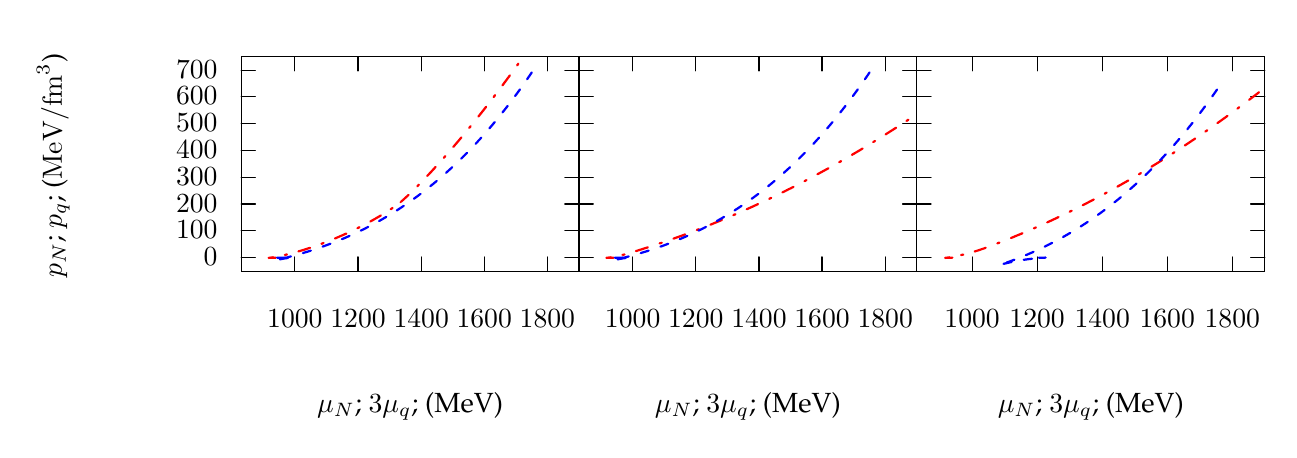
\begin{tikzpicture}[gnuplot]
%% generated with GNUPLOT 5.0p4 (Lua 5.2; terminal rev. 99, script rev. 100)
%% Mon Nov 28 17:06:57 2016
\path (0.000,0.000) rectangle (13.000,5.000);
\gpcolor{color=gp lt color border}
\gpsetlinetype{gp lt border}
\gpsetdashtype{gp dt solid}
\gpsetlinewidth{1.00}
\draw[gp path] (0.000,2.079)--(0.180,2.079);
\draw[gp path] (4.289,2.079)--(4.109,2.079);
\node[gp node right] at (-0.184,2.079) {$0$};
\draw[gp path] (0.000,2.419)--(0.180,2.419);
\draw[gp path] (4.289,2.419)--(4.109,2.419);
\node[gp node right] at (-0.184,2.419) {$100$};
\draw[gp path] (0.000,2.760)--(0.180,2.760);
\draw[gp path] (4.289,2.760)--(4.109,2.760);
\node[gp node right] at (-0.184,2.760) {$200$};
\draw[gp path] (0.000,3.100)--(0.180,3.100);
\draw[gp path] (4.289,3.100)--(4.109,3.100);
\node[gp node right] at (-0.184,3.100) {$300$};
\draw[gp path] (0.000,3.440)--(0.180,3.440);
\draw[gp path] (4.289,3.440)--(4.109,3.440);
\node[gp node right] at (-0.184,3.440) {$400$};
\draw[gp path] (0.000,3.780)--(0.180,3.780);
\draw[gp path] (4.289,3.780)--(4.109,3.780);
\node[gp node right] at (-0.184,3.780) {$500$};
\draw[gp path] (0.000,4.121)--(0.180,4.121);
\draw[gp path] (4.289,4.121)--(4.109,4.121);
\node[gp node right] at (-0.184,4.121) {$600$};
\draw[gp path] (0.000,4.461)--(0.180,4.461);
\draw[gp path] (4.289,4.461)--(4.109,4.461);
\node[gp node right] at (-0.184,4.461) {$700$};
\draw[gp path] (0.681,1.909)--(0.681,2.089);
\draw[gp path] (0.681,4.631)--(0.681,4.451);
\node[gp node center] at (0.681,1.293) {$1000$};
\draw[gp path] (1.483,1.909)--(1.483,2.089);
\draw[gp path] (1.483,4.631)--(1.483,4.451);
\node[gp node center] at (1.483,1.293) {$1200$};
\draw[gp path] (2.285,1.909)--(2.285,2.089);
\draw[gp path] (2.285,4.631)--(2.285,4.451);
\node[gp node center] at (2.285,1.293) {$1400$};
\draw[gp path] (3.086,1.909)--(3.086,2.089);
\draw[gp path] (3.086,4.631)--(3.086,4.451);
\node[gp node center] at (3.086,1.293) {$1600$};
\draw[gp path] (3.888,1.909)--(3.888,2.089);
\draw[gp path] (3.888,4.631)--(3.888,4.451);
\node[gp node center] at (3.888,1.293) {$1800$};
\draw[gp path] (0.000,4.631)--(0.000,1.909)--(4.289,1.909)--(4.289,4.631)--cycle;
\node[gp node center,rotate=-270] at (-2.362,3.270) {$p_N$; $p_q$; ($\rm{MeV}/\rm{fm}^3$)};
\node[gp node center] at (2.144,0.215) {$\mu_N$; $3\mu_q$; (MeV)};
\gpcolor{rgb color={1.000,0.000,0.000}}
\gpsetdashtype{gp dt 6}
\gpsetlinewidth{2.00}
\draw[gp path] (0.439,2.079)--(0.438,2.079)--(0.437,2.079)--(0.436,2.079)--(0.435,2.079)%
  --(0.434,2.079)--(0.433,2.079)--(0.432,2.079)--(0.431,2.079)--(0.430,2.079)--(0.429,2.079)%
  --(0.428,2.079)--(0.427,2.079)--(0.426,2.079)--(0.425,2.079)--(0.424,2.079)--(0.423,2.079)%
  --(0.422,2.079)--(0.421,2.079)--(0.420,2.079)--(0.419,2.079)--(0.418,2.079)--(0.417,2.079)%
  --(0.416,2.079)--(0.415,2.079)--(0.414,2.079)--(0.413,2.079)--(0.412,2.079)--(0.411,2.079)%
  --(0.410,2.079)--(0.409,2.079)--(0.408,2.079)--(0.407,2.079)--(0.406,2.079)--(0.405,2.079)%
  --(0.404,2.079)--(0.403,2.079)--(0.402,2.079)--(0.401,2.079)--(0.400,2.079)--(0.399,2.079)%
  --(0.398,2.079)--(0.397,2.079)--(0.396,2.078)--(0.395,2.078)--(0.394,2.078)--(0.393,2.078)%
  --(0.392,2.078)--(0.391,2.078)--(0.390,2.078)--(0.389,2.078)--(0.388,2.078)--(0.387,2.078)%
  --(0.386,2.078)--(0.385,2.078)--(0.384,2.078)--(0.383,2.078)--(0.382,2.078)--(0.381,2.078)%
  --(0.380,2.078)--(0.379,2.078)--(0.378,2.078)--(0.377,2.078)--(0.376,2.078)--(0.375,2.078)%
  --(0.374,2.078)--(0.373,2.078)--(0.372,2.078)--(0.371,2.078)--(0.370,2.078)--(0.370,2.077)%
  --(0.369,2.077)--(0.368,2.077)--(0.367,2.077)--(0.366,2.077)--(0.365,2.077)--(0.364,2.077)%
  --(0.363,2.077)--(0.362,2.077)--(0.361,2.077)--(0.360,2.077)--(0.359,2.077)--(0.358,2.077)%
  --(0.357,2.077)--(0.356,2.077)--(0.355,2.077)--(0.354,2.077)--(0.353,2.077)--(0.352,2.077)%
  --(0.352,2.076)--(0.351,2.076)--(0.350,2.076)--(0.349,2.076)--(0.348,2.076)--(0.347,2.076)%
  --(0.348,2.076)--(0.349,2.076)--(0.350,2.076)--(0.351,2.076)--(0.351,2.077)--(0.352,2.077)%
  --(0.353,2.077)--(0.354,2.077)--(0.355,2.077)--(0.356,2.077)--(0.357,2.077)--(0.358,2.077)%
  --(0.359,2.077)--(0.360,2.077)--(0.360,2.078)--(0.361,2.078)--(0.362,2.078)--(0.363,2.078)%
  --(0.364,2.078)--(0.365,2.078)--(0.366,2.078)--(0.367,2.078)--(0.368,2.079)--(0.369,2.079)%
  --(0.370,2.079)--(0.371,2.079)--(0.372,2.079)--(0.373,2.079)--(0.374,2.079)--(0.375,2.080)%
  --(0.376,2.080)--(0.377,2.080)--(0.378,2.080)--(0.379,2.080)--(0.380,2.080)--(0.381,2.080)%
  --(0.382,2.080)--(0.382,2.081)--(0.383,2.081)--(0.384,2.081)--(0.385,2.081)--(0.386,2.081)%
  --(0.387,2.081)--(0.388,2.081)--(0.389,2.082)--(0.390,2.082)--(0.391,2.082)--(0.392,2.082)%
  --(0.393,2.082)--(0.394,2.082)--(0.395,2.082)--(0.396,2.083)--(0.397,2.083)--(0.398,2.083)%
  --(0.399,2.083)--(0.400,2.083)--(0.401,2.083)--(0.402,2.084)--(0.403,2.084)--(0.404,2.084)%
  --(0.405,2.084)--(0.406,2.084)--(0.407,2.084)--(0.408,2.085)--(0.409,2.085)--(0.410,2.085)%
  --(0.411,2.085)--(0.412,2.085)--(0.413,2.085)--(0.414,2.086)--(0.415,2.086)--(0.416,2.086)%
  --(0.417,2.086)--(0.418,2.086)--(0.419,2.086)--(0.420,2.087)--(0.421,2.087)--(0.422,2.087)%
  --(0.423,2.087)--(0.424,2.087)--(0.425,2.087)--(0.426,2.088)--(0.427,2.088)--(0.428,2.088)%
  --(0.429,2.088)--(0.430,2.088)--(0.431,2.088)--(0.432,2.089)--(0.433,2.089)--(0.434,2.089)%
  --(0.435,2.089)--(0.437,2.089)--(0.438,2.090)--(0.439,2.090)--(0.440,2.090)--(0.441,2.090)%
  --(0.442,2.090)--(0.443,2.091)--(0.444,2.091)--(0.445,2.091)--(0.446,2.091)--(0.447,2.091)%
  --(0.449,2.092)--(0.450,2.092)--(0.451,2.092)--(0.452,2.092)--(0.453,2.092)--(0.454,2.093)%
  --(0.455,2.093)--(0.457,2.093)--(0.458,2.093)--(0.459,2.094)--(0.460,2.094)--(0.461,2.094)%
  --(0.463,2.094)--(0.464,2.094)--(0.465,2.095)--(0.466,2.095)--(0.467,2.095)--(0.469,2.095)%
  --(0.470,2.096)--(0.471,2.096)--(0.472,2.096)--(0.473,2.096)--(0.475,2.097)--(0.476,2.097)%
  --(0.477,2.097)--(0.478,2.097)--(0.480,2.098)--(0.481,2.098)--(0.482,2.098)--(0.484,2.098)%
  --(0.485,2.099)--(0.486,2.099)--(0.487,2.099)--(0.489,2.099)--(0.490,2.100)--(0.491,2.100)%
  --(0.493,2.100)--(0.494,2.101)--(0.495,2.101)--(0.497,2.101)--(0.498,2.101)--(0.499,2.102)%
  --(0.501,2.102)--(0.502,2.102)--(0.503,2.102)--(0.505,2.103)--(0.506,2.103)--(0.507,2.103)%
  --(0.509,2.104)--(0.510,2.104)--(0.511,2.104)--(0.513,2.105)--(0.514,2.105)--(0.516,2.105)%
  --(0.517,2.105)--(0.518,2.106)--(0.520,2.106)--(0.521,2.106)--(0.523,2.107)--(0.524,2.107)%
  --(0.525,2.107)--(0.527,2.108)--(0.528,2.108)--(0.530,2.108)--(0.531,2.109)--(0.533,2.109)%
  --(0.534,2.109)--(0.535,2.109)--(0.537,2.110)--(0.538,2.110)--(0.540,2.110)--(0.541,2.111)%
  --(0.543,2.111)--(0.544,2.111)--(0.546,2.112)--(0.547,2.112)--(0.549,2.112)--(0.550,2.113)%
  --(0.552,2.113)--(0.553,2.114)--(0.555,2.114)--(0.556,2.114)--(0.558,2.115)--(0.559,2.115)%
  --(0.561,2.115)--(0.562,2.116)--(0.564,2.116)--(0.565,2.116)--(0.567,2.117)--(0.568,2.117)%
  --(0.570,2.117)--(0.572,2.118)--(0.573,2.118)--(0.575,2.119)--(0.576,2.119)--(0.578,2.119)%
  --(0.579,2.120)--(0.581,2.120)--(0.583,2.120)--(0.584,2.121)--(0.586,2.121)--(0.587,2.122)%
  --(0.589,2.122)--(0.590,2.122)--(0.592,2.123)--(0.594,2.123)--(0.595,2.124)--(0.597,2.124)%
  --(0.599,2.124)--(0.600,2.125)--(0.602,2.125)--(0.603,2.126)--(0.605,2.126)--(0.607,2.126)%
  --(0.608,2.127)--(0.610,2.127)--(0.612,2.128)--(0.613,2.128)--(0.615,2.128)--(0.617,2.129)%
  --(0.618,2.129)--(0.620,2.130)--(0.622,2.130)--(0.623,2.131)--(0.625,2.131)--(0.627,2.131)%
  --(0.628,2.132)--(0.630,2.132)--(0.632,2.133)--(0.633,2.133)--(0.635,2.134)--(0.637,2.134)%
  --(0.638,2.134)--(0.640,2.135)--(0.642,2.135)--(0.644,2.136)--(0.645,2.136)--(0.647,2.137)%
  --(0.649,2.137)--(0.650,2.138)--(0.652,2.138)--(0.654,2.139)--(0.656,2.139)--(0.657,2.139)%
  --(0.659,2.140)--(0.661,2.140)--(0.663,2.141)--(0.664,2.141)--(0.666,2.142)--(0.668,2.142)%
  --(0.670,2.143)--(0.671,2.143)--(0.673,2.144)--(0.675,2.144)--(0.677,2.145)--(0.678,2.145)%
  --(0.680,2.146)--(0.682,2.146)--(0.684,2.147)--(0.686,2.147)--(0.687,2.148)--(0.689,2.148)%
  --(0.691,2.149)--(0.693,2.149)--(0.695,2.150)--(0.696,2.150)--(0.698,2.151)--(0.700,2.151)%
  --(0.702,2.152)--(0.704,2.152)--(0.705,2.153)--(0.707,2.153)--(0.709,2.154)--(0.711,2.154)%
  --(0.713,2.155)--(0.715,2.155)--(0.716,2.156)--(0.718,2.156)--(0.720,2.157)--(0.722,2.157)%
  --(0.724,2.158)--(0.726,2.158)--(0.728,2.159)--(0.729,2.160)--(0.731,2.160)--(0.733,2.161)%
  --(0.735,2.161)--(0.737,2.162)--(0.739,2.162)--(0.741,2.163)--(0.742,2.163)--(0.744,2.164)%
  --(0.746,2.164)--(0.748,2.165)--(0.750,2.166)--(0.752,2.166)--(0.754,2.167)--(0.756,2.167)%
  --(0.758,2.168)--(0.759,2.168)--(0.761,2.169)--(0.763,2.169)--(0.765,2.170)--(0.767,2.171)%
  --(0.769,2.171)--(0.771,2.172)--(0.773,2.172)--(0.775,2.173)--(0.777,2.174)--(0.779,2.174)%
  --(0.780,2.175)--(0.782,2.175)--(0.784,2.176)--(0.786,2.176)--(0.788,2.177)--(0.790,2.178)%
  --(0.792,2.178)--(0.794,2.179)--(0.796,2.179)--(0.798,2.180)--(0.800,2.181)--(0.802,2.181)%
  --(0.804,2.182)--(0.806,2.182)--(0.808,2.183)--(0.810,2.184)--(0.812,2.184)--(0.813,2.185)%
  --(0.815,2.186)--(0.817,2.186)--(0.819,2.187)--(0.821,2.187)--(0.823,2.188)--(0.825,2.189)%
  --(0.827,2.189)--(0.829,2.190)--(0.831,2.191)--(0.833,2.191)--(0.835,2.192)--(0.837,2.192)%
  --(0.839,2.193)--(0.841,2.194)--(0.843,2.194)--(0.845,2.195)--(0.847,2.196)--(0.849,2.196)%
  --(0.851,2.197)--(0.853,2.198)--(0.855,2.198)--(0.857,2.199)--(0.859,2.200)--(0.861,2.200)%
  --(0.863,2.201)--(0.865,2.201)--(0.867,2.202)--(0.869,2.203)--(0.871,2.203)--(0.873,2.204)%
  --(0.875,2.205)--(0.877,2.205)--(0.879,2.206)--(0.881,2.207)--(0.883,2.208)--(0.885,2.208)%
  --(0.887,2.209)--(0.889,2.210)--(0.891,2.210)--(0.893,2.211)--(0.895,2.212)--(0.897,2.212)%
  --(0.899,2.213)--(0.901,2.214)--(0.903,2.214)--(0.906,2.215)--(0.908,2.216)--(0.910,2.216)%
  --(0.912,2.217)--(0.914,2.218)--(0.916,2.219)--(0.918,2.219)--(0.920,2.220)--(0.922,2.221)%
  --(0.924,2.221)--(0.926,2.222)--(0.928,2.223)--(0.930,2.223)--(0.932,2.224)--(0.934,2.225)%
  --(0.936,2.226)--(0.938,2.226)--(0.940,2.227)--(0.942,2.228)--(0.944,2.229)--(0.947,2.229)%
  --(0.949,2.230)--(0.951,2.231)--(0.953,2.231)--(0.955,2.232)--(0.957,2.233)--(0.959,2.234)%
  --(0.961,2.234)--(0.963,2.235)--(0.965,2.236)--(0.967,2.237)--(0.969,2.237)--(0.971,2.238)%
  --(0.973,2.239)--(0.976,2.240)--(0.978,2.240)--(0.980,2.241)--(0.982,2.242)--(0.984,2.243)%
  --(0.986,2.243)--(0.988,2.244)--(0.990,2.245)--(0.992,2.246)--(0.994,2.246)--(0.996,2.247)%
  --(0.998,2.248)--(1.001,2.249)--(1.003,2.249)--(1.005,2.250)--(1.007,2.251)--(1.009,2.252)%
  --(1.011,2.252)--(1.013,2.253)--(1.015,2.254)--(1.017,2.255)--(1.019,2.256)--(1.021,2.256)%
  --(1.024,2.257)--(1.026,2.258)--(1.028,2.259)--(1.030,2.259)--(1.032,2.260)--(1.034,2.261)%
  --(1.036,2.262)--(1.038,2.263)--(1.040,2.263)--(1.042,2.264)--(1.044,2.265)--(1.047,2.266)%
  --(1.049,2.267)--(1.051,2.267)--(1.053,2.268)--(1.055,2.269)--(1.057,2.270)--(1.059,2.271)%
  --(1.061,2.271)--(1.063,2.272)--(1.065,2.273)--(1.068,2.274)--(1.070,2.275)--(1.072,2.275)%
  --(1.074,2.276)--(1.076,2.277)--(1.078,2.278)--(1.080,2.279)--(1.082,2.279)--(1.084,2.280)%
  --(1.087,2.281)--(1.089,2.282)--(1.091,2.283)--(1.093,2.284)--(1.095,2.284)--(1.097,2.285)%
  --(1.099,2.286)--(1.101,2.287)--(1.103,2.288)--(1.105,2.289)--(1.108,2.289)--(1.110,2.290)%
  --(1.112,2.291)--(1.114,2.292)--(1.116,2.293)--(1.118,2.294)--(1.120,2.294)--(1.122,2.295)%
  --(1.124,2.296)--(1.127,2.297)--(1.129,2.298)--(1.131,2.299)--(1.133,2.299)--(1.135,2.300)%
  --(1.137,2.301)--(1.139,2.302)--(1.141,2.303)--(1.143,2.304)--(1.146,2.305)--(1.148,2.305)%
  --(1.150,2.306)--(1.152,2.307)--(1.154,2.308)--(1.156,2.309)--(1.158,2.310)--(1.160,2.311)%
  --(1.162,2.311)--(1.164,2.312)--(1.167,2.313)--(1.169,2.314)--(1.171,2.315)--(1.173,2.316)%
  --(1.175,2.317)--(1.177,2.317)--(1.179,2.318)--(1.181,2.319)--(1.183,2.320)--(1.185,2.321)%
  --(1.188,2.322)--(1.190,2.323)--(1.192,2.324)--(1.194,2.324)--(1.196,2.325)--(1.198,2.326)%
  --(1.200,2.327)--(1.202,2.328)--(1.204,2.329)--(1.206,2.330)--(1.209,2.331)--(1.211,2.332)%
  --(1.213,2.332)--(1.215,2.333)--(1.217,2.334)--(1.219,2.335)--(1.221,2.336)--(1.223,2.337)%
  --(1.225,2.338)--(1.227,2.339)--(1.229,2.340)--(1.232,2.340)--(1.234,2.341)--(1.236,2.342)%
  --(1.238,2.343)--(1.240,2.344)--(1.242,2.345)--(1.244,2.346)--(1.246,2.347)--(1.248,2.348)%
  --(1.250,2.349)--(1.252,2.349)--(1.254,2.350)--(1.257,2.351)--(1.259,2.352)--(1.261,2.353)%
  --(1.263,2.354)--(1.265,2.355)--(1.267,2.356)--(1.269,2.357)--(1.271,2.358)--(1.273,2.359)%
  --(1.275,2.359)--(1.277,2.360)--(1.279,2.361)--(1.281,2.362)--(1.284,2.363)--(1.286,2.364)%
  --(1.288,2.365)--(1.290,2.366)--(1.292,2.367)--(1.294,2.368)--(1.296,2.369)--(1.298,2.369)%
  --(1.300,2.370)--(1.302,2.371)--(1.304,2.372)--(1.306,2.373)--(1.308,2.374)--(1.310,2.375)%
  --(1.312,2.376)--(1.314,2.377)--(1.316,2.378)--(1.318,2.379)--(1.321,2.380)--(1.323,2.381)%
  --(1.325,2.382)--(1.327,2.382)--(1.329,2.383)--(1.331,2.384)--(1.333,2.385)--(1.335,2.386)%
  --(1.337,2.387)--(1.339,2.388)--(1.341,2.389)--(1.343,2.390)--(1.345,2.391)--(1.347,2.392)%
  --(1.349,2.393)--(1.351,2.394)--(1.353,2.395)--(1.355,2.395)--(1.357,2.396)--(1.359,2.397)%
  --(1.361,2.398)--(1.363,2.399)--(1.365,2.400)--(1.367,2.401)--(1.369,2.402)--(1.371,2.403)%
  --(1.373,2.404)--(1.375,2.405)--(1.377,2.406)--(1.379,2.407)--(1.381,2.408)--(1.383,2.409)%
  --(1.385,2.410)--(1.387,2.411)--(1.389,2.411)--(1.391,2.412)--(1.393,2.413)--(1.395,2.414)%
  --(1.397,2.415)--(1.399,2.416)--(1.401,2.417)--(1.403,2.418)--(1.405,2.419)--(1.407,2.420)%
  --(1.409,2.421)--(1.411,2.422)--(1.413,2.423)--(1.415,2.424)--(1.417,2.425)--(1.419,2.426)%
  --(1.421,2.427)--(1.423,2.428)--(1.425,2.428)--(1.427,2.429)--(1.429,2.430)--(1.431,2.431)%
  --(1.433,2.432)--(1.435,2.433)--(1.437,2.434)--(1.439,2.435)--(1.441,2.436)--(1.443,2.437)%
  --(1.444,2.438)--(1.446,2.439)--(1.448,2.440)--(1.450,2.441)--(1.452,2.442)--(1.454,2.443)%
  --(1.456,2.444)--(1.458,2.445)--(1.460,2.446)--(1.462,2.446)--(1.464,2.447)--(1.466,2.448)%
  --(1.468,2.449)--(1.470,2.450)--(1.471,2.451)--(1.473,2.452)--(1.475,2.453)--(1.477,2.454)%
  --(1.479,2.455)--(1.481,2.456)--(1.483,2.457)--(1.485,2.458)--(1.487,2.459)--(1.489,2.460)%
  --(1.491,2.461)--(1.492,2.462)--(1.494,2.463)--(1.496,2.464)--(1.498,2.465)--(1.500,2.465)%
  --(1.502,2.466)--(1.504,2.467)--(1.506,2.468)--(1.507,2.469)--(1.509,2.470)--(1.511,2.471)%
  --(1.513,2.472)--(1.515,2.473)--(1.517,2.474)--(1.519,2.475)--(1.521,2.476)--(1.522,2.477)%
  --(1.524,2.478)--(1.526,2.479)--(1.528,2.480)--(1.530,2.481)--(1.532,2.482)--(1.533,2.483)%
  --(1.535,2.483)--(1.537,2.484)--(1.539,2.485)--(1.541,2.486)--(1.543,2.487)--(1.544,2.488)%
  --(1.546,2.489)--(1.548,2.490)--(1.550,2.491)--(1.552,2.492)--(1.554,2.493)--(1.555,2.494)%
  --(1.557,2.495)--(1.559,2.496)--(1.561,2.497)--(1.563,2.498)--(1.564,2.499)--(1.566,2.500)%
  --(1.568,2.500)--(1.570,2.501)--(1.571,2.502)--(1.573,2.503)--(1.575,2.504)--(1.577,2.505)%
  --(1.579,2.506)--(1.580,2.507)--(1.582,2.508)--(1.584,2.509)--(1.586,2.510)--(1.587,2.511)%
  --(1.589,2.512)--(1.591,2.513)--(1.593,2.514)--(1.594,2.514)--(1.596,2.515)--(1.598,2.516)%
  --(1.600,2.517)--(1.601,2.518)--(1.603,2.519)--(1.605,2.520)--(1.607,2.521)--(1.608,2.522)%
  --(1.610,2.523)--(1.612,2.524)--(1.613,2.525)--(1.615,2.526)--(1.617,2.527)--(1.619,2.527)%
  --(1.620,2.528)--(1.622,2.529)--(1.624,2.530)--(1.625,2.531)--(1.627,2.532)--(1.629,2.533)%
  --(1.630,2.534)--(1.632,2.535)--(1.634,2.536)--(1.635,2.537)--(1.637,2.538)--(1.639,2.538)%
  --(1.640,2.539)--(1.642,2.540)--(1.644,2.541)--(1.645,2.542)--(1.647,2.543)--(1.649,2.544)%
  --(1.650,2.545)--(1.652,2.546)--(1.654,2.547)--(1.655,2.548)--(1.657,2.548)--(1.658,2.549)%
  --(1.660,2.550)--(1.662,2.551)--(1.663,2.552)--(1.665,2.553)--(1.667,2.554)--(1.668,2.555)%
  --(1.670,2.556)--(1.671,2.557)--(1.673,2.557)--(1.675,2.558)--(1.676,2.559)--(1.678,2.560)%
  --(1.679,2.561)--(1.681,2.562)--(1.683,2.563)--(1.684,2.564)--(1.686,2.565)--(1.687,2.565)%
  --(1.689,2.566)--(1.690,2.567)--(1.692,2.568)--(1.693,2.569)--(1.695,2.570)--(1.697,2.571)%
  --(1.698,2.572)--(1.700,2.573)--(1.701,2.573)--(1.703,2.574)--(1.704,2.575)--(1.706,2.576)%
  --(1.707,2.577)--(1.709,2.578)--(1.710,2.579)--(1.712,2.580)--(1.713,2.580)--(1.715,2.581)%
  --(1.716,2.582)--(1.718,2.583)--(1.719,2.584)--(1.721,2.585)--(1.722,2.586)--(1.724,2.586)%
  --(1.725,2.587)--(1.727,2.588)--(1.728,2.589)--(1.730,2.590)--(1.731,2.591)--(1.733,2.592)%
  --(1.734,2.592)--(1.736,2.593)--(1.737,2.594)--(1.738,2.595)--(1.740,2.596)--(1.741,2.597)%
  --(1.743,2.597)--(1.744,2.598)--(1.746,2.599)--(1.747,2.600)--(1.749,2.601)--(1.750,2.602)%
  --(1.751,2.602)--(1.753,2.603)--(1.754,2.604)--(1.756,2.605)--(1.757,2.606)--(1.758,2.607)%
  --(1.760,2.607)--(1.761,2.608)--(1.763,2.609)--(1.764,2.610)--(1.765,2.611)--(1.767,2.612)%
  --(1.768,2.612)--(1.769,2.613)--(1.771,2.614)--(1.772,2.615)--(1.773,2.616)--(1.775,2.616)%
  --(1.776,2.617)--(1.777,2.618)--(1.779,2.619)--(1.780,2.620)--(1.781,2.620)--(1.783,2.621)%
  --(1.784,2.622)--(1.785,2.623)--(1.787,2.624)--(1.788,2.624)--(1.789,2.625)--(1.791,2.626)%
  --(1.792,2.627)--(1.793,2.628)--(1.795,2.628)--(1.796,2.629)--(1.797,2.630)--(1.798,2.631)%
  --(1.800,2.631)--(1.801,2.632)--(1.802,2.633)--(1.803,2.634)--(1.805,2.635)--(1.806,2.635)%
  --(1.807,2.636)--(1.808,2.637)--(1.810,2.638)--(1.811,2.638)--(1.812,2.639)--(1.813,2.640)%
  --(1.815,2.641)--(1.816,2.641)--(1.817,2.642)--(1.818,2.643)--(1.819,2.644)--(1.821,2.644)%
  --(1.822,2.645)--(1.823,2.646)--(1.824,2.647)--(1.825,2.647)--(1.827,2.648)--(1.828,2.649)%
  --(1.829,2.650)--(1.830,2.650)--(1.831,2.651)--(1.833,2.652)--(1.834,2.653)--(1.835,2.653)%
  --(1.836,2.654)--(1.837,2.655)--(1.838,2.655)--(1.839,2.656)--(1.841,2.657)--(1.842,2.658)%
  --(1.843,2.658)--(1.844,2.659)--(1.845,2.660)--(1.846,2.660)--(1.847,2.661)--(1.848,2.662)%
  --(1.849,2.662)--(1.851,2.663)--(1.852,2.664)--(1.853,2.665)--(1.854,2.665)--(1.855,2.666)%
  --(1.856,2.667)--(1.857,2.667)--(1.858,2.668)--(1.859,2.669)--(1.860,2.669)--(1.861,2.670)%
  --(1.862,2.671)--(1.863,2.671)--(1.864,2.672)--(1.865,2.673)--(1.867,2.673)--(1.868,2.674)%
  --(1.869,2.675)--(1.870,2.675)--(1.871,2.676)--(1.872,2.677)--(1.873,2.677)--(1.874,2.678)%
  --(1.875,2.679)--(1.876,2.679)--(1.877,2.680)--(1.878,2.681)--(1.879,2.681)--(1.880,2.682)%
  --(1.881,2.682)--(1.882,2.683)--(1.882,2.684)--(1.883,2.684)--(1.884,2.685)--(1.885,2.686)%
  --(1.886,2.686)--(1.887,2.687)--(1.888,2.687)--(1.889,2.688)--(1.890,2.689)--(1.891,2.689)%
  --(1.892,2.690)--(1.893,2.690)--(1.894,2.691)--(1.895,2.692)--(1.896,2.692)--(1.896,2.693)%
  --(1.897,2.693)--(1.898,2.694)--(1.899,2.695)--(1.900,2.695)--(1.901,2.696)--(1.902,2.696)%
  --(1.903,2.697)--(1.904,2.698)--(1.905,2.699)--(1.906,2.699)--(1.907,2.700)--(1.908,2.700)%
  --(1.909,2.701)--(1.910,2.702)--(1.911,2.703)--(1.912,2.703)--(1.913,2.704)--(1.914,2.704)%
  --(1.915,2.705)--(1.916,2.706)--(1.917,2.707)--(1.918,2.707)--(1.919,2.708)--(1.920,2.709)%
  --(1.921,2.709)--(1.922,2.710)--(1.923,2.711)--(1.924,2.711)--(1.925,2.712)--(1.926,2.713)%
  --(1.927,2.713)--(1.928,2.714)--(1.929,2.715)--(1.930,2.715)--(1.931,2.716)--(1.932,2.717)%
  --(1.933,2.717)--(1.934,2.718)--(1.935,2.719)--(1.936,2.719)--(1.936,2.720)--(1.937,2.720)%
  --(1.938,2.721)--(1.939,2.722)--(1.940,2.722)--(1.940,2.723)--(1.941,2.723)--(1.942,2.724)%
  --(1.943,2.724)--(1.944,2.725)--(1.945,2.726)--(1.946,2.726)--(1.946,2.727)--(1.947,2.727)%
  --(1.948,2.728)--(1.949,2.728)--(1.949,2.729)--(1.950,2.729)--(1.951,2.730)--(1.952,2.731)%
  --(1.953,2.731)--(1.954,2.732)--(1.955,2.733)--(1.956,2.733)--(1.957,2.734)--(1.958,2.735)%
  --(1.959,2.735)--(1.959,2.736)--(1.960,2.736)--(1.960,2.737)--(1.961,2.737)--(1.962,2.737)%
  --(1.962,2.738)--(1.963,2.738)--(1.964,2.739)--(1.965,2.740)--(1.966,2.740)--(1.966,2.741)%
  --(1.967,2.741)--(1.968,2.742)--(1.969,2.742)--(1.969,2.743)--(1.970,2.743)--(1.971,2.744)%
  --(1.971,2.745)--(1.972,2.745)--(1.973,2.746)--(1.974,2.746)--(1.975,2.747)--(1.976,2.747)%
  --(1.976,2.748)--(1.977,2.748)--(1.977,2.749)--(1.978,2.749)--(1.978,2.750)--(1.979,2.750)%
  --(1.980,2.750)--(1.980,2.751)--(1.981,2.751)--(1.981,2.752)--(1.982,2.752)--(1.983,2.753)%
  --(1.984,2.753)--(1.984,2.754)--(1.985,2.754)--(1.985,2.755)--(1.986,2.755)--(1.987,2.756)%
  --(1.988,2.756)--(1.988,2.757)--(1.989,2.757)--(1.989,2.758)--(1.990,2.758)--(1.991,2.759)%
  --(1.992,2.759)--(1.992,2.760)--(1.993,2.760)--(1.993,2.761)--(1.994,2.761)--(1.995,2.762)%
  --(1.996,2.762)--(1.996,2.763)--(1.997,2.763)--(1.997,2.764)--(1.998,2.764)--(1.999,2.765)%
  --(2.000,2.765)--(2.000,2.766)--(2.001,2.766)--(2.001,2.767)--(2.002,2.767)--(2.002,2.768)%
  --(2.003,2.768)--(2.004,2.769)--(2.005,2.769)--(2.005,2.770)--(2.006,2.770)--(2.006,2.771)%
  --(2.007,2.771)--(2.007,2.772)--(2.008,2.772)--(2.009,2.772)--(2.009,2.773)--(2.010,2.773)%
  --(2.010,2.774)--(2.011,2.774)--(2.011,2.775)--(2.012,2.775)--(2.012,2.776)--(2.013,2.776)%
  --(2.014,2.776)--(2.014,2.777)--(2.015,2.777)--(2.015,2.778)--(2.016,2.778)--(2.016,2.779)%
  --(2.017,2.779)--(2.017,2.780)--(2.018,2.780)--(2.019,2.781)--(2.020,2.781)--(2.020,2.782)%
  --(2.021,2.782)--(2.021,2.783)--(2.022,2.783)--(2.022,2.784)--(2.023,2.784)--(2.023,2.785)%
  --(2.024,2.785)--(2.024,2.786)--(2.025,2.786)--(2.026,2.786)--(2.026,2.787)--(2.027,2.787)%
  --(2.027,2.788)--(2.028,2.788)--(2.028,2.789)--(2.029,2.789)--(2.029,2.790)--(2.030,2.790)%
  --(2.030,2.791)--(2.031,2.791)--(2.032,2.792)--(2.033,2.793)--(2.034,2.793)--(2.034,2.794)%
  --(2.035,2.794)--(2.035,2.795)--(2.036,2.795)--(2.036,2.796)--(2.037,2.796)--(2.038,2.797)%
  --(2.039,2.798)--(2.040,2.799)--(2.041,2.800)--(2.042,2.801)--(2.043,2.801)--(2.043,2.802)%
  --(2.044,2.802)--(2.044,2.803)--(2.045,2.803)--(2.045,2.804)--(2.046,2.804)--(2.047,2.805)%
  --(2.048,2.806)--(2.049,2.807)--(2.050,2.807)--(2.050,2.808)--(2.051,2.808)--(2.051,2.809)%
  --(2.052,2.809)--(2.052,2.810)--(2.053,2.810)--(2.053,2.811)--(2.054,2.811)--(2.054,2.812)%
  --(2.055,2.812)--(2.056,2.813)--(2.057,2.814)--(2.058,2.815)--(2.059,2.816)--(2.060,2.817)%
  --(2.061,2.818)--(2.062,2.818)--(2.063,2.819)--(2.064,2.820)--(2.065,2.821)--(2.066,2.822)%
  --(2.066,2.823)--(2.067,2.823)--(2.068,2.824)--(2.069,2.825)--(2.070,2.826)--(2.071,2.826)%
  --(2.071,2.827)--(2.072,2.827)--(2.072,2.828)--(2.073,2.828)--(2.074,2.829)--(2.074,2.830)%
  --(2.075,2.830)--(2.075,2.831)--(2.076,2.831)--(2.077,2.832)--(2.077,2.833)--(2.078,2.833)%
  --(2.079,2.834)--(2.080,2.835)--(2.081,2.836)--(2.082,2.837)--(2.083,2.837)--(2.083,2.838)%
  --(2.084,2.839)--(2.085,2.839)--(2.085,2.840)--(2.086,2.841)--(2.087,2.841)--(2.088,2.842)%
  --(2.088,2.843)--(2.089,2.843)--(2.090,2.844)--(2.090,2.845)--(2.091,2.845)--(2.092,2.846)%
  --(2.093,2.847)--(2.094,2.848)--(2.095,2.849)--(2.096,2.849)--(2.096,2.850)--(2.097,2.851)%
  --(2.098,2.852)--(2.099,2.852)--(2.099,2.853)--(2.100,2.854)--(2.101,2.854)--(2.102,2.855)%
  --(2.103,2.856)--(2.103,2.857)--(2.104,2.857)--(2.105,2.858)--(2.106,2.859)--(2.107,2.860)%
  --(2.108,2.861)--(2.109,2.862)--(2.110,2.863)--(2.111,2.864)--(2.112,2.864)--(2.112,2.865)%
  --(2.113,2.866)--(2.114,2.867)--(2.115,2.868)--(2.116,2.868)--(2.117,2.869)--(2.118,2.870)%
  --(2.118,2.871)--(2.119,2.872)--(2.120,2.873)--(2.121,2.873)--(2.122,2.874)--(2.123,2.875)%
  --(2.124,2.876)--(2.125,2.877)--(2.126,2.878)--(2.127,2.879)--(2.128,2.880)--(2.129,2.881)%
  --(2.130,2.882)--(2.131,2.883)--(2.132,2.884)--(2.133,2.885)--(2.134,2.886)--(2.135,2.887)%
  --(2.136,2.888)--(2.137,2.888)--(2.138,2.889)--(2.139,2.890)--(2.140,2.891)--(2.141,2.892)%
  --(2.142,2.893)--(2.143,2.894)--(2.144,2.895)--(2.145,2.896)--(2.146,2.897)--(2.147,2.898)%
  --(2.148,2.899)--(2.149,2.900)--(2.150,2.901)--(2.151,2.902)--(2.152,2.903)--(2.153,2.904)%
  --(2.154,2.905)--(2.155,2.906)--(2.156,2.907)--(2.157,2.908)--(2.158,2.909)--(2.159,2.910)%
  --(2.160,2.911)--(2.161,2.912)--(2.162,2.913)--(2.163,2.914)--(2.164,2.915)--(2.165,2.916)%
  --(2.167,2.917)--(2.168,2.918)--(2.169,2.919)--(2.170,2.920)--(2.171,2.921)--(2.172,2.923)%
  --(2.173,2.924)--(2.174,2.925)--(2.175,2.926)--(2.176,2.927)--(2.178,2.928)--(2.179,2.929)%
  --(2.180,2.930)--(2.181,2.931)--(2.182,2.932)--(2.183,2.934)--(2.184,2.935)--(2.185,2.936)%
  --(2.187,2.937)--(2.188,2.938)--(2.189,2.939)--(2.190,2.940)--(2.191,2.942)--(2.192,2.943)%
  --(2.194,2.944)--(2.195,2.945)--(2.196,2.946)--(2.197,2.947)--(2.198,2.949)--(2.200,2.950)%
  --(2.201,2.951)--(2.202,2.952)--(2.203,2.953)--(2.204,2.955)--(2.206,2.956)--(2.207,2.957)%
  --(2.208,2.958)--(2.209,2.959)--(2.210,2.961)--(2.212,2.962)--(2.213,2.963)--(2.214,2.964)%
  --(2.215,2.966)--(2.217,2.967)--(2.218,2.968)--(2.219,2.969)--(2.220,2.971)--(2.222,2.972)%
  --(2.223,2.973)--(2.224,2.974)--(2.226,2.976)--(2.227,2.977)--(2.228,2.978)--(2.229,2.980)%
  --(2.231,2.981)--(2.232,2.982)--(2.233,2.983)--(2.235,2.985)--(2.236,2.986)--(2.237,2.987)%
  --(2.238,2.989)--(2.240,2.990)--(2.241,2.991)--(2.242,2.993)--(2.244,2.994)--(2.245,2.995)%
  --(2.246,2.997)--(2.248,2.998)--(2.249,2.999)--(2.250,3.001)--(2.252,3.002)--(2.253,3.004)%
  --(2.254,3.005)--(2.256,3.006)--(2.257,3.008)--(2.258,3.009)--(2.260,3.010)--(2.261,3.012)%
  --(2.263,3.013)--(2.264,3.015)--(2.265,3.016)--(2.267,3.018)--(2.268,3.019)--(2.269,3.020)%
  --(2.271,3.022)--(2.272,3.023)--(2.274,3.025)--(2.275,3.026)--(2.276,3.028)--(2.278,3.029)%
  --(2.279,3.030)--(2.281,3.032)--(2.282,3.033)--(2.284,3.035)--(2.285,3.036)--(2.286,3.038)%
  --(2.288,3.039)--(2.289,3.041)--(2.291,3.042)--(2.292,3.044)--(2.294,3.045)--(2.295,3.047)%
  --(2.296,3.048)--(2.298,3.050)--(2.299,3.051)--(2.301,3.053)--(2.302,3.054)--(2.304,3.056)%
  --(2.305,3.057)--(2.307,3.059)--(2.308,3.060)--(2.310,3.062)--(2.311,3.063)--(2.313,3.065)%
  --(2.314,3.066)--(2.316,3.068)--(2.317,3.069)--(2.319,3.071)--(2.320,3.073)--(2.322,3.074)%
  --(2.323,3.076)--(2.325,3.077)--(2.326,3.079)--(2.328,3.080)--(2.329,3.082)--(2.331,3.084)%
  --(2.332,3.085)--(2.334,3.087)--(2.335,3.088)--(2.337,3.090)--(2.338,3.092)--(2.340,3.093)%
  --(2.341,3.095)--(2.343,3.097)--(2.344,3.098)--(2.346,3.100)--(2.347,3.101)--(2.349,3.103)%
  --(2.351,3.105)--(2.352,3.106)--(2.354,3.108)--(2.355,3.110)--(2.357,3.111)--(2.358,3.113)%
  --(2.360,3.115)--(2.362,3.116)--(2.363,3.118)--(2.365,3.120)--(2.366,3.121)--(2.368,3.123)%
  --(2.369,3.125)--(2.371,3.126)--(2.373,3.128)--(2.374,3.130)--(2.376,3.131)--(2.377,3.133)%
  --(2.379,3.135)--(2.381,3.136)--(2.382,3.138)--(2.384,3.140)--(2.385,3.142)--(2.387,3.143)%
  --(2.389,3.145)--(2.390,3.147)--(2.392,3.149)--(2.394,3.150)--(2.395,3.152)--(2.397,3.154)%
  --(2.398,3.156)--(2.400,3.157)--(2.402,3.159)--(2.403,3.161)--(2.405,3.163)--(2.407,3.164)%
  --(2.408,3.166)--(2.410,3.168)--(2.412,3.170)--(2.413,3.171)--(2.415,3.173)--(2.417,3.175)%
  --(2.418,3.177)--(2.420,3.179)--(2.422,3.180)--(2.423,3.182)--(2.425,3.184)--(2.427,3.186)%
  --(2.428,3.188)--(2.430,3.189)--(2.432,3.191)--(2.433,3.193)--(2.435,3.195)--(2.437,3.197)%
  --(2.438,3.199)--(2.440,3.200)--(2.442,3.202)--(2.443,3.204)--(2.445,3.206)--(2.447,3.208)%
  --(2.448,3.210)--(2.450,3.211)--(2.452,3.213)--(2.454,3.215)--(2.455,3.217)--(2.457,3.219)%
  --(2.459,3.221)--(2.460,3.223)--(2.462,3.225)--(2.464,3.226)--(2.466,3.228)--(2.467,3.230)%
  --(2.469,3.232)--(2.471,3.234)--(2.473,3.236)--(2.474,3.238)--(2.476,3.240)--(2.478,3.242)%
  --(2.479,3.243)--(2.481,3.245)--(2.483,3.247)--(2.485,3.249)--(2.486,3.251)--(2.488,3.253)%
  --(2.490,3.255)--(2.492,3.257)--(2.493,3.259)--(2.495,3.261)--(2.497,3.263)--(2.499,3.265)%
  --(2.500,3.267)--(2.502,3.269)--(2.504,3.271)--(2.506,3.273)--(2.508,3.275)--(2.509,3.276)%
  --(2.511,3.278)--(2.513,3.280)--(2.515,3.282)--(2.516,3.284)--(2.518,3.286)--(2.520,3.288)%
  --(2.522,3.290)--(2.524,3.292)--(2.525,3.294)--(2.527,3.296)--(2.529,3.298)--(2.531,3.300)%
  --(2.533,3.302)--(2.534,3.304)--(2.536,3.306)--(2.538,3.308)--(2.540,3.310)--(2.542,3.312)%
  --(2.543,3.314)--(2.545,3.316)--(2.547,3.318)--(2.549,3.320)--(2.551,3.323)--(2.552,3.325)%
  --(2.554,3.327)--(2.556,3.329)--(2.558,3.331)--(2.560,3.333)--(2.562,3.335)--(2.563,3.337)%
  --(2.565,3.339)--(2.567,3.341)--(2.569,3.343)--(2.571,3.345)--(2.573,3.347)--(2.574,3.349)%
  --(2.576,3.351)--(2.578,3.353)--(2.580,3.355)--(2.582,3.358)--(2.584,3.360)--(2.585,3.362)%
  --(2.587,3.364)--(2.589,3.366)--(2.591,3.368)--(2.593,3.370)--(2.595,3.372)--(2.597,3.374)%
  --(2.598,3.376)--(2.600,3.379)--(2.602,3.381)--(2.604,3.383)--(2.606,3.385)--(2.608,3.387)%
  --(2.610,3.389)--(2.611,3.391)--(2.613,3.393)--(2.615,3.396)--(2.617,3.398)--(2.619,3.400)%
  --(2.621,3.402)--(2.623,3.404)--(2.625,3.406)--(2.626,3.408)--(2.628,3.411)--(2.630,3.413)%
  --(2.632,3.415)--(2.634,3.417)--(2.636,3.419)--(2.638,3.421)--(2.640,3.424)--(2.641,3.426)%
  --(2.643,3.428)--(2.645,3.430)--(2.647,3.432)--(2.649,3.434)--(2.651,3.437)--(2.653,3.439)%
  --(2.655,3.441)--(2.657,3.443)--(2.659,3.445)--(2.660,3.448)--(2.662,3.450)--(2.664,3.452)%
  --(2.666,3.454)--(2.668,3.456)--(2.670,3.459)--(2.672,3.461)--(2.674,3.463)--(2.676,3.465)%
  --(2.678,3.468)--(2.680,3.470)--(2.682,3.472)--(2.683,3.474)--(2.685,3.476)--(2.687,3.479)%
  --(2.689,3.481)--(2.691,3.483)--(2.693,3.485)--(2.695,3.488)--(2.697,3.490)--(2.699,3.492)%
  --(2.701,3.494)--(2.703,3.497)--(2.705,3.499)--(2.707,3.501)--(2.709,3.503)--(2.710,3.506)%
  --(2.712,3.508)--(2.714,3.510)--(2.716,3.513)--(2.718,3.515)--(2.720,3.517)--(2.722,3.519)%
  --(2.724,3.522)--(2.726,3.524)--(2.728,3.526)--(2.730,3.528)--(2.732,3.531)--(2.734,3.533)%
  --(2.736,3.535)--(2.738,3.538)--(2.740,3.540)--(2.742,3.542)--(2.744,3.545)--(2.746,3.547)%
  --(2.748,3.549)--(2.749,3.552)--(2.751,3.554)--(2.753,3.556)--(2.755,3.559)--(2.757,3.561)%
  --(2.759,3.563)--(2.761,3.565)--(2.763,3.568)--(2.765,3.570)--(2.767,3.572)--(2.769,3.575)%
  --(2.771,3.577)--(2.773,3.580)--(2.775,3.582)--(2.777,3.584)--(2.779,3.587)--(2.781,3.589)%
  --(2.783,3.591)--(2.785,3.594)--(2.787,3.596)--(2.789,3.598)--(2.791,3.601)--(2.793,3.603)%
  --(2.795,3.605)--(2.797,3.608)--(2.799,3.610)--(2.801,3.613)--(2.803,3.615)--(2.805,3.617)%
  --(2.807,3.620)--(2.809,3.622)--(2.811,3.625)--(2.813,3.627)--(2.815,3.629)--(2.817,3.632)%
  --(2.819,3.634)--(2.821,3.636)--(2.823,3.639)--(2.825,3.641)--(2.827,3.644)--(2.829,3.646)%
  --(2.831,3.649)--(2.833,3.651)--(2.835,3.653)--(2.837,3.656)--(2.839,3.658)--(2.841,3.661)%
  --(2.843,3.663)--(2.845,3.665)--(2.847,3.668)--(2.849,3.670)--(2.851,3.673)--(2.853,3.675)%
  --(2.855,3.678)--(2.857,3.680)--(2.859,3.683)--(2.861,3.685)--(2.863,3.687)--(2.865,3.690)%
  --(2.867,3.692)--(2.869,3.695)--(2.871,3.697)--(2.873,3.700)--(2.875,3.702)--(2.877,3.705)%
  --(2.879,3.707)--(2.881,3.710)--(2.883,3.712)--(2.885,3.714)--(2.887,3.717)--(2.889,3.719)%
  --(2.891,3.722)--(2.893,3.724)--(2.895,3.727)--(2.897,3.729)--(2.899,3.732)--(2.901,3.734)%
  --(2.903,3.737)--(2.905,3.739)--(2.908,3.742)--(2.910,3.744)--(2.912,3.747)--(2.914,3.749)%
  --(2.916,3.752)--(2.918,3.754)--(2.920,3.757)--(2.922,3.759)--(2.924,3.762)--(2.926,3.764)%
  --(2.928,3.767)--(2.930,3.769)--(2.932,3.772)--(2.934,3.774)--(2.936,3.777)--(2.938,3.779)%
  --(2.940,3.782)--(2.942,3.784)--(2.944,3.787)--(2.946,3.790)--(2.948,3.792)--(2.950,3.795)%
  --(2.952,3.797)--(2.955,3.800)--(2.957,3.802)--(2.959,3.805)--(2.961,3.807)--(2.963,3.810)%
  --(2.965,3.812)--(2.967,3.815)--(2.969,3.818)--(2.971,3.820)--(2.973,3.823)--(2.975,3.825)%
  --(2.977,3.828)--(2.979,3.830)--(2.981,3.833)--(2.983,3.835)--(2.985,3.838)--(2.987,3.841)%
  --(2.989,3.843)--(2.992,3.846)--(2.994,3.848)--(2.996,3.851)--(2.998,3.854)--(3.000,3.856)%
  --(3.002,3.859)--(3.004,3.861)--(3.006,3.864)--(3.008,3.866)--(3.010,3.869)--(3.012,3.872)%
  --(3.014,3.874)--(3.016,3.877)--(3.018,3.879)--(3.021,3.882)--(3.023,3.885)--(3.025,3.887)%
  --(3.027,3.890)--(3.029,3.892)--(3.031,3.895)--(3.033,3.898)--(3.035,3.900)--(3.037,3.903)%
  --(3.039,3.906)--(3.041,3.908)--(3.043,3.911)--(3.045,3.913)--(3.048,3.916)--(3.050,3.919)%
  --(3.052,3.921)--(3.054,3.924)--(3.056,3.927)--(3.058,3.929)--(3.060,3.932)--(3.062,3.935)%
  --(3.064,3.937)--(3.066,3.940)--(3.068,3.942)--(3.070,3.945)--(3.073,3.948)--(3.075,3.950)%
  --(3.077,3.953)--(3.079,3.956)--(3.081,3.958)--(3.083,3.961)--(3.085,3.964)--(3.087,3.966)%
  --(3.089,3.969)--(3.091,3.972)--(3.093,3.974)--(3.096,3.977)--(3.098,3.980)--(3.100,3.982)%
  --(3.102,3.985)--(3.104,3.988)--(3.106,3.990)--(3.108,3.993)--(3.110,3.996)--(3.112,3.999)%
  --(3.114,4.001)--(3.116,4.004)--(3.119,4.007)--(3.121,4.009)--(3.123,4.012)--(3.125,4.015)%
  --(3.127,4.017)--(3.129,4.020)--(3.131,4.023)--(3.133,4.025)--(3.135,4.028)--(3.137,4.031)%
  --(3.140,4.034)--(3.142,4.036)--(3.144,4.039)--(3.146,4.042)--(3.148,4.044)--(3.150,4.047)%
  --(3.152,4.050)--(3.154,4.053)--(3.156,4.055)--(3.159,4.058)--(3.161,4.061)--(3.163,4.064)%
  --(3.165,4.066)--(3.167,4.069)--(3.169,4.072)--(3.171,4.074)--(3.173,4.077)--(3.175,4.080)%
  --(3.177,4.083)--(3.180,4.085)--(3.182,4.088)--(3.184,4.091)--(3.186,4.094)--(3.188,4.096)%
  --(3.190,4.099)--(3.192,4.102)--(3.194,4.105)--(3.197,4.107)--(3.199,4.110)--(3.201,4.113)%
  --(3.203,4.116)--(3.205,4.119)--(3.207,4.121)--(3.209,4.124)--(3.211,4.127)--(3.213,4.130)%
  --(3.216,4.132)--(3.218,4.135)--(3.220,4.138)--(3.222,4.141)--(3.224,4.143)--(3.226,4.146)%
  --(3.228,4.149)--(3.230,4.152)--(3.233,4.155)--(3.235,4.157)--(3.237,4.160)--(3.239,4.163)%
  --(3.241,4.166)--(3.243,4.169)--(3.245,4.171)--(3.247,4.174)--(3.250,4.177)--(3.252,4.180)%
  --(3.254,4.183)--(3.256,4.185)--(3.258,4.188)--(3.260,4.191)--(3.262,4.194)--(3.264,4.197)%
  --(3.267,4.199)--(3.269,4.202)--(3.271,4.205)--(3.273,4.208)--(3.275,4.211)--(3.277,4.214)%
  --(3.279,4.216)--(3.281,4.219)--(3.284,4.222)--(3.286,4.225)--(3.288,4.228)--(3.290,4.230)%
  --(3.292,4.233)--(3.294,4.236)--(3.296,4.239)--(3.298,4.242)--(3.301,4.245)--(3.303,4.248)%
  --(3.305,4.250)--(3.307,4.253)--(3.309,4.256)--(3.311,4.259)--(3.313,4.262)--(3.316,4.265)%
  --(3.318,4.267)--(3.320,4.270)--(3.322,4.273)--(3.324,4.276)--(3.326,4.279)--(3.328,4.282)%
  --(3.330,4.285)--(3.333,4.287)--(3.335,4.290)--(3.337,4.293)--(3.339,4.296)--(3.341,4.299)%
  --(3.343,4.302)--(3.345,4.305)--(3.348,4.308)--(3.350,4.310)--(3.352,4.313)--(3.354,4.316)%
  --(3.356,4.319)--(3.358,4.322)--(3.360,4.325)--(3.363,4.328)--(3.365,4.331)--(3.367,4.334)%
  --(3.369,4.336)--(3.371,4.339)--(3.373,4.342)--(3.375,4.345)--(3.378,4.348)--(3.380,4.351)%
  --(3.382,4.354)--(3.384,4.357)--(3.386,4.360)--(3.388,4.362)--(3.390,4.365)--(3.393,4.368)%
  --(3.395,4.371)--(3.397,4.374)--(3.399,4.377)--(3.401,4.380)--(3.403,4.383)--(3.405,4.386)%
  --(3.408,4.389)--(3.410,4.392)--(3.412,4.395)--(3.414,4.397)--(3.416,4.400)--(3.418,4.403)%
  --(3.420,4.406)--(3.423,4.409)--(3.425,4.412)--(3.427,4.415)--(3.429,4.418)--(3.431,4.421)%
  --(3.433,4.424)--(3.435,4.427)--(3.438,4.430)--(3.440,4.433)--(3.442,4.436)--(3.444,4.439)%
  --(3.446,4.442)--(3.448,4.444)--(3.451,4.447)--(3.453,4.450)--(3.455,4.453)--(3.457,4.456)%
  --(3.459,4.459)--(3.461,4.462)--(3.463,4.465)--(3.466,4.468)--(3.468,4.471)--(3.470,4.474)%
  --(3.472,4.477)--(3.474,4.480)--(3.476,4.483)--(3.479,4.486)--(3.481,4.489)--(3.483,4.492)%
  --(3.485,4.495)--(3.487,4.498)--(3.489,4.501)--(3.491,4.504)--(3.494,4.507)--(3.496,4.510)%
  --(3.498,4.513)--(3.500,4.516)--(3.502,4.519)--(3.504,4.522)--(3.507,4.525)--(3.509,4.528)%
  --(3.511,4.531)--(3.513,4.534)--(3.515,4.537)--(3.517,4.540)--(3.519,4.543)--(3.522,4.546)%
  --(3.524,4.549)--(3.526,4.552)--(3.528,4.555)--(3.530,4.558)--(3.532,4.561)--(3.535,4.564)%
  --(3.537,4.567)--(3.539,4.570)--(3.541,4.573)--(3.543,4.576)--(3.545,4.579)--(3.548,4.582)%
  --(3.550,4.585)--(3.552,4.588)--(3.554,4.591)--(3.556,4.594)--(3.558,4.597)--(3.561,4.600)%
  --(3.563,4.603)--(3.565,4.606)--(3.567,4.609)--(3.569,4.612)--(3.571,4.615)--(3.573,4.618)%
  --(3.576,4.621)--(3.578,4.624)--(3.580,4.627)--(3.582,4.630)--(3.583,4.631);
\gpcolor{rgb color={0.000,0.000,1.000}}
\gpsetdashtype{gp dt 3}
\draw[gp path] (0.455,2.079)--(0.485,2.079)--(0.505,2.079)--(0.522,2.079)--(0.535,2.079)%
  --(0.547,2.079)--(0.557,2.080)--(0.566,2.080)--(0.574,2.080)--(0.581,2.080)--(0.588,2.080)%
  --(0.594,2.080)--(0.599,2.080)--(0.604,2.080)--(0.609,2.080)--(0.613,2.080)--(0.617,2.081)%
  --(0.621,2.081)--(0.624,2.081)--(0.627,2.081)--(0.630,2.081)--(0.633,2.081)--(0.635,2.081)%
  --(0.638,2.081)--(0.640,2.081)--(0.642,2.081)--(0.643,2.081)--(0.645,2.081)--(0.646,2.082)%
  --(0.647,2.082)--(0.649,2.082)--(0.650,2.082)--(0.651,2.082)--(0.652,2.082)--(0.653,2.082)%
  --(0.654,2.082)--(0.653,2.082)--(0.652,2.082)--(0.651,2.082)--(0.650,2.082)--(0.649,2.082)%
  --(0.648,2.081)--(0.647,2.081)--(0.646,2.081)--(0.645,2.081)--(0.644,2.081)--(0.643,2.081)%
  --(0.642,2.081)--(0.641,2.081)--(0.640,2.081)--(0.638,2.081)--(0.637,2.080)--(0.636,2.080)%
  --(0.634,2.080)--(0.633,2.080)--(0.631,2.080)--(0.630,2.080)--(0.628,2.080)--(0.627,2.079)%
  --(0.625,2.079)--(0.624,2.079)--(0.622,2.079)--(0.620,2.079)--(0.619,2.078)--(0.617,2.078)%
  --(0.615,2.078)--(0.613,2.078)--(0.611,2.078)--(0.610,2.077)--(0.608,2.077)--(0.606,2.077)%
  --(0.604,2.077)--(0.602,2.076)--(0.600,2.076)--(0.598,2.076)--(0.596,2.076)--(0.594,2.075)%
  --(0.592,2.075)--(0.590,2.075)--(0.587,2.074)--(0.585,2.074)--(0.583,2.074)--(0.581,2.074)%
  --(0.579,2.073)--(0.576,2.073)--(0.574,2.073)--(0.572,2.072)--(0.569,2.072)--(0.567,2.072)%
  --(0.565,2.071)--(0.562,2.071)--(0.560,2.070)--(0.558,2.070)--(0.555,2.070)--(0.553,2.069)%
  --(0.550,2.069)--(0.548,2.068)--(0.545,2.068)--(0.543,2.068)--(0.540,2.067)--(0.538,2.067)%
  --(0.535,2.066)--(0.533,2.066)--(0.530,2.065)--(0.527,2.065)--(0.525,2.064)--(0.522,2.064)%
  --(0.519,2.063)--(0.517,2.063)--(0.514,2.062)--(0.511,2.062)--(0.509,2.061)--(0.506,2.061)%
  --(0.503,2.060)--(0.500,2.060)--(0.498,2.059)--(0.495,2.059)--(0.492,2.058)--(0.489,2.058)%
  --(0.486,2.057)--(0.483,2.057)--(0.481,2.056)--(0.478,2.055)--(0.475,2.055)--(0.472,2.054)%
  --(0.469,2.054)--(0.466,2.053)--(0.463,2.052)--(0.460,2.052)--(0.457,2.051)--(0.454,2.050)%
  --(0.451,2.050)--(0.448,2.049)--(0.445,2.049)--(0.442,2.048)--(0.439,2.047)--(0.436,2.047)%
  --(0.433,2.046)--(0.438,2.047)--(0.447,2.049)--(0.455,2.051)--(0.463,2.053)--(0.471,2.055)%
  --(0.479,2.056)--(0.487,2.058)--(0.495,2.060)--(0.504,2.062)--(0.511,2.064)--(0.519,2.066)%
  --(0.527,2.068)--(0.535,2.070)--(0.543,2.072)--(0.551,2.074)--(0.559,2.076)--(0.566,2.078)%
  --(0.574,2.080)--(0.582,2.082)--(0.590,2.084)--(0.597,2.086)--(0.605,2.088)--(0.612,2.090)%
  --(0.620,2.092)--(0.627,2.094)--(0.635,2.096)--(0.642,2.098)--(0.650,2.100)--(0.657,2.102)%
  --(0.665,2.104)--(0.672,2.106)--(0.679,2.108)--(0.687,2.110)--(0.694,2.112)--(0.701,2.114)%
  --(0.708,2.116)--(0.716,2.118)--(0.723,2.120)--(0.730,2.122)--(0.737,2.124)--(0.744,2.126)%
  --(0.751,2.128)--(0.758,2.130)--(0.765,2.132)--(0.772,2.134)--(0.779,2.136)--(0.786,2.138)%
  --(0.793,2.140)--(0.800,2.143)--(0.807,2.145)--(0.814,2.147)--(0.821,2.149)--(0.827,2.151)%
  --(0.834,2.153)--(0.841,2.155)--(0.848,2.157)--(0.854,2.159)--(0.861,2.161)--(0.868,2.163)%
  --(0.875,2.166)--(0.881,2.168)--(0.888,2.170)--(0.894,2.172)--(0.901,2.174)--(0.908,2.176)%
  --(0.914,2.178)--(0.921,2.181)--(0.927,2.183)--(0.934,2.185)--(0.940,2.187)--(0.946,2.189)%
  --(0.953,2.191)--(0.959,2.193)--(0.966,2.196)--(0.972,2.198)--(0.978,2.200)--(0.985,2.202)%
  --(0.991,2.204)--(0.997,2.206)--(1.004,2.209)--(1.010,2.211)--(1.016,2.213)--(1.022,2.215)%
  --(1.028,2.217)--(1.035,2.220)--(1.041,2.222)--(1.047,2.224)--(1.053,2.226)--(1.059,2.228)%
  --(1.065,2.231)--(1.071,2.233)--(1.077,2.235)--(1.083,2.237)--(1.089,2.239)--(1.095,2.242)%
  --(1.101,2.244)--(1.107,2.246)--(1.113,2.248)--(1.119,2.251)--(1.125,2.253)--(1.131,2.255)%
  --(1.137,2.257)--(1.143,2.260)--(1.149,2.262)--(1.155,2.264)--(1.161,2.266)--(1.166,2.269)%
  --(1.172,2.271)--(1.178,2.273)--(1.184,2.275)--(1.190,2.278)--(1.195,2.280)--(1.201,2.282)%
  --(1.207,2.285)--(1.212,2.287)--(1.218,2.289)--(1.224,2.291)--(1.229,2.294)--(1.235,2.296)%
  --(1.241,2.298)--(1.246,2.301)--(1.252,2.303)--(1.258,2.305)--(1.263,2.308)--(1.269,2.310)%
  --(1.274,2.312)--(1.280,2.315)--(1.285,2.317)--(1.291,2.319)--(1.296,2.321)--(1.302,2.324)%
  --(1.307,2.326)--(1.313,2.328)--(1.318,2.331)--(1.324,2.333)--(1.329,2.336)--(1.334,2.338)%
  --(1.340,2.340)--(1.345,2.343)--(1.351,2.345)--(1.356,2.347)--(1.361,2.350)--(1.367,2.352)%
  --(1.372,2.354)--(1.377,2.357)--(1.383,2.359)--(1.388,2.361)--(1.393,2.364)--(1.398,2.366)%
  --(1.404,2.369)--(1.409,2.371)--(1.414,2.373)--(1.419,2.376)--(1.425,2.378)--(1.430,2.381)%
  --(1.435,2.383)--(1.440,2.385)--(1.445,2.388)--(1.450,2.390)--(1.456,2.393)--(1.461,2.395)%
  --(1.466,2.397)--(1.471,2.400)--(1.476,2.402)--(1.481,2.405)--(1.486,2.407)--(1.491,2.410)%
  --(1.496,2.412)--(1.501,2.414)--(1.506,2.417)--(1.511,2.419)--(1.516,2.422)--(1.521,2.424)%
  --(1.526,2.427)--(1.531,2.429)--(1.536,2.431)--(1.541,2.434)--(1.546,2.436)--(1.551,2.439)%
  --(1.556,2.441)--(1.561,2.444)--(1.566,2.446)--(1.571,2.449)--(1.576,2.451)--(1.581,2.454)%
  --(1.585,2.456)--(1.590,2.459)--(1.595,2.461)--(1.600,2.464)--(1.605,2.466)--(1.610,2.469)%
  --(1.615,2.471)--(1.619,2.473)--(1.624,2.476)--(1.629,2.478)--(1.634,2.481)--(1.638,2.483)%
  --(1.643,2.486)--(1.648,2.488)--(1.653,2.491)--(1.657,2.493)--(1.662,2.496)--(1.667,2.499)%
  --(1.672,2.501)--(1.676,2.504)--(1.681,2.506)--(1.686,2.509)--(1.690,2.511)--(1.695,2.514)%
  --(1.700,2.516)--(1.704,2.519)--(1.709,2.521)--(1.713,2.524)--(1.718,2.526)--(1.723,2.529)%
  --(1.727,2.531)--(1.732,2.534)--(1.736,2.537)--(1.741,2.539)--(1.746,2.542)--(1.750,2.544)%
  --(1.755,2.547)--(1.759,2.549)--(1.764,2.552)--(1.768,2.554)--(1.773,2.557)--(1.777,2.560)%
  --(1.782,2.562)--(1.786,2.565)--(1.791,2.567)--(1.795,2.570)--(1.800,2.572)--(1.804,2.575)%
  --(1.809,2.578)--(1.813,2.580)--(1.818,2.583)--(1.822,2.585)--(1.826,2.588)--(1.831,2.591)%
  --(1.835,2.593)--(1.840,2.596)--(1.844,2.598)--(1.848,2.601)--(1.853,2.604)--(1.857,2.606)%
  --(1.862,2.609)--(1.866,2.611)--(1.870,2.614)--(1.875,2.617)--(1.879,2.619)--(1.883,2.622)%
  --(1.888,2.625)--(1.892,2.627)--(1.896,2.630)--(1.901,2.632)--(1.905,2.635)--(1.909,2.638)%
  --(1.913,2.640)--(1.918,2.643)--(1.922,2.646)--(1.926,2.648)--(1.930,2.651)--(1.935,2.654)%
  --(1.939,2.656)--(1.943,2.659)--(1.947,2.662)--(1.952,2.664)--(1.956,2.667)--(1.960,2.670)%
  --(1.964,2.672)--(1.968,2.675)--(1.973,2.678)--(1.977,2.680)--(1.981,2.683)--(1.985,2.686)%
  --(1.989,2.688)--(1.993,2.691)--(1.998,2.694)--(2.002,2.696)--(2.006,2.699)--(2.010,2.702)%
  --(2.014,2.704)--(2.018,2.707)--(2.022,2.710)--(2.026,2.712)--(2.030,2.715)--(2.035,2.718)%
  --(2.039,2.721)--(2.043,2.723)--(2.047,2.726)--(2.051,2.729)--(2.055,2.731)--(2.059,2.734)%
  --(2.063,2.737)--(2.067,2.740)--(2.071,2.742)--(2.075,2.745)--(2.079,2.748)--(2.083,2.750)%
  --(2.087,2.753)--(2.091,2.756)--(2.095,2.759)--(2.099,2.761)--(2.103,2.764)--(2.107,2.767)%
  --(2.111,2.770)--(2.115,2.772)--(2.119,2.775)--(2.123,2.778)--(2.127,2.781)--(2.131,2.783)%
  --(2.135,2.786)--(2.139,2.789)--(2.143,2.792)--(2.147,2.794)--(2.151,2.797)--(2.154,2.800)%
  --(2.158,2.803)--(2.162,2.805)--(2.166,2.808)--(2.170,2.811)--(2.174,2.814)--(2.178,2.816)%
  --(2.182,2.819)--(2.186,2.822)--(2.189,2.825)--(2.193,2.828)--(2.197,2.830)--(2.201,2.833)%
  --(2.205,2.836)--(2.209,2.839)--(2.212,2.841)--(2.216,2.844)--(2.220,2.847)--(2.224,2.850)%
  --(2.228,2.853)--(2.231,2.855)--(2.235,2.858)--(2.239,2.861)--(2.243,2.864)--(2.247,2.867)%
  --(2.250,2.869)--(2.254,2.872)--(2.258,2.875)--(2.262,2.878)--(2.265,2.881)--(2.269,2.884)%
  --(2.273,2.886)--(2.277,2.889)--(2.280,2.892)--(2.284,2.895)--(2.288,2.898)--(2.292,2.900)%
  --(2.295,2.903)--(2.299,2.906)--(2.303,2.909)--(2.306,2.912)--(2.310,2.915)--(2.314,2.918)%
  --(2.318,2.920)--(2.321,2.923)--(2.325,2.926)--(2.329,2.929)--(2.332,2.932)--(2.336,2.935)%
  --(2.340,2.937)--(2.343,2.940)--(2.347,2.943)--(2.351,2.946)--(2.354,2.949)--(2.358,2.952)%
  --(2.361,2.955)--(2.365,2.957)--(2.369,2.960)--(2.372,2.963)--(2.376,2.966)--(2.380,2.969)%
  --(2.383,2.972)--(2.387,2.975)--(2.390,2.978)--(2.394,2.980)--(2.397,2.983)--(2.401,2.986)%
  --(2.405,2.989)--(2.408,2.992)--(2.412,2.995)--(2.415,2.998)--(2.419,3.001)--(2.422,3.004)%
  --(2.426,3.007)--(2.430,3.009)--(2.433,3.012)--(2.437,3.015)--(2.440,3.018)--(2.444,3.021)%
  --(2.447,3.024)--(2.451,3.027)--(2.454,3.030)--(2.458,3.033)--(2.461,3.036)--(2.465,3.038)%
  --(2.468,3.041)--(2.472,3.044)--(2.475,3.047)--(2.479,3.050)--(2.482,3.053)--(2.486,3.056)%
  --(2.489,3.059)--(2.493,3.062)--(2.496,3.065)--(2.500,3.068)--(2.503,3.071)--(2.506,3.074)%
  --(2.510,3.077)--(2.513,3.080)--(2.517,3.082)--(2.520,3.085)--(2.524,3.088)--(2.527,3.091)%
  --(2.531,3.094)--(2.534,3.097)--(2.537,3.100)--(2.541,3.103)--(2.544,3.106)--(2.548,3.109)%
  --(2.551,3.112)--(2.554,3.115)--(2.558,3.118)--(2.561,3.121)--(2.565,3.124)--(2.568,3.127)%
  --(2.571,3.130)--(2.575,3.133)--(2.578,3.136)--(2.581,3.139)--(2.585,3.142)--(2.588,3.145)%
  --(2.591,3.148)--(2.595,3.151)--(2.598,3.154)--(2.602,3.157)--(2.605,3.160)--(2.608,3.163)%
  --(2.612,3.166)--(2.615,3.169)--(2.618,3.172)--(2.621,3.175)--(2.625,3.178)--(2.628,3.181)%
  --(2.631,3.184)--(2.635,3.187)--(2.638,3.190)--(2.641,3.193)--(2.645,3.196)--(2.648,3.199)%
  --(2.651,3.202)--(2.654,3.205)--(2.658,3.208)--(2.661,3.211)--(2.664,3.214)--(2.668,3.217)%
  --(2.671,3.220)--(2.674,3.223)--(2.677,3.226)--(2.681,3.229)--(2.684,3.232)--(2.687,3.235)%
  --(2.690,3.238)--(2.694,3.241)--(2.697,3.244)--(2.700,3.247)--(2.703,3.250)--(2.707,3.253)%
  --(2.710,3.256)--(2.713,3.259)--(2.716,3.262)--(2.719,3.265)--(2.723,3.268)--(2.726,3.271)%
  --(2.729,3.274)--(2.732,3.277)--(2.735,3.280)--(2.739,3.284)--(2.742,3.287)--(2.745,3.290)%
  --(2.748,3.293)--(2.751,3.296)--(2.755,3.299)--(2.758,3.302)--(2.761,3.305)--(2.764,3.308)%
  --(2.767,3.311)--(2.770,3.314)--(2.774,3.317)--(2.777,3.320)--(2.780,3.323)--(2.783,3.326)%
  --(2.786,3.330)--(2.789,3.333)--(2.792,3.336)--(2.796,3.339)--(2.799,3.342)--(2.802,3.345)%
  --(2.805,3.348)--(2.808,3.351)--(2.811,3.354)--(2.814,3.357)--(2.817,3.360)--(2.820,3.364)%
  --(2.824,3.367)--(2.827,3.370)--(2.830,3.373)--(2.833,3.376)--(2.836,3.379)--(2.839,3.382)%
  --(2.842,3.385)--(2.845,3.388)--(2.848,3.391)--(2.851,3.395)--(2.854,3.398)--(2.858,3.401)%
  --(2.861,3.404)--(2.864,3.407)--(2.867,3.410)--(2.870,3.413)--(2.873,3.416)--(2.876,3.420)%
  --(2.879,3.423)--(2.882,3.426)--(2.885,3.429)--(2.888,3.432)--(2.891,3.435)--(2.894,3.438)%
  --(2.897,3.441)--(2.900,3.445)--(2.903,3.448)--(2.906,3.451)--(2.909,3.454)--(2.912,3.457)%
  --(2.915,3.460)--(2.918,3.463)--(2.921,3.467)--(2.924,3.470)--(2.927,3.473)--(2.930,3.476)%
  --(2.933,3.479)--(2.936,3.482)--(2.939,3.486)--(2.942,3.489)--(2.945,3.492)--(2.948,3.495)%
  --(2.951,3.498)--(2.954,3.501)--(2.957,3.504)--(2.960,3.508)--(2.963,3.511)--(2.966,3.514)%
  --(2.969,3.517)--(2.972,3.520)--(2.975,3.524)--(2.978,3.527)--(2.981,3.530)--(2.984,3.533)%
  --(2.987,3.536)--(2.990,3.539)--(2.993,3.543)--(2.996,3.546)--(2.999,3.549)--(3.002,3.552)%
  --(3.004,3.555)--(3.007,3.559)--(3.010,3.562)--(3.013,3.565)--(3.016,3.568)--(3.019,3.571)%
  --(3.022,3.575)--(3.025,3.578)--(3.028,3.581)--(3.031,3.584)--(3.034,3.587)--(3.037,3.591)%
  --(3.039,3.594)--(3.042,3.597)--(3.045,3.600)--(3.048,3.603)--(3.051,3.607)--(3.054,3.610)%
  --(3.057,3.613)--(3.060,3.616)--(3.062,3.619)--(3.065,3.623)--(3.068,3.626)--(3.071,3.629)%
  --(3.074,3.632)--(3.077,3.636)--(3.080,3.639)--(3.083,3.642)--(3.085,3.645)--(3.088,3.648)%
  --(3.091,3.652)--(3.094,3.655)--(3.097,3.658)--(3.100,3.661)--(3.103,3.665)--(3.105,3.668)%
  --(3.108,3.671)--(3.111,3.674)--(3.114,3.678)--(3.117,3.681)--(3.120,3.684)--(3.122,3.687)%
  --(3.125,3.691)--(3.128,3.694)--(3.131,3.697)--(3.134,3.700)--(3.136,3.704)--(3.139,3.707)%
  --(3.142,3.710)--(3.145,3.713)--(3.148,3.717)--(3.150,3.720)--(3.153,3.723)--(3.156,3.726)%
  --(3.159,3.730)--(3.162,3.733)--(3.164,3.736)--(3.167,3.740)--(3.170,3.743)--(3.173,3.746)%
  --(3.176,3.749)--(3.178,3.753)--(3.181,3.756)--(3.184,3.759)--(3.187,3.762)--(3.189,3.766)%
  --(3.192,3.769)--(3.195,3.772)--(3.198,3.776)--(3.200,3.779)--(3.203,3.782)--(3.206,3.785)%
  --(3.209,3.789)--(3.211,3.792)--(3.214,3.795)--(3.217,3.799)--(3.220,3.802)--(3.222,3.805)%
  --(3.225,3.809)--(3.228,3.812)--(3.231,3.815)--(3.233,3.818)--(3.236,3.822)--(3.239,3.825)%
  --(3.241,3.828)--(3.244,3.832)--(3.247,3.835)--(3.250,3.838)--(3.252,3.842)--(3.255,3.845)%
  --(3.258,3.848)--(3.260,3.852)--(3.263,3.855)--(3.266,3.858)--(3.269,3.862)--(3.271,3.865)%
  --(3.274,3.868)--(3.277,3.872)--(3.279,3.875)--(3.282,3.878)--(3.285,3.882)--(3.287,3.885)%
  --(3.290,3.888)--(3.293,3.892)--(3.295,3.895)--(3.298,3.898)--(3.301,3.902)--(3.304,3.905)%
  --(3.306,3.908)--(3.309,3.912)--(3.312,3.915)--(3.314,3.918)--(3.317,3.922)--(3.319,3.925)%
  --(3.322,3.928)--(3.325,3.932)--(3.327,3.935)--(3.330,3.938)--(3.333,3.942)--(3.335,3.945)%
  --(3.338,3.948)--(3.341,3.952)--(3.343,3.955)--(3.346,3.959)--(3.349,3.962)--(3.351,3.965)%
  --(3.354,3.969)--(3.356,3.972)--(3.359,3.975)--(3.362,3.979)--(3.364,3.982)--(3.367,3.985)%
  --(3.370,3.989)--(3.372,3.992)--(3.375,3.996)--(3.377,3.999)--(3.380,4.002)--(3.383,4.006)%
  --(3.385,4.009)--(3.388,4.012)--(3.390,4.016)--(3.393,4.019)--(3.396,4.023)--(3.398,4.026)%
  --(3.401,4.029)--(3.403,4.033)--(3.406,4.036)--(3.409,4.040)--(3.411,4.043)--(3.414,4.046)%
  --(3.416,4.050)--(3.419,4.053)--(3.422,4.057)--(3.424,4.060)--(3.427,4.063)--(3.429,4.067)%
  --(3.432,4.070)--(3.434,4.074)--(3.437,4.077)--(3.440,4.080)--(3.442,4.084)--(3.445,4.087)%
  --(3.447,4.091)--(3.450,4.094)--(3.452,4.097)--(3.455,4.101)--(3.457,4.104)--(3.460,4.108)%
  --(3.463,4.111)--(3.465,4.115)--(3.468,4.118)--(3.470,4.121)--(3.473,4.125)--(3.475,4.128)%
  --(3.478,4.132)--(3.480,4.135)--(3.483,4.139)--(3.485,4.142)--(3.488,4.145)--(3.490,4.149)%
  --(3.493,4.152)--(3.496,4.156)--(3.498,4.159)--(3.501,4.163)--(3.503,4.166)--(3.506,4.169)%
  --(3.508,4.173)--(3.511,4.176)--(3.513,4.180)--(3.516,4.183)--(3.518,4.187)--(3.521,4.190)%
  --(3.523,4.194)--(3.526,4.197)--(3.528,4.201)--(3.531,4.204)--(3.533,4.207)--(3.536,4.211)%
  --(3.538,4.214)--(3.541,4.218)--(3.543,4.221)--(3.546,4.225)--(3.548,4.228)--(3.551,4.232)%
  --(3.553,4.235)--(3.556,4.239)--(3.558,4.242)--(3.560,4.246)--(3.563,4.249)--(3.565,4.252)%
  --(3.568,4.256)--(3.570,4.259)--(3.573,4.263)--(3.575,4.266)--(3.578,4.270)--(3.580,4.273)%
  --(3.583,4.277)--(3.585,4.280)--(3.588,4.284)--(3.590,4.287)--(3.593,4.291)--(3.595,4.294)%
  --(3.597,4.298)--(3.600,4.301)--(3.602,4.305)--(3.605,4.308)--(3.607,4.312)--(3.610,4.315)%
  --(3.612,4.319)--(3.615,4.322)--(3.617,4.326)--(3.619,4.329)--(3.622,4.333)--(3.624,4.336)%
  --(3.627,4.340)--(3.629,4.343)--(3.632,4.347)--(3.634,4.350)--(3.636,4.354)--(3.639,4.357)%
  --(3.641,4.361)--(3.644,4.364)--(3.646,4.368)--(3.648,4.371)--(3.651,4.375)--(3.653,4.378)%
  --(3.656,4.382)--(3.658,4.385)--(3.661,4.389)--(3.663,4.392)--(3.665,4.396)--(3.668,4.399)%
  --(3.670,4.403)--(3.673,4.406)--(3.675,4.410)--(3.677,4.414)--(3.680,4.417)--(3.682,4.421)%
  --(3.684,4.424)--(3.687,4.428)--(3.689,4.431)--(3.692,4.435)--(3.694,4.438)--(3.696,4.442)%
  --(3.699,4.445)--(3.701,4.449)--(3.704,4.452)--(3.706,4.456)--(3.708,4.460)--(3.711,4.463)%
  --(3.713,4.467)--(3.715,4.470)--(3.718,4.474)--(3.720,4.477)--(3.722,4.481)--(3.725,4.484)%
  --(3.727,4.488)--(3.730,4.491)--(3.732,4.495)--(3.734,4.499);
\gpcolor{color=gp lt color border}
\gpsetdashtype{gp dt solid}
\gpsetlinewidth{1.00}
\draw[gp path] (0.000,4.631)--(0.000,1.909)--(4.289,1.909)--(4.289,4.631)--cycle;
%% coordinates of the plot area
\gpdefrectangularnode{gp plot 1}{\pgfpoint{0.000cm}{1.909cm}}{\pgfpoint{4.289cm}{4.631cm}}
\draw[gp path] (4.290,2.079)--(4.470,2.079);
\draw[gp path] (8.579,2.079)--(8.399,2.079);
\draw[gp path] (4.290,2.419)--(4.470,2.419);
\draw[gp path] (8.579,2.419)--(8.399,2.419);
\draw[gp path] (4.290,2.760)--(4.470,2.760);
\draw[gp path] (8.579,2.760)--(8.399,2.760);
\draw[gp path] (4.290,3.100)--(4.470,3.100);
\draw[gp path] (8.579,3.100)--(8.399,3.100);
\draw[gp path] (4.290,3.440)--(4.470,3.440);
\draw[gp path] (8.579,3.440)--(8.399,3.440);
\draw[gp path] (4.290,3.780)--(4.470,3.780);
\draw[gp path] (8.579,3.780)--(8.399,3.780);
\draw[gp path] (4.290,4.121)--(4.470,4.121);
\draw[gp path] (8.579,4.121)--(8.399,4.121);
\draw[gp path] (4.290,4.461)--(4.470,4.461);
\draw[gp path] (8.579,4.461)--(8.399,4.461);
\draw[gp path] (4.971,1.909)--(4.971,2.089);
\draw[gp path] (4.971,4.631)--(4.971,4.451);
\node[gp node center] at (4.971,1.293) {$1000$};
\draw[gp path] (5.773,1.909)--(5.773,2.089);
\draw[gp path] (5.773,4.631)--(5.773,4.451);
\node[gp node center] at (5.773,1.293) {$1200$};
\draw[gp path] (6.575,1.909)--(6.575,2.089);
\draw[gp path] (6.575,4.631)--(6.575,4.451);
\node[gp node center] at (6.575,1.293) {$1400$};
\draw[gp path] (7.376,1.909)--(7.376,2.089);
\draw[gp path] (7.376,4.631)--(7.376,4.451);
\node[gp node center] at (7.376,1.293) {$1600$};
\draw[gp path] (8.178,1.909)--(8.178,2.089);
\draw[gp path] (8.178,4.631)--(8.178,4.451);
\node[gp node center] at (8.178,1.293) {$1800$};
\draw[gp path] (4.290,4.631)--(4.290,1.909)--(8.579,1.909)--(8.579,4.631)--cycle;
\node[gp node center] at (6.434,0.215) {$\mu_N$; $3\mu_q$; (MeV)};
\gpcolor{rgb color={1.000,0.000,0.000}}
\gpsetdashtype{gp dt 6}
\gpsetlinewidth{2.00}
\draw[gp path] (4.728,2.079)--(4.727,2.079)--(4.726,2.079)--(4.725,2.079)--(4.724,2.079)%
  --(4.723,2.079)--(4.722,2.079)--(4.721,2.079)--(4.720,2.079)--(4.719,2.079)--(4.718,2.079)%
  --(4.717,2.079)--(4.716,2.079)--(4.715,2.079)--(4.714,2.079)--(4.713,2.079)--(4.711,2.079)%
  --(4.710,2.079)--(4.709,2.079)--(4.708,2.079)--(4.707,2.079)--(4.706,2.079)--(4.705,2.079)%
  --(4.704,2.079)--(4.703,2.079)--(4.702,2.079)--(4.701,2.079)--(4.700,2.079)--(4.698,2.079)%
  --(4.697,2.079)--(4.696,2.079)--(4.695,2.079)--(4.694,2.079)--(4.693,2.079)--(4.692,2.079)%
  --(4.691,2.079)--(4.690,2.079)--(4.689,2.079)--(4.688,2.079)--(4.687,2.079)--(4.686,2.079)%
  --(4.685,2.079)--(4.684,2.079)--(4.683,2.078)--(4.682,2.078)--(4.681,2.078)--(4.680,2.078)%
  --(4.679,2.078)--(4.678,2.078)--(4.677,2.078)--(4.676,2.078)--(4.675,2.078)--(4.674,2.078)%
  --(4.673,2.078)--(4.672,2.078)--(4.671,2.078)--(4.670,2.078)--(4.669,2.078)--(4.668,2.078)%
  --(4.667,2.078)--(4.666,2.078)--(4.665,2.078)--(4.664,2.078)--(4.663,2.078)--(4.662,2.078)%
  --(4.661,2.078)--(4.660,2.078)--(4.659,2.078)--(4.658,2.078)--(4.657,2.078)--(4.656,2.078)%
  --(4.655,2.077)--(4.654,2.077)--(4.653,2.077)--(4.652,2.077)--(4.651,2.077)--(4.650,2.077)%
  --(4.649,2.077)--(4.648,2.077)--(4.647,2.077)--(4.646,2.077)--(4.645,2.077)--(4.644,2.077)%
  --(4.643,2.077)--(4.642,2.077)--(4.641,2.077)--(4.640,2.077)--(4.639,2.077)--(4.638,2.077)%
  --(4.638,2.076)--(4.637,2.076)--(4.638,2.076)--(4.638,2.077)--(4.639,2.077)--(4.640,2.077)%
  --(4.641,2.077)--(4.642,2.077)--(4.643,2.077)--(4.644,2.077)--(4.645,2.077)--(4.646,2.077)%
  --(4.647,2.077)--(4.648,2.077)--(4.648,2.078)--(4.649,2.078)--(4.650,2.078)--(4.651,2.078)%
  --(4.652,2.078)--(4.653,2.078)--(4.654,2.078)--(4.655,2.078)--(4.656,2.078)--(4.657,2.079)%
  --(4.658,2.079)--(4.659,2.079)--(4.660,2.079)--(4.661,2.079)--(4.662,2.079)--(4.663,2.079)%
  --(4.664,2.079)--(4.664,2.080)--(4.665,2.080)--(4.666,2.080)--(4.667,2.080)--(4.668,2.080)%
  --(4.669,2.080)--(4.670,2.080)--(4.671,2.080)--(4.672,2.081)--(4.673,2.081)--(4.674,2.081)%
  --(4.675,2.081)--(4.676,2.081)--(4.677,2.081)--(4.678,2.081)--(4.679,2.081)--(4.679,2.082)%
  --(4.680,2.082)--(4.681,2.082)--(4.682,2.082)--(4.683,2.082)--(4.684,2.082)--(4.685,2.082)%
  --(4.686,2.083)--(4.687,2.083)--(4.688,2.083)--(4.689,2.083)--(4.690,2.083)--(4.691,2.083)%
  --(4.692,2.083)--(4.693,2.084)--(4.694,2.084)--(4.695,2.084)--(4.696,2.084)--(4.697,2.084)%
  --(4.698,2.084)--(4.699,2.085)--(4.700,2.085)--(4.701,2.085)--(4.702,2.085)--(4.703,2.085)%
  --(4.704,2.085)--(4.705,2.085)--(4.706,2.086)--(4.707,2.086)--(4.708,2.086)--(4.709,2.086)%
  --(4.710,2.086)--(4.711,2.086)--(4.711,2.087)--(4.712,2.087)--(4.713,2.087)--(4.714,2.087)%
  --(4.715,2.087)--(4.716,2.087)--(4.717,2.087)--(4.718,2.088)--(4.719,2.088)--(4.720,2.088)%
  --(4.721,2.088)--(4.722,2.088)--(4.723,2.089)--(4.724,2.089)--(4.725,2.089)--(4.726,2.089)%
  --(4.727,2.089)--(4.728,2.089)--(4.729,2.090)--(4.730,2.090)--(4.731,2.090)--(4.732,2.090)%
  --(4.733,2.090)--(4.734,2.090)--(4.735,2.091)--(4.736,2.091)--(4.737,2.091)--(4.738,2.091)%
  --(4.739,2.092)--(4.740,2.092)--(4.741,2.092)--(4.742,2.092)--(4.743,2.092)--(4.744,2.092)%
  --(4.745,2.093)--(4.746,2.093)--(4.747,2.093)--(4.748,2.093)--(4.749,2.093)--(4.750,2.093)%
  --(4.751,2.094)--(4.752,2.094)--(4.753,2.094)--(4.754,2.094)--(4.755,2.094)--(4.755,2.095)%
  --(4.756,2.095)--(4.757,2.095)--(4.758,2.095)--(4.759,2.095)--(4.760,2.096)--(4.761,2.096)%
  --(4.762,2.096)--(4.763,2.096)--(4.764,2.096)--(4.765,2.096)--(4.766,2.097)--(4.767,2.097)%
  --(4.768,2.097)--(4.769,2.097)--(4.770,2.097)--(4.771,2.098)--(4.772,2.098)--(4.773,2.098)%
  --(4.774,2.098)--(4.775,2.098)--(4.776,2.099)--(4.777,2.099)--(4.778,2.099)--(4.779,2.099)%
  --(4.780,2.099)--(4.781,2.100)--(4.782,2.100)--(4.783,2.100)--(4.784,2.100)--(4.785,2.100)%
  --(4.786,2.101)--(4.787,2.101)--(4.788,2.101)--(4.789,2.101)--(4.790,2.102)--(4.791,2.102)%
  --(4.792,2.102)--(4.793,2.102)--(4.794,2.102)--(4.795,2.103)--(4.796,2.103)--(4.797,2.103)%
  --(4.798,2.103)--(4.799,2.104)--(4.800,2.104)--(4.801,2.104)--(4.802,2.104)--(4.803,2.105)%
  --(4.804,2.105)--(4.805,2.105)--(4.806,2.105)--(4.807,2.105)--(4.808,2.106)--(4.809,2.106)%
  --(4.810,2.106)--(4.811,2.106)--(4.812,2.106)--(4.813,2.107)--(4.814,2.107)--(4.815,2.107)%
  --(4.816,2.107)--(4.817,2.108)--(4.818,2.108)--(4.819,2.108)--(4.820,2.108)--(4.821,2.108)%
  --(4.822,2.109)--(4.823,2.109)--(4.824,2.109)--(4.825,2.109)--(4.826,2.110)--(4.827,2.110)%
  --(4.828,2.110)--(4.829,2.110)--(4.830,2.111)--(4.831,2.111)--(4.832,2.111)--(4.833,2.111)%
  --(4.834,2.112)--(4.835,2.112)--(4.836,2.112)--(4.837,2.112)--(4.838,2.113)--(4.839,2.113)%
  --(4.840,2.113)--(4.841,2.113)--(4.842,2.114)--(4.843,2.114)--(4.844,2.114)--(4.845,2.114)%
  --(4.846,2.115)--(4.847,2.115)--(4.848,2.115)--(4.849,2.115)--(4.850,2.115)--(4.851,2.116)%
  --(4.852,2.116)--(4.853,2.116)--(4.854,2.117)--(4.855,2.117)--(4.856,2.117)--(4.857,2.117)%
  --(4.858,2.117)--(4.859,2.118)--(4.860,2.118)--(4.861,2.118)--(4.862,2.119)--(4.863,2.119)%
  --(4.864,2.119)--(4.865,2.119)--(4.866,2.120)--(4.867,2.120)--(4.868,2.120)--(4.869,2.120)%
  --(4.870,2.121)--(4.871,2.121)--(4.872,2.121)--(4.873,2.121)--(4.874,2.122)--(4.875,2.122)%
  --(4.876,2.122)--(4.877,2.123)--(4.878,2.123)--(4.879,2.123)--(4.880,2.123)--(4.881,2.124)%
  --(4.882,2.124)--(4.883,2.124)--(4.884,2.124)--(4.885,2.125)--(4.886,2.125)--(4.887,2.125)%
  --(4.888,2.125)--(4.889,2.126)--(4.890,2.126)--(4.891,2.126)--(4.892,2.126)--(4.892,2.127)%
  --(4.893,2.127)--(4.894,2.127)--(4.895,2.127)--(4.896,2.128)--(4.897,2.128)--(4.898,2.128)%
  --(4.899,2.128)--(4.899,2.129)--(4.900,2.129)--(4.901,2.129)--(4.902,2.129)--(4.903,2.130)%
  --(4.904,2.130)--(4.905,2.130)--(4.906,2.131)--(4.907,2.131)--(4.908,2.131)--(4.909,2.131)%
  --(4.909,2.132)--(4.910,2.132)--(4.911,2.132)--(4.912,2.132)--(4.913,2.133)--(4.914,2.133)%
  --(4.920,2.135)--(4.926,2.137)--(4.932,2.138)--(4.938,2.140)--(4.943,2.142)--(4.949,2.143)%
  --(4.955,2.145)--(4.961,2.147)--(4.966,2.149)--(4.972,2.150)--(4.978,2.152)--(4.984,2.154)%
  --(4.989,2.156)--(4.995,2.157)--(5.001,2.159)--(5.007,2.161)--(5.012,2.163)--(5.018,2.165)%
  --(5.024,2.166)--(5.030,2.168)--(5.035,2.170)--(5.041,2.172)--(5.047,2.173)--(5.053,2.175)%
  --(5.058,2.177)--(5.064,2.179)--(5.070,2.181)--(5.076,2.182)--(5.081,2.184)--(5.087,2.186)%
  --(5.093,2.188)--(5.099,2.190)--(5.104,2.191)--(5.110,2.193)--(5.116,2.195)--(5.122,2.197)%
  --(5.127,2.199)--(5.133,2.201)--(5.139,2.202)--(5.144,2.204)--(5.150,2.206)--(5.156,2.208)%
  --(5.162,2.210)--(5.167,2.212)--(5.173,2.213)--(5.179,2.215)--(5.185,2.217)--(5.190,2.219)%
  --(5.196,2.221)--(5.202,2.223)--(5.207,2.225)--(5.213,2.226)--(5.219,2.228)--(5.225,2.230)%
  --(5.230,2.232)--(5.236,2.234)--(5.242,2.236)--(5.247,2.238)--(5.253,2.240)--(5.259,2.242)%
  --(5.265,2.243)--(5.270,2.245)--(5.276,2.247)--(5.282,2.249)--(5.287,2.251)--(5.293,2.253)%
  --(5.299,2.255)--(5.304,2.257)--(5.310,2.259)--(5.316,2.261)--(5.322,2.263)--(5.327,2.264)%
  --(5.333,2.266)--(5.339,2.268)--(5.344,2.270)--(5.350,2.272)--(5.356,2.274)--(5.361,2.276)%
  --(5.367,2.278)--(5.373,2.280)--(5.379,2.282)--(5.384,2.284)--(5.390,2.286)--(5.396,2.288)%
  --(5.401,2.290)--(5.407,2.292)--(5.413,2.294)--(5.418,2.296)--(5.424,2.298)--(5.430,2.300)%
  --(5.435,2.302)--(5.441,2.304)--(5.447,2.306)--(5.452,2.308)--(5.458,2.310)--(5.464,2.312)%
  --(5.470,2.314)--(5.475,2.316)--(5.481,2.318)--(5.487,2.320)--(5.492,2.322)--(5.498,2.324)%
  --(5.504,2.326)--(5.509,2.328)--(5.515,2.330)--(5.521,2.332)--(5.526,2.334)--(5.532,2.336)%
  --(5.538,2.338)--(5.543,2.340)--(5.549,2.342)--(5.555,2.344)--(5.560,2.346)--(5.566,2.348)%
  --(5.572,2.350)--(5.577,2.352)--(5.583,2.354)--(5.589,2.356)--(5.594,2.358)--(5.600,2.360)%
  --(5.606,2.363)--(5.611,2.365)--(5.617,2.367)--(5.623,2.369)--(5.628,2.371)--(5.634,2.373)%
  --(5.639,2.375)--(5.645,2.377)--(5.651,2.379)--(5.656,2.381)--(5.662,2.383)--(5.668,2.386)%
  --(5.673,2.388)--(5.679,2.390)--(5.685,2.392)--(5.690,2.394)--(5.696,2.396)--(5.702,2.398)%
  --(5.707,2.400)--(5.713,2.402)--(5.719,2.405)--(5.724,2.407)--(5.730,2.409)--(5.735,2.411)%
  --(5.741,2.413)--(5.747,2.415)--(5.752,2.417)--(5.758,2.420)--(5.764,2.422)--(5.769,2.424)%
  --(5.775,2.426)--(5.781,2.428)--(5.786,2.430)--(5.792,2.433)--(5.798,2.435)--(5.803,2.437)%
  --(5.809,2.439)--(5.814,2.441)--(5.820,2.443)--(5.826,2.446)--(5.831,2.448)--(5.837,2.450)%
  --(5.843,2.452)--(5.848,2.454)--(5.854,2.457)--(5.859,2.459)--(5.865,2.461)--(5.871,2.463)%
  --(5.876,2.465)--(5.882,2.468)--(5.888,2.470)--(5.893,2.472)--(5.899,2.474)--(5.904,2.477)%
  --(5.910,2.479)--(5.916,2.481)--(5.921,2.483)--(5.927,2.485)--(5.933,2.488)--(5.938,2.490)%
  --(5.944,2.492)--(5.949,2.494)--(5.955,2.497)--(5.961,2.499)--(5.966,2.501)--(5.972,2.503)%
  --(5.977,2.506)--(5.983,2.508)--(5.989,2.510)--(5.994,2.513)--(6.000,2.515)--(6.005,2.517)%
  --(6.011,2.519)--(6.017,2.522)--(6.022,2.524)--(6.028,2.526)--(6.033,2.529)--(6.039,2.531)%
  --(6.045,2.533)--(6.050,2.535)--(6.056,2.538)--(6.062,2.540)--(6.067,2.542)--(6.073,2.545)%
  --(6.078,2.547)--(6.084,2.549)--(6.090,2.552)--(6.095,2.554)--(6.101,2.556)--(6.106,2.559)%
  --(6.112,2.561)--(6.117,2.563)--(6.123,2.566)--(6.129,2.568)--(6.134,2.570)--(6.140,2.573)%
  --(6.145,2.575)--(6.151,2.577)--(6.157,2.580)--(6.162,2.582)--(6.168,2.584)--(6.173,2.587)%
  --(6.179,2.589)--(6.185,2.592)--(6.190,2.594)--(6.196,2.596)--(6.201,2.599)--(6.207,2.601)%
  --(6.213,2.603)--(6.218,2.606)--(6.224,2.608)--(6.229,2.611)--(6.235,2.613)--(6.240,2.615)%
  --(6.246,2.618)--(6.252,2.620)--(6.257,2.623)--(6.263,2.625)--(6.268,2.627)--(6.274,2.630)%
  --(6.280,2.632)--(6.285,2.635)--(6.291,2.637)--(6.296,2.640)--(6.302,2.642)--(6.307,2.644)%
  --(6.313,2.647)--(6.319,2.649)--(6.324,2.652)--(6.330,2.654)--(6.335,2.657)--(6.341,2.659)%
  --(6.346,2.662)--(6.352,2.664)--(6.358,2.666)--(6.363,2.669)--(6.369,2.671)--(6.374,2.674)%
  --(6.380,2.676)--(6.385,2.679)--(6.391,2.681)--(6.397,2.684)--(6.402,2.686)--(6.408,2.689)%
  --(6.413,2.691)--(6.419,2.694)--(6.424,2.696)--(6.430,2.699)--(6.435,2.701)--(6.441,2.704)%
  --(6.447,2.706)--(6.452,2.709)--(6.458,2.711)--(6.463,2.714)--(6.469,2.716)--(6.474,2.719)%
  --(6.480,2.721)--(6.485,2.724)--(6.491,2.726)--(6.497,2.729)--(6.502,2.731)--(6.508,2.734)%
  --(6.513,2.737)--(6.519,2.739)--(6.524,2.742)--(6.530,2.744)--(6.535,2.747)--(6.541,2.749)%
  --(6.547,2.752)--(6.552,2.754)--(6.558,2.757)--(6.563,2.760)--(6.569,2.762)--(6.574,2.765)%
  --(6.580,2.767)--(6.585,2.770)--(6.591,2.772)--(6.597,2.775)--(6.602,2.778)--(6.608,2.780)%
  --(6.613,2.783)--(6.619,2.785)--(6.624,2.788)--(6.630,2.791)--(6.635,2.793)--(6.641,2.796)%
  --(6.646,2.798)--(6.652,2.801)--(6.658,2.804)--(6.663,2.806)--(6.669,2.809)--(6.674,2.812)%
  --(6.680,2.814)--(6.685,2.817)--(6.691,2.819)--(6.696,2.822)--(6.702,2.825)--(6.707,2.827)%
  --(6.713,2.830)--(6.718,2.833)--(6.724,2.835)--(6.729,2.838)--(6.735,2.841)--(6.741,2.843)%
  --(6.746,2.846)--(6.752,2.849)--(6.757,2.851)--(6.763,2.854)--(6.768,2.857)--(6.774,2.859)%
  --(6.779,2.862)--(6.785,2.865)--(6.790,2.867)--(6.796,2.870)--(6.801,2.873)--(6.807,2.875)%
  --(6.812,2.878)--(6.818,2.881)--(6.823,2.884)--(6.829,2.886)--(6.835,2.889)--(6.840,2.892)%
  --(6.846,2.894)--(6.851,2.897)--(6.857,2.900)--(6.862,2.903)--(6.868,2.905)--(6.873,2.908)%
  --(6.879,2.911)--(6.884,2.914)--(6.890,2.916)--(6.895,2.919)--(6.901,2.922)--(6.906,2.924)%
  --(6.912,2.927)--(6.917,2.930)--(6.923,2.933)--(6.928,2.936)--(6.934,2.938)--(6.939,2.941)%
  --(6.945,2.944)--(6.950,2.947)--(6.956,2.949)--(6.961,2.952)--(6.967,2.955)--(6.973,2.958)%
  --(6.978,2.960)--(6.984,2.963)--(6.989,2.966)--(6.995,2.969)--(7.000,2.972)--(7.006,2.974)%
  --(7.011,2.977)--(7.017,2.980)--(7.022,2.983)--(7.028,2.986)--(7.033,2.988)--(7.039,2.991)%
  --(7.044,2.994)--(7.050,2.997)--(7.055,3.000)--(7.061,3.003)--(7.066,3.005)--(7.072,3.008)%
  --(7.077,3.011)--(7.083,3.014)--(7.088,3.017)--(7.094,3.020)--(7.099,3.022)--(7.105,3.025)%
  --(7.110,3.028)--(7.116,3.031)--(7.121,3.034)--(7.127,3.037)--(7.132,3.040)--(7.138,3.043)%
  --(7.143,3.045)--(7.149,3.048)--(7.154,3.051)--(7.160,3.054)--(7.165,3.057)--(7.171,3.060)%
  --(7.176,3.063)--(7.182,3.066)--(7.187,3.068)--(7.193,3.071)--(7.198,3.074)--(7.204,3.077)%
  --(7.209,3.080)--(7.215,3.083)--(7.220,3.086)--(7.226,3.089)--(7.231,3.092)--(7.237,3.095)%
  --(7.242,3.098)--(7.248,3.100)--(7.253,3.103)--(7.259,3.106)--(7.264,3.109)--(7.270,3.112)%
  --(7.275,3.115)--(7.281,3.118)--(7.286,3.121)--(7.292,3.124)--(7.297,3.127)--(7.303,3.130)%
  --(7.308,3.133)--(7.313,3.136)--(7.319,3.139)--(7.324,3.142)--(7.330,3.145)--(7.335,3.148)%
  --(7.341,3.151)--(7.346,3.154)--(7.352,3.157)--(7.357,3.160)--(7.363,3.163)--(7.368,3.166)%
  --(7.374,3.169)--(7.379,3.172)--(7.385,3.175)--(7.390,3.178)--(7.396,3.181)--(7.401,3.184)%
  --(7.407,3.187)--(7.412,3.190)--(7.418,3.193)--(7.423,3.196)--(7.429,3.199)--(7.434,3.202)%
  --(7.440,3.205)--(7.445,3.208)--(7.451,3.211)--(7.456,3.214)--(7.461,3.217)--(7.467,3.220)%
  --(7.472,3.223)--(7.478,3.226)--(7.483,3.229)--(7.489,3.232)--(7.494,3.235)--(7.500,3.238)%
  --(7.505,3.241)--(7.511,3.244)--(7.516,3.247)--(7.522,3.251)--(7.527,3.254)--(7.533,3.257)%
  --(7.538,3.260)--(7.544,3.263)--(7.549,3.266)--(7.555,3.269)--(7.560,3.272)--(7.565,3.275)%
  --(7.571,3.278)--(7.576,3.281)--(7.582,3.284)--(7.587,3.288)--(7.593,3.291)--(7.598,3.294)%
  --(7.604,3.297)--(7.609,3.300)--(7.615,3.303)--(7.620,3.306)--(7.626,3.309)--(7.631,3.313)%
  --(7.637,3.316)--(7.642,3.319)--(7.647,3.322)--(7.653,3.325)--(7.658,3.328)--(7.664,3.331)%
  --(7.669,3.335)--(7.675,3.338)--(7.680,3.341)--(7.686,3.344)--(7.691,3.347)--(7.697,3.350)%
  --(7.702,3.353)--(7.708,3.357)--(7.713,3.360)--(7.718,3.363)--(7.724,3.366)--(7.729,3.369)%
  --(7.735,3.373)--(7.740,3.376)--(7.746,3.379)--(7.751,3.382)--(7.757,3.385)--(7.762,3.389)%
  --(7.768,3.392)--(7.773,3.395)--(7.778,3.398)--(7.784,3.401)--(7.789,3.405)--(7.795,3.408)%
  --(7.800,3.411)--(7.806,3.414)--(7.811,3.417)--(7.817,3.421)--(7.822,3.424)--(7.828,3.427)%
  --(7.833,3.430)--(7.838,3.434)--(7.844,3.437)--(7.849,3.440)--(7.855,3.443)--(7.860,3.447)%
  --(7.866,3.450)--(7.871,3.453)--(7.877,3.456)--(7.882,3.460)--(7.887,3.463)--(7.893,3.466)%
  --(7.898,3.469)--(7.904,3.473)--(7.909,3.476)--(7.915,3.479)--(7.920,3.482)--(7.926,3.486)%
  --(7.931,3.489)--(7.936,3.492)--(7.942,3.496)--(7.947,3.499)--(7.953,3.502)--(7.958,3.506)%
  --(7.964,3.509)--(7.969,3.512)--(7.975,3.515)--(7.980,3.519)--(7.985,3.522)--(7.991,3.525)%
  --(7.996,3.529)--(8.002,3.532)--(8.007,3.535)--(8.013,3.539)--(8.018,3.542)--(8.024,3.545)%
  --(8.029,3.549)--(8.034,3.552)--(8.040,3.555)--(8.045,3.559)--(8.051,3.562)--(8.056,3.565)%
  --(8.062,3.569)--(8.067,3.572)--(8.072,3.576)--(8.078,3.579)--(8.083,3.582)--(8.089,3.586)%
  --(8.094,3.589)--(8.100,3.592)--(8.105,3.596)--(8.111,3.599)--(8.116,3.603)--(8.121,3.606)%
  --(8.127,3.609)--(8.132,3.613)--(8.138,3.616)--(8.143,3.619)--(8.149,3.623)--(8.154,3.626)%
  --(8.159,3.630)--(8.165,3.633)--(8.170,3.637)--(8.176,3.640)--(8.181,3.643)--(8.187,3.647)%
  --(8.192,3.650)--(8.197,3.654)--(8.203,3.657)--(8.208,3.661)--(8.214,3.664)--(8.219,3.667)%
  --(8.225,3.671)--(8.230,3.674)--(8.235,3.678)--(8.241,3.681)--(8.246,3.685)--(8.252,3.688)%
  --(8.257,3.692)--(8.263,3.695)--(8.268,3.698)--(8.273,3.702)--(8.279,3.705)--(8.284,3.709)%
  --(8.290,3.712)--(8.295,3.716)--(8.301,3.719)--(8.306,3.723)--(8.311,3.726)--(8.317,3.730)%
  --(8.322,3.733)--(8.328,3.737)--(8.333,3.740)--(8.338,3.744)--(8.344,3.747)--(8.349,3.751)%
  --(8.355,3.754)--(8.360,3.758)--(8.366,3.761)--(8.371,3.765)--(8.376,3.768)--(8.382,3.772)%
  --(8.387,3.775)--(8.393,3.779)--(8.398,3.783)--(8.403,3.786)--(8.409,3.790)--(8.414,3.793)%
  --(8.420,3.797)--(8.425,3.800)--(8.431,3.804)--(8.436,3.807)--(8.441,3.811)--(8.447,3.814)%
  --(8.452,3.818)--(8.458,3.822)--(8.463,3.825)--(8.468,3.829)--(8.474,3.832)--(8.479,3.836)%
  --(8.485,3.839)--(8.490,3.843)--(8.496,3.847)--(8.501,3.850)--(8.506,3.854)--(8.512,3.857)%
  --(8.517,3.861)--(8.523,3.865)--(8.528,3.868)--(8.533,3.872)--(8.539,3.875)--(8.544,3.879)%
  --(8.550,3.883)--(8.555,3.886)--(8.560,3.890)--(8.566,3.893)--(8.571,3.897)--(8.577,3.901)%
  --(8.579,3.902);
\gpcolor{rgb color={0.000,0.000,1.000}}
\gpsetdashtype{gp dt 3}
\draw[gp path] (4.745,2.079)--(4.775,2.079)--(4.795,2.079)--(4.812,2.079)--(4.825,2.079)%
  --(4.837,2.079)--(4.847,2.080)--(4.856,2.080)--(4.864,2.080)--(4.871,2.080)--(4.878,2.080)%
  --(4.884,2.080)--(4.889,2.080)--(4.894,2.080)--(4.899,2.080)--(4.903,2.080)--(4.907,2.081)%
  --(4.911,2.081)--(4.914,2.081)--(4.917,2.081)--(4.920,2.081)--(4.923,2.081)--(4.925,2.081)%
  --(4.928,2.081)--(4.930,2.081)--(4.932,2.081)--(4.933,2.081)--(4.935,2.081)--(4.936,2.082)%
  --(4.937,2.082)--(4.939,2.082)--(4.940,2.082)--(4.941,2.082)--(4.942,2.082)--(4.943,2.082)%
  --(4.944,2.082)--(4.943,2.082)--(4.942,2.082)--(4.941,2.082)--(4.940,2.082)--(4.939,2.082)%
  --(4.938,2.081)--(4.937,2.081)--(4.936,2.081)--(4.935,2.081)--(4.934,2.081)--(4.933,2.081)%
  --(4.932,2.081)--(4.931,2.081)--(4.930,2.081)--(4.928,2.081)--(4.927,2.080)--(4.926,2.080)%
  --(4.924,2.080)--(4.923,2.080)--(4.921,2.080)--(4.920,2.080)--(4.918,2.080)--(4.917,2.079)%
  --(4.915,2.079)--(4.914,2.079)--(4.912,2.079)--(4.910,2.079)--(4.909,2.078)--(4.907,2.078)%
  --(4.905,2.078)--(4.903,2.078)--(4.901,2.078)--(4.900,2.077)--(4.898,2.077)--(4.896,2.077)%
  --(4.894,2.077)--(4.892,2.076)--(4.890,2.076)--(4.888,2.076)--(4.886,2.076)--(4.884,2.075)%
  --(4.882,2.075)--(4.880,2.075)--(4.877,2.074)--(4.875,2.074)--(4.873,2.074)--(4.871,2.074)%
  --(4.869,2.073)--(4.866,2.073)--(4.864,2.073)--(4.862,2.072)--(4.859,2.072)--(4.857,2.072)%
  --(4.855,2.071)--(4.852,2.071)--(4.850,2.070)--(4.848,2.070)--(4.845,2.070)--(4.843,2.069)%
  --(4.840,2.069)--(4.838,2.068)--(4.835,2.068)--(4.833,2.068)--(4.830,2.067)--(4.828,2.067)%
  --(4.825,2.066)--(4.823,2.066)--(4.820,2.065)--(4.817,2.065)--(4.815,2.064)--(4.812,2.064)%
  --(4.809,2.063)--(4.807,2.063)--(4.804,2.062)--(4.801,2.062)--(4.799,2.061)--(4.796,2.061)%
  --(4.793,2.060)--(4.790,2.060)--(4.788,2.059)--(4.785,2.059)--(4.782,2.058)--(4.779,2.058)%
  --(4.776,2.057)--(4.773,2.057)--(4.771,2.056)--(4.768,2.055)--(4.765,2.055)--(4.762,2.054)%
  --(4.759,2.054)--(4.756,2.053)--(4.753,2.052)--(4.750,2.052)--(4.747,2.051)--(4.744,2.050)%
  --(4.741,2.050)--(4.738,2.049)--(4.735,2.049)--(4.732,2.048)--(4.729,2.047)--(4.726,2.047)%
  --(4.723,2.046)--(4.728,2.047)--(4.737,2.049)--(4.745,2.051)--(4.753,2.053)--(4.761,2.055)%
  --(4.769,2.056)--(4.777,2.058)--(4.785,2.060)--(4.794,2.062)--(4.801,2.064)--(4.809,2.066)%
  --(4.817,2.068)--(4.825,2.070)--(4.833,2.072)--(4.841,2.074)--(4.849,2.076)--(4.856,2.078)%
  --(4.864,2.080)--(4.872,2.082)--(4.880,2.084)--(4.887,2.086)--(4.895,2.088)--(4.902,2.090)%
  --(4.910,2.092)--(4.917,2.094)--(4.925,2.096)--(4.932,2.098)--(4.940,2.100)--(4.947,2.102)%
  --(4.955,2.104)--(4.962,2.106)--(4.969,2.108)--(4.977,2.110)--(4.984,2.112)--(4.991,2.114)%
  --(4.998,2.116)--(5.006,2.118)--(5.013,2.120)--(5.020,2.122)--(5.027,2.124)--(5.034,2.126)%
  --(5.041,2.128)--(5.048,2.130)--(5.055,2.132)--(5.062,2.134)--(5.069,2.136)--(5.076,2.138)%
  --(5.083,2.140)--(5.090,2.143)--(5.097,2.145)--(5.104,2.147)--(5.111,2.149)--(5.117,2.151)%
  --(5.124,2.153)--(5.131,2.155)--(5.138,2.157)--(5.144,2.159)--(5.151,2.161)--(5.158,2.163)%
  --(5.165,2.166)--(5.171,2.168)--(5.178,2.170)--(5.184,2.172)--(5.191,2.174)--(5.198,2.176)%
  --(5.204,2.178)--(5.211,2.181)--(5.217,2.183)--(5.224,2.185)--(5.230,2.187)--(5.236,2.189)%
  --(5.243,2.191)--(5.249,2.193)--(5.256,2.196)--(5.262,2.198)--(5.268,2.200)--(5.275,2.202)%
  --(5.281,2.204)--(5.287,2.206)--(5.294,2.209)--(5.300,2.211)--(5.306,2.213)--(5.312,2.215)%
  --(5.318,2.217)--(5.325,2.220)--(5.331,2.222)--(5.337,2.224)--(5.343,2.226)--(5.349,2.228)%
  --(5.355,2.231)--(5.361,2.233)--(5.367,2.235)--(5.373,2.237)--(5.379,2.239)--(5.385,2.242)%
  --(5.391,2.244)--(5.397,2.246)--(5.403,2.248)--(5.409,2.251)--(5.415,2.253)--(5.421,2.255)%
  --(5.427,2.257)--(5.433,2.260)--(5.439,2.262)--(5.445,2.264)--(5.451,2.266)--(5.456,2.269)%
  --(5.462,2.271)--(5.468,2.273)--(5.474,2.275)--(5.480,2.278)--(5.485,2.280)--(5.491,2.282)%
  --(5.497,2.285)--(5.502,2.287)--(5.508,2.289)--(5.514,2.291)--(5.519,2.294)--(5.525,2.296)%
  --(5.531,2.298)--(5.536,2.301)--(5.542,2.303)--(5.548,2.305)--(5.553,2.308)--(5.559,2.310)%
  --(5.564,2.312)--(5.570,2.315)--(5.575,2.317)--(5.581,2.319)--(5.586,2.321)--(5.592,2.324)%
  --(5.597,2.326)--(5.603,2.328)--(5.608,2.331)--(5.614,2.333)--(5.619,2.336)--(5.624,2.338)%
  --(5.630,2.340)--(5.635,2.343)--(5.641,2.345)--(5.646,2.347)--(5.651,2.350)--(5.657,2.352)%
  --(5.662,2.354)--(5.667,2.357)--(5.673,2.359)--(5.678,2.361)--(5.683,2.364)--(5.688,2.366)%
  --(5.694,2.369)--(5.699,2.371)--(5.704,2.373)--(5.709,2.376)--(5.715,2.378)--(5.720,2.381)%
  --(5.725,2.383)--(5.730,2.385)--(5.735,2.388)--(5.740,2.390)--(5.746,2.393)--(5.751,2.395)%
  --(5.756,2.397)--(5.761,2.400)--(5.766,2.402)--(5.771,2.405)--(5.776,2.407)--(5.781,2.410)%
  --(5.786,2.412)--(5.791,2.414)--(5.796,2.417)--(5.801,2.419)--(5.806,2.422)--(5.811,2.424)%
  --(5.816,2.427)--(5.821,2.429)--(5.826,2.431)--(5.831,2.434)--(5.836,2.436)--(5.841,2.439)%
  --(5.846,2.441)--(5.851,2.444)--(5.856,2.446)--(5.861,2.449)--(5.866,2.451)--(5.871,2.454)%
  --(5.875,2.456)--(5.880,2.459)--(5.885,2.461)--(5.890,2.464)--(5.895,2.466)--(5.900,2.469)%
  --(5.905,2.471)--(5.909,2.473)--(5.914,2.476)--(5.919,2.478)--(5.924,2.481)--(5.928,2.483)%
  --(5.933,2.486)--(5.938,2.488)--(5.943,2.491)--(5.947,2.493)--(5.952,2.496)--(5.957,2.499)%
  --(5.962,2.501)--(5.966,2.504)--(5.971,2.506)--(5.976,2.509)--(5.980,2.511)--(5.985,2.514)%
  --(5.990,2.516)--(5.994,2.519)--(5.999,2.521)--(6.003,2.524)--(6.008,2.526)--(6.013,2.529)%
  --(6.017,2.531)--(6.022,2.534)--(6.026,2.537)--(6.031,2.539)--(6.036,2.542)--(6.040,2.544)%
  --(6.045,2.547)--(6.049,2.549)--(6.054,2.552)--(6.058,2.554)--(6.063,2.557)--(6.067,2.560)%
  --(6.072,2.562)--(6.076,2.565)--(6.081,2.567)--(6.085,2.570)--(6.090,2.572)--(6.094,2.575)%
  --(6.099,2.578)--(6.103,2.580)--(6.108,2.583)--(6.112,2.585)--(6.116,2.588)--(6.121,2.591)%
  --(6.125,2.593)--(6.130,2.596)--(6.134,2.598)--(6.138,2.601)--(6.143,2.604)--(6.147,2.606)%
  --(6.152,2.609)--(6.156,2.611)--(6.160,2.614)--(6.165,2.617)--(6.169,2.619)--(6.173,2.622)%
  --(6.178,2.625)--(6.182,2.627)--(6.186,2.630)--(6.191,2.632)--(6.195,2.635)--(6.199,2.638)%
  --(6.203,2.640)--(6.208,2.643)--(6.212,2.646)--(6.216,2.648)--(6.220,2.651)--(6.225,2.654)%
  --(6.229,2.656)--(6.233,2.659)--(6.237,2.662)--(6.242,2.664)--(6.246,2.667)--(6.250,2.670)%
  --(6.254,2.672)--(6.258,2.675)--(6.263,2.678)--(6.267,2.680)--(6.271,2.683)--(6.275,2.686)%
  --(6.279,2.688)--(6.283,2.691)--(6.288,2.694)--(6.292,2.696)--(6.296,2.699)--(6.300,2.702)%
  --(6.304,2.704)--(6.308,2.707)--(6.312,2.710)--(6.316,2.712)--(6.320,2.715)--(6.325,2.718)%
  --(6.329,2.721)--(6.333,2.723)--(6.337,2.726)--(6.341,2.729)--(6.345,2.731)--(6.349,2.734)%
  --(6.353,2.737)--(6.357,2.740)--(6.361,2.742)--(6.365,2.745)--(6.369,2.748)--(6.373,2.750)%
  --(6.377,2.753)--(6.381,2.756)--(6.385,2.759)--(6.389,2.761)--(6.393,2.764)--(6.397,2.767)%
  --(6.401,2.770)--(6.405,2.772)--(6.409,2.775)--(6.413,2.778)--(6.417,2.781)--(6.421,2.783)%
  --(6.425,2.786)--(6.429,2.789)--(6.433,2.792)--(6.437,2.794)--(6.441,2.797)--(6.444,2.800)%
  --(6.448,2.803)--(6.452,2.805)--(6.456,2.808)--(6.460,2.811)--(6.464,2.814)--(6.468,2.816)%
  --(6.472,2.819)--(6.476,2.822)--(6.479,2.825)--(6.483,2.828)--(6.487,2.830)--(6.491,2.833)%
  --(6.495,2.836)--(6.499,2.839)--(6.502,2.841)--(6.506,2.844)--(6.510,2.847)--(6.514,2.850)%
  --(6.518,2.853)--(6.521,2.855)--(6.525,2.858)--(6.529,2.861)--(6.533,2.864)--(6.537,2.867)%
  --(6.540,2.869)--(6.544,2.872)--(6.548,2.875)--(6.552,2.878)--(6.555,2.881)--(6.559,2.884)%
  --(6.563,2.886)--(6.567,2.889)--(6.570,2.892)--(6.574,2.895)--(6.578,2.898)--(6.582,2.900)%
  --(6.585,2.903)--(6.589,2.906)--(6.593,2.909)--(6.596,2.912)--(6.600,2.915)--(6.604,2.918)%
  --(6.608,2.920)--(6.611,2.923)--(6.615,2.926)--(6.619,2.929)--(6.622,2.932)--(6.626,2.935)%
  --(6.630,2.937)--(6.633,2.940)--(6.637,2.943)--(6.641,2.946)--(6.644,2.949)--(6.648,2.952)%
  --(6.651,2.955)--(6.655,2.957)--(6.659,2.960)--(6.662,2.963)--(6.666,2.966)--(6.670,2.969)%
  --(6.673,2.972)--(6.677,2.975)--(6.680,2.978)--(6.684,2.980)--(6.687,2.983)--(6.691,2.986)%
  --(6.695,2.989)--(6.698,2.992)--(6.702,2.995)--(6.705,2.998)--(6.709,3.001)--(6.712,3.004)%
  --(6.716,3.007)--(6.720,3.009)--(6.723,3.012)--(6.727,3.015)--(6.730,3.018)--(6.734,3.021)%
  --(6.737,3.024)--(6.741,3.027)--(6.744,3.030)--(6.748,3.033)--(6.751,3.036)--(6.755,3.038)%
  --(6.758,3.041)--(6.762,3.044)--(6.765,3.047)--(6.769,3.050)--(6.772,3.053)--(6.776,3.056)%
  --(6.779,3.059)--(6.783,3.062)--(6.786,3.065)--(6.790,3.068)--(6.793,3.071)--(6.796,3.074)%
  --(6.800,3.077)--(6.803,3.080)--(6.807,3.082)--(6.810,3.085)--(6.814,3.088)--(6.817,3.091)%
  --(6.821,3.094)--(6.824,3.097)--(6.827,3.100)--(6.831,3.103)--(6.834,3.106)--(6.838,3.109)%
  --(6.841,3.112)--(6.844,3.115)--(6.848,3.118)--(6.851,3.121)--(6.855,3.124)--(6.858,3.127)%
  --(6.861,3.130)--(6.865,3.133)--(6.868,3.136)--(6.871,3.139)--(6.875,3.142)--(6.878,3.145)%
  --(6.881,3.148)--(6.885,3.151)--(6.888,3.154)--(6.892,3.157)--(6.895,3.160)--(6.898,3.163)%
  --(6.902,3.166)--(6.905,3.169)--(6.908,3.172)--(6.911,3.175)--(6.915,3.178)--(6.918,3.181)%
  --(6.921,3.184)--(6.925,3.187)--(6.928,3.190)--(6.931,3.193)--(6.935,3.196)--(6.938,3.199)%
  --(6.941,3.202)--(6.944,3.205)--(6.948,3.208)--(6.951,3.211)--(6.954,3.214)--(6.958,3.217)%
  --(6.961,3.220)--(6.964,3.223)--(6.967,3.226)--(6.971,3.229)--(6.974,3.232)--(6.977,3.235)%
  --(6.980,3.238)--(6.984,3.241)--(6.987,3.244)--(6.990,3.247)--(6.993,3.250)--(6.997,3.253)%
  --(7.000,3.256)--(7.003,3.259)--(7.006,3.262)--(7.009,3.265)--(7.013,3.268)--(7.016,3.271)%
  --(7.019,3.274)--(7.022,3.277)--(7.025,3.280)--(7.029,3.284)--(7.032,3.287)--(7.035,3.290)%
  --(7.038,3.293)--(7.041,3.296)--(7.045,3.299)--(7.048,3.302)--(7.051,3.305)--(7.054,3.308)%
  --(7.057,3.311)--(7.060,3.314)--(7.064,3.317)--(7.067,3.320)--(7.070,3.323)--(7.073,3.326)%
  --(7.076,3.330)--(7.079,3.333)--(7.082,3.336)--(7.086,3.339)--(7.089,3.342)--(7.092,3.345)%
  --(7.095,3.348)--(7.098,3.351)--(7.101,3.354)--(7.104,3.357)--(7.107,3.360)--(7.110,3.364)%
  --(7.114,3.367)--(7.117,3.370)--(7.120,3.373)--(7.123,3.376)--(7.126,3.379)--(7.129,3.382)%
  --(7.132,3.385)--(7.135,3.388)--(7.138,3.391)--(7.141,3.395)--(7.144,3.398)--(7.148,3.401)%
  --(7.151,3.404)--(7.154,3.407)--(7.157,3.410)--(7.160,3.413)--(7.163,3.416)--(7.166,3.420)%
  --(7.169,3.423)--(7.172,3.426)--(7.175,3.429)--(7.178,3.432)--(7.181,3.435)--(7.184,3.438)%
  --(7.187,3.441)--(7.190,3.445)--(7.193,3.448)--(7.196,3.451)--(7.199,3.454)--(7.202,3.457)%
  --(7.205,3.460)--(7.208,3.463)--(7.211,3.467)--(7.214,3.470)--(7.217,3.473)--(7.220,3.476)%
  --(7.223,3.479)--(7.226,3.482)--(7.229,3.486)--(7.232,3.489)--(7.235,3.492)--(7.238,3.495)%
  --(7.241,3.498)--(7.244,3.501)--(7.247,3.504)--(7.250,3.508)--(7.253,3.511)--(7.256,3.514)%
  --(7.259,3.517)--(7.262,3.520)--(7.265,3.524)--(7.268,3.527)--(7.271,3.530)--(7.274,3.533)%
  --(7.277,3.536)--(7.280,3.539)--(7.283,3.543)--(7.286,3.546)--(7.289,3.549)--(7.292,3.552)%
  --(7.294,3.555)--(7.297,3.559)--(7.300,3.562)--(7.303,3.565)--(7.306,3.568)--(7.309,3.571)%
  --(7.312,3.575)--(7.315,3.578)--(7.318,3.581)--(7.321,3.584)--(7.324,3.587)--(7.327,3.591)%
  --(7.329,3.594)--(7.332,3.597)--(7.335,3.600)--(7.338,3.603)--(7.341,3.607)--(7.344,3.610)%
  --(7.347,3.613)--(7.350,3.616)--(7.352,3.619)--(7.355,3.623)--(7.358,3.626)--(7.361,3.629)%
  --(7.364,3.632)--(7.367,3.636)--(7.370,3.639)--(7.373,3.642)--(7.375,3.645)--(7.378,3.648)%
  --(7.381,3.652)--(7.384,3.655)--(7.387,3.658)--(7.390,3.661)--(7.393,3.665)--(7.395,3.668)%
  --(7.398,3.671)--(7.401,3.674)--(7.404,3.678)--(7.407,3.681)--(7.410,3.684)--(7.412,3.687)%
  --(7.415,3.691)--(7.418,3.694)--(7.421,3.697)--(7.424,3.700)--(7.426,3.704)--(7.429,3.707)%
  --(7.432,3.710)--(7.435,3.713)--(7.438,3.717)--(7.440,3.720)--(7.443,3.723)--(7.446,3.726)%
  --(7.449,3.730)--(7.452,3.733)--(7.454,3.736)--(7.457,3.740)--(7.460,3.743)--(7.463,3.746)%
  --(7.466,3.749)--(7.468,3.753)--(7.471,3.756)--(7.474,3.759)--(7.477,3.762)--(7.479,3.766)%
  --(7.482,3.769)--(7.485,3.772)--(7.488,3.776)--(7.490,3.779)--(7.493,3.782)--(7.496,3.785)%
  --(7.499,3.789)--(7.501,3.792)--(7.504,3.795)--(7.507,3.799)--(7.510,3.802)--(7.512,3.805)%
  --(7.515,3.809)--(7.518,3.812)--(7.521,3.815)--(7.523,3.818)--(7.526,3.822)--(7.529,3.825)%
  --(7.531,3.828)--(7.534,3.832)--(7.537,3.835)--(7.540,3.838)--(7.542,3.842)--(7.545,3.845)%
  --(7.548,3.848)--(7.550,3.852)--(7.553,3.855)--(7.556,3.858)--(7.559,3.862)--(7.561,3.865)%
  --(7.564,3.868)--(7.567,3.872)--(7.569,3.875)--(7.572,3.878)--(7.575,3.882)--(7.577,3.885)%
  --(7.580,3.888)--(7.583,3.892)--(7.585,3.895)--(7.588,3.898)--(7.591,3.902)--(7.594,3.905)%
  --(7.596,3.908)--(7.599,3.912)--(7.602,3.915)--(7.604,3.918)--(7.607,3.922)--(7.609,3.925)%
  --(7.612,3.928)--(7.615,3.932)--(7.617,3.935)--(7.620,3.938)--(7.623,3.942)--(7.625,3.945)%
  --(7.628,3.948)--(7.631,3.952)--(7.633,3.955)--(7.636,3.959)--(7.639,3.962)--(7.641,3.965)%
  --(7.644,3.969)--(7.646,3.972)--(7.649,3.975)--(7.652,3.979)--(7.654,3.982)--(7.657,3.985)%
  --(7.660,3.989)--(7.662,3.992)--(7.665,3.996)--(7.667,3.999)--(7.670,4.002)--(7.673,4.006)%
  --(7.675,4.009)--(7.678,4.012)--(7.680,4.016)--(7.683,4.019)--(7.686,4.023)--(7.688,4.026)%
  --(7.691,4.029)--(7.693,4.033)--(7.696,4.036)--(7.699,4.040)--(7.701,4.043)--(7.704,4.046)%
  --(7.706,4.050)--(7.709,4.053)--(7.712,4.057)--(7.714,4.060)--(7.717,4.063)--(7.719,4.067)%
  --(7.722,4.070)--(7.724,4.074)--(7.727,4.077)--(7.730,4.080)--(7.732,4.084)--(7.735,4.087)%
  --(7.737,4.091)--(7.740,4.094)--(7.742,4.097)--(7.745,4.101)--(7.747,4.104)--(7.750,4.108)%
  --(7.753,4.111)--(7.755,4.115)--(7.758,4.118)--(7.760,4.121)--(7.763,4.125)--(7.765,4.128)%
  --(7.768,4.132)--(7.770,4.135)--(7.773,4.139)--(7.775,4.142)--(7.778,4.145)--(7.780,4.149)%
  --(7.783,4.152)--(7.786,4.156)--(7.788,4.159)--(7.791,4.163)--(7.793,4.166)--(7.796,4.169)%
  --(7.798,4.173)--(7.801,4.176)--(7.803,4.180)--(7.806,4.183)--(7.808,4.187)--(7.811,4.190)%
  --(7.813,4.194)--(7.816,4.197)--(7.818,4.201)--(7.821,4.204)--(7.823,4.207)--(7.826,4.211)%
  --(7.828,4.214)--(7.831,4.218)--(7.833,4.221)--(7.836,4.225)--(7.838,4.228)--(7.841,4.232)%
  --(7.843,4.235)--(7.846,4.239)--(7.848,4.242)--(7.850,4.246)--(7.853,4.249)--(7.855,4.252)%
  --(7.858,4.256)--(7.860,4.259)--(7.863,4.263)--(7.865,4.266)--(7.868,4.270)--(7.870,4.273)%
  --(7.873,4.277)--(7.875,4.280)--(7.878,4.284)--(7.880,4.287)--(7.883,4.291)--(7.885,4.294)%
  --(7.887,4.298)--(7.890,4.301)--(7.892,4.305)--(7.895,4.308)--(7.897,4.312)--(7.900,4.315)%
  --(7.902,4.319)--(7.905,4.322)--(7.907,4.326)--(7.909,4.329)--(7.912,4.333)--(7.914,4.336)%
  --(7.917,4.340)--(7.919,4.343)--(7.922,4.347)--(7.924,4.350)--(7.926,4.354)--(7.929,4.357)%
  --(7.931,4.361)--(7.934,4.364)--(7.936,4.368)--(7.938,4.371)--(7.941,4.375)--(7.943,4.378)%
  --(7.946,4.382)--(7.948,4.385)--(7.951,4.389)--(7.953,4.392)--(7.955,4.396)--(7.958,4.399)%
  --(7.960,4.403)--(7.963,4.406)--(7.965,4.410)--(7.967,4.414)--(7.970,4.417)--(7.972,4.421)%
  --(7.974,4.424)--(7.977,4.428)--(7.979,4.431)--(7.982,4.435)--(7.984,4.438)--(7.986,4.442)%
  --(7.989,4.445)--(7.991,4.449)--(7.994,4.452)--(7.996,4.456)--(7.998,4.460)--(8.001,4.463)%
  --(8.003,4.467)--(8.005,4.470)--(8.008,4.474)--(8.010,4.477)--(8.012,4.481)--(8.015,4.484)%
  --(8.017,4.488)--(8.020,4.491)--(8.022,4.495)--(8.024,4.499);
\gpcolor{color=gp lt color border}
\gpsetdashtype{gp dt solid}
\gpsetlinewidth{1.00}
\draw[gp path] (4.290,4.631)--(4.290,1.909)--(8.579,1.909)--(8.579,4.631)--cycle;
%% coordinates of the plot area
\gpdefrectangularnode{gp plot 2}{\pgfpoint{4.290cm}{1.909cm}}{\pgfpoint{8.579cm}{4.631cm}}
\draw[gp path] (8.580,2.079)--(8.760,2.079);
\draw[gp path] (12.999,2.079)--(12.819,2.079);
\draw[gp path] (8.580,2.419)--(8.760,2.419);
\draw[gp path] (12.999,2.419)--(12.819,2.419);
\draw[gp path] (8.580,2.760)--(8.760,2.760);
\draw[gp path] (12.999,2.760)--(12.819,2.760);
\draw[gp path] (8.580,3.100)--(8.760,3.100);
\draw[gp path] (12.999,3.100)--(12.819,3.100);
\draw[gp path] (8.580,3.440)--(8.760,3.440);
\draw[gp path] (12.999,3.440)--(12.819,3.440);
\draw[gp path] (8.580,3.780)--(8.760,3.780);
\draw[gp path] (12.999,3.780)--(12.819,3.780);
\draw[gp path] (8.580,4.121)--(8.760,4.121);
\draw[gp path] (12.999,4.121)--(12.819,4.121);
\draw[gp path] (8.580,4.461)--(8.760,4.461);
\draw[gp path] (12.999,4.461)--(12.819,4.461);
\draw[gp path] (9.282,1.909)--(9.282,2.089);
\draw[gp path] (9.282,4.631)--(9.282,4.451);
\node[gp node center] at (9.282,1.293) {$1000$};
\draw[gp path] (10.108,1.909)--(10.108,2.089);
\draw[gp path] (10.108,4.631)--(10.108,4.451);
\node[gp node center] at (10.108,1.293) {$1200$};
\draw[gp path] (10.934,1.909)--(10.934,2.089);
\draw[gp path] (10.934,4.631)--(10.934,4.451);
\node[gp node center] at (10.934,1.293) {$1400$};
\draw[gp path] (11.760,1.909)--(11.760,2.089);
\draw[gp path] (11.760,4.631)--(11.760,4.451);
\node[gp node center] at (11.760,1.293) {$1600$};
\draw[gp path] (12.586,1.909)--(12.586,2.089);
\draw[gp path] (12.586,4.631)--(12.586,4.451);
\node[gp node center] at (12.586,1.293) {$1800$};
\draw[gp path] (8.580,4.631)--(8.580,1.909)--(12.999,1.909)--(12.999,4.631)--cycle;
\node[gp node center] at (10.789,0.215) {$\mu_N$; $3\mu_q$; (MeV)};
\gpcolor{rgb color={1.000,0.000,0.000}}
\gpsetdashtype{gp dt 6}
\gpsetlinewidth{2.00}
\draw[gp path] (9.032,2.079)--(9.031,2.079)--(9.030,2.079)--(9.029,2.079)--(9.028,2.079)%
  --(9.027,2.079)--(9.026,2.079)--(9.025,2.079)--(9.024,2.079)--(9.023,2.079)--(9.022,2.079)%
  --(9.021,2.079)--(9.020,2.079)--(9.019,2.079)--(9.018,2.079)--(9.017,2.079)--(9.016,2.079)%
  --(9.015,2.079)--(9.014,2.079)--(9.013,2.079)--(9.012,2.079)--(9.010,2.079)--(9.009,2.079)%
  --(9.008,2.079)--(9.007,2.079)--(9.006,2.079)--(9.005,2.079)--(9.004,2.079)--(9.003,2.079)%
  --(9.002,2.079)--(9.001,2.079)--(9.000,2.079)--(8.999,2.079)--(8.998,2.079)--(8.997,2.079)%
  --(8.996,2.079)--(8.995,2.079)--(8.994,2.079)--(8.993,2.079)--(8.992,2.079)--(8.991,2.079)%
  --(8.990,2.079)--(8.989,2.079)--(8.988,2.078)--(8.987,2.078)--(8.986,2.078)--(8.985,2.078)%
  --(8.984,2.078)--(8.983,2.078)--(8.982,2.078)--(8.981,2.078)--(8.980,2.078)--(8.979,2.078)%
  --(8.978,2.078)--(8.977,2.078)--(8.976,2.078)--(8.975,2.078)--(8.974,2.078)--(8.973,2.078)%
  --(8.972,2.078)--(8.971,2.078)--(8.970,2.078)--(8.969,2.078)--(8.968,2.078)--(8.967,2.078)%
  --(8.966,2.078)--(8.965,2.078)--(8.964,2.078)--(8.963,2.078)--(8.962,2.078)--(8.961,2.078)%
  --(8.960,2.078)--(8.960,2.077)--(8.959,2.077)--(8.958,2.077)--(8.957,2.077)--(8.956,2.077)%
  --(8.955,2.077)--(8.954,2.077)--(8.953,2.077)--(8.952,2.077)--(8.951,2.077)--(8.950,2.077)%
  --(8.949,2.077)--(8.948,2.077)--(8.947,2.077)--(8.946,2.077)--(8.945,2.077)--(8.944,2.077)%
  --(8.943,2.077)--(8.942,2.076)--(8.941,2.076)--(8.940,2.076)--(8.939,2.076)--(8.940,2.076)%
  --(8.941,2.076)--(8.942,2.076)--(8.942,2.077)--(8.943,2.077)--(8.944,2.077)--(8.945,2.077)%
  --(8.946,2.077)--(8.947,2.077)--(8.948,2.077)--(8.949,2.077)--(8.950,2.077)--(8.951,2.077)%
  --(8.951,2.078)--(8.952,2.078)--(8.953,2.078)--(8.954,2.078)--(8.955,2.078)--(8.956,2.078)%
  --(8.957,2.078)--(8.958,2.078)--(8.959,2.078)--(8.959,2.079)--(8.960,2.079)--(8.961,2.079)%
  --(8.962,2.079)--(8.963,2.079)--(8.964,2.079)--(8.965,2.079)--(8.966,2.079)--(8.967,2.079)%
  --(8.967,2.080)--(8.968,2.080)--(8.969,2.080)--(8.970,2.080)--(8.971,2.080)--(8.972,2.080)%
  --(8.973,2.080)--(8.974,2.080)--(8.975,2.081)--(8.976,2.081)--(8.977,2.081)--(8.978,2.081)%
  --(8.979,2.081)--(8.980,2.081)--(8.981,2.081)--(8.982,2.082)--(8.983,2.082)--(8.984,2.082)%
  --(8.985,2.082)--(8.986,2.082)--(8.987,2.082)--(8.988,2.082)--(8.989,2.083)--(8.990,2.083)%
  --(8.991,2.083)--(8.992,2.083)--(8.993,2.083)--(8.994,2.083)--(8.995,2.084)--(8.996,2.084)%
  --(8.997,2.084)--(8.998,2.084)--(8.999,2.084)--(9.000,2.084)--(9.001,2.084)--(9.002,2.085)%
  --(9.003,2.085)--(9.004,2.085)--(9.005,2.085)--(9.006,2.085)--(9.007,2.085)--(9.008,2.086)%
  --(9.009,2.086)--(9.010,2.086)--(9.011,2.086)--(9.012,2.086)--(9.013,2.087)--(9.014,2.087)%
  --(9.015,2.087)--(9.016,2.087)--(9.017,2.087)--(9.018,2.087)--(9.019,2.087)--(9.020,2.088)%
  --(9.021,2.088)--(9.022,2.088)--(9.023,2.088)--(9.024,2.088)--(9.025,2.088)--(9.026,2.089)%
  --(9.027,2.089)--(9.028,2.089)--(9.029,2.089)--(9.030,2.089)--(9.031,2.089)--(9.032,2.090)%
  --(9.033,2.090)--(9.034,2.090)--(9.035,2.090)--(9.036,2.090)--(9.037,2.091)--(9.038,2.091)%
  --(9.039,2.091)--(9.040,2.091)--(9.041,2.091)--(9.042,2.091)--(9.043,2.092)--(9.044,2.092)%
  --(9.045,2.092)--(9.046,2.092)--(9.047,2.092)--(9.048,2.093)--(9.049,2.093)--(9.050,2.093)%
  --(9.052,2.093)--(9.053,2.093)--(9.054,2.094)--(9.055,2.094)--(9.056,2.094)--(9.057,2.094)%
  --(9.058,2.094)--(9.059,2.095)--(9.060,2.095)--(9.061,2.095)--(9.063,2.095)--(9.064,2.096)%
  --(9.065,2.096)--(9.066,2.096)--(9.067,2.096)--(9.068,2.096)--(9.069,2.097)--(9.070,2.097)%
  --(9.072,2.097)--(9.073,2.097)--(9.074,2.098)--(9.075,2.098)--(9.076,2.098)--(9.077,2.098)%
  --(9.078,2.098)--(9.080,2.099)--(9.081,2.099)--(9.082,2.099)--(9.083,2.099)--(9.084,2.100)%
  --(9.085,2.100)--(9.087,2.100)--(9.088,2.100)--(9.089,2.101)--(9.090,2.101)--(9.091,2.101)%
  --(9.092,2.101)--(9.094,2.102)--(9.095,2.102)--(9.096,2.102)--(9.097,2.102)--(9.098,2.103)%
  --(9.100,2.103)--(9.101,2.103)--(9.102,2.103)--(9.103,2.104)--(9.104,2.104)--(9.106,2.104)%
  --(9.107,2.104)--(9.108,2.105)--(9.109,2.105)--(9.111,2.105)--(9.112,2.105)--(9.113,2.106)%
  --(9.114,2.106)--(9.115,2.106)--(9.117,2.106)--(9.118,2.107)--(9.119,2.107)--(9.120,2.107)%
  --(9.122,2.108)--(9.123,2.108)--(9.124,2.108)--(9.125,2.108)--(9.127,2.109)--(9.128,2.109)%
  --(9.129,2.109)--(9.130,2.109)--(9.132,2.110)--(9.133,2.110)--(9.134,2.110)--(9.135,2.111)%
  --(9.137,2.111)--(9.138,2.111)--(9.139,2.111)--(9.141,2.112)--(9.142,2.112)--(9.143,2.112)%
  --(9.144,2.113)--(9.146,2.113)--(9.147,2.113)--(9.148,2.114)--(9.149,2.114)--(9.151,2.114)%
  --(9.152,2.114)--(9.153,2.115)--(9.155,2.115)--(9.156,2.115)--(9.157,2.116)--(9.158,2.116)%
  --(9.160,2.116)--(9.161,2.117)--(9.162,2.117)--(9.164,2.117)--(9.165,2.117)--(9.166,2.118)%
  --(9.168,2.118)--(9.169,2.118)--(9.170,2.119)--(9.171,2.119)--(9.173,2.119)--(9.174,2.120)%
  --(9.175,2.120)--(9.177,2.120)--(9.178,2.121)--(9.179,2.121)--(9.181,2.121)--(9.182,2.122)%
  --(9.183,2.122)--(9.185,2.122)--(9.186,2.123)--(9.187,2.123)--(9.188,2.123)--(9.190,2.124)%
  --(9.191,2.124)--(9.192,2.124)--(9.194,2.125)--(9.195,2.125)--(9.196,2.125)--(9.198,2.126)%
  --(9.199,2.126)--(9.200,2.126)--(9.202,2.127)--(9.203,2.127)--(9.204,2.127)--(9.206,2.128)%
  --(9.207,2.128)--(9.208,2.128)--(9.210,2.129)--(9.211,2.129)--(9.212,2.129)--(9.214,2.130)%
  --(9.215,2.130)--(9.216,2.130)--(9.217,2.131)--(9.219,2.131)--(9.220,2.131)--(9.221,2.132)%
  --(9.223,2.132)--(9.224,2.132)--(9.225,2.133)--(9.227,2.133)--(9.228,2.133)--(9.229,2.134)%
  --(9.231,2.134)--(9.232,2.134)--(9.233,2.135)--(9.235,2.135)--(9.236,2.135)--(9.237,2.136)%
  --(9.239,2.136)--(9.240,2.137)--(9.241,2.137)--(9.243,2.137)--(9.244,2.138)--(9.245,2.138)%
  --(9.247,2.138)--(9.248,2.139)--(9.249,2.139)--(9.250,2.139)--(9.252,2.140)--(9.253,2.140)%
  --(9.254,2.140)--(9.256,2.141)--(9.257,2.141)--(9.258,2.142)--(9.260,2.142)--(9.261,2.142)%
  --(9.262,2.143)--(9.264,2.143)--(9.265,2.143)--(9.266,2.144)--(9.268,2.144)--(9.269,2.145)%
  --(9.270,2.145)--(9.271,2.145)--(9.273,2.146)--(9.274,2.146)--(9.275,2.146)--(9.277,2.147)%
  --(9.278,2.147)--(9.279,2.147)--(9.281,2.148)--(9.282,2.148)--(9.283,2.149)--(9.284,2.149)%
  --(9.286,2.149)--(9.287,2.150)--(9.288,2.150)--(9.290,2.150)--(9.291,2.151)--(9.292,2.151)%
  --(9.293,2.152)--(9.295,2.152)--(9.296,2.152)--(9.297,2.153)--(9.299,2.153)--(9.300,2.153)%
  --(9.301,2.154)--(9.302,2.154)--(9.304,2.155)--(9.305,2.155)--(9.306,2.155)--(9.308,2.156)%
  --(9.309,2.156)--(9.310,2.157)--(9.311,2.157)--(9.313,2.157)--(9.314,2.158)--(9.315,2.158)%
  --(9.316,2.158)--(9.318,2.159)--(9.319,2.159)--(9.320,2.160)--(9.321,2.160)--(9.323,2.160)%
  --(9.324,2.161)--(9.325,2.161)--(9.326,2.161)--(9.328,2.162)--(9.329,2.162)--(9.330,2.163)%
  --(9.331,2.163)--(9.333,2.163)--(9.334,2.164)--(9.335,2.164)--(9.336,2.164)--(9.337,2.165)%
  --(9.339,2.165)--(9.340,2.166)--(9.341,2.166)--(9.342,2.166)--(9.344,2.167)--(9.345,2.167)%
  --(9.346,2.168)--(9.347,2.168)--(9.348,2.168)--(9.350,2.169)--(9.351,2.169)--(9.352,2.169)%
  --(9.353,2.170)--(9.354,2.170)--(9.356,2.171)--(9.357,2.171)--(9.358,2.171)--(9.359,2.172)%
  --(9.360,2.172)--(9.361,2.172)--(9.363,2.173)--(9.364,2.173)--(9.365,2.174)--(9.366,2.174)%
  --(9.367,2.174)--(9.368,2.175)--(9.370,2.175)--(9.371,2.176)--(9.372,2.176)--(9.373,2.176)%
  --(9.374,2.177)--(9.375,2.177)--(9.376,2.177)--(9.378,2.178)--(9.379,2.178)--(9.380,2.179)%
  --(9.381,2.179)--(9.382,2.179)--(9.383,2.180)--(9.384,2.180)--(9.385,2.180)--(9.387,2.181)%
  --(9.388,2.181)--(9.389,2.181)--(9.390,2.182)--(9.391,2.182)--(9.392,2.183)--(9.393,2.183)%
  --(9.394,2.183)--(9.395,2.184)--(9.396,2.184)--(9.397,2.184)--(9.399,2.185)--(9.400,2.185)%
  --(9.401,2.186)--(9.402,2.186)--(9.403,2.186)--(9.404,2.187)--(9.405,2.187)--(9.406,2.187)%
  --(9.407,2.188)--(9.408,2.188)--(9.409,2.188)--(9.410,2.189)--(9.411,2.189)--(9.412,2.189)%
  --(9.413,2.190)--(9.414,2.190)--(9.415,2.191)--(9.416,2.191)--(9.417,2.191)--(9.418,2.192)%
  --(9.419,2.192)--(9.420,2.192)--(9.421,2.193)--(9.422,2.193)--(9.423,2.193)--(9.424,2.194)%
  --(9.425,2.194)--(9.426,2.194)--(9.427,2.195)--(9.428,2.195)--(9.429,2.195)--(9.430,2.196)%
  --(9.431,2.196)--(9.432,2.196)--(9.433,2.197)--(9.434,2.197)--(9.435,2.197)--(9.435,2.198)%
  --(9.436,2.198)--(9.437,2.198)--(9.438,2.199)--(9.439,2.199)--(9.440,2.199)--(9.441,2.200)%
  --(9.442,2.200)--(9.443,2.200)--(9.444,2.201)--(9.445,2.201)--(9.446,2.202)--(9.450,2.203)%
  --(9.455,2.205)--(9.460,2.207)--(9.465,2.208)--(9.470,2.210)--(9.475,2.212)--(9.479,2.214)%
  --(9.484,2.216)--(9.489,2.218)--(9.494,2.219)--(9.499,2.221)--(9.504,2.223)--(9.509,2.225)%
  --(9.514,2.227)--(9.519,2.229)--(9.523,2.230)--(9.528,2.232)--(9.533,2.234)--(9.538,2.236)%
  --(9.543,2.238)--(9.548,2.240)--(9.553,2.241)--(9.558,2.243)--(9.562,2.245)--(9.567,2.247)%
  --(9.572,2.249)--(9.577,2.251)--(9.582,2.253)--(9.587,2.254)--(9.592,2.256)--(9.596,2.258)%
  --(9.601,2.260)--(9.606,2.262)--(9.611,2.264)--(9.616,2.266)--(9.621,2.268)--(9.626,2.269)%
  --(9.631,2.271)--(9.635,2.273)--(9.640,2.275)--(9.645,2.277)--(9.650,2.279)--(9.655,2.281)%
  --(9.660,2.283)--(9.665,2.285)--(9.669,2.287)--(9.674,2.288)--(9.679,2.290)--(9.684,2.292)%
  --(9.689,2.294)--(9.694,2.296)--(9.699,2.298)--(9.703,2.300)--(9.708,2.302)--(9.713,2.304)%
  --(9.718,2.306)--(9.723,2.308)--(9.728,2.310)--(9.732,2.312)--(9.737,2.313)--(9.742,2.315)%
  --(9.747,2.317)--(9.752,2.319)--(9.757,2.321)--(9.762,2.323)--(9.766,2.325)--(9.771,2.327)%
  --(9.776,2.329)--(9.781,2.331)--(9.786,2.333)--(9.791,2.335)--(9.795,2.337)--(9.800,2.339)%
  --(9.805,2.341)--(9.810,2.343)--(9.815,2.345)--(9.820,2.347)--(9.824,2.349)--(9.829,2.351)%
  --(9.834,2.353)--(9.839,2.355)--(9.844,2.357)--(9.849,2.359)--(9.853,2.361)--(9.858,2.363)%
  --(9.863,2.365)--(9.868,2.367)--(9.873,2.369)--(9.878,2.371)--(9.882,2.373)--(9.887,2.375)%
  --(9.892,2.377)--(9.897,2.379)--(9.902,2.381)--(9.907,2.383)--(9.911,2.385)--(9.916,2.387)%
  --(9.921,2.389)--(9.926,2.391)--(9.931,2.393)--(9.936,2.395)--(9.940,2.397)--(9.945,2.399)%
  --(9.950,2.401)--(9.955,2.403)--(9.960,2.405)--(9.964,2.407)--(9.969,2.409)--(9.974,2.412)%
  --(9.979,2.414)--(9.984,2.416)--(9.989,2.418)--(9.993,2.420)--(9.998,2.422)--(10.003,2.424)%
  --(10.008,2.426)--(10.013,2.428)--(10.017,2.430)--(10.022,2.432)--(10.027,2.434)--(10.032,2.436)%
  --(10.037,2.438)--(10.041,2.441)--(10.046,2.443)--(10.051,2.445)--(10.056,2.447)--(10.061,2.449)%
  --(10.066,2.451)--(10.070,2.453)--(10.075,2.455)--(10.080,2.457)--(10.085,2.460)--(10.090,2.462)%
  --(10.094,2.464)--(10.099,2.466)--(10.104,2.468)--(10.109,2.470)--(10.114,2.472)--(10.118,2.474)%
  --(10.123,2.476)--(10.128,2.479)--(10.133,2.481)--(10.138,2.483)--(10.142,2.485)--(10.147,2.487)%
  --(10.152,2.489)--(10.157,2.491)--(10.162,2.494)--(10.166,2.496)--(10.171,2.498)--(10.176,2.500)%
  --(10.181,2.502)--(10.185,2.504)--(10.190,2.507)--(10.195,2.509)--(10.200,2.511)--(10.205,2.513)%
  --(10.209,2.515)--(10.214,2.517)--(10.219,2.520)--(10.224,2.522)--(10.229,2.524)--(10.233,2.526)%
  --(10.238,2.528)--(10.243,2.531)--(10.248,2.533)--(10.253,2.535)--(10.257,2.537)--(10.262,2.539)%
  --(10.267,2.542)--(10.272,2.544)--(10.276,2.546)--(10.281,2.548)--(10.286,2.550)--(10.291,2.553)%
  --(10.296,2.555)--(10.300,2.557)--(10.305,2.559)--(10.310,2.562)--(10.315,2.564)--(10.319,2.566)%
  --(10.324,2.568)--(10.329,2.570)--(10.334,2.573)--(10.339,2.575)--(10.343,2.577)--(10.348,2.579)%
  --(10.353,2.582)--(10.358,2.584)--(10.362,2.586)--(10.367,2.588)--(10.372,2.591)--(10.377,2.593)%
  --(10.382,2.595)--(10.386,2.597)--(10.391,2.600)--(10.396,2.602)--(10.401,2.604)--(10.405,2.607)%
  --(10.410,2.609)--(10.415,2.611)--(10.420,2.613)--(10.424,2.616)--(10.429,2.618)--(10.434,2.620)%
  --(10.439,2.623)--(10.443,2.625)--(10.448,2.627)--(10.453,2.629)--(10.458,2.632)--(10.463,2.634)%
  --(10.467,2.636)--(10.472,2.639)--(10.477,2.641)--(10.482,2.643)--(10.486,2.646)--(10.491,2.648)%
  --(10.496,2.650)--(10.501,2.652)--(10.505,2.655)--(10.510,2.657)--(10.515,2.659)--(10.520,2.662)%
  --(10.524,2.664)--(10.529,2.666)--(10.534,2.669)--(10.539,2.671)--(10.543,2.673)--(10.548,2.676)%
  --(10.553,2.678)--(10.558,2.681)--(10.562,2.683)--(10.567,2.685)--(10.572,2.688)--(10.577,2.690)%
  --(10.581,2.692)--(10.586,2.695)--(10.591,2.697)--(10.596,2.699)--(10.600,2.702)--(10.605,2.704)%
  --(10.610,2.707)--(10.615,2.709)--(10.619,2.711)--(10.624,2.714)--(10.629,2.716)--(10.634,2.718)%
  --(10.638,2.721)--(10.643,2.723)--(10.648,2.726)--(10.653,2.728)--(10.657,2.730)--(10.662,2.733)%
  --(10.667,2.735)--(10.672,2.738)--(10.676,2.740)--(10.681,2.742)--(10.686,2.745)--(10.691,2.747)%
  --(10.695,2.750)--(10.700,2.752)--(10.705,2.755)--(10.710,2.757)--(10.714,2.759)--(10.719,2.762)%
  --(10.724,2.764)--(10.729,2.767)--(10.733,2.769)--(10.738,2.772)--(10.743,2.774)--(10.747,2.776)%
  --(10.752,2.779)--(10.757,2.781)--(10.762,2.784)--(10.766,2.786)--(10.771,2.789)--(10.776,2.791)%
  --(10.781,2.794)--(10.785,2.796)--(10.790,2.799)--(10.795,2.801)--(10.800,2.803)--(10.804,2.806)%
  --(10.809,2.808)--(10.814,2.811)--(10.818,2.813)--(10.823,2.816)--(10.828,2.818)--(10.833,2.821)%
  --(10.837,2.823)--(10.842,2.826)--(10.847,2.828)--(10.852,2.831)--(10.856,2.833)--(10.861,2.836)%
  --(10.866,2.838)--(10.870,2.841)--(10.875,2.843)--(10.880,2.846)--(10.885,2.848)--(10.889,2.851)%
  --(10.894,2.853)--(10.899,2.856)--(10.903,2.858)--(10.908,2.861)--(10.913,2.863)--(10.918,2.866)%
  --(10.922,2.869)--(10.927,2.871)--(10.932,2.874)--(10.937,2.876)--(10.941,2.879)--(10.946,2.881)%
  --(10.951,2.884)--(10.955,2.886)--(10.960,2.889)--(10.965,2.891)--(10.970,2.894)--(10.974,2.897)%
  --(10.979,2.899)--(10.984,2.902)--(10.988,2.904)--(10.993,2.907)--(10.998,2.909)--(11.003,2.912)%
  --(11.007,2.915)--(11.012,2.917)--(11.017,2.920)--(11.021,2.922)--(11.026,2.925)--(11.031,2.927)%
  --(11.036,2.930)--(11.040,2.933)--(11.045,2.935)--(11.050,2.938)--(11.054,2.940)--(11.059,2.943)%
  --(11.064,2.946)--(11.069,2.948)--(11.073,2.951)--(11.078,2.953)--(11.083,2.956)--(11.087,2.959)%
  --(11.092,2.961)--(11.097,2.964)--(11.101,2.967)--(11.106,2.969)--(11.111,2.972)--(11.116,2.974)%
  --(11.120,2.977)--(11.125,2.980)--(11.130,2.982)--(11.134,2.985)--(11.139,2.988)--(11.144,2.990)%
  --(11.148,2.993)--(11.153,2.996)--(11.158,2.998)--(11.163,3.001)--(11.167,3.004)--(11.172,3.006)%
  --(11.177,3.009)--(11.181,3.012)--(11.186,3.014)--(11.191,3.017)--(11.195,3.020)--(11.200,3.022)%
  --(11.205,3.025)--(11.210,3.028)--(11.214,3.030)--(11.219,3.033)--(11.224,3.036)--(11.228,3.038)%
  --(11.233,3.041)--(11.238,3.044)--(11.242,3.046)--(11.247,3.049)--(11.252,3.052)--(11.257,3.054)%
  --(11.261,3.057)--(11.266,3.060)--(11.271,3.063)--(11.275,3.065)--(11.280,3.068)--(11.285,3.071)%
  --(11.289,3.073)--(11.294,3.076)--(11.299,3.079)--(11.303,3.082)--(11.308,3.084)--(11.313,3.087)%
  --(11.317,3.090)--(11.322,3.092)--(11.327,3.095)--(11.332,3.098)--(11.336,3.101)--(11.341,3.103)%
  --(11.346,3.106)--(11.350,3.109)--(11.355,3.112)--(11.360,3.114)--(11.364,3.117)--(11.369,3.120)%
  --(11.374,3.123)--(11.378,3.125)--(11.383,3.128)--(11.388,3.131)--(11.392,3.134)--(11.397,3.137)%
  --(11.402,3.139)--(11.407,3.142)--(11.411,3.145)--(11.416,3.148)--(11.421,3.150)--(11.425,3.153)%
  --(11.430,3.156)--(11.435,3.159)--(11.439,3.162)--(11.444,3.164)--(11.449,3.167)--(11.453,3.170)%
  --(11.458,3.173)--(11.463,3.176)--(11.467,3.178)--(11.472,3.181)--(11.477,3.184)--(11.481,3.187)%
  --(11.486,3.190)--(11.491,3.192)--(11.495,3.195)--(11.500,3.198)--(11.505,3.201)--(11.509,3.204)%
  --(11.514,3.207)--(11.519,3.209)--(11.523,3.212)--(11.528,3.215)--(11.533,3.218)--(11.537,3.221)%
  --(11.542,3.224)--(11.547,3.227)--(11.551,3.229)--(11.556,3.232)--(11.561,3.235)--(11.565,3.238)%
  --(11.570,3.241)--(11.575,3.244)--(11.579,3.247)--(11.584,3.249)--(11.589,3.252)--(11.594,3.255)%
  --(11.598,3.258)--(11.603,3.261)--(11.608,3.264)--(11.612,3.267)--(11.617,3.270)--(11.622,3.272)%
  --(11.626,3.275)--(11.631,3.278)--(11.636,3.281)--(11.640,3.284)--(11.645,3.287)--(11.650,3.290)%
  --(11.654,3.293)--(11.659,3.296)--(11.663,3.298)--(11.668,3.301)--(11.673,3.304)--(11.677,3.307)%
  --(11.682,3.310)--(11.687,3.313)--(11.691,3.316)--(11.696,3.319)--(11.701,3.322)--(11.705,3.325)%
  --(11.710,3.328)--(11.715,3.331)--(11.719,3.334)--(11.724,3.336)--(11.729,3.339)--(11.733,3.342)%
  --(11.738,3.345)--(11.743,3.348)--(11.747,3.351)--(11.752,3.354)--(11.757,3.357)--(11.761,3.360)%
  --(11.766,3.363)--(11.771,3.366)--(11.775,3.369)--(11.780,3.372)--(11.785,3.375)--(11.789,3.378)%
  --(11.794,3.381)--(11.799,3.384)--(11.803,3.387)--(11.808,3.390)--(11.813,3.393)--(11.817,3.396)%
  --(11.822,3.399)--(11.827,3.402)--(11.831,3.405)--(11.836,3.408)--(11.840,3.411)--(11.845,3.414)%
  --(11.850,3.417)--(11.854,3.420)--(11.859,3.423)--(11.864,3.426)--(11.868,3.429)--(11.873,3.432)%
  --(11.878,3.435)--(11.882,3.438)--(11.887,3.441)--(11.892,3.444)--(11.896,3.447)--(11.901,3.450)%
  --(11.906,3.453)--(11.910,3.456)--(11.915,3.459)--(11.920,3.462)--(11.924,3.465)--(11.929,3.468)%
  --(11.933,3.471)--(11.938,3.474)--(11.943,3.477)--(11.947,3.480)--(11.952,3.483)--(11.957,3.486)%
  --(11.961,3.489)--(11.966,3.492)--(11.971,3.496)--(11.975,3.499)--(11.980,3.502)--(11.985,3.505)%
  --(11.989,3.508)--(11.994,3.511)--(11.998,3.514)--(12.003,3.517)--(12.008,3.520)--(12.012,3.523)%
  --(12.017,3.526)--(12.022,3.529)--(12.026,3.532)--(12.031,3.536)--(12.036,3.539)--(12.040,3.542)%
  --(12.045,3.545)--(12.050,3.548)--(12.054,3.551)--(12.059,3.554)--(12.063,3.557)--(12.068,3.560)%
  --(12.073,3.564)--(12.077,3.567)--(12.082,3.570)--(12.087,3.573)--(12.091,3.576)--(12.096,3.579)%
  --(12.101,3.582)--(12.105,3.585)--(12.110,3.589)--(12.114,3.592)--(12.119,3.595)--(12.124,3.598)%
  --(12.128,3.601)--(12.133,3.604)--(12.138,3.607)--(12.142,3.611)--(12.147,3.614)--(12.152,3.617)%
  --(12.156,3.620)--(12.161,3.623)--(12.165,3.626)--(12.170,3.629)--(12.175,3.633)--(12.179,3.636)%
  --(12.184,3.639)--(12.189,3.642)--(12.193,3.645)--(12.198,3.649)--(12.202,3.652)--(12.207,3.655)%
  --(12.212,3.658)--(12.216,3.661)--(12.221,3.664)--(12.226,3.668)--(12.230,3.671)--(12.235,3.674)%
  --(12.240,3.677)--(12.244,3.680)--(12.249,3.684)--(12.253,3.687)--(12.258,3.690)--(12.263,3.693)%
  --(12.267,3.696)--(12.272,3.700)--(12.277,3.703)--(12.281,3.706)--(12.286,3.709)--(12.290,3.713)%
  --(12.295,3.716)--(12.300,3.719)--(12.304,3.722)--(12.309,3.726)--(12.314,3.729)--(12.318,3.732)%
  --(12.323,3.735)--(12.327,3.738)--(12.332,3.742)--(12.337,3.745)--(12.341,3.748)--(12.346,3.751)%
  --(12.351,3.755)--(12.355,3.758)--(12.360,3.761)--(12.364,3.765)--(12.369,3.768)--(12.374,3.771)%
  --(12.378,3.774)--(12.383,3.778)--(12.387,3.781)--(12.392,3.784)--(12.397,3.787)--(12.401,3.791)%
  --(12.406,3.794)--(12.411,3.797)--(12.415,3.801)--(12.420,3.804)--(12.424,3.807)--(12.429,3.810)%
  --(12.434,3.814)--(12.438,3.817)--(12.443,3.820)--(12.448,3.824)--(12.452,3.827)--(12.457,3.830)%
  --(12.461,3.834)--(12.466,3.837)--(12.471,3.840)--(12.475,3.844)--(12.480,3.847)--(12.484,3.850)%
  --(12.489,3.854)--(12.494,3.857)--(12.498,3.860)--(12.503,3.864)--(12.507,3.867)--(12.512,3.870)%
  --(12.517,3.874)--(12.521,3.877)--(12.526,3.880)--(12.531,3.884)--(12.535,3.887)--(12.540,3.890)%
  --(12.544,3.894)--(12.549,3.897)--(12.554,3.900)--(12.558,3.904)--(12.563,3.907)--(12.567,3.910)%
  --(12.572,3.914)--(12.577,3.917)--(12.581,3.921)--(12.586,3.924)--(12.590,3.927)--(12.595,3.931)%
  --(12.600,3.934)--(12.604,3.937)--(12.609,3.941)--(12.614,3.944)--(12.618,3.948)--(12.623,3.951)%
  --(12.627,3.954)--(12.632,3.958)--(12.637,3.961)--(12.641,3.965)--(12.646,3.968)--(12.650,3.971)%
  --(12.655,3.975)--(12.660,3.978)--(12.664,3.982)--(12.669,3.985)--(12.673,3.989)--(12.678,3.992)%
  --(12.683,3.995)--(12.687,3.999)--(12.692,4.002)--(12.696,4.006)--(12.701,4.009)--(12.706,4.013)%
  --(12.710,4.016)--(12.715,4.019)--(12.719,4.023)--(12.724,4.026)--(12.729,4.030)--(12.733,4.033)%
  --(12.738,4.037)--(12.742,4.040)--(12.747,4.044)--(12.752,4.047)--(12.756,4.051)--(12.761,4.054)%
  --(12.765,4.057)--(12.770,4.061)--(12.775,4.064)--(12.779,4.068)--(12.784,4.071)--(12.788,4.075)%
  --(12.793,4.078)--(12.798,4.082)--(12.802,4.085)--(12.807,4.089)--(12.811,4.092)--(12.816,4.096)%
  --(12.821,4.099)--(12.825,4.103)--(12.830,4.106)--(12.834,4.110)--(12.839,4.113)--(12.844,4.117)%
  --(12.848,4.120)--(12.853,4.124)--(12.857,4.127)--(12.862,4.131)--(12.867,4.134)--(12.871,4.138)%
  --(12.876,4.141)--(12.880,4.145)--(12.885,4.148)--(12.890,4.152)--(12.894,4.156)--(12.899,4.159)%
  --(12.903,4.163)--(12.908,4.166)--(12.913,4.170)--(12.917,4.173)--(12.922,4.177)--(12.926,4.180)%
  --(12.931,4.184)--(12.935,4.187)--(12.940,4.191)--(12.945,4.195)--(12.949,4.198)--(12.954,4.202)%
  --(12.958,4.205)--(12.963,4.209)--(12.968,4.212)--(12.972,4.216)--(12.977,4.220)--(12.981,4.223)%
  --(12.986,4.227)--(12.991,4.230)--(12.995,4.234)--(12.999,4.237);
\gpcolor{rgb color={0.000,0.000,1.000}}
\gpsetdashtype{gp dt 3}
\draw[gp path] (10.129,2.079)--(10.150,2.079)--(10.164,2.079)--(10.175,2.079)--(10.183,2.079)%
  --(10.189,2.079)--(10.195,2.079)--(10.199,2.079)--(10.203,2.079)--(10.206,2.080)--(10.208,2.080)%
  --(10.211,2.080)--(10.212,2.080)--(10.214,2.080)--(10.215,2.080)--(10.216,2.080)--(10.215,2.080)%
  --(10.214,2.080)--(10.213,2.080)--(10.212,2.080)--(10.210,2.080)--(10.209,2.079)--(10.207,2.079)%
  --(10.206,2.079)--(10.204,2.079)--(10.202,2.079)--(10.200,2.079)--(10.198,2.079)--(10.196,2.079)%
  --(10.194,2.079)--(10.192,2.079)--(10.189,2.079)--(10.187,2.078)--(10.184,2.078)--(10.182,2.078)%
  --(10.179,2.078)--(10.177,2.078)--(10.174,2.078)--(10.171,2.077)--(10.168,2.077)--(10.165,2.077)%
  --(10.162,2.077)--(10.159,2.077)--(10.156,2.076)--(10.153,2.076)--(10.150,2.076)--(10.147,2.076)%
  --(10.143,2.075)--(10.140,2.075)--(10.137,2.075)--(10.133,2.075)--(10.130,2.074)--(10.126,2.074)%
  --(10.123,2.074)--(10.119,2.074)--(10.116,2.073)--(10.112,2.073)--(10.108,2.073)--(10.105,2.072)%
  --(10.101,2.072)--(10.097,2.072)--(10.094,2.071)--(10.090,2.071)--(10.086,2.070)--(10.082,2.070)%
  --(10.079,2.070)--(10.075,2.069)--(10.071,2.069)--(10.067,2.068)--(10.063,2.068)--(10.059,2.068)%
  --(10.055,2.067)--(10.051,2.067)--(10.047,2.066)--(10.043,2.066)--(10.039,2.065)--(10.035,2.065)%
  --(10.031,2.064)--(10.027,2.064)--(10.023,2.063)--(10.018,2.063)--(10.014,2.062)--(10.010,2.062)%
  --(10.006,2.061)--(10.002,2.061)--(9.998,2.060)--(9.993,2.060)--(9.989,2.059)--(9.985,2.058)%
  --(9.981,2.058)--(9.977,2.057)--(9.972,2.057)--(9.968,2.056)--(9.964,2.055)--(9.960,2.055)%
  --(9.955,2.054)--(9.951,2.053)--(9.947,2.053)--(9.942,2.052)--(9.938,2.052)--(9.934,2.051)%
  --(9.930,2.050)--(9.925,2.050)--(9.921,2.049)--(9.917,2.048)--(9.912,2.047)--(9.908,2.047)%
  --(9.904,2.046)--(9.899,2.045)--(9.895,2.045)--(9.891,2.044)--(9.886,2.043)--(9.882,2.042)%
  --(9.878,2.042)--(9.873,2.041)--(9.869,2.040)--(9.865,2.039)--(9.861,2.039)--(9.856,2.038)%
  --(9.852,2.037)--(9.848,2.036)--(9.843,2.035)--(9.839,2.035)--(9.835,2.034)--(9.831,2.033)%
  --(9.826,2.032)--(9.822,2.031)--(9.818,2.031)--(9.814,2.030)--(9.810,2.029)--(9.805,2.028)%
  --(9.801,2.027)--(9.797,2.026)--(9.793,2.026)--(9.789,2.025)--(9.785,2.024)--(9.781,2.023)%
  --(9.776,2.022)--(9.772,2.021)--(9.768,2.021)--(9.764,2.020)--(9.760,2.019)--(9.756,2.018)%
  --(9.752,2.017)--(9.749,2.016)--(9.745,2.015)--(9.741,2.015)--(9.737,2.014)--(9.733,2.013)%
  --(9.729,2.012)--(9.726,2.011)--(9.722,2.010)--(9.718,2.009)--(9.715,2.009)--(9.711,2.008)%
  --(9.708,2.007)--(9.704,2.006)--(9.701,2.005)--(9.697,2.005)--(9.694,2.004)--(9.691,2.003)%
  --(9.687,2.002)--(9.684,2.001)--(9.681,2.001)--(9.678,2.000)--(9.675,1.999)--(9.672,1.998)%
  --(9.669,1.998)--(9.666,1.997)--(9.663,1.996)--(9.661,1.995)--(9.658,1.995)--(9.656,1.994)%
  --(9.653,1.993)--(9.651,1.993)--(9.649,1.992)--(9.646,1.992)--(9.644,1.991)--(9.642,1.991)%
  --(9.640,1.990)--(9.639,1.990)--(9.637,1.989)--(9.635,1.989)--(9.634,1.988)--(9.633,1.988)%
  --(9.631,1.988)--(9.630,1.987)--(9.629,1.987)--(9.628,1.987)--(9.627,1.986)--(9.626,1.986)%
  --(9.627,1.986)--(9.628,1.987)--(9.629,1.987)--(9.631,1.987)--(9.632,1.988)--(9.633,1.988)%
  --(9.635,1.989)--(9.636,1.989)--(9.638,1.990)--(9.640,1.990)--(9.642,1.991)--(9.644,1.992)%
  --(9.647,1.993)--(9.649,1.993)--(9.652,1.994)--(9.655,1.995)--(9.658,1.996)--(9.661,1.997)%
  --(9.664,1.998)--(9.667,1.999)--(9.670,2.000)--(9.674,2.001)--(9.677,2.002)--(9.681,2.004)%
  --(9.684,2.005)--(9.688,2.006)--(9.692,2.007)--(9.696,2.009)--(9.700,2.010)--(9.704,2.012)%
  --(9.708,2.013)--(9.713,2.014)--(9.717,2.016)--(9.721,2.017)--(9.726,2.019)--(9.730,2.021)%
  --(9.735,2.022)--(9.739,2.024)--(9.744,2.025)--(9.749,2.027)--(9.753,2.029)--(9.758,2.031)%
  --(9.763,2.032)--(9.768,2.034)--(9.773,2.036)--(9.778,2.038)--(9.783,2.039)--(9.787,2.041)%
  --(9.792,2.043)--(9.797,2.045)--(9.802,2.047)--(9.808,2.049)--(9.813,2.051)--(9.818,2.052)%
  --(9.823,2.054)--(9.828,2.056)--(9.833,2.058)--(9.838,2.060)--(9.843,2.062)--(9.848,2.064)%
  --(9.854,2.066)--(9.859,2.068)--(9.864,2.070)--(9.869,2.072)--(9.874,2.074)--(9.880,2.076)%
  --(9.885,2.078)--(9.890,2.081)--(9.895,2.083)--(9.900,2.085)--(9.906,2.087)--(9.911,2.089)%
  --(9.916,2.091)--(9.921,2.093)--(9.927,2.095)--(9.932,2.097)--(9.937,2.100)--(9.942,2.102)%
  --(9.947,2.104)--(9.953,2.106)--(9.958,2.108)--(9.963,2.110)--(9.968,2.113)--(9.974,2.115)%
  --(9.979,2.117)--(9.984,2.119)--(9.989,2.121)--(9.994,2.124)--(10.000,2.126)--(10.005,2.128)%
  --(10.010,2.130)--(10.015,2.133)--(10.020,2.135)--(10.026,2.137)--(10.031,2.139)--(10.036,2.142)%
  --(10.041,2.144)--(10.046,2.146)--(10.051,2.148)--(10.056,2.151)--(10.062,2.153)--(10.067,2.155)%
  --(10.072,2.158)--(10.077,2.160)--(10.082,2.162)--(10.087,2.165)--(10.092,2.167)--(10.097,2.169)%
  --(10.102,2.172)--(10.108,2.174)--(10.113,2.176)--(10.118,2.179)--(10.123,2.181)--(10.128,2.183)%
  --(10.133,2.186)--(10.138,2.188)--(10.143,2.190)--(10.148,2.193)--(10.153,2.195)--(10.158,2.197)%
  --(10.163,2.200)--(10.168,2.202)--(10.173,2.205)--(10.178,2.207)--(10.183,2.209)--(10.188,2.212)%
  --(10.193,2.214)--(10.198,2.217)--(10.203,2.219)--(10.208,2.221)--(10.212,2.224)--(10.217,2.226)%
  --(10.222,2.229)--(10.227,2.231)--(10.232,2.233)--(10.237,2.236)--(10.242,2.238)--(10.247,2.241)%
  --(10.251,2.243)--(10.256,2.246)--(10.261,2.248)--(10.266,2.250)--(10.271,2.253)--(10.276,2.255)%
  --(10.280,2.258)--(10.285,2.260)--(10.290,2.263)--(10.295,2.265)--(10.300,2.268)--(10.304,2.270)%
  --(10.309,2.273)--(10.314,2.275)--(10.319,2.278)--(10.323,2.280)--(10.328,2.283)--(10.333,2.285)%
  --(10.338,2.288)--(10.342,2.290)--(10.347,2.293)--(10.352,2.295)--(10.356,2.298)--(10.361,2.300)%
  --(10.366,2.303)--(10.370,2.305)--(10.375,2.308)--(10.380,2.310)--(10.384,2.313)--(10.389,2.315)%
  --(10.394,2.318)--(10.398,2.320)--(10.403,2.323)--(10.407,2.325)--(10.412,2.328)--(10.417,2.330)%
  --(10.421,2.333)--(10.426,2.335)--(10.430,2.338)--(10.435,2.341)--(10.440,2.343)--(10.444,2.346)%
  --(10.449,2.348)--(10.453,2.351)--(10.458,2.353)--(10.462,2.356)--(10.467,2.358)--(10.471,2.361)%
  --(10.476,2.364)--(10.480,2.366)--(10.485,2.369)--(10.489,2.371)--(10.494,2.374)--(10.498,2.377)%
  --(10.503,2.379)--(10.507,2.382)--(10.511,2.384)--(10.516,2.387)--(10.520,2.389)--(10.525,2.392)%
  --(10.529,2.395)--(10.534,2.397)--(10.538,2.400)--(10.542,2.403)--(10.547,2.405)--(10.551,2.408)%
  --(10.555,2.410)--(10.560,2.413)--(10.564,2.416)--(10.569,2.418)--(10.573,2.421)--(10.577,2.424)%
  --(10.582,2.426)--(10.586,2.429)--(10.590,2.431)--(10.595,2.434)--(10.599,2.437)--(10.603,2.439)%
  --(10.607,2.442)--(10.612,2.445)--(10.616,2.447)--(10.620,2.450)--(10.625,2.453)--(10.629,2.455)%
  --(10.633,2.458)--(10.637,2.461)--(10.642,2.463)--(10.646,2.466)--(10.650,2.469)--(10.654,2.471)%
  --(10.658,2.474)--(10.663,2.477)--(10.667,2.479)--(10.671,2.482)--(10.675,2.485)--(10.679,2.487)%
  --(10.684,2.490)--(10.688,2.493)--(10.692,2.495)--(10.696,2.498)--(10.700,2.501)--(10.704,2.503)%
  --(10.709,2.506)--(10.713,2.509)--(10.717,2.512)--(10.721,2.514)--(10.725,2.517)--(10.729,2.520)%
  --(10.733,2.522)--(10.737,2.525)--(10.742,2.528)--(10.746,2.531)--(10.750,2.533)--(10.754,2.536)%
  --(10.758,2.539)--(10.762,2.541)--(10.766,2.544)--(10.770,2.547)--(10.774,2.550)--(10.778,2.552)%
  --(10.782,2.555)--(10.786,2.558)--(10.790,2.561)--(10.794,2.563)--(10.798,2.566)--(10.802,2.569)%
  --(10.806,2.572)--(10.810,2.574)--(10.814,2.577)--(10.818,2.580)--(10.822,2.583)--(10.826,2.585)%
  --(10.830,2.588)--(10.834,2.591)--(10.838,2.594)--(10.842,2.596)--(10.846,2.599)--(10.850,2.602)%
  --(10.854,2.605)--(10.858,2.608)--(10.862,2.610)--(10.866,2.613)--(10.870,2.616)--(10.874,2.619)%
  --(10.877,2.621)--(10.881,2.624)--(10.885,2.627)--(10.889,2.630)--(10.893,2.633)--(10.897,2.635)%
  --(10.901,2.638)--(10.905,2.641)--(10.909,2.644)--(10.912,2.647)--(10.916,2.649)--(10.920,2.652)%
  --(10.924,2.655)--(10.928,2.658)--(10.932,2.661)--(10.935,2.664)--(10.939,2.666)--(10.943,2.669)%
  --(10.947,2.672)--(10.951,2.675)--(10.955,2.678)--(10.958,2.680)--(10.962,2.683)--(10.966,2.686)%
  --(10.970,2.689)--(10.974,2.692)--(10.977,2.695)--(10.981,2.697)--(10.985,2.700)--(10.989,2.703)%
  --(10.992,2.706)--(10.996,2.709)--(11.000,2.712)--(11.004,2.715)--(11.007,2.717)--(11.011,2.720)%
  --(11.015,2.723)--(11.019,2.726)--(11.022,2.729)--(11.026,2.732)--(11.030,2.735)--(11.033,2.737)%
  --(11.037,2.740)--(11.041,2.743)--(11.044,2.746)--(11.048,2.749)--(11.052,2.752)--(11.056,2.755)%
  --(11.059,2.758)--(11.063,2.760)--(11.067,2.763)--(11.070,2.766)--(11.074,2.769)--(11.078,2.772)%
  --(11.081,2.775)--(11.085,2.778)--(11.088,2.781)--(11.092,2.784)--(11.096,2.786)--(11.099,2.789)%
  --(11.103,2.792)--(11.107,2.795)--(11.110,2.798)--(11.114,2.801)--(11.117,2.804)--(11.121,2.807)%
  --(11.125,2.810)--(11.128,2.813)--(11.132,2.816)--(11.135,2.818)--(11.139,2.821)--(11.143,2.824)%
  --(11.146,2.827)--(11.150,2.830)--(11.153,2.833)--(11.157,2.836)--(11.160,2.839)--(11.164,2.842)%
  --(11.167,2.845)--(11.171,2.848)--(11.175,2.851)--(11.178,2.854)--(11.182,2.857)--(11.185,2.859)%
  --(11.189,2.862)--(11.192,2.865)--(11.196,2.868)--(11.199,2.871)--(11.203,2.874)--(11.206,2.877)%
  --(11.210,2.880)--(11.213,2.883)--(11.217,2.886)--(11.220,2.889)--(11.224,2.892)--(11.227,2.895)%
  --(11.231,2.898)--(11.234,2.901)--(11.237,2.904)--(11.241,2.907)--(11.244,2.910)--(11.248,2.913)%
  --(11.251,2.916)--(11.255,2.919)--(11.258,2.922)--(11.262,2.925)--(11.265,2.928)--(11.268,2.931)%
  --(11.272,2.934)--(11.275,2.937)--(11.279,2.940)--(11.282,2.943)--(11.286,2.946)--(11.289,2.949)%
  --(11.292,2.952)--(11.296,2.955)--(11.299,2.958)--(11.303,2.961)--(11.306,2.964)--(11.309,2.967)%
  --(11.313,2.970)--(11.316,2.973)--(11.319,2.976)--(11.323,2.979)--(11.326,2.982)--(11.330,2.985)%
  --(11.333,2.988)--(11.336,2.991)--(11.340,2.994)--(11.343,2.997)--(11.346,3.000)--(11.350,3.003)%
  --(11.353,3.006)--(11.356,3.009)--(11.360,3.012)--(11.363,3.015)--(11.366,3.018)--(11.370,3.021)%
  --(11.373,3.024)--(11.376,3.027)--(11.380,3.030)--(11.383,3.033)--(11.386,3.036)--(11.390,3.039)%
  --(11.393,3.042)--(11.396,3.045)--(11.399,3.048)--(11.403,3.051)--(11.406,3.054)--(11.409,3.058)%
  --(11.413,3.061)--(11.416,3.064)--(11.419,3.067)--(11.422,3.070)--(11.426,3.073)--(11.429,3.076)%
  --(11.432,3.079)--(11.435,3.082)--(11.439,3.085)--(11.442,3.088)--(11.445,3.091)--(11.448,3.094)%
  --(11.452,3.097)--(11.455,3.100)--(11.458,3.104)--(11.461,3.107)--(11.464,3.110)--(11.468,3.113)%
  --(11.471,3.116)--(11.474,3.119)--(11.477,3.122)--(11.481,3.125)--(11.484,3.128)--(11.487,3.131)%
  --(11.490,3.134)--(11.493,3.137)--(11.496,3.141)--(11.500,3.144)--(11.503,3.147)--(11.506,3.150)%
  --(11.509,3.153)--(11.512,3.156)--(11.516,3.159)--(11.519,3.162)--(11.522,3.165)--(11.525,3.169)%
  --(11.528,3.172)--(11.531,3.175)--(11.535,3.178)--(11.538,3.181)--(11.541,3.184)--(11.544,3.187)%
  --(11.547,3.190)--(11.550,3.193)--(11.553,3.197)--(11.556,3.200)--(11.560,3.203)--(11.563,3.206)%
  --(11.566,3.209)--(11.569,3.212)--(11.572,3.215)--(11.575,3.219)--(11.578,3.222)--(11.581,3.225)%
  --(11.585,3.228)--(11.588,3.231)--(11.591,3.234)--(11.594,3.237)--(11.597,3.241)--(11.600,3.244)%
  --(11.603,3.247)--(11.606,3.250)--(11.609,3.253)--(11.612,3.256)--(11.615,3.259)--(11.618,3.263)%
  --(11.622,3.266)--(11.625,3.269)--(11.628,3.272)--(11.631,3.275)--(11.634,3.278)--(11.637,3.282)%
  --(11.640,3.285)--(11.643,3.288)--(11.646,3.291)--(11.649,3.294)--(11.652,3.297)--(11.655,3.301)%
  --(11.658,3.304)--(11.661,3.307)--(11.664,3.310)--(11.667,3.313)--(11.670,3.317)--(11.673,3.320)%
  --(11.676,3.323)--(11.679,3.326)--(11.682,3.329)--(11.685,3.332)--(11.688,3.336)--(11.691,3.339)%
  --(11.694,3.342)--(11.697,3.345)--(11.700,3.348)--(11.703,3.352)--(11.706,3.355)--(11.709,3.358)%
  --(11.712,3.361)--(11.715,3.364)--(11.718,3.368)--(11.721,3.371)--(11.724,3.374)--(11.727,3.377)%
  --(11.730,3.381)--(11.733,3.384)--(11.736,3.387)--(11.739,3.390)--(11.742,3.393)--(11.745,3.397)%
  --(11.748,3.400)--(11.751,3.403)--(11.754,3.406)--(11.757,3.410)--(11.760,3.413)--(11.763,3.416)%
  --(11.765,3.419)--(11.768,3.422)--(11.771,3.426)--(11.774,3.429)--(11.777,3.432)--(11.780,3.435)%
  --(11.783,3.439)--(11.786,3.442)--(11.789,3.445)--(11.792,3.448)--(11.795,3.452)--(11.798,3.455)%
  --(11.801,3.458)--(11.803,3.461)--(11.806,3.465)--(11.809,3.468)--(11.812,3.471)--(11.815,3.474)%
  --(11.818,3.478)--(11.821,3.481)--(11.824,3.484)--(11.827,3.487)--(11.829,3.491)--(11.832,3.494)%
  --(11.835,3.497)--(11.838,3.500)--(11.841,3.504)--(11.844,3.507)--(11.847,3.510)--(11.850,3.514)%
  --(11.852,3.517)--(11.855,3.520)--(11.858,3.523)--(11.861,3.527)--(11.864,3.530)--(11.867,3.533)%
  --(11.869,3.536)--(11.872,3.540)--(11.875,3.543)--(11.878,3.546)--(11.881,3.550)--(11.884,3.553)%
  --(11.887,3.556)--(11.889,3.559)--(11.892,3.563)--(11.895,3.566)--(11.898,3.569)--(11.901,3.573)%
  --(11.903,3.576)--(11.906,3.579)--(11.909,3.583)--(11.912,3.586)--(11.915,3.589)--(11.918,3.592)%
  --(11.920,3.596)--(11.923,3.599)--(11.926,3.602)--(11.929,3.606)--(11.931,3.609)--(11.934,3.612)%
  --(11.937,3.616)--(11.940,3.619)--(11.943,3.622)--(11.945,3.626)--(11.948,3.629)--(11.951,3.632)%
  --(11.954,3.636)--(11.957,3.639)--(11.959,3.642)--(11.962,3.646)--(11.965,3.649)--(11.968,3.652)%
  --(11.970,3.656)--(11.973,3.659)--(11.976,3.662)--(11.979,3.666)--(11.981,3.669)--(11.984,3.672)%
  --(11.987,3.676)--(11.990,3.679)--(11.992,3.682)--(11.995,3.686)--(11.998,3.689)--(12.001,3.692)%
  --(12.003,3.696)--(12.006,3.699)--(12.009,3.702)--(12.012,3.706)--(12.014,3.709)--(12.017,3.712)%
  --(12.020,3.716)--(12.022,3.719)--(12.025,3.722)--(12.028,3.726)--(12.031,3.729)--(12.033,3.733)%
  --(12.036,3.736)--(12.039,3.739)--(12.041,3.743)--(12.044,3.746)--(12.047,3.749)--(12.050,3.753)%
  --(12.052,3.756)--(12.055,3.759)--(12.058,3.763)--(12.060,3.766)--(12.063,3.770)--(12.066,3.773)%
  --(12.068,3.776)--(12.071,3.780)--(12.074,3.783)--(12.076,3.786)--(12.079,3.790)--(12.082,3.793)%
  --(12.084,3.797)--(12.087,3.800)--(12.090,3.803)--(12.092,3.807)--(12.095,3.810)--(12.098,3.814)%
  --(12.100,3.817)--(12.103,3.820)--(12.106,3.824)--(12.108,3.827)--(12.111,3.831)--(12.114,3.834)%
  --(12.116,3.837)--(12.119,3.841)--(12.122,3.844)--(12.124,3.848)--(12.127,3.851)--(12.130,3.854)%
  --(12.132,3.858)--(12.135,3.861)--(12.137,3.865)--(12.140,3.868)--(12.143,3.872)--(12.145,3.875)%
  --(12.148,3.878)--(12.151,3.882)--(12.153,3.885)--(12.156,3.889)--(12.158,3.892)--(12.161,3.895)%
  --(12.164,3.899)--(12.166,3.902)--(12.169,3.906)--(12.171,3.909)--(12.174,3.913)--(12.177,3.916)%
  --(12.179,3.919)--(12.182,3.923)--(12.184,3.926)--(12.187,3.930)--(12.190,3.933)--(12.192,3.937)%
  --(12.195,3.940)--(12.197,3.944)--(12.200,3.947)--(12.203,3.950)--(12.205,3.954)--(12.208,3.957)%
  --(12.210,3.961)--(12.213,3.964)--(12.216,3.968)--(12.218,3.971)--(12.221,3.975)--(12.223,3.978)%
  --(12.226,3.982)--(12.228,3.985)--(12.231,3.988)--(12.233,3.992)--(12.236,3.995)--(12.239,3.999)%
  --(12.241,4.002)--(12.244,4.006)--(12.246,4.009)--(12.249,4.013)--(12.251,4.016)--(12.254,4.020)%
  --(12.256,4.023)--(12.259,4.027)--(12.262,4.030)--(12.264,4.034)--(12.267,4.037)--(12.269,4.040)%
  --(12.272,4.044)--(12.274,4.047)--(12.277,4.051)--(12.279,4.054)--(12.282,4.058)--(12.284,4.061)%
  --(12.287,4.065)--(12.289,4.068)--(12.292,4.072)--(12.294,4.075)--(12.297,4.079)--(12.299,4.082)%
  --(12.302,4.086)--(12.304,4.089)--(12.307,4.093)--(12.309,4.096)--(12.312,4.100)--(12.314,4.103)%
  --(12.317,4.107)--(12.319,4.110)--(12.322,4.114)--(12.324,4.117)--(12.327,4.121)--(12.329,4.124)%
  --(12.332,4.128)--(12.334,4.131)--(12.337,4.135)--(12.339,4.138)--(12.342,4.142)--(12.344,4.145)%
  --(12.347,4.149)--(12.349,4.152)--(12.352,4.156)--(12.354,4.159)--(12.357,4.163)--(12.359,4.167)%
  --(12.362,4.170)--(12.364,4.174)--(12.367,4.177)--(12.369,4.181)--(12.372,4.184)--(12.374,4.188)%
  --(12.376,4.191)--(12.379,4.195)--(12.381,4.198)--(12.384,4.202)--(12.386,4.205)--(12.389,4.209)%
  --(12.391,4.212)--(12.394,4.216)--(12.396,4.219)--(12.399,4.223)--(12.401,4.227)--(12.403,4.230)%
  --(12.406,4.234)--(12.408,4.237)--(12.411,4.241)--(12.413,4.244)--(12.416,4.248)--(12.418,4.251)%
  --(12.421,4.255)--(12.423,4.259)--(12.425,4.262)--(12.428,4.266);
\gpcolor{color=gp lt color border}
\gpsetdashtype{gp dt solid}
\gpsetlinewidth{1.00}
\draw[gp path] (8.580,4.631)--(8.580,1.909)--(12.999,1.909)--(12.999,4.631)--cycle;
%% coordinates of the plot area
\gpdefrectangularnode{gp plot 3}{\pgfpoint{8.580cm}{1.909cm}}{\pgfpoint{12.999cm}{4.631cm}}
\end{tikzpicture}
%% gnuplot variables

\caption{Pressure as function of barionic chemical potential. The crossing point is the phase-coexistence point. Red curves represent hadrons, blue represent quarks. From left to right (quarks, hadrons): Set 1 from \cite{Buballa1996} and eNJL3 set from \cite{Pais2016}, set 1 from \cite{Buballa1996} and eNJL1$\omega\rho$1 from \cite{Pais2016}, set II from \cite{Buballa2005} and eNJL2$\omega\rho$1 from \cite{Pais2016}.}
\end{figure}
%
\begin{figure}
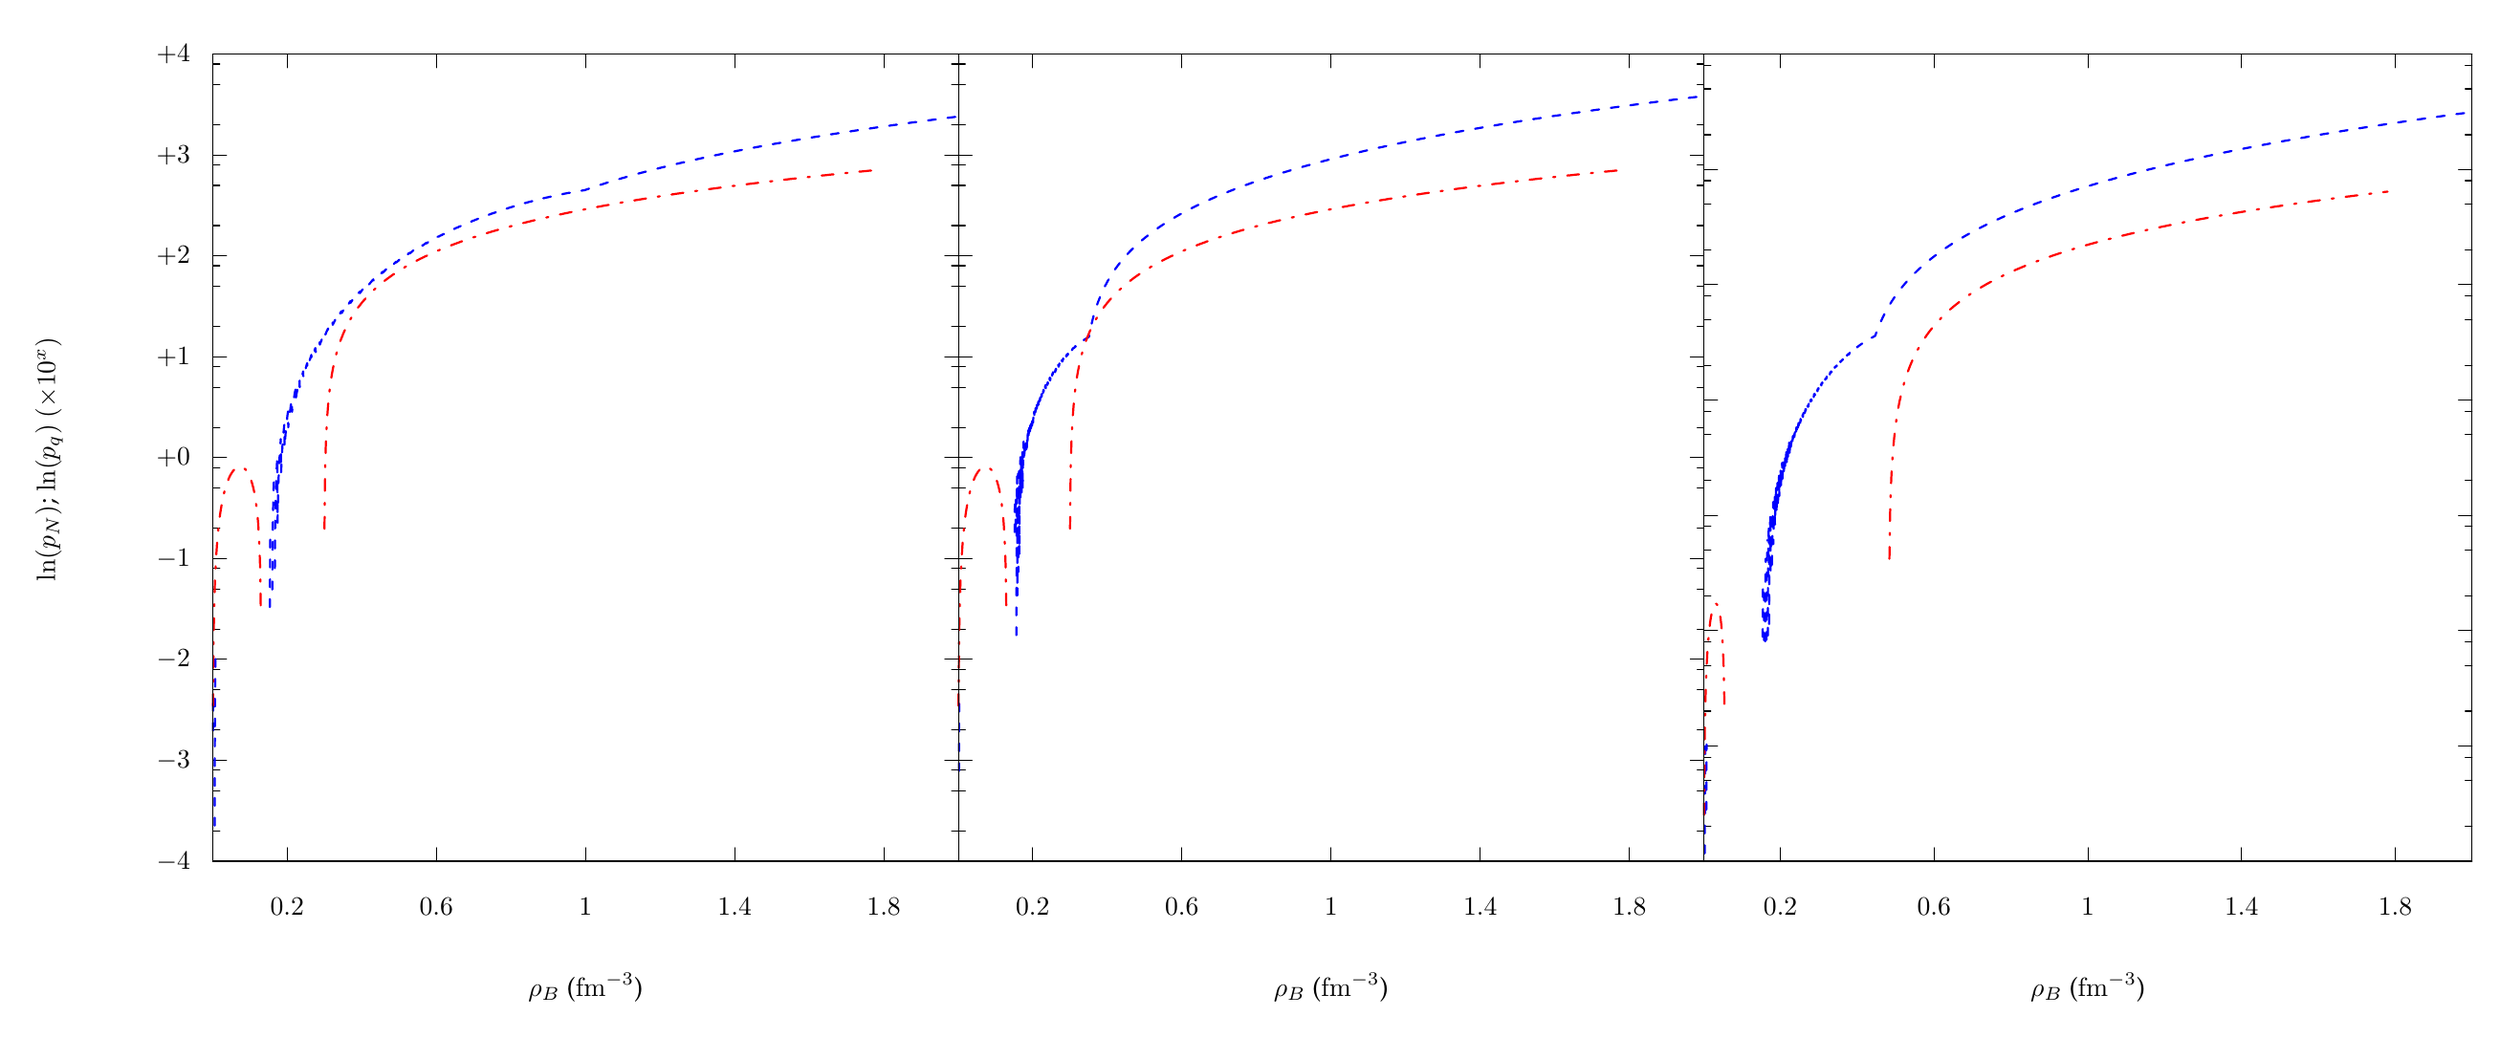
\begin{tikzpicture}[gnuplot]
%% generated with GNUPLOT 5.0p4 (Lua 5.2; terminal rev. 99, script rev. 100)
%% Wed Sep 28 20:03:24 2016
\path (0.000,0.000) rectangle (30.000,13.000);
\gpcolor{color=gp lt color border}
\gpsetlinetype{gp lt border}
\gpsetdashtype{gp dt solid}
\gpsetlinewidth{1.00}
\draw[gp path] (0.000,1.909)--(0.180,1.909);
\draw[gp path] (9.899,1.909)--(9.719,1.909);
\node[gp node right] at (-0.184,1.909) {$-4$};
\draw[gp path] (0.000,2.312)--(0.090,2.312);
\draw[gp path] (9.899,2.312)--(9.809,2.312);
\draw[gp path] (0.000,2.846)--(0.090,2.846);
\draw[gp path] (9.899,2.846)--(9.809,2.846);
\draw[gp path] (0.000,3.119)--(0.090,3.119);
\draw[gp path] (9.899,3.119)--(9.809,3.119);
\draw[gp path] (0.000,3.249)--(0.180,3.249);
\draw[gp path] (9.899,3.249)--(9.719,3.249);
\node[gp node right] at (-0.184,3.249) {$-3$};
\draw[gp path] (0.000,3.653)--(0.090,3.653);
\draw[gp path] (9.899,3.653)--(9.809,3.653);
\draw[gp path] (0.000,4.186)--(0.090,4.186);
\draw[gp path] (9.899,4.186)--(9.809,4.186);
\draw[gp path] (0.000,4.460)--(0.090,4.460);
\draw[gp path] (9.899,4.460)--(9.809,4.460);
\draw[gp path] (0.000,4.590)--(0.180,4.590);
\draw[gp path] (9.899,4.590)--(9.719,4.590);
\node[gp node right] at (-0.184,4.590) {$-2$};
\draw[gp path] (0.000,4.993)--(0.090,4.993);
\draw[gp path] (9.899,4.993)--(9.809,4.993);
\draw[gp path] (0.000,5.526)--(0.090,5.526);
\draw[gp path] (9.899,5.526)--(9.809,5.526);
\draw[gp path] (0.000,5.800)--(0.090,5.800);
\draw[gp path] (9.899,5.800)--(9.809,5.800);
\draw[gp path] (0.000,5.930)--(0.180,5.930);
\draw[gp path] (9.899,5.930)--(9.719,5.930);
\node[gp node right] at (-0.184,5.930) {$-1$};
\draw[gp path] (0.000,6.333)--(0.090,6.333);
\draw[gp path] (9.899,6.333)--(9.809,6.333);
\draw[gp path] (0.000,6.867)--(0.090,6.867);
\draw[gp path] (9.899,6.867)--(9.809,6.867);
\draw[gp path] (0.000,7.140)--(0.090,7.140);
\draw[gp path] (9.899,7.140)--(9.809,7.140);
\draw[gp path] (0.000,7.270)--(0.180,7.270);
\draw[gp path] (9.899,7.270)--(9.719,7.270);
\node[gp node right] at (-0.184,7.270) {$+0$};
\draw[gp path] (0.000,7.673)--(0.090,7.673);
\draw[gp path] (9.899,7.673)--(9.809,7.673);
\draw[gp path] (0.000,8.207)--(0.090,8.207);
\draw[gp path] (9.899,8.207)--(9.809,8.207);
\draw[gp path] (0.000,8.480)--(0.090,8.480);
\draw[gp path] (9.899,8.480)--(9.809,8.480);
\draw[gp path] (0.000,8.610)--(0.180,8.610);
\draw[gp path] (9.899,8.610)--(9.719,8.610);
\node[gp node right] at (-0.184,8.610) {$+1$};
\draw[gp path] (0.000,9.014)--(0.090,9.014);
\draw[gp path] (9.899,9.014)--(9.809,9.014);
\draw[gp path] (0.000,9.547)--(0.090,9.547);
\draw[gp path] (9.899,9.547)--(9.809,9.547);
\draw[gp path] (0.000,9.821)--(0.090,9.821);
\draw[gp path] (9.899,9.821)--(9.809,9.821);
\draw[gp path] (0.000,9.951)--(0.180,9.951);
\draw[gp path] (9.899,9.951)--(9.719,9.951);
\node[gp node right] at (-0.184,9.951) {$+2$};
\draw[gp path] (0.000,10.354)--(0.090,10.354);
\draw[gp path] (9.899,10.354)--(9.809,10.354);
\draw[gp path] (0.000,10.887)--(0.090,10.887);
\draw[gp path] (9.899,10.887)--(9.809,10.887);
\draw[gp path] (0.000,11.161)--(0.090,11.161);
\draw[gp path] (9.899,11.161)--(9.809,11.161);
\draw[gp path] (0.000,11.291)--(0.180,11.291);
\draw[gp path] (9.899,11.291)--(9.719,11.291);
\node[gp node right] at (-0.184,11.291) {$+3$};
\draw[gp path] (0.000,11.694)--(0.090,11.694);
\draw[gp path] (9.899,11.694)--(9.809,11.694);
\draw[gp path] (0.000,12.228)--(0.090,12.228);
\draw[gp path] (9.899,12.228)--(9.809,12.228);
\draw[gp path] (0.000,12.501)--(0.090,12.501);
\draw[gp path] (9.899,12.501)--(9.809,12.501);
\draw[gp path] (0.000,12.631)--(0.180,12.631);
\draw[gp path] (9.899,12.631)--(9.719,12.631);
\node[gp node right] at (-0.184,12.631) {$+4$};
\draw[gp path] (0.985,1.909)--(0.985,2.089);
\draw[gp path] (0.985,12.631)--(0.985,12.451);
\node[gp node center] at (0.985,1.293) {$0.2$};
\draw[gp path] (2.966,1.909)--(2.966,2.089);
\draw[gp path] (2.966,12.631)--(2.966,12.451);
\node[gp node center] at (2.966,1.293) {$0.6$};
\draw[gp path] (4.947,1.909)--(4.947,2.089);
\draw[gp path] (4.947,12.631)--(4.947,12.451);
\node[gp node center] at (4.947,1.293) {$1$};
\draw[gp path] (6.928,1.909)--(6.928,2.089);
\draw[gp path] (6.928,12.631)--(6.928,12.451);
\node[gp node center] at (6.928,1.293) {$1.4$};
\draw[gp path] (8.909,1.909)--(8.909,2.089);
\draw[gp path] (8.909,12.631)--(8.909,12.451);
\node[gp node center] at (8.909,1.293) {$1.8$};
\draw[gp path] (0.000,12.631)--(0.000,1.909)--(9.899,1.909)--(9.899,12.631)--cycle;
\node[gp node center,rotate=-270] at (-2.178,7.270) {$\ln(p_N)$; $\ln(p_q)$ $(\times 10^x)$};
\node[gp node center] at (4.949,0.215) {$\rho_B$ ($\rm{fm}^{-3}$)};
\gpcolor{rgb color={0.000,0.000,1.000}}
\gpsetdashtype{gp dt 3}
\gpsetlinewidth{2.00}
\draw[gp path] (0.000,3.641)--(0.003,4.085);
\draw[gp path] (0.023,2.381)--(0.026,3.906)--(0.030,4.338)--(0.033,4.613);
\draw[gp path] (0.756,5.285)--(0.759,6.008)--(0.762,6.323);
\draw[gp path] (0.789,5.519)--(0.792,6.106)--(0.795,6.394)--(0.799,6.587)--(0.802,6.733)%
  --(0.805,6.850)--(0.809,6.949);
\draw[gp path] (0.822,5.802)--(0.825,6.242)--(0.828,6.491)--(0.832,6.666)--(0.835,6.802)%
  --(0.838,6.912)--(0.842,7.006)--(0.845,7.087)--(0.848,7.159)--(0.852,7.223)--(0.855,7.281)%
  --(0.858,6.396)--(0.862,6.605)--(0.865,6.760)--(0.868,6.882)--(0.871,6.984)--(0.875,7.072)%
  --(0.878,7.148)--(0.881,7.216)--(0.885,7.278)--(0.888,7.334)--(0.891,7.385)--(0.895,7.433)%
  --(0.898,7.477)--(0.901,7.518)--(0.904,7.064)--(0.908,7.144)--(0.911,7.216)--(0.914,7.280)%
  --(0.918,7.338)--(0.921,7.391)--(0.924,7.440)--(0.928,7.485)--(0.931,7.527)--(0.934,7.567)%
  --(0.937,7.605)--(0.941,7.640)--(0.944,7.674)--(0.947,7.706)--(0.951,7.401)--(0.954,7.451)%
  --(0.957,7.498)--(0.961,7.541)--(0.964,7.581)--(0.967,7.619)--(0.970,7.655)--(0.974,7.689)%
  --(0.977,7.722)--(0.980,7.753)--(0.984,7.782)--(0.987,7.811)--(0.990,7.838)--(0.994,7.864)%
  --(0.997,7.889)--(1.000,7.674)--(1.003,7.708)--(1.007,7.741)--(1.010,7.772)--(1.013,7.801)%
  --(1.017,7.830)--(1.020,7.857)--(1.023,7.883)--(1.027,7.908)--(1.030,7.933)--(1.033,7.956)%
  --(1.036,7.979)--(1.040,8.001)--(1.043,8.022)--(1.046,8.043)--(1.050,7.879)--(1.053,7.905)%
  --(1.056,7.930)--(1.060,7.954)--(1.063,7.978)--(1.066,8.000)--(1.069,8.022)--(1.073,8.044)%
  --(1.076,8.064)--(1.079,8.084)--(1.083,8.104)--(1.086,8.123)--(1.089,8.141)--(1.093,8.159)%
  --(1.096,8.177)--(1.099,8.045)--(1.102,8.067)--(1.106,8.087)--(1.109,8.107)--(1.112,8.127)%
  --(1.116,8.145)--(1.119,8.164)--(1.122,8.182)--(1.126,8.199)--(1.129,8.216)--(1.132,8.233)%
  --(1.135,8.249)--(1.139,8.265)--(1.142,8.281)--(1.145,8.296)--(1.149,8.311)--(1.152,8.206)%
  --(1.155,8.223)--(1.159,8.240)--(1.162,8.256)--(1.165,8.273)--(1.168,8.288)--(1.172,8.304)%
  --(1.175,8.319)--(1.178,8.334)--(1.182,8.348)--(1.185,8.363)--(1.188,8.377)--(1.192,8.390)%
  --(1.195,8.404)--(1.198,8.417)--(1.201,8.328)--(1.205,8.343)--(1.208,8.358)--(1.211,8.372)%
  --(1.215,8.386)--(1.218,8.400)--(1.221,8.414)--(1.225,8.427)--(1.228,8.440)--(1.231,8.453)%
  --(1.234,8.466)--(1.238,8.478)--(1.241,8.491)--(1.244,8.503)--(1.248,8.515)--(1.251,8.526)%
  --(1.254,8.451)--(1.258,8.464)--(1.261,8.477)--(1.264,8.489)--(1.267,8.502)--(1.271,8.514)%
  --(1.274,8.526)--(1.277,8.538)--(1.281,8.549)--(1.284,8.561)--(1.287,8.572)--(1.291,8.583)%
  --(1.294,8.594)--(1.297,8.605)--(1.301,8.615)--(1.304,8.626)--(1.307,8.636)--(1.310,8.573)%
  --(1.314,8.584)--(1.317,8.595)--(1.320,8.606)--(1.324,8.617)--(1.327,8.628)--(1.330,8.638)%
  --(1.334,8.649)--(1.337,8.659)--(1.340,8.669)--(1.343,8.679)--(1.347,8.689)--(1.350,8.699)%
  --(1.353,8.708)--(1.357,8.718)--(1.360,8.727)--(1.363,8.672)--(1.367,8.682)--(1.370,8.692)%
  --(1.373,8.702)--(1.376,8.711)--(1.380,8.721)--(1.383,8.731)--(1.386,8.740)--(1.390,8.749)%
  --(1.393,8.758)--(1.396,8.768)--(1.400,8.777)--(1.403,8.785)--(1.406,8.794)--(1.409,8.803)%
  --(1.413,8.812)--(1.416,8.820)--(1.419,8.772)--(1.423,8.781)--(1.426,8.790)--(1.429,8.799)%
  --(1.433,8.808)--(1.436,8.816)--(1.439,8.825)--(1.442,8.833)--(1.446,8.842)--(1.449,8.850)%
  --(1.452,8.858)--(1.456,8.867)--(1.459,8.875)--(1.462,8.883)--(1.466,8.891)--(1.469,8.898)%
  --(1.472,8.906)--(1.475,8.864)--(1.479,8.872)--(1.482,8.880)--(1.485,8.888)--(1.489,8.896)%
  --(1.492,8.904)--(1.495,8.912)--(1.499,8.920)--(1.502,8.927)--(1.505,8.935)--(1.508,8.943)%
  --(1.512,8.950)--(1.515,8.958)--(1.518,8.965)--(1.522,8.972)--(1.525,8.979)--(1.528,8.987)%
  --(1.532,8.949)--(1.535,8.956)--(1.538,8.964)--(1.541,8.971)--(1.545,8.979)--(1.548,8.986)%
  --(1.551,8.993)--(1.555,9.000)--(1.558,9.007)--(1.561,9.014)--(1.565,9.021)--(1.568,9.028)%
  --(1.571,9.035)--(1.574,9.042)--(1.578,9.049)--(1.581,9.055)--(1.584,9.062)--(1.588,9.069)%
  --(1.591,9.035)--(1.594,9.042)--(1.598,9.049)--(1.601,9.056)--(1.604,9.062)--(1.607,9.069)%
  --(1.611,9.076)--(1.614,9.082)--(1.617,9.089)--(1.621,9.095)--(1.624,9.102)--(1.627,9.108)%
  --(1.631,9.114)--(1.634,9.121)--(1.637,9.127)--(1.640,9.133)--(1.644,9.139)--(1.647,9.145)%
  --(1.650,9.116)--(1.654,9.122)--(1.657,9.128)--(1.660,9.134)--(1.664,9.141)--(1.667,9.147)%
  --(1.670,9.153)--(1.673,9.159)--(1.677,9.165)--(1.680,9.171)--(1.683,9.177)--(1.687,9.183)%
  --(1.690,9.189)--(1.693,9.195)--(1.697,9.200)--(1.700,9.206)--(1.703,9.212)--(1.706,9.217)%
  --(1.710,9.191)--(1.713,9.197)--(1.716,9.202)--(1.720,9.208)--(1.723,9.214)--(1.726,9.220)%
  --(1.730,9.225)--(1.733,9.231)--(1.736,9.237)--(1.740,9.242)--(1.743,9.248)--(1.746,9.253)%
  --(1.749,9.259)--(1.753,9.264)--(1.756,9.270)--(1.759,9.275)--(1.763,9.280)--(1.766,9.286)%
  --(1.769,9.261)--(1.773,9.267)--(1.776,9.272)--(1.779,9.278)--(1.782,9.283)--(1.786,9.289)%
  --(1.789,9.294)--(1.792,9.299)--(1.796,9.304)--(1.799,9.310)--(1.802,9.315)--(1.806,9.320)%
  --(1.809,9.325)--(1.812,9.330)--(1.815,9.335)--(1.819,9.340)--(1.822,9.345)--(1.825,9.350)%
  --(1.829,9.328)--(1.832,9.333)--(1.835,9.338)--(1.839,9.344)--(1.842,9.349)--(1.845,9.354)%
  --(1.848,9.359)--(1.852,9.364)--(1.855,9.368)--(1.858,9.373)--(1.862,9.378)--(1.865,9.383)%
  --(1.868,9.388)--(1.872,9.393)--(1.875,9.398)--(1.878,9.402)--(1.881,9.407)--(1.885,9.412)%
  --(1.888,9.392)--(1.891,9.396)--(1.895,9.401)--(1.898,9.406)--(1.901,9.411)--(1.905,9.415)%
  --(1.908,9.420)--(1.911,9.425)--(1.914,9.429)--(1.918,9.434)--(1.921,9.439)--(1.924,9.443)%
  --(1.928,9.448)--(1.931,9.452)--(1.934,9.457)--(1.938,9.461)--(1.941,9.466)--(1.944,9.470)%
  --(1.947,9.475)--(1.951,9.456)--(1.954,9.461)--(1.957,9.465)--(1.961,9.470)--(1.964,9.474)%
  --(1.967,9.479)--(1.971,9.483)--(1.974,9.488)--(1.977,9.492)--(1.980,9.496)--(1.984,9.501)%
  --(1.987,9.505)--(1.990,9.509)--(1.994,9.514)--(1.997,9.518)--(2.000,9.522)--(2.004,9.526)%
  --(2.007,9.530)--(2.010,9.514)--(2.013,9.518)--(2.017,9.522)--(2.020,9.526)--(2.023,9.531)%
  --(2.027,9.535)--(2.030,9.539)--(2.033,9.543)--(2.037,9.547)--(2.040,9.551)--(2.043,9.556)%
  --(2.046,9.560)--(2.050,9.564)--(2.053,9.568)--(2.056,9.572)--(2.060,9.576)--(2.063,9.580)%
  --(2.066,9.584)--(2.070,9.588)--(2.073,9.572)--(2.076,9.576)--(2.079,9.580)--(2.083,9.584)%
  --(2.086,9.588)--(2.089,9.592)--(2.093,9.596)--(2.096,9.600)--(2.099,9.604)--(2.103,9.608)%
  --(2.106,9.612)--(2.109,9.616)--(2.112,9.620)--(2.116,9.624)--(2.119,9.628)--(2.122,9.631)%
  --(2.126,9.635)--(2.129,9.639)--(2.132,9.625)--(2.136,9.628)--(2.139,9.632)--(2.142,9.636)%
  --(2.145,9.640)--(2.149,9.644)--(2.152,9.647)--(2.155,9.651)--(2.159,9.655)--(2.162,9.659)%
  --(2.165,9.662)--(2.169,9.666)--(2.172,9.670)--(2.175,9.673)--(2.179,9.677)--(2.182,9.681)%
  --(2.185,9.684)--(2.188,9.688)--(2.192,9.692)--(2.195,9.678)--(2.198,9.682)--(2.202,9.686)%
  --(2.205,9.689)--(2.208,9.693)--(2.212,9.697)--(2.215,9.700)--(2.218,9.704)--(2.221,9.707)%
  --(2.225,9.711)--(2.228,9.714)--(2.231,9.718)--(2.235,9.721)--(2.238,9.725)--(2.241,9.728)%
  --(2.245,9.732)--(2.248,9.735)--(2.251,9.739)--(2.254,9.726)--(2.258,9.730)--(2.261,9.733)%
  --(2.264,9.737)--(2.268,9.740)--(2.271,9.744)--(2.274,9.747)--(2.278,9.751)--(2.281,9.754)%
  --(2.284,9.757)--(2.287,9.761)--(2.291,9.764)--(2.294,9.768)--(2.297,9.771)--(2.301,9.774)%
  --(2.304,9.778)--(2.307,9.781)--(2.311,9.784)--(2.314,9.788)--(2.317,9.776)--(2.320,9.779)%
  --(2.324,9.783)--(2.327,9.786)--(2.330,9.789)--(2.334,9.793)--(2.337,9.796)--(2.340,9.799)%
  --(2.344,9.802)--(2.347,9.806)--(2.350,9.809)--(2.353,9.812)--(2.357,9.815)--(2.360,9.819)%
  --(2.363,9.822)--(2.367,9.825)--(2.370,9.828)--(2.373,9.831)--(2.377,9.821)--(2.380,9.824)%
  --(2.383,9.827)--(2.386,9.830)--(2.390,9.833)--(2.393,9.836)--(2.396,9.840)--(2.400,9.843)%
  --(2.403,9.846)--(2.406,9.849)--(2.410,9.852)--(2.413,9.855)--(2.416,9.858)--(2.419,9.861)%
  --(2.423,9.865)--(2.426,9.868)--(2.429,9.871)--(2.433,9.874)--(2.436,9.864)--(2.439,9.867)%
  --(2.443,9.870)--(2.446,9.873)--(2.449,9.876)--(2.452,9.879)--(2.456,9.882)--(2.459,9.885)%
  --(2.462,9.888)--(2.466,9.891)--(2.469,9.894)--(2.472,9.897)--(2.476,9.900)--(2.479,9.903)%
  --(2.482,9.906)--(2.485,9.909)--(2.489,9.912)--(2.492,9.915)--(2.495,9.905)--(2.499,9.908)%
  --(2.502,9.911)--(2.505,9.914)--(2.509,9.917)--(2.512,9.920)--(2.515,9.923)--(2.518,9.926)%
  --(2.522,9.929)--(2.525,9.932)--(2.528,9.934)--(2.532,9.937)--(2.535,9.940)--(2.538,9.943)%
  --(2.542,9.946)--(2.545,9.949)--(2.548,9.952)--(2.551,9.954)--(2.555,9.945)--(2.558,9.948)%
  --(2.561,9.951)--(2.565,9.954)--(2.568,9.957)--(2.571,9.960)--(2.575,9.962)--(2.578,9.965)%
  --(2.581,9.968)--(2.585,9.971)--(2.588,9.974)--(2.591,9.976)--(2.594,9.979)--(2.598,9.982)%
  --(2.601,9.985)--(2.604,9.987)--(2.608,9.990)--(2.611,9.993)--(2.614,9.984)--(2.618,9.987)%
  --(2.621,9.990)--(2.624,9.993)--(2.627,9.995)--(2.631,9.998)--(2.634,10.001)--(2.637,10.003)%
  --(2.641,10.006)--(2.644,10.009)--(2.647,10.012)--(2.651,10.014)--(2.654,10.017)--(2.657,10.020)%
  --(2.660,10.022)--(2.664,10.025)--(2.667,10.028)--(2.670,10.019)--(2.674,10.022)--(2.677,10.025)%
  --(2.680,10.027)--(2.684,10.030)--(2.687,10.033)--(2.690,10.035)--(2.693,10.038)--(2.697,10.041)%
  --(2.700,10.043)--(2.703,10.046)--(2.707,10.048)--(2.710,10.051)--(2.713,10.054)--(2.717,10.056)%
  --(2.720,10.059)--(2.723,10.061)--(2.726,10.054)--(2.730,10.056)--(2.733,10.059)--(2.736,10.061)%
  --(2.740,10.064)--(2.743,10.067)--(2.746,10.069)--(2.750,10.072)--(2.753,10.074)--(2.756,10.077)%
  --(2.759,10.079)--(2.763,10.082)--(2.766,10.084)--(2.769,10.087)--(2.773,10.089)--(2.776,10.092)%
  --(2.779,10.094)--(2.783,10.087)--(2.786,10.090)--(2.789,10.092)--(2.792,10.094)--(2.796,10.097)%
  --(2.799,10.099)--(2.802,10.102)--(2.806,10.104)--(2.809,10.107)--(2.812,10.109)--(2.816,10.112)%
  --(2.819,10.114)--(2.822,10.117)--(2.825,10.119)--(2.829,10.122)--(2.832,10.124)--(2.835,10.117)%
  --(2.839,10.119)--(2.842,10.122)--(2.845,10.124)--(2.849,10.127)--(2.852,10.129)--(2.855,10.132)%
  --(2.858,10.134)--(2.862,10.136)--(2.865,10.139)--(2.868,10.141)--(2.872,10.144)--(2.875,10.146)%
  --(2.878,10.148)--(2.882,10.151)--(2.885,10.153)--(2.888,10.146)--(2.891,10.149)--(2.895,10.151)%
  --(2.898,10.153)--(2.901,10.156)--(2.905,10.158)--(2.908,10.160)--(2.911,10.163)--(2.915,10.165)%
  --(2.918,10.167)--(2.921,10.170)--(2.924,10.172)--(2.928,10.174)--(2.931,10.177)--(2.934,10.179)%
  --(2.938,10.181)--(2.941,10.175)--(2.944,10.177)--(2.948,10.180)--(2.951,10.182)--(2.954,10.184)%
  --(2.957,10.186)--(2.961,10.189)--(2.964,10.191)--(2.967,10.193)--(2.971,10.196)--(2.974,10.198)%
  --(2.977,10.200)--(2.981,10.202)--(2.984,10.205)--(2.987,10.207)--(2.990,10.209)--(2.994,10.205)%
  --(2.997,10.207)--(3.000,10.210)--(3.004,10.212)--(3.007,10.214)--(3.010,10.216)--(3.014,10.219)%
  --(3.017,10.217)--(3.020,10.219)--(3.024,10.221)--(3.027,10.223)--(3.030,10.225)--(3.033,10.228)%
  --(3.037,10.230)--(3.040,10.232)--(3.043,10.230)--(3.047,10.232)--(3.050,10.235)--(3.053,10.237)%
  --(3.057,10.239)--(3.060,10.241)--(3.063,10.243)--(3.066,10.242)--(3.070,10.244)--(3.073,10.246)%
  --(3.076,10.248)--(3.080,10.250)--(3.083,10.252)--(3.086,10.255)--(3.090,10.257)--(3.093,10.255)%
  --(3.096,10.257)--(3.099,10.259)--(3.103,10.261)--(3.106,10.263)--(3.109,10.266)--(3.113,10.268)%
  --(3.116,10.266)--(3.119,10.268)--(3.123,10.270)--(3.126,10.272)--(3.129,10.274)--(3.132,10.277)%
  --(3.136,10.279)--(3.139,10.277)--(3.142,10.279)--(3.146,10.281)--(3.149,10.283)--(3.152,10.285)%
  --(3.156,10.287)--(3.159,10.290)--(3.162,10.292)--(3.165,10.290)--(3.169,10.292)--(3.172,10.294)%
  --(3.175,10.296)--(3.179,10.298)--(3.182,10.300)--(3.185,10.302)--(3.189,10.301)--(3.192,10.303)%
  --(3.195,10.305)--(3.198,10.307)--(3.202,10.309)--(3.205,10.311)--(3.208,10.313)--(3.212,10.311)%
  --(3.215,10.314)--(3.218,10.316)--(3.222,10.318)--(3.225,10.320)--(3.228,10.322)--(3.231,10.324)%
  --(3.235,10.322)--(3.238,10.324)--(3.241,10.326)--(3.245,10.328)--(3.248,10.330)--(3.251,10.332)%
  --(3.255,10.331)--(3.258,10.333)--(3.261,10.335)--(3.264,10.337)--(3.268,10.339)--(3.271,10.341)%
  --(3.274,10.343)--(3.278,10.341)--(3.281,10.343)--(3.284,10.345)--(3.288,10.347)--(3.291,10.349)%
  --(3.294,10.351)--(3.297,10.353)--(3.301,10.352)--(3.304,10.353)--(3.307,10.355)--(3.311,10.357)%
  --(3.314,10.359)--(3.317,10.361)--(3.321,10.363)--(3.324,10.362)--(3.327,10.364)--(3.330,10.366)%
  --(3.334,10.368)--(3.337,10.370)--(3.340,10.371)--(3.344,10.370)--(3.347,10.372)--(3.350,10.374)%
  --(3.354,10.376)--(3.357,10.378)--(3.360,10.380)--(3.363,10.382)--(3.367,10.380)--(3.370,10.382)%
  --(3.373,10.384)--(3.377,10.386)--(3.380,10.388)--(3.383,10.390)--(3.387,10.388)--(3.390,10.390)%
  --(3.393,10.392)--(3.396,10.394)--(3.400,10.396)--(3.403,10.398)--(3.406,10.397)--(3.410,10.398)%
  --(3.413,10.400)--(3.416,10.402)--(3.420,10.404)--(3.423,10.406)--(3.426,10.408)--(3.429,10.407)%
  --(3.433,10.408)--(3.436,10.410)--(3.439,10.412)--(3.443,10.414)--(3.446,10.416)--(3.449,10.415)%
  --(3.453,10.416)--(3.456,10.418)--(3.459,10.420)--(3.463,10.422)--(3.466,10.424)--(3.469,10.423)%
  --(3.472,10.424)--(3.476,10.426)--(3.479,10.428)--(3.482,10.430)--(3.486,10.432)--(3.489,10.430)%
  --(3.492,10.432)--(3.496,10.434)--(3.499,10.436)--(3.502,10.438)--(3.505,10.440)--(3.509,10.438)%
  --(3.512,10.440)--(3.515,10.442)--(3.519,10.444)--(3.522,10.446)--(3.525,10.447)--(3.529,10.446)%
  --(3.532,10.448)--(3.535,10.450)--(3.538,10.452)--(3.542,10.453)--(3.545,10.455)--(3.548,10.454)%
  --(3.552,10.456)--(3.555,10.458)--(3.558,10.459)--(3.562,10.461)--(3.565,10.463)--(3.568,10.462)%
  --(3.571,10.463)--(3.575,10.465)--(3.578,10.467)--(3.581,10.469)--(3.585,10.468)--(3.588,10.469)%
  --(3.591,10.471)--(3.595,10.473)--(3.598,10.475)--(3.601,10.476)--(3.604,10.475)--(3.608,10.477)%
  --(3.611,10.479)--(3.614,10.481)--(3.618,10.482)--(3.621,10.484)--(3.624,10.483)--(3.628,10.485)%
  --(3.631,10.486)--(3.634,10.488)--(3.637,10.490)--(3.641,10.489)--(3.644,10.491)--(3.647,10.492)%
  --(3.651,10.494)--(3.654,10.496)--(3.657,10.497)--(3.661,10.496)--(3.664,10.498)--(3.667,10.500)%
  --(3.670,10.501)--(3.674,10.503)--(3.677,10.502)--(3.680,10.504)--(3.684,10.506)--(3.687,10.507)%
  --(3.690,10.509)--(3.694,10.511)--(3.697,10.510)--(3.700,10.511)--(3.703,10.513)--(3.707,10.515)%
  --(3.710,10.516)--(3.713,10.515)--(3.717,10.517)--(3.720,10.519)--(3.723,10.520)--(3.727,10.522)%
  --(3.730,10.521)--(3.733,10.523)--(3.736,10.524)--(3.740,10.526)--(3.743,10.528)--(3.746,10.527)%
  --(3.750,10.528)--(3.753,10.530)--(3.756,10.532)--(3.760,10.533)--(3.763,10.532)--(3.766,10.534)%
  --(3.769,10.536)--(3.773,10.537)--(3.776,10.539)--(3.779,10.538)--(3.783,10.540)--(3.786,10.541)%
  --(3.789,10.543)--(3.793,10.545)--(3.796,10.544)--(3.799,10.545)--(3.802,10.547)--(3.806,10.549)%
  --(3.809,10.550)--(3.812,10.549)--(3.816,10.551)--(3.819,10.553)--(3.822,10.554)--(3.826,10.556)%
  --(3.829,10.555)--(3.832,10.557)--(3.835,10.558)--(3.839,10.560)--(3.842,10.561)--(3.845,10.561)%
  --(3.849,10.562)--(3.852,10.564)--(3.855,10.565)--(3.859,10.567)--(3.862,10.566)--(3.865,10.568)%
  --(3.868,10.569)--(3.872,10.571)--(3.875,10.573)--(3.878,10.572)--(3.882,10.573)--(3.885,10.575)%
  --(3.888,10.576)--(3.892,10.576)--(3.895,10.577)--(3.898,10.579)--(3.902,10.580)--(3.905,10.582)%
  --(3.908,10.581)--(3.911,10.583)--(3.915,10.584)--(3.918,10.586)--(3.921,10.587)--(3.925,10.587)%
  --(3.928,10.588)--(3.931,10.590)--(3.935,10.591)--(3.938,10.591)--(3.941,10.592)--(3.944,10.594)%
  --(3.948,10.595)--(3.951,10.597)--(3.954,10.596)--(3.958,10.598)--(3.961,10.599)--(3.964,10.601)%
  --(3.968,10.600)--(3.971,10.601)--(3.974,10.603)--(3.977,10.604)--(3.981,10.604)--(3.984,10.605)%
  --(3.987,10.607)--(3.991,10.608)--(3.994,10.610)--(3.997,10.609)--(4.001,10.611)--(4.004,10.612)%
  --(4.007,10.614)--(4.010,10.613)--(4.014,10.615)--(4.017,10.616)--(4.020,10.618)--(4.024,10.617)%
  --(4.027,10.618)--(4.030,10.620)--(4.034,10.621)--(4.037,10.623)--(4.040,10.622)--(4.043,10.624)%
  --(4.047,10.625)--(4.050,10.627)--(4.053,10.626)--(4.057,10.628)--(4.060,10.629)--(4.063,10.631)%
  --(4.067,10.630)--(4.070,10.631)--(4.073,10.633)--(4.076,10.634)--(4.080,10.634)--(4.083,10.635)%
  --(4.086,10.637)--(4.090,10.638)--(4.093,10.638)--(4.096,10.639)--(4.100,10.640)--(4.103,10.642)%
  --(4.106,10.641)--(4.109,10.643)--(4.113,10.644)--(4.116,10.646)--(4.119,10.645)--(4.123,10.647)%
  --(4.126,10.648)--(4.129,10.650)--(4.133,10.649)--(4.136,10.650)--(4.139,10.652)--(4.142,10.653)%
  --(4.146,10.653)--(4.149,10.654)--(4.152,10.656)--(4.156,10.655)--(4.159,10.657)--(4.162,10.658)%
  --(4.166,10.659)--(4.169,10.659)--(4.172,10.660)--(4.175,10.662)--(4.179,10.663)--(4.182,10.663)%
  --(4.185,10.664)--(4.189,10.666)--(4.192,10.667)--(4.195,10.666)--(4.199,10.668)--(4.202,10.669)%
  --(4.205,10.669)--(4.208,10.670)--(4.212,10.672)--(4.215,10.673)--(4.218,10.673)--(4.222,10.674)%
  --(4.225,10.675)--(4.228,10.675)--(4.232,10.676)--(4.235,10.678)--(4.238,10.679)--(4.241,10.679)%
  --(4.245,10.680)--(4.248,10.681)--(4.251,10.683)--(4.255,10.682)--(4.258,10.684)--(4.261,10.685)%
  --(4.265,10.685)--(4.268,10.686)--(4.271,10.688)--(4.274,10.687)--(4.278,10.688)--(4.281,10.690)%
  --(4.284,10.691)--(4.288,10.691)--(4.291,10.692)--(4.294,10.694)--(4.298,10.693)--(4.301,10.695)%
  --(4.304,10.696)--(4.308,10.696)--(4.311,10.697)--(4.314,10.698)--(4.317,10.700)--(4.321,10.699)%
  --(4.324,10.701)--(4.327,10.702)--(4.331,10.702)--(4.334,10.703)--(4.337,10.704)--(4.341,10.704)%
  --(4.344,10.705)--(4.347,10.707)--(4.350,10.706)--(4.354,10.708)--(4.357,10.709)--(4.360,10.710)%
  --(4.364,10.710)--(4.367,10.711)--(4.370,10.713)--(4.374,10.712)--(4.377,10.714)--(4.380,10.715)%
  --(4.383,10.715)--(4.387,10.716)--(4.390,10.717)--(4.393,10.717)--(4.397,10.719)--(4.400,10.720)%
  --(4.403,10.720)--(4.407,10.721)--(4.410,10.722)--(4.413,10.722)--(4.416,10.723)--(4.420,10.725)%
  --(4.423,10.724)--(4.426,10.726)--(4.430,10.727)--(4.433,10.727)--(4.436,10.728)--(4.440,10.728)%
  --(4.443,10.729)--(4.446,10.730)--(4.449,10.730)--(4.453,10.731)--(4.456,10.733)--(4.459,10.732)%
  --(4.463,10.734)--(4.466,10.735)--(4.469,10.735)--(4.473,10.736)--(4.476,10.738)--(4.479,10.737)%
  --(4.482,10.739)--(4.486,10.738)--(4.489,10.740)--(4.492,10.741)--(4.496,10.741)--(4.499,10.742)%
  --(4.502,10.743)--(4.506,10.743)--(4.509,10.745)--(4.512,10.744)--(4.515,10.746)--(4.519,10.747)%
  --(4.522,10.747)--(4.525,10.748)--(4.529,10.749)--(4.532,10.750)--(4.535,10.750)--(4.539,10.751)%
  --(4.542,10.751)--(4.545,10.753)--(4.548,10.753)--(4.552,10.754)--(4.555,10.754)--(4.558,10.755)%
  --(4.562,10.755)--(4.565,10.757)--(4.568,10.757)--(4.572,10.758)--(4.575,10.758)--(4.578,10.759)%
  --(4.581,10.760)--(4.585,10.761)--(4.588,10.761)--(4.591,10.762)--(4.595,10.763)--(4.598,10.763)%
  --(4.601,10.764)--(4.605,10.764)--(4.608,10.766)--(4.611,10.766)--(4.614,10.767)--(4.618,10.768)%
  --(4.621,10.768)--(4.624,10.769)--(4.628,10.769)--(4.631,10.770)--(4.634,10.771)--(4.638,10.771)%
  --(4.641,10.772)--(4.644,10.773)--(4.647,10.774)--(4.651,10.774)--(4.654,10.775)--(4.657,10.776)%
  --(4.661,10.776)--(4.664,10.777)--(4.667,10.778)--(4.671,10.778)--(4.674,10.779)--(4.677,10.779)%
  --(4.680,10.780)--(4.684,10.781)--(4.687,10.781)--(4.690,10.782)--(4.694,10.783)--(4.697,10.783)%
  --(4.700,10.784)--(4.704,10.785)--(4.707,10.785)--(4.710,10.785)--(4.713,10.786)--(4.717,10.787)%
  --(4.720,10.788)--(4.723,10.788)--(4.727,10.789)--(4.730,10.790)--(4.733,10.790)--(4.737,10.790)%
  --(4.740,10.791)--(4.743,10.792)--(4.747,10.793)--(4.750,10.793)--(4.753,10.794)--(4.756,10.794)%
  --(4.760,10.795)--(4.763,10.796)--(4.766,10.796)--(4.770,10.797)--(4.773,10.797)--(4.776,10.798)%
  --(4.780,10.798)--(4.783,10.799)--(4.786,10.800)--(4.789,10.800)--(4.793,10.801)--(4.796,10.802)%
  --(4.799,10.802)--(4.803,10.803)--(4.806,10.803)--(4.809,10.804)--(4.813,10.804)--(4.816,10.805)%
  --(4.819,10.806)--(4.822,10.806)--(4.826,10.806)--(4.829,10.807)--(4.832,10.808)--(4.836,10.808)%
  --(4.839,10.809)--(4.842,10.809)--(4.846,10.810)--(4.849,10.810)--(4.852,10.811)--(4.855,10.812)%
  --(4.859,10.812)--(4.862,10.813)--(4.865,10.813)--(4.869,10.814)--(4.872,10.814)--(4.875,10.815)%
  --(4.879,10.815)--(4.882,10.816)--(4.885,10.817)--(4.888,10.817)--(4.892,10.818)--(4.895,10.818)%
  --(4.898,10.819)--(4.902,10.819)--(4.905,10.820)--(4.908,10.820)--(4.912,10.821)--(4.915,10.821)%
  --(4.918,10.822)--(4.921,10.822)--(4.925,10.823)--(4.928,10.823)--(4.931,10.824)--(4.935,10.824)%
  --(4.938,10.825)--(4.941,10.827)--(4.945,10.828)--(4.948,10.829)--(4.951,10.830)--(4.954,10.831)%
  --(4.958,10.832)--(4.961,10.833)--(4.964,10.835)--(4.968,10.836)--(4.971,10.837)--(4.974,10.838)%
  --(4.978,10.839)--(4.981,10.840)--(4.984,10.841)--(4.987,10.843)--(4.991,10.844)--(4.994,10.845)%
  --(4.997,10.846)--(5.001,10.847)--(5.004,10.848)--(5.007,10.849)--(5.011,10.850)--(5.014,10.852)%
  --(5.017,10.853)--(5.020,10.854)--(5.024,10.855)--(5.027,10.856)--(5.030,10.857)--(5.034,10.858)%
  --(5.037,10.859)--(5.040,10.861)--(5.044,10.862)--(5.047,10.863)--(5.050,10.864)--(5.053,10.865)%
  --(5.057,10.866)--(5.060,10.867)--(5.063,10.868)--(5.067,10.869)--(5.070,10.871)--(5.073,10.872)%
  --(5.077,10.873)--(5.080,10.874)--(5.083,10.875)--(5.086,10.876)--(5.090,10.877)--(5.093,10.878)%
  --(5.096,10.879)--(5.100,10.880)--(5.103,10.881)--(5.106,10.883)--(5.110,10.884)--(5.113,10.885)%
  --(5.116,10.886)--(5.119,10.887)--(5.123,10.888)--(5.126,10.889)--(5.129,10.890)--(5.133,10.891)%
  --(5.136,10.892)--(5.139,10.893)--(5.143,10.894)--(5.146,10.895)--(5.149,10.896)--(5.152,10.898)%
  --(5.156,10.899)--(5.159,10.900)--(5.162,10.901)--(5.166,10.902)--(5.169,10.903)--(5.172,10.904)%
  --(5.176,10.905)--(5.179,10.906)--(5.182,10.907)--(5.186,10.908)--(5.189,10.909)--(5.192,10.910)%
  --(5.195,10.911)--(5.199,10.912)--(5.202,10.913)--(5.205,10.914)--(5.209,10.915)--(5.212,10.917)%
  --(5.215,10.918)--(5.219,10.919)--(5.222,10.920)--(5.225,10.921)--(5.228,10.922)--(5.232,10.923)%
  --(5.235,10.924)--(5.238,10.925)--(5.242,10.926)--(5.245,10.927)--(5.248,10.928)--(5.252,10.929)%
  --(5.255,10.930)--(5.258,10.931)--(5.261,10.932)--(5.265,10.933)--(5.268,10.934)--(5.271,10.935)%
  --(5.275,10.936)--(5.278,10.937)--(5.281,10.938)--(5.285,10.939)--(5.288,10.940)--(5.291,10.941)%
  --(5.294,10.942)--(5.298,10.943)--(5.301,10.944)--(5.304,10.945)--(5.308,10.946)--(5.311,10.947)%
  --(5.314,10.948)--(5.318,10.949)--(5.321,10.950)--(5.324,10.951)--(5.327,10.952)--(5.331,10.953)%
  --(5.334,10.954)--(5.337,10.955)--(5.341,10.956)--(5.344,10.957)--(5.347,10.958)--(5.351,10.959)%
  --(5.354,10.960)--(5.357,10.961)--(5.360,10.962)--(5.364,10.963)--(5.367,10.964)--(5.370,10.965)%
  --(5.374,10.966)--(5.377,10.967)--(5.380,10.968)--(5.384,10.969)--(5.387,10.970)--(5.390,10.971)%
  --(5.393,10.972)--(5.397,10.973)--(5.400,10.974)--(5.403,10.975)--(5.407,10.976)--(5.410,10.977)%
  --(5.413,10.978)--(5.417,10.979)--(5.420,10.980)--(5.423,10.981)--(5.426,10.982)--(5.430,10.983)%
  --(5.433,10.984)--(5.436,10.985)--(5.440,10.986)--(5.443,10.987)--(5.446,10.987)--(5.450,10.988)%
  --(5.453,10.989)--(5.456,10.990)--(5.459,10.991)--(5.463,10.992)--(5.466,10.993)--(5.469,10.994)%
  --(5.473,10.995)--(5.476,10.996)--(5.479,10.997)--(5.483,10.998)--(5.486,10.999)--(5.489,11.000)%
  --(5.492,11.001)--(5.496,11.002)--(5.499,11.003)--(5.502,11.004)--(5.506,11.005)--(5.509,11.006)%
  --(5.512,11.006)--(5.516,11.007)--(5.519,11.008)--(5.522,11.009)--(5.525,11.010)--(5.529,11.011)%
  --(5.532,11.012)--(5.535,11.013)--(5.539,11.014)--(5.542,11.015)--(5.545,11.016)--(5.549,11.017)%
  --(5.552,11.018)--(5.555,11.019)--(5.558,11.020)--(5.562,11.020)--(5.565,11.021)--(5.568,11.022)%
  --(5.572,11.023)--(5.575,11.024)--(5.578,11.025)--(5.582,11.026)--(5.585,11.027)--(5.588,11.028)%
  --(5.591,11.029)--(5.595,11.030)--(5.598,11.031)--(5.601,11.032)--(5.605,11.032)--(5.608,11.033)%
  --(5.611,11.034)--(5.615,11.035)--(5.618,11.036)--(5.621,11.037)--(5.625,11.038)--(5.628,11.039)%
  --(5.631,11.040)--(5.634,11.041)--(5.638,11.042)--(5.641,11.042)--(5.644,11.043)--(5.648,11.044)%
  --(5.651,11.045)--(5.654,11.046)--(5.658,11.047)--(5.661,11.048)--(5.664,11.049)--(5.667,11.050)%
  --(5.671,11.051)--(5.674,11.051)--(5.677,11.052)--(5.681,11.053)--(5.684,11.054)--(5.687,11.055)%
  --(5.691,11.056)--(5.694,11.057)--(5.697,11.058)--(5.700,11.059)--(5.704,11.059)--(5.707,11.060)%
  --(5.710,11.061)--(5.714,11.062)--(5.717,11.063)--(5.720,11.064)--(5.724,11.065)--(5.727,11.066)%
  --(5.730,11.066)--(5.733,11.067)--(5.737,11.068)--(5.740,11.069)--(5.743,11.070)--(5.747,11.071)%
  --(5.750,11.072)--(5.753,11.073)--(5.757,11.073)--(5.760,11.074)--(5.763,11.075)--(5.766,11.076)%
  --(5.770,11.077)--(5.773,11.078)--(5.776,11.079)--(5.780,11.080)--(5.783,11.080)--(5.786,11.081)%
  --(5.790,11.082)--(5.793,11.083)--(5.796,11.084)--(5.799,11.085)--(5.803,11.086)--(5.806,11.086)%
  --(5.809,11.087)--(5.813,11.088)--(5.816,11.089)--(5.819,11.090)--(5.823,11.091)--(5.826,11.092)%
  --(5.829,11.092)--(5.832,11.093)--(5.836,11.094)--(5.839,11.095)--(5.842,11.096)--(5.846,11.097)%
  --(5.849,11.098)--(5.852,11.098)--(5.856,11.099)--(5.859,11.100)--(5.862,11.101)--(5.865,11.102)%
  --(5.869,11.103)--(5.872,11.103)--(5.875,11.104)--(5.879,11.105)--(5.882,11.106)--(5.885,11.107)%
  --(5.889,11.108)--(5.892,11.109)--(5.895,11.109)--(5.898,11.110)--(5.902,11.111)--(5.905,11.112)%
  --(5.908,11.113)--(5.912,11.114)--(5.915,11.114)--(5.918,11.115)--(5.922,11.116)--(5.925,11.117)%
  --(5.928,11.118)--(5.931,11.119)--(5.935,11.119)--(5.938,11.120)--(5.941,11.121)--(5.945,11.122)%
  --(5.948,11.123)--(5.951,11.124)--(5.955,11.124)--(5.958,11.125)--(5.961,11.126)--(5.964,11.127)%
  --(5.968,11.128)--(5.971,11.128)--(5.974,11.129)--(5.978,11.130)--(5.981,11.131)--(5.984,11.132)%
  --(5.988,11.133)--(5.991,11.133)--(5.994,11.134)--(5.997,11.135)--(6.001,11.136)--(6.004,11.137)%
  --(6.007,11.137)--(6.011,11.138)--(6.014,11.139)--(6.017,11.140)--(6.021,11.141)--(6.024,11.141)%
  --(6.027,11.142)--(6.031,11.143)--(6.034,11.144)--(6.037,11.145)--(6.040,11.146)--(6.044,11.146)%
  --(6.047,11.147)--(6.050,11.148)--(6.054,11.149)--(6.057,11.150)--(6.060,11.150)--(6.064,11.151)%
  --(6.067,11.152)--(6.070,11.153)--(6.073,11.154)--(6.077,11.154)--(6.080,11.155)--(6.083,11.156)%
  --(6.087,11.157)--(6.090,11.158)--(6.093,11.158)--(6.097,11.159)--(6.100,11.160)--(6.103,11.161)%
  --(6.106,11.161)--(6.110,11.162)--(6.113,11.163)--(6.116,11.164)--(6.120,11.165)--(6.123,11.165)%
  --(6.126,11.166)--(6.130,11.167)--(6.133,11.168)--(6.136,11.169)--(6.139,11.169)--(6.143,11.170)%
  --(6.146,11.171)--(6.149,11.172)--(6.153,11.173)--(6.156,11.173)--(6.159,11.174)--(6.163,11.175)%
  --(6.166,11.176)--(6.169,11.176)--(6.172,11.177)--(6.176,11.178)--(6.179,11.179)--(6.182,11.180)%
  --(6.186,11.180)--(6.189,11.181)--(6.192,11.182)--(6.196,11.183)--(6.199,11.183)--(6.202,11.184)%
  --(6.205,11.185)--(6.209,11.186)--(6.212,11.186)--(6.215,11.187)--(6.219,11.188)--(6.222,11.189)%
  --(6.225,11.190)--(6.229,11.190)--(6.232,11.191)--(6.235,11.192)--(6.238,11.193)--(6.242,11.193)%
  --(6.245,11.194)--(6.248,11.195)--(6.252,11.196)--(6.255,11.196)--(6.258,11.197)--(6.262,11.198)%
  --(6.265,11.199)--(6.268,11.199)--(6.271,11.200)--(6.275,11.201)--(6.278,11.202)--(6.281,11.203)%
  --(6.285,11.203)--(6.288,11.204)--(6.291,11.205)--(6.295,11.206)--(6.298,11.206)--(6.301,11.207)%
  --(6.304,11.208)--(6.308,11.209)--(6.311,11.209)--(6.314,11.210)--(6.318,11.211)--(6.321,11.212)%
  --(6.324,11.212)--(6.328,11.213)--(6.331,11.214)--(6.334,11.215)--(6.337,11.215)--(6.341,11.216)%
  --(6.344,11.217)--(6.347,11.218)--(6.351,11.218)--(6.354,11.219)--(6.357,11.220)--(6.361,11.221)%
  --(6.364,11.221)--(6.367,11.222)--(6.370,11.223)--(6.374,11.224)--(6.377,11.224)--(6.380,11.225)%
  --(6.384,11.226)--(6.387,11.226)--(6.390,11.227)--(6.394,11.228)--(6.397,11.229)--(6.400,11.229)%
  --(6.403,11.230)--(6.407,11.231)--(6.410,11.232)--(6.413,11.232)--(6.417,11.233)--(6.420,11.234)%
  --(6.423,11.235)--(6.427,11.235)--(6.430,11.236)--(6.433,11.237)--(6.436,11.237)--(6.440,11.238)%
  --(6.443,11.239)--(6.446,11.240)--(6.450,11.240)--(6.453,11.241)--(6.456,11.242)--(6.460,11.243)%
  --(6.463,11.243)--(6.466,11.244)--(6.470,11.245)--(6.473,11.245)--(6.476,11.246)--(6.479,11.247)%
  --(6.483,11.248)--(6.486,11.248)--(6.489,11.249)--(6.493,11.250)--(6.496,11.251)--(6.499,11.251)%
  --(6.503,11.252)--(6.506,11.253)--(6.509,11.253)--(6.512,11.254)--(6.516,11.255)--(6.519,11.256)%
  --(6.522,11.256)--(6.526,11.257)--(6.529,11.258)--(6.532,11.258)--(6.536,11.259)--(6.539,11.260)%
  --(6.542,11.261)--(6.545,11.261)--(6.549,11.262)--(6.552,11.263)--(6.555,11.263)--(6.559,11.264)%
  --(6.562,11.265)--(6.565,11.266)--(6.569,11.266)--(6.572,11.267)--(6.575,11.268)--(6.578,11.268)%
  --(6.582,11.269)--(6.585,11.270)--(6.588,11.270)--(6.592,11.271)--(6.595,11.272)--(6.598,11.273)%
  --(6.602,11.273)--(6.605,11.274)--(6.608,11.275)--(6.611,11.275)--(6.615,11.276)--(6.618,11.277)%
  --(6.621,11.277)--(6.625,11.278)--(6.628,11.279)--(6.631,11.280)--(6.635,11.280)--(6.638,11.281)%
  --(6.641,11.282)--(6.644,11.282)--(6.648,11.283)--(6.651,11.284)--(6.654,11.284)--(6.658,11.285)%
  --(6.661,11.286)--(6.664,11.287)--(6.668,11.287)--(6.671,11.288)--(6.674,11.289)--(6.677,11.289)%
  --(6.681,11.290)--(6.684,11.291)--(6.687,11.291)--(6.691,11.292)--(6.694,11.293)--(6.697,11.293)%
  --(6.701,11.294)--(6.704,11.295)--(6.707,11.295)--(6.710,11.296)--(6.714,11.297)--(6.717,11.298)%
  --(6.720,11.298)--(6.724,11.299)--(6.727,11.300)--(6.730,11.300)--(6.734,11.301)--(6.737,11.302)%
  --(6.740,11.302)--(6.743,11.303)--(6.747,11.304)--(6.750,11.304)--(6.753,11.305)--(6.757,11.306)%
  --(6.760,11.306)--(6.763,11.307)--(6.767,11.308)--(6.770,11.308)--(6.773,11.309)--(6.776,11.310)%
  --(6.780,11.310)--(6.783,11.311)--(6.786,11.312)--(6.790,11.312)--(6.793,11.313)--(6.796,11.314)%
  --(6.800,11.315)--(6.803,11.315)--(6.806,11.316)--(6.809,11.317)--(6.813,11.317)--(6.816,11.318)%
  --(6.819,11.319)--(6.823,11.319)--(6.826,11.320)--(6.829,11.321)--(6.833,11.321)--(6.836,11.322)%
  --(6.839,11.323)--(6.842,11.323)--(6.846,11.324)--(6.849,11.325)--(6.852,11.325)--(6.856,11.326)%
  --(6.859,11.327)--(6.862,11.327)--(6.866,11.328)--(6.869,11.329)--(6.872,11.329)--(6.875,11.330)%
  --(6.879,11.331)--(6.882,11.331)--(6.885,11.332)--(6.889,11.333)--(6.892,11.333)--(6.895,11.334)%
  --(6.899,11.334)--(6.902,11.335)--(6.905,11.336)--(6.909,11.336)--(6.912,11.337)--(6.915,11.338)%
  --(6.918,11.338)--(6.922,11.339)--(6.925,11.340)--(6.928,11.340)--(6.932,11.341)--(6.935,11.342)%
  --(6.938,11.342)--(6.942,11.343)--(6.945,11.344)--(6.948,11.344)--(6.951,11.345)--(6.955,11.346)%
  --(6.958,11.346)--(6.961,11.347)--(6.965,11.348)--(6.968,11.348)--(6.971,11.349)--(6.975,11.350)%
  --(6.978,11.350)--(6.981,11.351)--(6.984,11.351)--(6.988,11.352)--(6.991,11.353)--(6.994,11.353)%
  --(6.998,11.354)--(7.001,11.355)--(7.004,11.355)--(7.008,11.356)--(7.011,11.357)--(7.014,11.357)%
  --(7.017,11.358)--(7.021,11.359)--(7.024,11.359)--(7.027,11.360)--(7.031,11.360)--(7.034,11.361)%
  --(7.037,11.362)--(7.041,11.362)--(7.044,11.363)--(7.047,11.364)--(7.050,11.364)--(7.054,11.365)%
  --(7.057,11.366)--(7.060,11.366)--(7.064,11.367)--(7.067,11.368)--(7.070,11.368)--(7.074,11.369)%
  --(7.077,11.369)--(7.080,11.370)--(7.083,11.371)--(7.087,11.371)--(7.090,11.372)--(7.093,11.373)%
  --(7.097,11.373)--(7.100,11.374)--(7.103,11.375)--(7.107,11.375)--(7.110,11.376)--(7.113,11.376)%
  --(7.116,11.377)--(7.120,11.378)--(7.123,11.378)--(7.126,11.379)--(7.130,11.380)--(7.133,11.380)%
  --(7.136,11.381)--(7.140,11.381)--(7.143,11.382)--(7.146,11.383)--(7.149,11.383)--(7.153,11.384)%
  --(7.156,11.385)--(7.159,11.385)--(7.163,11.386)--(7.166,11.386)--(7.169,11.387)--(7.173,11.388)%
  --(7.176,11.388)--(7.179,11.389)--(7.182,11.390)--(7.186,11.390)--(7.189,11.391)--(7.192,11.391)%
  --(7.196,11.392)--(7.199,11.393)--(7.202,11.393)--(7.206,11.394)--(7.209,11.395)--(7.212,11.395)%
  --(7.215,11.396)--(7.219,11.396)--(7.222,11.397)--(7.225,11.398)--(7.229,11.398)--(7.232,11.399)%
  --(7.235,11.399)--(7.239,11.400)--(7.242,11.401)--(7.245,11.401)--(7.248,11.402)--(7.252,11.403)%
  --(7.255,11.403)--(7.258,11.404)--(7.262,11.404)--(7.265,11.405)--(7.268,11.406)--(7.272,11.406)%
  --(7.275,11.407)--(7.278,11.407)--(7.281,11.408)--(7.285,11.409)--(7.288,11.409)--(7.291,11.410)%
  --(7.295,11.411)--(7.298,11.411)--(7.301,11.412)--(7.305,11.412)--(7.308,11.413)--(7.311,11.414)%
  --(7.314,11.414)--(7.318,11.415)--(7.321,11.415)--(7.324,11.416)--(7.328,11.417)--(7.331,11.417)%
  --(7.334,11.418)--(7.338,11.418)--(7.341,11.419)--(7.344,11.420)--(7.348,11.420)--(7.351,11.421)%
  --(7.354,11.421)--(7.357,11.422)--(7.361,11.423)--(7.364,11.423)--(7.367,11.424)--(7.371,11.424)%
  --(7.374,11.425)--(7.377,11.426)--(7.381,11.426)--(7.384,11.427)--(7.387,11.427)--(7.390,11.428)%
  --(7.394,11.429)--(7.397,11.429)--(7.400,11.430)--(7.404,11.430)--(7.407,11.431)--(7.410,11.432)%
  --(7.414,11.432)--(7.417,11.433)--(7.420,11.433)--(7.423,11.434)--(7.427,11.435)--(7.430,11.435)%
  --(7.433,11.436)--(7.437,11.436)--(7.440,11.437)--(7.443,11.438)--(7.447,11.438)--(7.450,11.439)%
  --(7.453,11.439)--(7.456,11.440)--(7.460,11.441)--(7.463,11.441)--(7.466,11.442)--(7.470,11.442)%
  --(7.473,11.443)--(7.476,11.443)--(7.480,11.444)--(7.483,11.445)--(7.486,11.445)--(7.489,11.446)%
  --(7.493,11.446)--(7.496,11.447)--(7.499,11.448)--(7.503,11.448)--(7.506,11.449)--(7.509,11.449)%
  --(7.513,11.450)--(7.516,11.450)--(7.519,11.451)--(7.522,11.452)--(7.526,11.452)--(7.529,11.453)%
  --(7.532,11.453)--(7.536,11.454)--(7.539,11.455)--(7.542,11.455)--(7.546,11.456)--(7.549,11.456)%
  --(7.552,11.457)--(7.555,11.457)--(7.559,11.458)--(7.562,11.459)--(7.565,11.459)--(7.569,11.460)%
  --(7.572,11.460)--(7.575,11.461)--(7.579,11.462)--(7.582,11.462)--(7.585,11.463)--(7.588,11.463)%
  --(7.592,11.464)--(7.595,11.464)--(7.598,11.465)--(7.602,11.466)--(7.605,11.466)--(7.608,11.467)%
  --(7.612,11.467)--(7.615,11.468)--(7.618,11.468)--(7.621,11.469)--(7.625,11.470)--(7.628,11.470)%
  --(7.631,11.471)--(7.635,11.471)--(7.638,11.472)--(7.641,11.472)--(7.645,11.473)--(7.648,11.474)%
  --(7.651,11.474)--(7.654,11.475)--(7.658,11.475)--(7.661,11.476)--(7.664,11.476)--(7.668,11.477)%
  --(7.671,11.478)--(7.674,11.478)--(7.678,11.479)--(7.681,11.479)--(7.684,11.480)--(7.687,11.480)%
  --(7.691,11.481)--(7.694,11.482)--(7.697,11.482)--(7.701,11.483)--(7.704,11.483)--(7.707,11.484)%
  --(7.711,11.484)--(7.714,11.485)--(7.717,11.486)--(7.720,11.486)--(7.724,11.487)--(7.727,11.487)%
  --(7.730,11.488)--(7.734,11.488)--(7.737,11.489)--(7.740,11.489)--(7.744,11.490)--(7.747,11.491)%
  --(7.750,11.491)--(7.754,11.492)--(7.757,11.492)--(7.760,11.493)--(7.763,11.493)--(7.767,11.494)%
  --(7.770,11.495)--(7.773,11.495)--(7.777,11.496)--(7.780,11.496)--(7.783,11.497)--(7.787,11.497)%
  --(7.790,11.498)--(7.793,11.498)--(7.796,11.499)--(7.800,11.500)--(7.803,11.500)--(7.806,11.501)%
  --(7.810,11.501)--(7.813,11.502)--(7.816,11.502)--(7.820,11.503)--(7.823,11.503)--(7.826,11.504)%
  --(7.829,11.505)--(7.833,11.505)--(7.836,11.506)--(7.839,11.506)--(7.843,11.507)--(7.846,11.507)%
  --(7.849,11.508)--(7.853,11.508)--(7.856,11.509)--(7.859,11.510)--(7.862,11.510)--(7.866,11.511)%
  --(7.869,11.511)--(7.872,11.512)--(7.876,11.512)--(7.879,11.513)--(7.882,11.513)--(7.886,11.514)%
  --(7.889,11.514)--(7.892,11.515)--(7.895,11.516)--(7.899,11.516)--(7.902,11.517)--(7.905,11.517)%
  --(7.909,11.518)--(7.912,11.518)--(7.915,11.519)--(7.919,11.519)--(7.922,11.520)--(7.925,11.520)%
  --(7.928,11.521)--(7.932,11.522)--(7.935,11.522)--(7.938,11.523)--(7.942,11.523)--(7.945,11.524)%
  --(7.948,11.524)--(7.952,11.525)--(7.955,11.525)--(7.958,11.526)--(7.961,11.526)--(7.965,11.527)%
  --(7.968,11.528)--(7.971,11.528)--(7.975,11.529)--(7.978,11.529)--(7.981,11.530)--(7.985,11.530)%
  --(7.988,11.531)--(7.991,11.531)--(7.994,11.532)--(7.998,11.532)--(8.001,11.533)--(8.004,11.533)%
  --(8.008,11.534)--(8.011,11.535)--(8.014,11.535)--(8.018,11.536)--(8.021,11.536)--(8.024,11.537)%
  --(8.027,11.537)--(8.031,11.538)--(8.034,11.538)--(8.037,11.539)--(8.041,11.539)--(8.044,11.540)%
  --(8.047,11.540)--(8.051,11.541)--(8.054,11.542)--(8.057,11.542)--(8.060,11.543)--(8.064,11.543)%
  --(8.067,11.544)--(8.070,11.544)--(8.074,11.545)--(8.077,11.545)--(8.080,11.546)--(8.084,11.546)%
  --(8.087,11.547)--(8.090,11.547)--(8.093,11.548)--(8.097,11.548)--(8.100,11.549)--(8.103,11.550)%
  --(8.107,11.550)--(8.110,11.551)--(8.113,11.551)--(8.117,11.552)--(8.120,11.552)--(8.123,11.553)%
  --(8.126,11.553)--(8.130,11.554)--(8.133,11.554)--(8.136,11.555)--(8.140,11.555)--(8.143,11.556)%
  --(8.146,11.556)--(8.150,11.557)--(8.153,11.557)--(8.156,11.558)--(8.159,11.558)--(8.163,11.559)%
  --(8.166,11.560)--(8.169,11.560)--(8.173,11.561)--(8.176,11.561)--(8.179,11.562)--(8.183,11.562)%
  --(8.186,11.563)--(8.189,11.563)--(8.193,11.564)--(8.196,11.564)--(8.199,11.565)--(8.202,11.565)%
  --(8.206,11.566)--(8.209,11.566)--(8.212,11.567)--(8.216,11.567)--(8.219,11.568)--(8.222,11.568)%
  --(8.226,11.569)--(8.229,11.569)--(8.232,11.570)--(8.235,11.570)--(8.239,11.571)--(8.242,11.572)%
  --(8.245,11.572)--(8.249,11.573)--(8.252,11.573)--(8.255,11.574)--(8.259,11.574)--(8.262,11.575)%
  --(8.265,11.575)--(8.268,11.576)--(8.272,11.576)--(8.275,11.577)--(8.278,11.577)--(8.282,11.578)%
  --(8.285,11.578)--(8.288,11.579)--(8.292,11.579)--(8.295,11.580)--(8.298,11.580)--(8.301,11.581)%
  --(8.305,11.581)--(8.308,11.582)--(8.311,11.582)--(8.315,11.583)--(8.318,11.583)--(8.321,11.584)%
  --(8.325,11.584)--(8.328,11.585)--(8.331,11.585)--(8.334,11.586)--(8.338,11.586)--(8.341,11.587)%
  --(8.344,11.587)--(8.348,11.588)--(8.351,11.588)--(8.354,11.589)--(8.358,11.589)--(8.361,11.590)%
  --(8.364,11.590)--(8.367,11.591)--(8.371,11.592)--(8.374,11.592)--(8.377,11.593)--(8.381,11.593)%
  --(8.384,11.594)--(8.387,11.594)--(8.391,11.595)--(8.394,11.595)--(8.397,11.596)--(8.400,11.596)%
  --(8.404,11.597)--(8.407,11.597)--(8.410,11.598)--(8.414,11.598)--(8.417,11.599)--(8.420,11.599)%
  --(8.424,11.600)--(8.427,11.600)--(8.430,11.601)--(8.433,11.601)--(8.437,11.602)--(8.440,11.602)%
  --(8.443,11.603)--(8.447,11.603)--(8.450,11.604)--(8.453,11.604)--(8.457,11.605)--(8.460,11.605)%
  --(8.463,11.606)--(8.466,11.606)--(8.470,11.607)--(8.473,11.607)--(8.476,11.608)--(8.480,11.608)%
  --(8.483,11.609)--(8.486,11.609)--(8.490,11.610)--(8.493,11.610)--(8.496,11.611)--(8.499,11.611)%
  --(8.503,11.612)--(8.506,11.612)--(8.509,11.613)--(8.513,11.613)--(8.516,11.614)--(8.519,11.614)%
  --(8.523,11.615)--(8.526,11.615)--(8.529,11.616)--(8.532,11.616)--(8.536,11.617)--(8.539,11.617)%
  --(8.542,11.618)--(8.546,11.618)--(8.549,11.619)--(8.552,11.619)--(8.556,11.620)--(8.559,11.620)%
  --(8.562,11.621)--(8.565,11.621)--(8.569,11.622)--(8.572,11.622)--(8.575,11.623)--(8.579,11.623)%
  --(8.582,11.624)--(8.585,11.624)--(8.589,11.624)--(8.592,11.625)--(8.595,11.625)--(8.598,11.626)%
  --(8.602,11.626)--(8.605,11.627)--(8.608,11.627)--(8.612,11.628)--(8.615,11.628)--(8.618,11.629)%
  --(8.622,11.629)--(8.625,11.630)--(8.628,11.630)--(8.632,11.631)--(8.635,11.631)--(8.638,11.632)%
  --(8.641,11.632)--(8.645,11.633)--(8.648,11.633)--(8.651,11.634)--(8.655,11.634)--(8.658,11.635)%
  --(8.661,11.635)--(8.665,11.636)--(8.668,11.636)--(8.671,11.637)--(8.674,11.637)--(8.678,11.638)%
  --(8.681,11.638)--(8.684,11.639)--(8.688,11.639)--(8.691,11.640)--(8.694,11.640)--(8.698,11.641)%
  --(8.701,11.641)--(8.704,11.642)--(8.707,11.642)--(8.711,11.643)--(8.714,11.643)--(8.717,11.643)%
  --(8.721,11.644)--(8.724,11.644)--(8.727,11.645)--(8.731,11.645)--(8.734,11.646)--(8.737,11.646)%
  --(8.740,11.647)--(8.744,11.647)--(8.747,11.648)--(8.750,11.648)--(8.754,11.649)--(8.757,11.649)%
  --(8.760,11.650)--(8.764,11.650)--(8.767,11.651)--(8.770,11.651)--(8.773,11.652)--(8.777,11.652)%
  --(8.780,11.653)--(8.783,11.653)--(8.787,11.654)--(8.790,11.654)--(8.793,11.655)--(8.797,11.655)%
  --(8.800,11.655)--(8.803,11.656)--(8.806,11.656)--(8.810,11.657)--(8.813,11.657)--(8.816,11.658)%
  --(8.820,11.658)--(8.823,11.659)--(8.826,11.659)--(8.830,11.660)--(8.833,11.660)--(8.836,11.661)%
  --(8.839,11.661)--(8.843,11.662)--(8.846,11.662)--(8.849,11.663)--(8.853,11.663)--(8.856,11.664)%
  --(8.859,11.664)--(8.863,11.665)--(8.866,11.665)--(8.869,11.665)--(8.872,11.666)--(8.876,11.666)%
  --(8.879,11.667)--(8.882,11.667)--(8.886,11.668)--(8.889,11.668)--(8.892,11.669)--(8.896,11.669)%
  --(8.899,11.670)--(8.902,11.670)--(8.905,11.671)--(8.909,11.671)--(8.912,11.672)--(8.915,11.672)%
  --(8.919,11.673)--(8.922,11.673)--(8.925,11.673)--(8.929,11.674)--(8.932,11.674)--(8.935,11.675)%
  --(8.938,11.675)--(8.942,11.676)--(8.945,11.676)--(8.948,11.677)--(8.952,11.677)--(8.955,11.678)%
  --(8.958,11.678)--(8.962,11.679)--(8.965,11.679)--(8.968,11.680)--(8.971,11.680)--(8.975,11.680)%
  --(8.978,11.681)--(8.981,11.681)--(8.985,11.682)--(8.988,11.682)--(8.991,11.683)--(8.995,11.683)%
  --(8.998,11.684)--(9.001,11.684)--(9.004,11.685)--(9.008,11.685)--(9.011,11.686)--(9.014,11.686)%
  --(9.018,11.686)--(9.021,11.687)--(9.024,11.687)--(9.028,11.688)--(9.031,11.688)--(9.034,11.689)%
  --(9.037,11.689)--(9.041,11.690)--(9.044,11.690)--(9.047,11.691)--(9.051,11.691)--(9.054,11.692)%
  --(9.057,11.692)--(9.061,11.692)--(9.064,11.693)--(9.067,11.693)--(9.071,11.694)--(9.074,11.694)%
  --(9.077,11.695)--(9.080,11.695)--(9.084,11.696)--(9.087,11.696)--(9.090,11.697)--(9.094,11.697)%
  --(9.097,11.698)--(9.100,11.698)--(9.104,11.698)--(9.107,11.699)--(9.110,11.699)--(9.113,11.700)%
  --(9.117,11.700)--(9.120,11.701)--(9.123,11.701)--(9.127,11.702)--(9.130,11.702)--(9.133,11.703)%
  --(9.137,11.703)--(9.140,11.703)--(9.143,11.704)--(9.146,11.704)--(9.150,11.705)--(9.153,11.705)%
  --(9.156,11.706)--(9.160,11.706)--(9.163,11.707)--(9.166,11.707)--(9.170,11.708)--(9.173,11.708)%
  --(9.176,11.708)--(9.179,11.709)--(9.183,11.709)--(9.186,11.710)--(9.189,11.710)--(9.193,11.711)%
  --(9.196,11.711)--(9.199,11.712)--(9.203,11.712)--(9.206,11.713)--(9.209,11.713)--(9.212,11.713)%
  --(9.216,11.714)--(9.219,11.714)--(9.222,11.715)--(9.226,11.715)--(9.229,11.716)--(9.232,11.716)%
  --(9.236,11.717)--(9.239,11.717)--(9.242,11.718)--(9.245,11.718)--(9.249,11.718)--(9.252,11.719)%
  --(9.255,11.719)--(9.259,11.720)--(9.262,11.720)--(9.265,11.721)--(9.269,11.721)--(9.272,11.722)%
  --(9.275,11.722)--(9.278,11.722)--(9.282,11.723)--(9.285,11.723)--(9.288,11.724)--(9.292,11.724)%
  --(9.295,11.725)--(9.298,11.725)--(9.302,11.726)--(9.305,11.726)--(9.308,11.726)--(9.311,11.727)%
  --(9.315,11.727)--(9.318,11.728)--(9.321,11.728)--(9.325,11.729)--(9.328,11.729)--(9.331,11.730)%
  --(9.335,11.730)--(9.338,11.730)--(9.341,11.731)--(9.344,11.731)--(9.348,11.732)--(9.351,11.732)%
  --(9.354,11.733)--(9.358,11.733)--(9.361,11.734)--(9.364,11.734)--(9.368,11.734)--(9.371,11.735)%
  --(9.374,11.735)--(9.377,11.736)--(9.381,11.736)--(9.384,11.737)--(9.387,11.737)--(9.391,11.738)%
  --(9.394,11.738)--(9.397,11.738)--(9.401,11.739)--(9.404,11.739)--(9.407,11.740)--(9.410,11.740)%
  --(9.414,11.741)--(9.417,11.741)--(9.420,11.741)--(9.424,11.742)--(9.427,11.742)--(9.430,11.743)%
  --(9.434,11.743)--(9.437,11.744)--(9.440,11.744)--(9.443,11.745)--(9.447,11.745)--(9.450,11.745)%
  --(9.453,11.746)--(9.457,11.746)--(9.460,11.747)--(9.463,11.747)--(9.467,11.748)--(9.470,11.748)%
  --(9.473,11.748)--(9.477,11.749)--(9.480,11.749)--(9.483,11.750)--(9.486,11.750)--(9.490,11.751)%
  --(9.493,11.751)--(9.496,11.752)--(9.500,11.752)--(9.503,11.752)--(9.506,11.753)--(9.510,11.753)%
  --(9.513,11.754)--(9.516,11.754)--(9.519,11.755)--(9.523,11.755)--(9.526,11.755)--(9.529,11.756)%
  --(9.533,11.756)--(9.536,11.757)--(9.539,11.757)--(9.543,11.758)--(9.546,11.758)--(9.549,11.758)%
  --(9.552,11.759)--(9.556,11.759)--(9.559,11.760)--(9.562,11.760)--(9.566,11.761)--(9.569,11.761)%
  --(9.572,11.761)--(9.576,11.762)--(9.579,11.762)--(9.582,11.763)--(9.585,11.763)--(9.589,11.764)%
  --(9.592,11.764)--(9.595,11.764)--(9.599,11.765)--(9.602,11.765)--(9.605,11.766)--(9.609,11.766)%
  --(9.612,11.767)--(9.615,11.767)--(9.618,11.767)--(9.622,11.768)--(9.625,11.768)--(9.628,11.769)%
  --(9.632,11.769)--(9.635,11.770)--(9.638,11.770)--(9.642,11.770)--(9.645,11.771)--(9.648,11.771)%
  --(9.651,11.772)--(9.655,11.772)--(9.658,11.773)--(9.661,11.773)--(9.665,11.773)--(9.668,11.774)%
  --(9.671,11.774)--(9.675,11.775)--(9.678,11.775)--(9.681,11.776)--(9.684,11.776)--(9.688,11.776)%
  --(9.691,11.777)--(9.694,11.777)--(9.698,11.778)--(9.701,11.778)--(9.704,11.779)--(9.708,11.779)%
  --(9.711,11.779)--(9.714,11.780)--(9.717,11.780)--(9.721,11.781)--(9.724,11.781)--(9.727,11.782)%
  --(9.731,11.782)--(9.734,11.782)--(9.737,11.783)--(9.741,11.783)--(9.744,11.784)--(9.747,11.784)%
  --(9.750,11.784)--(9.754,11.785)--(9.757,11.785)--(9.760,11.786)--(9.764,11.786)--(9.767,11.787)%
  --(9.770,11.787)--(9.774,11.787)--(9.777,11.788)--(9.780,11.788)--(9.783,11.789)--(9.787,11.789)%
  --(9.790,11.789)--(9.793,11.790)--(9.797,11.790)--(9.800,11.791)--(9.803,11.791)--(9.807,11.792)%
  --(9.810,11.792)--(9.813,11.792)--(9.816,11.793)--(9.820,11.793)--(9.823,11.794)--(9.826,11.794)%
  --(9.830,11.795)--(9.833,11.795)--(9.836,11.795)--(9.840,11.796)--(9.843,11.796)--(9.846,11.797)%
  --(9.849,11.797)--(9.853,11.797)--(9.856,11.798)--(9.859,11.798)--(9.863,11.799)--(9.866,11.799)%
  --(9.869,11.800)--(9.873,11.800)--(9.876,11.800)--(9.879,11.801)--(9.882,11.801)--(9.886,11.802)%
  --(9.889,11.802)--(9.892,11.802)--(9.896,11.803)--(9.899,11.803);
\gpcolor{rgb color={1.000,0.000,0.000}}
\gpsetdashtype{gp dt 6}
\draw[gp path] (0.000,3.974)--(0.009,4.898)--(0.018,5.327)--(0.026,5.607)--(0.035,5.813)%
  --(0.044,5.973)--(0.053,6.105)--(0.062,6.216)--(0.071,6.310)--(0.079,6.393)--(0.088,6.466)%
  --(0.097,6.531)--(0.106,6.589)--(0.115,6.642)--(0.123,6.689)--(0.132,6.733)--(0.141,6.773)%
  --(0.150,6.810)--(0.159,6.843)--(0.168,6.874)--(0.176,6.903)--(0.185,6.929)--(0.194,6.954)%
  --(0.203,6.975)--(0.212,6.997)--(0.220,7.016)--(0.229,7.033)--(0.238,7.049)--(0.247,7.064)%
  --(0.256,7.077)--(0.265,7.090)--(0.273,7.101)--(0.282,7.111)--(0.291,7.119)--(0.300,7.126)%
  --(0.309,7.133)--(0.317,7.138)--(0.326,7.143)--(0.335,7.147)--(0.344,7.148)--(0.353,7.150)%
  --(0.362,7.150)--(0.370,7.150)--(0.379,7.148)--(0.388,7.145)--(0.397,7.141)--(0.406,7.135)%
  --(0.414,7.129)--(0.423,7.121)--(0.432,7.113)--(0.441,7.103)--(0.450,7.090)--(0.459,7.078)%
  --(0.467,7.062)--(0.476,7.046)--(0.485,7.027)--(0.494,7.007)--(0.503,6.982)--(0.511,6.958)%
  --(0.520,6.929)--(0.529,6.896)--(0.538,6.860)--(0.547,6.820)--(0.556,6.775)--(0.564,6.722)%
  --(0.573,6.661)--(0.582,6.589)--(0.591,6.507)--(0.600,6.402)--(0.608,6.275)--(0.617,6.094)%
  --(0.626,5.833)--(0.635,5.286);
\draw[gp path] (1.481,6.326)--(1.490,7.122)--(1.499,7.447)--(1.508,7.655)--(1.517,7.807)%
  --(1.526,7.929)--(1.534,8.029)--(1.543,8.115)--(1.552,8.190)--(1.561,8.256)--(1.570,8.316)%
  --(1.578,8.370)--(1.587,8.420)--(1.596,8.466)--(1.605,8.508)--(1.614,8.548)--(1.623,8.586)%
  --(1.631,8.621)--(1.640,8.654)--(1.649,8.685)--(1.658,8.715)--(1.667,8.744)--(1.675,8.771)%
  --(1.684,8.797)--(1.693,8.822)--(1.702,8.846)--(1.711,8.869)--(1.720,8.891)--(1.728,8.912)%
  --(1.737,8.933)--(1.746,8.953)--(1.755,8.973)--(1.764,8.991)--(1.772,9.010)--(1.781,9.027)%
  --(1.790,9.045)--(1.799,9.061)--(1.808,9.078)--(1.817,9.093)--(1.825,9.109)--(1.834,9.124)%
  --(1.843,9.139)--(1.852,9.153)--(1.861,9.167)--(1.869,9.181)--(1.878,9.195)--(1.887,9.208)%
  --(1.896,9.221)--(1.905,9.233)--(1.914,9.246)--(1.922,9.258)--(1.931,9.270)--(1.940,9.282)%
  --(1.949,9.293)--(1.958,9.304)--(1.966,9.315)--(1.975,9.326)--(1.984,9.337)--(1.993,9.348)%
  --(2.002,9.358)--(2.011,9.368)--(2.019,9.378)--(2.028,9.388)--(2.037,9.398)--(2.046,9.407)%
  --(2.055,9.417)--(2.064,9.426)--(2.072,9.435)--(2.081,9.444)--(2.090,9.453)--(2.099,9.462)%
  --(2.108,9.471)--(2.116,9.479)--(2.125,9.488)--(2.134,9.496)--(2.143,9.504)--(2.152,9.513)%
  --(2.161,9.521)--(2.169,9.529)--(2.178,9.536)--(2.187,9.544)--(2.196,9.552)--(2.205,9.559)%
  --(2.213,9.567)--(2.222,9.574)--(2.231,9.581)--(2.240,9.589)--(2.249,9.596)--(2.258,9.603)%
  --(2.266,9.610)--(2.275,9.617)--(2.284,9.624)--(2.293,9.630)--(2.302,9.637)--(2.310,9.644)%
  --(2.319,9.650)--(2.328,9.657)--(2.337,9.663)--(2.346,9.670)--(2.355,9.676)--(2.363,9.682)%
  --(2.372,9.688)--(2.381,9.695)--(2.390,9.701)--(2.399,9.707)--(2.407,9.713)--(2.416,9.719)%
  --(2.425,9.724)--(2.434,9.730)--(2.443,9.736)--(2.452,9.742)--(2.460,9.747)--(2.469,9.753)%
  --(2.478,9.759)--(2.487,9.764)--(2.496,9.770)--(2.504,9.775)--(2.513,9.780)--(2.522,9.786)%
  --(2.531,9.791)--(2.540,9.796)--(2.549,9.802)--(2.557,9.807)--(2.566,9.812)--(2.575,9.817)%
  --(2.584,9.822)--(2.593,9.827)--(2.601,9.832)--(2.610,9.837)--(2.619,9.842)--(2.628,9.847)%
  --(2.637,9.852)--(2.646,9.856)--(2.654,9.861)--(2.663,9.866)--(2.672,9.871)--(2.681,9.875)%
  --(2.690,9.880)--(2.698,9.885)--(2.707,9.889)--(2.716,9.894)--(2.725,9.898)--(2.734,9.903)%
  --(2.743,9.907)--(2.751,9.912)--(2.760,9.916)--(2.769,9.920)--(2.778,9.925)--(2.787,9.929)%
  --(2.795,9.933)--(2.804,9.938)--(2.813,9.942)--(2.822,9.946)--(2.831,9.950)--(2.840,9.954)%
  --(2.848,9.959)--(2.857,9.963)--(2.866,9.967)--(2.875,9.971)--(2.884,9.975)--(2.892,9.979)%
  --(2.901,9.983)--(2.910,9.987)--(2.919,9.991)--(2.928,9.995)--(2.937,9.999)--(2.945,10.002)%
  --(2.954,10.006)--(2.963,10.010)--(2.972,10.014)--(2.981,10.018)--(2.989,10.022)--(2.998,10.025)%
  --(3.007,10.029)--(3.016,10.033)--(3.025,10.036)--(3.034,10.040)--(3.042,10.044)--(3.051,10.047)%
  --(3.060,10.051)--(3.069,10.055)--(3.078,10.058)--(3.086,10.062)--(3.095,10.065)--(3.104,10.069)%
  --(3.113,10.072)--(3.122,10.076)--(3.131,10.079)--(3.139,10.083)--(3.148,10.086)--(3.157,10.089)%
  --(3.166,10.093)--(3.175,10.096)--(3.183,10.100)--(3.192,10.103)--(3.201,10.106)--(3.210,10.110)%
  --(3.219,10.113)--(3.228,10.116)--(3.236,10.119)--(3.245,10.123)--(3.254,10.126)--(3.263,10.129)%
  --(3.272,10.132)--(3.280,10.136)--(3.289,10.139)--(3.298,10.142)--(3.307,10.145)--(3.316,10.148)%
  --(3.325,10.151)--(3.333,10.154)--(3.342,10.158)--(3.351,10.161)--(3.360,10.164)--(3.369,10.167)%
  --(3.377,10.170)--(3.386,10.173)--(3.395,10.176)--(3.404,10.179)--(3.413,10.182)--(3.422,10.185)%
  --(3.430,10.188)--(3.439,10.191)--(3.448,10.194)--(3.457,10.197)--(3.466,10.200)--(3.474,10.202)%
  --(3.483,10.205)--(3.492,10.208)--(3.501,10.211)--(3.510,10.214)--(3.519,10.217)--(3.527,10.220)%
  --(3.536,10.222)--(3.545,10.225)--(3.554,10.228)--(3.563,10.231)--(3.571,10.234)--(3.580,10.236)%
  --(3.589,10.239)--(3.598,10.242)--(3.607,10.245)--(3.616,10.247)--(3.624,10.250)--(3.633,10.253)%
  --(3.642,10.255)--(3.651,10.258)--(3.660,10.261)--(3.668,10.263)--(3.677,10.266)--(3.686,10.269)%
  --(3.695,10.271)--(3.704,10.274)--(3.713,10.277)--(3.721,10.279)--(3.730,10.282)--(3.739,10.284)%
  --(3.748,10.287)--(3.757,10.289)--(3.765,10.292)--(3.774,10.295)--(3.783,10.297)--(3.792,10.300)%
  --(3.801,10.302)--(3.810,10.305)--(3.818,10.307)--(3.827,10.310)--(3.836,10.312)--(3.845,10.315)%
  --(3.854,10.317)--(3.862,10.320)--(3.871,10.322)--(3.880,10.324)--(3.889,10.327)--(3.898,10.329)%
  --(3.907,10.332)--(3.915,10.334)--(3.924,10.337)--(3.933,10.339)--(3.942,10.341)--(3.951,10.344)%
  --(3.959,10.346)--(3.968,10.348)--(3.977,10.351)--(3.986,10.353)--(3.995,10.355)--(4.004,10.358)%
  --(4.012,10.360)--(4.021,10.362)--(4.030,10.365)--(4.039,10.367)--(4.048,10.369)--(4.056,10.372)%
  --(4.065,10.374)--(4.074,10.376)--(4.083,10.378)--(4.092,10.381)--(4.101,10.383)--(4.109,10.385)%
  --(4.118,10.387)--(4.127,10.390)--(4.136,10.392)--(4.145,10.394)--(4.153,10.396)--(4.162,10.398)%
  --(4.171,10.401)--(4.180,10.403)--(4.189,10.405)--(4.198,10.407)--(4.206,10.409)--(4.215,10.411)%
  --(4.224,10.414)--(4.233,10.416)--(4.242,10.418)--(4.250,10.420)--(4.259,10.422)--(4.268,10.424)%
  --(4.277,10.426)--(4.286,10.429)--(4.295,10.431)--(4.303,10.433)--(4.312,10.435)--(4.321,10.437)%
  --(4.330,10.439)--(4.339,10.441)--(4.347,10.443)--(4.356,10.445)--(4.365,10.447)--(4.374,10.449)%
  --(4.383,10.451)--(4.392,10.453)--(4.400,10.455)--(4.409,10.457)--(4.418,10.459)--(4.427,10.461)%
  --(4.436,10.463)--(4.444,10.465)--(4.453,10.467)--(4.462,10.469)--(4.471,10.471)--(4.480,10.473)%
  --(4.489,10.475)--(4.497,10.477)--(4.506,10.479)--(4.515,10.481)--(4.524,10.483)--(4.533,10.485)%
  --(4.541,10.487)--(4.550,10.489)--(4.559,10.491)--(4.568,10.493)--(4.577,10.495)--(4.586,10.497)%
  --(4.594,10.499)--(4.603,10.501)--(4.612,10.503)--(4.621,10.504)--(4.630,10.506)--(4.638,10.508)%
  --(4.647,10.510)--(4.656,10.512)--(4.665,10.514)--(4.674,10.516)--(4.683,10.518)--(4.691,10.519)%
  --(4.700,10.521)--(4.709,10.523)--(4.718,10.525)--(4.727,10.527)--(4.735,10.529)--(4.744,10.530)%
  --(4.753,10.532)--(4.762,10.534)--(4.771,10.536)--(4.780,10.538)--(4.788,10.540)--(4.797,10.541)%
  --(4.806,10.543)--(4.815,10.545)--(4.824,10.547)--(4.832,10.549)--(4.841,10.550)--(4.850,10.552)%
  --(4.859,10.554)--(4.868,10.556)--(4.877,10.557)--(4.885,10.559)--(4.894,10.561)--(4.903,10.563)%
  --(4.912,10.564)--(4.921,10.566)--(4.929,10.568)--(4.938,10.570)--(4.947,10.571)--(4.956,10.573)%
  --(4.965,10.575)--(4.974,10.577)--(4.982,10.578)--(4.991,10.580)--(5.000,10.582)--(5.009,10.583)%
  --(5.018,10.585)--(5.026,10.587)--(5.035,10.588)--(5.044,10.590)--(5.053,10.592)--(5.062,10.593)%
  --(5.071,10.595)--(5.079,10.597)--(5.088,10.599)--(5.097,10.600)--(5.106,10.602)--(5.115,10.603)%
  --(5.123,10.605)--(5.132,10.607)--(5.141,10.608)--(5.150,10.610)--(5.159,10.612)--(5.168,10.613)%
  --(5.176,10.615)--(5.185,10.617)--(5.194,10.618)--(5.203,10.620)--(5.212,10.621)--(5.220,10.623)%
  --(5.229,10.625)--(5.238,10.626)--(5.247,10.628)--(5.256,10.629)--(5.265,10.631)--(5.273,10.633)%
  --(5.282,10.634)--(5.291,10.636)--(5.300,10.637)--(5.309,10.639)--(5.317,10.641)--(5.326,10.642)%
  --(5.335,10.644)--(5.344,10.645)--(5.353,10.647)--(5.362,10.648)--(5.370,10.650)--(5.379,10.651)%
  --(5.388,10.653)--(5.397,10.655)--(5.406,10.656)--(5.414,10.658)--(5.423,10.659)--(5.432,10.661)%
  --(5.441,10.662)--(5.450,10.664)--(5.459,10.665)--(5.467,10.667)--(5.476,10.668)--(5.485,10.670)%
  --(5.494,10.671)--(5.503,10.673)--(5.511,10.674)--(5.520,10.676)--(5.529,10.677)--(5.538,10.679)%
  --(5.547,10.680)--(5.556,10.682)--(5.564,10.683)--(5.573,10.685)--(5.582,10.686)--(5.591,10.688)%
  --(5.600,10.689)--(5.608,10.691)--(5.617,10.692)--(5.626,10.694)--(5.635,10.695)--(5.644,10.697)%
  --(5.653,10.698)--(5.661,10.699)--(5.670,10.701)--(5.679,10.702)--(5.688,10.704)--(5.697,10.705)%
  --(5.705,10.707)--(5.714,10.708)--(5.723,10.710)--(5.732,10.711)--(5.741,10.712)--(5.750,10.714)%
  --(5.758,10.715)--(5.767,10.717)--(5.776,10.718)--(5.785,10.719)--(5.794,10.721)--(5.802,10.722)%
  --(5.811,10.724)--(5.820,10.725)--(5.829,10.727)--(5.838,10.728)--(5.847,10.729)--(5.855,10.731)%
  --(5.864,10.732)--(5.873,10.733)--(5.882,10.735)--(5.891,10.736)--(5.899,10.738)--(5.908,10.739)%
  --(5.917,10.740)--(5.926,10.742)--(5.935,10.743)--(5.944,10.744)--(5.952,10.746)--(5.961,10.747)%
  --(5.970,10.749)--(5.979,10.750)--(5.988,10.751)--(5.997,10.753)--(6.005,10.754)--(6.014,10.755)%
  --(6.023,10.757)--(6.032,10.758)--(6.041,10.759)--(6.049,10.761)--(6.058,10.762)--(6.067,10.763)%
  --(6.076,10.765)--(6.085,10.766)--(6.094,10.767)--(6.102,10.769)--(6.111,10.770)--(6.120,10.771)%
  --(6.129,10.773)--(6.138,10.774)--(6.146,10.775)--(6.155,10.777)--(6.164,10.778)--(6.173,10.779)%
  --(6.182,10.780)--(6.191,10.782)--(6.199,10.783)--(6.208,10.784)--(6.217,10.786)--(6.226,10.787)%
  --(6.235,10.788)--(6.243,10.789)--(6.252,10.791)--(6.261,10.792)--(6.270,10.793)--(6.279,10.795)%
  --(6.288,10.796)--(6.296,10.797)--(6.305,10.798)--(6.314,10.800)--(6.323,10.801)--(6.332,10.802)%
  --(6.340,10.803)--(6.349,10.805)--(6.358,10.806)--(6.367,10.807)--(6.376,10.808)--(6.385,10.810)%
  --(6.393,10.811)--(6.402,10.812)--(6.411,10.813)--(6.420,10.815)--(6.429,10.816)--(6.437,10.817)%
  --(6.446,10.818)--(6.455,10.820)--(6.464,10.821)--(6.473,10.822)--(6.482,10.823)--(6.490,10.825)%
  --(6.499,10.826)--(6.508,10.827)--(6.517,10.828)--(6.526,10.829)--(6.534,10.831)--(6.543,10.832)%
  --(6.552,10.833)--(6.561,10.834)--(6.570,10.836)--(6.579,10.837)--(6.587,10.838)--(6.596,10.839)%
  --(6.605,10.840)--(6.614,10.842)--(6.623,10.843)--(6.631,10.844)--(6.640,10.845)--(6.649,10.846)%
  --(6.658,10.847)--(6.667,10.849)--(6.676,10.850)--(6.684,10.851)--(6.693,10.852)--(6.702,10.853)%
  --(6.711,10.855)--(6.720,10.856)--(6.728,10.857)--(6.737,10.858)--(6.746,10.859)--(6.755,10.860)%
  --(6.764,10.862)--(6.773,10.863)--(6.781,10.864)--(6.790,10.865)--(6.799,10.866)--(6.808,10.867)%
  --(6.817,10.869)--(6.825,10.870)--(6.834,10.871)--(6.843,10.872)--(6.852,10.873)--(6.861,10.874)%
  --(6.870,10.875)--(6.878,10.877)--(6.887,10.878)--(6.896,10.879)--(6.905,10.880)--(6.914,10.881)%
  --(6.922,10.882)--(6.931,10.883)--(6.940,10.885)--(6.949,10.886)--(6.958,10.887)--(6.967,10.888)%
  --(6.975,10.889)--(6.984,10.890)--(6.993,10.891)--(7.002,10.892)--(7.011,10.894)--(7.019,10.895)%
  --(7.028,10.896)--(7.037,10.897)--(7.046,10.898)--(7.055,10.899)--(7.064,10.900)--(7.072,10.901)%
  --(7.081,10.902)--(7.090,10.903)--(7.099,10.905)--(7.108,10.906)--(7.116,10.907)--(7.125,10.908)%
  --(7.134,10.909)--(7.143,10.910)--(7.152,10.911)--(7.161,10.912)--(7.169,10.913)--(7.178,10.914)%
  --(7.187,10.916)--(7.196,10.917)--(7.205,10.918)--(7.213,10.919)--(7.222,10.920)--(7.231,10.921)%
  --(7.240,10.922)--(7.249,10.923)--(7.258,10.924)--(7.266,10.925)--(7.275,10.926)--(7.284,10.927)%
  --(7.293,10.928)--(7.302,10.929)--(7.310,10.931)--(7.319,10.932)--(7.328,10.933)--(7.337,10.934)%
  --(7.346,10.935)--(7.355,10.936)--(7.363,10.937)--(7.372,10.938)--(7.381,10.939)--(7.390,10.940)%
  --(7.399,10.941)--(7.407,10.942)--(7.416,10.943)--(7.425,10.944)--(7.434,10.945)--(7.443,10.946)%
  --(7.452,10.947)--(7.460,10.948)--(7.469,10.949)--(7.478,10.950)--(7.487,10.951)--(7.496,10.953)%
  --(7.504,10.954)--(7.513,10.955)--(7.522,10.956)--(7.531,10.957)--(7.540,10.958)--(7.549,10.959)%
  --(7.557,10.960)--(7.566,10.961)--(7.575,10.962)--(7.584,10.963)--(7.593,10.964)--(7.601,10.965)%
  --(7.610,10.966)--(7.619,10.967)--(7.628,10.968)--(7.637,10.969)--(7.646,10.970)--(7.654,10.971)%
  --(7.663,10.972)--(7.672,10.973)--(7.681,10.974)--(7.690,10.975)--(7.698,10.976)--(7.707,10.977)%
  --(7.716,10.978)--(7.725,10.979)--(7.734,10.980)--(7.743,10.981)--(7.751,10.982)--(7.760,10.983)%
  --(7.769,10.984)--(7.778,10.985)--(7.787,10.986)--(7.795,10.987)--(7.804,10.988)--(7.813,10.989)%
  --(7.822,10.990)--(7.831,10.991)--(7.840,10.992)--(7.848,10.993)--(7.857,10.994)--(7.866,10.995)%
  --(7.875,10.996)--(7.884,10.997)--(7.892,10.998)--(7.901,10.999)--(7.910,10.999)--(7.919,11.000)%
  --(7.928,11.001)--(7.937,11.002)--(7.945,11.003)--(7.954,11.004)--(7.963,11.005)--(7.972,11.006)%
  --(7.981,11.007)--(7.989,11.008)--(7.998,11.009)--(8.007,11.010)--(8.016,11.011)--(8.025,11.012)%
  --(8.034,11.013)--(8.042,11.014)--(8.051,11.015)--(8.060,11.016)--(8.069,11.017)--(8.078,11.018)%
  --(8.086,11.019)--(8.095,11.020)--(8.104,11.020)--(8.113,11.021)--(8.122,11.022)--(8.131,11.023)%
  --(8.139,11.024)--(8.148,11.025)--(8.157,11.026)--(8.166,11.027)--(8.175,11.028)--(8.183,11.029)%
  --(8.192,11.030)--(8.201,11.031)--(8.210,11.032)--(8.219,11.033)--(8.228,11.034)--(8.236,11.034)%
  --(8.245,11.035)--(8.254,11.036)--(8.263,11.037)--(8.272,11.038)--(8.280,11.039)--(8.289,11.040)%
  --(8.298,11.041)--(8.307,11.042)--(8.316,11.043)--(8.325,11.044)--(8.333,11.045)--(8.342,11.045)%
  --(8.351,11.046)--(8.360,11.047)--(8.369,11.048)--(8.377,11.049)--(8.386,11.050)--(8.395,11.051)%
  --(8.404,11.052)--(8.413,11.053)--(8.422,11.054)--(8.430,11.055)--(8.439,11.055)--(8.448,11.056)%
  --(8.457,11.057)--(8.466,11.058)--(8.474,11.059)--(8.483,11.060)--(8.492,11.061)--(8.501,11.062)%
  --(8.510,11.063)--(8.519,11.063)--(8.527,11.064)--(8.536,11.065)--(8.545,11.066)--(8.554,11.067)%
  --(8.563,11.068)--(8.571,11.069)--(8.580,11.070)--(8.589,11.071)--(8.598,11.071)--(8.607,11.072)%
  --(8.616,11.073)--(8.624,11.074)--(8.633,11.075)--(8.642,11.076)--(8.651,11.077)--(8.660,11.078)%
  --(8.668,11.078)--(8.677,11.079)--(8.686,11.080)--(8.695,11.081)--(8.704,11.082)--(8.713,11.083)%
  --(8.721,11.084)--(8.730,11.085)--(8.739,11.085)--(8.748,11.086)--(8.757,11.087)--(8.765,11.088)%
  --(8.774,11.089)--(8.783,11.090)--(8.792,11.091)--(8.801,11.091)--(8.810,11.092);
\gpcolor{color=gp lt color border}
\gpsetdashtype{gp dt solid}
\gpsetlinewidth{1.00}
\draw[gp path] (0.000,12.631)--(0.000,1.909)--(9.899,1.909)--(9.899,12.631)--cycle;
%% coordinates of the plot area
\gpdefrectangularnode{gp plot 1}{\pgfpoint{0.000cm}{1.909cm}}{\pgfpoint{9.899cm}{12.631cm}}
\draw[gp path] (9.900,1.909)--(10.080,1.909);
\draw[gp path] (19.799,1.909)--(19.619,1.909);
\draw[gp path] (9.900,2.312)--(9.990,2.312);
\draw[gp path] (19.799,2.312)--(19.709,2.312);
\draw[gp path] (9.900,2.846)--(9.990,2.846);
\draw[gp path] (19.799,2.846)--(19.709,2.846);
\draw[gp path] (9.900,3.119)--(9.990,3.119);
\draw[gp path] (19.799,3.119)--(19.709,3.119);
\draw[gp path] (9.900,3.249)--(10.080,3.249);
\draw[gp path] (19.799,3.249)--(19.619,3.249);
\draw[gp path] (9.900,3.653)--(9.990,3.653);
\draw[gp path] (19.799,3.653)--(19.709,3.653);
\draw[gp path] (9.900,4.186)--(9.990,4.186);
\draw[gp path] (19.799,4.186)--(19.709,4.186);
\draw[gp path] (9.900,4.460)--(9.990,4.460);
\draw[gp path] (19.799,4.460)--(19.709,4.460);
\draw[gp path] (9.900,4.590)--(10.080,4.590);
\draw[gp path] (19.799,4.590)--(19.619,4.590);
\draw[gp path] (9.900,4.993)--(9.990,4.993);
\draw[gp path] (19.799,4.993)--(19.709,4.993);
\draw[gp path] (9.900,5.526)--(9.990,5.526);
\draw[gp path] (19.799,5.526)--(19.709,5.526);
\draw[gp path] (9.900,5.800)--(9.990,5.800);
\draw[gp path] (19.799,5.800)--(19.709,5.800);
\draw[gp path] (9.900,5.930)--(10.080,5.930);
\draw[gp path] (19.799,5.930)--(19.619,5.930);
\draw[gp path] (9.900,6.333)--(9.990,6.333);
\draw[gp path] (19.799,6.333)--(19.709,6.333);
\draw[gp path] (9.900,6.867)--(9.990,6.867);
\draw[gp path] (19.799,6.867)--(19.709,6.867);
\draw[gp path] (9.900,7.140)--(9.990,7.140);
\draw[gp path] (19.799,7.140)--(19.709,7.140);
\draw[gp path] (9.900,7.270)--(10.080,7.270);
\draw[gp path] (19.799,7.270)--(19.619,7.270);
\draw[gp path] (9.900,7.673)--(9.990,7.673);
\draw[gp path] (19.799,7.673)--(19.709,7.673);
\draw[gp path] (9.900,8.207)--(9.990,8.207);
\draw[gp path] (19.799,8.207)--(19.709,8.207);
\draw[gp path] (9.900,8.480)--(9.990,8.480);
\draw[gp path] (19.799,8.480)--(19.709,8.480);
\draw[gp path] (9.900,8.610)--(10.080,8.610);
\draw[gp path] (19.799,8.610)--(19.619,8.610);
\draw[gp path] (9.900,9.014)--(9.990,9.014);
\draw[gp path] (19.799,9.014)--(19.709,9.014);
\draw[gp path] (9.900,9.547)--(9.990,9.547);
\draw[gp path] (19.799,9.547)--(19.709,9.547);
\draw[gp path] (9.900,9.821)--(9.990,9.821);
\draw[gp path] (19.799,9.821)--(19.709,9.821);
\draw[gp path] (9.900,9.951)--(10.080,9.951);
\draw[gp path] (19.799,9.951)--(19.619,9.951);
\draw[gp path] (9.900,10.354)--(9.990,10.354);
\draw[gp path] (19.799,10.354)--(19.709,10.354);
\draw[gp path] (9.900,10.887)--(9.990,10.887);
\draw[gp path] (19.799,10.887)--(19.709,10.887);
\draw[gp path] (9.900,11.161)--(9.990,11.161);
\draw[gp path] (19.799,11.161)--(19.709,11.161);
\draw[gp path] (9.900,11.291)--(10.080,11.291);
\draw[gp path] (19.799,11.291)--(19.619,11.291);
\draw[gp path] (9.900,11.694)--(9.990,11.694);
\draw[gp path] (19.799,11.694)--(19.709,11.694);
\draw[gp path] (9.900,12.228)--(9.990,12.228);
\draw[gp path] (19.799,12.228)--(19.709,12.228);
\draw[gp path] (9.900,12.501)--(9.990,12.501);
\draw[gp path] (19.799,12.501)--(19.709,12.501);
\draw[gp path] (9.900,12.631)--(10.080,12.631);
\draw[gp path] (19.799,12.631)--(19.619,12.631);
\draw[gp path] (10.885,1.909)--(10.885,2.089);
\draw[gp path] (10.885,12.631)--(10.885,12.451);
\node[gp node center] at (10.885,1.293) {$0.2$};
\draw[gp path] (12.866,1.909)--(12.866,2.089);
\draw[gp path] (12.866,12.631)--(12.866,12.451);
\node[gp node center] at (12.866,1.293) {$0.6$};
\draw[gp path] (14.847,1.909)--(14.847,2.089);
\draw[gp path] (14.847,12.631)--(14.847,12.451);
\node[gp node center] at (14.847,1.293) {$1$};
\draw[gp path] (16.828,1.909)--(16.828,2.089);
\draw[gp path] (16.828,12.631)--(16.828,12.451);
\node[gp node center] at (16.828,1.293) {$1.4$};
\draw[gp path] (18.809,1.909)--(18.809,2.089);
\draw[gp path] (18.809,12.631)--(18.809,12.451);
\node[gp node center] at (18.809,1.293) {$1.8$};
\draw[gp path] (9.900,12.631)--(9.900,1.909)--(19.799,1.909)--(19.799,12.631)--cycle;
\node[gp node center] at (14.849,0.215) {$\rho_B$ ($\rm{fm}^{-3}$)};
\gpcolor{rgb color={0.000,0.000,1.000}}
\gpsetdashtype{gp dt 3}
\gpsetlinewidth{2.00}
\draw[gp path] (9.907,3.105)--(9.910,4.155);
\draw[gp path] (10.646,6.281)--(10.649,6.719);
\draw[gp path] (10.659,6.344)--(10.662,6.755);
\draw[gp path] (10.669,4.911)--(10.672,6.412)--(10.676,6.795)--(10.679,7.025)--(10.682,5.440)%
  --(10.686,6.483)--(10.689,6.838)--(10.692,7.058)--(10.695,5.751)--(10.699,6.556)--(10.702,6.883)%
  --(10.705,7.093)--(10.709,5.980)--(10.712,6.630)--(10.715,6.931)--(10.719,7.129)--(10.722,7.278)%
  --(10.725,6.703)--(10.728,6.979)--(10.732,7.167)--(10.735,7.310)--(10.738,6.776)--(10.742,7.029)%
  --(10.745,7.207)--(10.748,7.343)--(10.752,6.847)--(10.755,7.080)--(10.758,7.247)--(10.762,7.377)%
  --(10.765,7.484)--(10.768,7.277)--(10.771,7.403)--(10.775,7.298)--(10.778,7.421)--(10.781,7.319)%
  --(10.785,7.439)--(10.788,7.340)--(10.791,7.456)--(10.795,7.361)--(10.798,7.474)--(10.801,7.381)%
  --(10.804,7.493)--(10.808,7.403)--(10.811,7.511)--(10.814,7.424)--(10.818,7.529)--(10.821,7.619)%
  --(10.824,7.548)--(10.828,7.636)--(10.831,7.566)--(10.834,7.652)--(10.837,7.584)--(10.841,7.669)%
  --(10.844,7.603)--(10.847,7.685)--(10.851,7.622)--(10.854,7.702)--(10.857,7.640)--(10.861,7.719)%
  --(10.864,7.659)--(10.867,7.736)--(10.870,7.677)--(10.874,7.752)--(10.877,7.696)--(10.880,7.769)%
  --(10.884,7.714)--(10.887,7.786)--(10.890,7.733)--(10.894,7.803)--(10.897,7.866)--(10.900,7.820)%
  --(10.903,7.881)--(10.907,7.836)--(10.910,7.897)--(10.913,7.853)--(10.917,7.913)--(10.920,7.870)%
  --(10.923,7.928)--(10.927,7.887)--(10.930,7.944)--(10.933,7.904)--(10.936,7.959)--(10.940,7.920)%
  --(10.943,7.975)--(10.946,7.937)--(10.950,7.990)--(10.953,7.953)--(10.956,8.006)--(10.960,7.970)%
  --(10.963,8.021)--(10.966,7.987)--(10.969,8.037)--(10.973,8.003)--(10.976,8.052)--(10.979,8.019)%
  --(10.983,8.068)--(10.986,8.036)--(10.989,8.083)--(10.993,8.052)--(10.996,8.098)--(10.999,8.068)%
  --(11.002,8.114)--(11.006,8.084)--(11.009,8.129)--(11.012,8.101)--(11.016,8.144)--(11.019,8.117)%
  --(11.022,8.159)--(11.026,8.133)--(11.029,8.174)--(11.032,8.148)--(11.035,8.190)--(11.039,8.164)%
  --(11.042,8.205)--(11.045,8.180)--(11.049,8.220)--(11.052,8.196)--(11.055,8.234)--(11.059,8.211)%
  --(11.062,8.187)--(11.065,8.227)--(11.068,8.203)--(11.072,8.242)--(11.075,8.220)--(11.078,8.258)%
  --(11.082,8.236)--(11.085,8.273)--(11.088,8.252)--(11.092,8.288)--(11.095,8.268)--(11.098,8.303)%
  --(11.101,8.283)--(11.105,8.318)--(11.108,8.299)--(11.111,8.333)--(11.115,8.315)--(11.118,8.295)%
  --(11.121,8.330)--(11.125,8.312)--(11.128,8.346)--(11.131,8.328)--(11.134,8.361)--(11.138,8.343)%
  --(11.141,8.376)--(11.144,8.359)--(11.148,8.391)--(11.151,8.375)--(11.154,8.406)--(11.158,8.391)%
  --(11.161,8.374)--(11.164,8.406)--(11.167,8.390)--(11.171,8.421)--(11.174,8.406)--(11.177,8.437)%
  --(11.181,8.422)--(11.184,8.407)--(11.187,8.438)--(11.191,8.424)--(11.194,8.453)--(11.197,8.440)%
  --(11.201,8.469)--(11.204,8.456)--(11.207,8.484)--(11.210,8.471)--(11.214,8.458)--(11.217,8.487)%
  --(11.220,8.475)--(11.224,8.503)--(11.227,8.491)--(11.230,8.478)--(11.234,8.507)--(11.237,8.495)%
  --(11.240,8.522)--(11.243,8.511)--(11.247,8.538)--(11.250,8.527)--(11.253,8.516)--(11.257,8.543)%
  --(11.260,8.533)--(11.263,8.559)--(11.267,8.549)--(11.270,8.539)--(11.273,8.565)--(11.276,8.555)%
  --(11.280,8.546)--(11.283,8.572)--(11.286,8.562)--(11.290,8.588)--(11.293,8.579)--(11.296,8.570)%
  --(11.300,8.595)--(11.303,8.587)--(11.306,8.612)--(11.309,8.604)--(11.313,8.595)--(11.316,8.620)%
  --(11.319,8.612)--(11.323,8.605)--(11.326,8.629)--(11.329,8.622)--(11.333,8.615)--(11.336,8.639)%
  --(11.339,8.632)--(11.342,8.625)--(11.346,8.649)--(11.349,8.643)--(11.352,8.636)--(11.356,8.660)%
  --(11.359,8.654)--(11.362,8.648)--(11.366,8.671)--(11.369,8.666)--(11.372,8.660)--(11.375,8.683)%
  --(11.379,8.671)--(11.382,8.680)--(11.385,8.689)--(11.389,8.684)--(11.392,8.693)--(11.395,8.689)%
  --(11.399,8.698)--(11.402,8.694)--(11.405,8.703)--(11.408,8.700)--(11.412,8.709)--(11.415,8.718)%
  --(11.418,8.715)--(11.422,8.724)--(11.425,8.721)--(11.428,8.731)--(11.432,8.728)--(11.435,8.726)%
  --(11.438,8.735)--(11.441,8.733)--(11.445,8.743)--(11.448,8.741)--(11.451,8.751)--(11.455,8.749)%
  --(11.458,8.748)--(11.461,8.758)--(11.465,8.757)--(11.468,8.756)--(11.471,8.766)--(11.474,8.765)%
  --(11.478,8.765)--(11.481,8.775)--(11.484,8.775)--(11.488,8.776)--(11.491,8.776)--(11.494,8.787)%
  --(11.498,8.787)--(11.501,8.788)--(11.504,8.789)--(11.507,8.791)--(11.511,8.792)--(11.514,8.794)%
  --(11.517,8.796)--(11.521,8.799)--(11.524,8.801)--(11.527,8.804)--(11.531,8.807)--(11.534,8.810)%
  --(11.537,8.813)--(11.540,8.817)--(11.544,8.820)--(11.547,8.824)--(11.550,8.821)--(11.554,8.826)%
  --(11.557,8.830)--(11.560,8.828)--(11.564,8.834)--(11.567,8.834)--(11.570,8.837)--(11.573,8.840)%
  --(11.577,8.843)--(11.580,8.844)--(11.583,8.845)--(11.587,8.847)--(11.590,8.849)--(11.593,8.852)%
  --(11.597,8.853)--(11.600,8.858)--(11.603,8.858)--(11.606,8.861)--(11.610,8.862)--(11.613,8.865)%
  --(11.616,8.866)--(11.620,8.868)--(11.623,8.870)--(11.626,8.872)--(11.630,8.874)--(11.633,8.879)%
  --(11.636,8.897)--(11.640,8.915)--(11.643,8.932)--(11.646,8.949)--(11.649,8.965)--(11.653,8.981)%
  --(11.656,8.997)--(11.659,9.012)--(11.663,9.027)--(11.666,9.041)--(11.669,9.055)--(11.673,9.069)%
  --(11.676,9.082)--(11.679,9.096)--(11.682,9.109)--(11.686,9.121)--(11.689,9.134)--(11.692,9.146)%
  --(11.696,9.158)--(11.699,9.170)--(11.702,9.181)--(11.706,9.192)--(11.709,9.204)--(11.712,9.214)%
  --(11.715,9.225)--(11.719,9.236)--(11.722,9.246)--(11.725,9.256)--(11.729,9.266)--(11.732,9.276)%
  --(11.735,9.286)--(11.739,9.296)--(11.742,9.305)--(11.745,9.315)--(11.748,9.324)--(11.752,9.333)%
  --(11.755,9.342)--(11.758,9.351)--(11.762,9.359)--(11.765,9.368)--(11.768,9.377)--(11.772,9.385)%
  --(11.775,9.393)--(11.778,9.401)--(11.781,9.409)--(11.785,9.417)--(11.788,9.425)--(11.791,9.433)%
  --(11.795,9.441)--(11.798,9.448)--(11.801,9.456)--(11.805,9.463)--(11.808,9.471)--(11.811,9.478)%
  --(11.814,9.485)--(11.818,9.492)--(11.821,9.499)--(11.824,9.506)--(11.828,9.513)--(11.831,9.520)%
  --(11.834,9.527)--(11.838,9.533)--(11.841,9.540)--(11.844,9.547)--(11.847,9.553)--(11.851,9.560)%
  --(11.854,9.566)--(11.857,9.572)--(11.861,9.578)--(11.864,9.585)--(11.867,9.591)--(11.871,9.597)%
  --(11.874,9.603)--(11.877,9.609)--(11.880,9.615)--(11.884,9.621)--(11.887,9.627)--(11.890,9.632)%
  --(11.894,9.638)--(11.897,9.644)--(11.900,9.649)--(11.904,9.655)--(11.907,9.661)--(11.910,9.666)%
  --(11.913,9.671)--(11.917,9.677)--(11.920,9.682)--(11.923,9.688)--(11.927,9.693)--(11.930,9.698)%
  --(11.933,9.703)--(11.937,9.709)--(11.940,9.714)--(11.943,9.719)--(11.946,9.724)--(11.950,9.729)%
  --(11.953,9.734)--(11.956,9.739)--(11.960,9.744)--(11.963,9.749)--(11.966,9.753)--(11.970,9.758)%
  --(11.973,9.763)--(11.976,9.768)--(11.979,9.773)--(11.983,9.777)--(11.986,9.782)--(11.989,9.787)%
  --(11.993,9.791)--(11.996,9.796)--(11.999,9.800)--(12.003,9.805)--(12.006,9.809)--(12.009,9.814)%
  --(12.012,9.818)--(12.016,9.823)--(12.019,9.827)--(12.022,9.831)--(12.026,9.836)--(12.029,9.840)%
  --(12.032,9.844)--(12.036,9.848)--(12.039,9.853)--(12.042,9.857)--(12.045,9.861)--(12.049,9.865)%
  --(12.052,9.869)--(12.055,9.873)--(12.059,9.877)--(12.062,9.881)--(12.065,9.885)--(12.069,9.890)%
  --(12.072,9.893)--(12.075,9.897)--(12.079,9.901)--(12.082,9.905)--(12.085,9.909)--(12.088,9.913)%
  --(12.092,9.917)--(12.095,9.921)--(12.098,9.925)--(12.102,9.928)--(12.105,9.932)--(12.108,9.936)%
  --(12.112,9.940)--(12.115,9.943)--(12.118,9.947)--(12.121,9.951)--(12.125,9.955)--(12.128,9.958)%
  --(12.131,9.962)--(12.135,9.965)--(12.138,9.969)--(12.141,9.973)--(12.145,9.976)--(12.148,9.980)%
  --(12.151,9.983)--(12.154,9.987)--(12.158,9.990)--(12.161,9.994)--(12.164,9.997)--(12.168,10.001)%
  --(12.171,10.004)--(12.174,10.008)--(12.178,10.011)--(12.181,10.014)--(12.184,10.018)--(12.187,10.021)%
  --(12.191,10.024)--(12.194,10.028)--(12.197,10.031)--(12.201,10.034)--(12.204,10.038)--(12.207,10.041)%
  --(12.211,10.044)--(12.214,10.047)--(12.217,10.051)--(12.220,10.054)--(12.224,10.057)--(12.227,10.060)%
  --(12.230,10.063)--(12.234,10.067)--(12.237,10.070)--(12.240,10.073)--(12.244,10.076)--(12.247,10.079)%
  --(12.250,10.082)--(12.253,10.085)--(12.257,10.088)--(12.260,10.091)--(12.263,10.094)--(12.267,10.097)%
  --(12.270,10.100)--(12.273,10.103)--(12.277,10.106)--(12.280,10.109)--(12.283,10.112)--(12.286,10.115)%
  --(12.290,10.118)--(12.293,10.121)--(12.296,10.124)--(12.300,10.127)--(12.303,10.130)--(12.306,10.133)%
  --(12.310,10.136)--(12.313,10.139)--(12.316,10.142)--(12.319,10.144)--(12.323,10.147)--(12.326,10.150)%
  --(12.329,10.153)--(12.333,10.156)--(12.336,10.159)--(12.339,10.161)--(12.343,10.164)--(12.346,10.167)%
  --(12.349,10.170)--(12.352,10.172)--(12.356,10.175)--(12.359,10.178)--(12.362,10.181)--(12.366,10.183)%
  --(12.369,10.186)--(12.372,10.189)--(12.376,10.191)--(12.379,10.194)--(12.382,10.197)--(12.385,10.200)%
  --(12.389,10.202)--(12.392,10.205)--(12.395,10.207)--(12.399,10.210)--(12.402,10.213)--(12.405,10.215)%
  --(12.409,10.218)--(12.412,10.221)--(12.415,10.223)--(12.418,10.226)--(12.422,10.228)--(12.425,10.231)%
  --(12.428,10.233)--(12.432,10.236)--(12.435,10.238)--(12.438,10.241)--(12.442,10.243)--(12.445,10.246)%
  --(12.448,10.249)--(12.451,10.251)--(12.455,10.253)--(12.458,10.256)--(12.461,10.258)--(12.465,10.261)%
  --(12.468,10.263)--(12.471,10.266)--(12.475,10.268)--(12.478,10.271)--(12.481,10.273)--(12.485,10.276)%
  --(12.488,10.278)--(12.491,10.280)--(12.494,10.283)--(12.498,10.285)--(12.501,10.288)--(12.504,10.290)%
  --(12.508,10.292)--(12.511,10.295)--(12.514,10.297)--(12.518,10.299)--(12.521,10.302)--(12.524,10.304)%
  --(12.527,10.306)--(12.531,10.309)--(12.534,10.311)--(12.537,10.313)--(12.541,10.316)--(12.544,10.318)%
  --(12.547,10.320)--(12.551,10.323)--(12.554,10.325)--(12.557,10.327)--(12.560,10.329)--(12.564,10.332)%
  --(12.567,10.334)--(12.570,10.336)--(12.574,10.338)--(12.577,10.341)--(12.580,10.343)--(12.584,10.345)%
  --(12.587,10.347)--(12.590,10.350)--(12.593,10.352)--(12.597,10.354)--(12.600,10.356)--(12.603,10.358)%
  --(12.607,10.360)--(12.610,10.363)--(12.613,10.365)--(12.617,10.367)--(12.620,10.369)--(12.623,10.371)%
  --(12.626,10.373)--(12.630,10.376)--(12.633,10.378)--(12.636,10.380)--(12.640,10.382)--(12.643,10.384)%
  --(12.646,10.386)--(12.650,10.388)--(12.653,10.390)--(12.656,10.393)--(12.659,10.395)--(12.663,10.397)%
  --(12.666,10.399)--(12.669,10.401)--(12.673,10.403)--(12.676,10.405)--(12.679,10.407)--(12.683,10.409)%
  --(12.686,10.411)--(12.689,10.413)--(12.692,10.415)--(12.696,10.417)--(12.699,10.419)--(12.702,10.421)%
  --(12.706,10.423)--(12.709,10.426)--(12.712,10.428)--(12.716,10.430)--(12.719,10.432)--(12.722,10.434)%
  --(12.725,10.436)--(12.729,10.438)--(12.732,10.440)--(12.735,10.442)--(12.739,10.443)--(12.742,10.445)%
  --(12.745,10.447)--(12.749,10.449)--(12.752,10.451)--(12.755,10.453)--(12.758,10.455)--(12.762,10.457)%
  --(12.765,10.459)--(12.768,10.461)--(12.772,10.463)--(12.775,10.465)--(12.778,10.467)--(12.782,10.469)%
  --(12.785,10.471)--(12.788,10.473)--(12.791,10.475)--(12.795,10.476)--(12.798,10.478)--(12.801,10.480)%
  --(12.805,10.482)--(12.808,10.484)--(12.811,10.486)--(12.815,10.488)--(12.818,10.490)--(12.821,10.492)%
  --(12.824,10.493)--(12.828,10.495)--(12.831,10.497)--(12.834,10.499)--(12.838,10.501)--(12.841,10.503)%
  --(12.844,10.504)--(12.848,10.506)--(12.851,10.508)--(12.854,10.510)--(12.857,10.512)--(12.861,10.514)%
  --(12.864,10.515)--(12.867,10.517)--(12.871,10.519)--(12.874,10.521)--(12.877,10.523)--(12.881,10.525)%
  --(12.884,10.526)--(12.887,10.528)--(12.890,10.530)--(12.894,10.532)--(12.897,10.533)--(12.900,10.535)%
  --(12.904,10.537)--(12.907,10.539)--(12.910,10.541)--(12.914,10.542)--(12.917,10.544)--(12.920,10.546)%
  --(12.924,10.548)--(12.927,10.549)--(12.930,10.551)--(12.933,10.553)--(12.937,10.555)--(12.940,10.556)%
  --(12.943,10.558)--(12.947,10.560)--(12.950,10.561)--(12.953,10.563)--(12.957,10.565)--(12.960,10.567)%
  --(12.963,10.568)--(12.966,10.570)--(12.970,10.572)--(12.973,10.573)--(12.976,10.575)--(12.980,10.577)%
  --(12.983,10.579)--(12.986,10.580)--(12.990,10.582)--(12.993,10.584)--(12.996,10.585)--(12.999,10.587)%
  --(13.003,10.589)--(13.006,10.590)--(13.009,10.592)--(13.013,10.594)--(13.016,10.595)--(13.019,10.597)%
  --(13.023,10.599)--(13.026,10.600)--(13.029,10.602)--(13.032,10.604)--(13.036,10.605)--(13.039,10.607)%
  --(13.042,10.608)--(13.046,10.610)--(13.049,10.612)--(13.052,10.613)--(13.056,10.615)--(13.059,10.617)%
  --(13.062,10.618)--(13.065,10.620)--(13.069,10.621)--(13.072,10.623)--(13.075,10.625)--(13.079,10.626)%
  --(13.082,10.628)--(13.085,10.629)--(13.089,10.631)--(13.092,10.633)--(13.095,10.634)--(13.098,10.636)%
  --(13.102,10.637)--(13.105,10.639)--(13.108,10.641)--(13.112,10.642)--(13.115,10.644)--(13.118,10.645)%
  --(13.122,10.647)--(13.125,10.648)--(13.128,10.650)--(13.131,10.652)--(13.135,10.653)--(13.138,10.655)%
  --(13.141,10.656)--(13.145,10.658)--(13.148,10.659)--(13.151,10.661)--(13.155,10.662)--(13.158,10.664)%
  --(13.161,10.665)--(13.164,10.667)--(13.168,10.669)--(13.171,10.670)--(13.174,10.672)--(13.178,10.673)%
  --(13.181,10.675)--(13.184,10.676)--(13.188,10.678)--(13.191,10.679)--(13.194,10.681)--(13.197,10.682)%
  --(13.201,10.684)--(13.204,10.685)--(13.207,10.687)--(13.211,10.688)--(13.214,10.690)--(13.217,10.691)%
  --(13.221,10.693)--(13.224,10.694)--(13.227,10.696)--(13.230,10.697)--(13.234,10.699)--(13.237,10.700)%
  --(13.240,10.702)--(13.244,10.703)--(13.247,10.705)--(13.250,10.706)--(13.254,10.707)--(13.257,10.709)%
  --(13.260,10.710)--(13.263,10.712)--(13.267,10.713)--(13.270,10.715)--(13.273,10.716)--(13.277,10.718)%
  --(13.280,10.719)--(13.283,10.721)--(13.287,10.722)--(13.290,10.723)--(13.293,10.725)--(13.296,10.726)%
  --(13.300,10.728)--(13.303,10.729)--(13.306,10.731)--(13.310,10.732)--(13.313,10.733)--(13.316,10.735)%
  --(13.320,10.736)--(13.323,10.738)--(13.326,10.739)--(13.329,10.741)--(13.333,10.742)--(13.336,10.743)%
  --(13.339,10.745)--(13.343,10.746)--(13.346,10.748)--(13.349,10.749)--(13.353,10.750)--(13.356,10.752)%
  --(13.359,10.753)--(13.363,10.755)--(13.366,10.756)--(13.369,10.757)--(13.372,10.759)--(13.376,10.760)%
  --(13.379,10.762)--(13.382,10.763)--(13.386,10.764)--(13.389,10.766)--(13.392,10.767)--(13.396,10.768)%
  --(13.399,10.770)--(13.402,10.771)--(13.405,10.773)--(13.409,10.774)--(13.412,10.775)--(13.415,10.777)%
  --(13.419,10.778)--(13.422,10.779)--(13.425,10.781)--(13.429,10.782)--(13.432,10.783)--(13.435,10.785)%
  --(13.438,10.786)--(13.442,10.787)--(13.445,10.789)--(13.448,10.790)--(13.452,10.791)--(13.455,10.793)%
  --(13.458,10.794)--(13.462,10.795)--(13.465,10.797)--(13.468,10.798)--(13.471,10.799)--(13.475,10.801)%
  --(13.478,10.802)--(13.481,10.803)--(13.485,10.805)--(13.488,10.806)--(13.491,10.807)--(13.495,10.809)%
  --(13.498,10.810)--(13.501,10.811)--(13.504,10.813)--(13.508,10.814)--(13.511,10.815)--(13.514,10.817)%
  --(13.518,10.818)--(13.521,10.819)--(13.524,10.820)--(13.528,10.822)--(13.531,10.823)--(13.534,10.824)%
  --(13.537,10.826)--(13.541,10.827)--(13.544,10.828)--(13.547,10.829)--(13.551,10.831)--(13.554,10.832)%
  --(13.557,10.833)--(13.561,10.835)--(13.564,10.836)--(13.567,10.837)--(13.570,10.838)--(13.574,10.840)%
  --(13.577,10.841)--(13.580,10.842)--(13.584,10.844)--(13.587,10.845)--(13.590,10.846)--(13.594,10.847)%
  --(13.597,10.849)--(13.600,10.850)--(13.603,10.851)--(13.607,10.852)--(13.610,10.854)--(13.613,10.855)%
  --(13.617,10.856)--(13.620,10.857)--(13.623,10.859)--(13.627,10.860)--(13.630,10.861)--(13.633,10.862)%
  --(13.636,10.864)--(13.640,10.865)--(13.643,10.866)--(13.646,10.867)--(13.650,10.868)--(13.653,10.870)%
  --(13.656,10.871)--(13.660,10.872)--(13.663,10.873)--(13.666,10.875)--(13.669,10.876)--(13.673,10.877)%
  --(13.676,10.878)--(13.679,10.880)--(13.683,10.881)--(13.686,10.882)--(13.689,10.883)--(13.693,10.884)%
  --(13.696,10.886)--(13.699,10.887)--(13.702,10.888)--(13.706,10.889)--(13.709,10.890)--(13.712,10.892)%
  --(13.716,10.893)--(13.719,10.894)--(13.722,10.895)--(13.726,10.896)--(13.729,10.898)--(13.732,10.899)%
  --(13.735,10.900)--(13.739,10.901)--(13.742,10.902)--(13.745,10.904)--(13.749,10.905)--(13.752,10.906)%
  --(13.755,10.907)--(13.759,10.908)--(13.762,10.910)--(13.765,10.911)--(13.768,10.912)--(13.772,10.913)%
  --(13.775,10.914)--(13.778,10.915)--(13.782,10.917)--(13.785,10.918)--(13.788,10.919)--(13.792,10.920)%
  --(13.795,10.921)--(13.798,10.922)--(13.802,10.924)--(13.805,10.925)--(13.808,10.926)--(13.811,10.927)%
  --(13.815,10.928)--(13.818,10.929)--(13.821,10.931)--(13.825,10.932)--(13.828,10.933)--(13.831,10.934)%
  --(13.835,10.935)--(13.838,10.936)--(13.841,10.937)--(13.844,10.939)--(13.848,10.940)--(13.851,10.941)%
  --(13.854,10.942)--(13.858,10.943)--(13.861,10.944)--(13.864,10.945)--(13.868,10.947)--(13.871,10.948)%
  --(13.874,10.949)--(13.877,10.950)--(13.881,10.951)--(13.884,10.952)--(13.887,10.953)--(13.891,10.955)%
  --(13.894,10.956)--(13.897,10.957)--(13.901,10.958)--(13.904,10.959)--(13.907,10.960)--(13.910,10.961)%
  --(13.914,10.962)--(13.917,10.964)--(13.920,10.965)--(13.924,10.966)--(13.927,10.967)--(13.930,10.968)%
  --(13.934,10.969)--(13.937,10.970)--(13.940,10.971)--(13.943,10.972)--(13.947,10.974)--(13.950,10.975)%
  --(13.953,10.976)--(13.957,10.977)--(13.960,10.978)--(13.963,10.979)--(13.967,10.980)--(13.970,10.981)%
  --(13.973,10.982)--(13.976,10.983)--(13.980,10.985)--(13.983,10.986)--(13.986,10.987)--(13.990,10.988)%
  --(13.993,10.989)--(13.996,10.990)--(14.000,10.991)--(14.003,10.992)--(14.006,10.993)--(14.009,10.994)%
  --(14.013,10.995)--(14.016,10.996)--(14.019,10.998)--(14.023,10.999)--(14.026,11.000)--(14.029,11.001)%
  --(14.033,11.002)--(14.036,11.003)--(14.039,11.004)--(14.042,11.005)--(14.046,11.006)--(14.049,11.007)%
  --(14.052,11.008)--(14.056,11.009)--(14.059,11.010)--(14.062,11.011)--(14.066,11.013)--(14.069,11.014)%
  --(14.072,11.015)--(14.075,11.016)--(14.079,11.017)--(14.082,11.018)--(14.085,11.019)--(14.089,11.020)%
  --(14.092,11.021)--(14.095,11.022)--(14.099,11.023)--(14.102,11.024)--(14.105,11.025)--(14.108,11.026)%
  --(14.112,11.027)--(14.115,11.028)--(14.118,11.029)--(14.122,11.030)--(14.125,11.031)--(14.128,11.033)%
  --(14.132,11.034)--(14.135,11.035)--(14.138,11.036)--(14.141,11.037)--(14.145,11.038)--(14.148,11.039)%
  --(14.151,11.040)--(14.155,11.041)--(14.158,11.042)--(14.161,11.043)--(14.165,11.044)--(14.168,11.045)%
  --(14.171,11.046)--(14.174,11.047)--(14.178,11.048)--(14.181,11.049)--(14.184,11.050)--(14.188,11.051)%
  --(14.191,11.052)--(14.194,11.053)--(14.198,11.054)--(14.201,11.055)--(14.204,11.056)--(14.208,11.057)%
  --(14.211,11.058)--(14.214,11.059)--(14.217,11.060)--(14.221,11.061)--(14.224,11.062)--(14.227,11.063)%
  --(14.231,11.064)--(14.234,11.065)--(14.237,11.066)--(14.241,11.067)--(14.244,11.068)--(14.247,11.069)%
  --(14.250,11.070)--(14.254,11.071)--(14.257,11.072)--(14.260,11.073)--(14.264,11.074)--(14.267,11.075)%
  --(14.270,11.076)--(14.274,11.077)--(14.277,11.078)--(14.280,11.079)--(14.283,11.080)--(14.287,11.081)%
  --(14.290,11.082)--(14.293,11.083)--(14.297,11.084)--(14.300,11.085)--(14.303,11.086)--(14.307,11.087)%
  --(14.310,11.088)--(14.313,11.089)--(14.316,11.090)--(14.320,11.091)--(14.323,11.092)--(14.326,11.093)%
  --(14.330,11.094)--(14.333,11.095)--(14.336,11.096)--(14.340,11.097)--(14.343,11.098)--(14.346,11.099)%
  --(14.349,11.100)--(14.353,11.101)--(14.356,11.102)--(14.359,11.103)--(14.363,11.104)--(14.366,11.105)%
  --(14.369,11.106)--(14.373,11.107)--(14.376,11.108)--(14.379,11.109)--(14.382,11.110)--(14.386,11.111)%
  --(14.389,11.112)--(14.392,11.112)--(14.396,11.113)--(14.399,11.114)--(14.402,11.115)--(14.406,11.116)%
  --(14.409,11.117)--(14.412,11.118)--(14.415,11.119)--(14.419,11.120)--(14.422,11.121)--(14.425,11.122)%
  --(14.429,11.123)--(14.432,11.124)--(14.435,11.125)--(14.439,11.126)--(14.442,11.127)--(14.445,11.128)%
  --(14.448,11.129)--(14.452,11.130)--(14.455,11.131)--(14.458,11.132)--(14.462,11.132)--(14.465,11.133)%
  --(14.468,11.134)--(14.472,11.135)--(14.475,11.136)--(14.478,11.137)--(14.481,11.138)--(14.485,11.139)%
  --(14.488,11.140)--(14.491,11.141)--(14.495,11.142)--(14.498,11.143)--(14.501,11.144)--(14.505,11.145)%
  --(14.508,11.146)--(14.511,11.147)--(14.514,11.147)--(14.518,11.148)--(14.521,11.149)--(14.524,11.150)%
  --(14.528,11.151)--(14.531,11.152)--(14.534,11.153)--(14.538,11.154)--(14.541,11.155)--(14.544,11.156)%
  --(14.547,11.157)--(14.551,11.158)--(14.554,11.159)--(14.557,11.159)--(14.561,11.160)--(14.564,11.161)%
  --(14.567,11.162)--(14.571,11.163)--(14.574,11.164)--(14.577,11.165)--(14.580,11.166)--(14.584,11.167)%
  --(14.587,11.168)--(14.590,11.169)--(14.594,11.169)--(14.597,11.170)--(14.600,11.171)--(14.604,11.172)%
  --(14.607,11.173)--(14.610,11.174)--(14.613,11.175)--(14.617,11.176)--(14.620,11.177)--(14.623,11.178)%
  --(14.627,11.178)--(14.630,11.179)--(14.633,11.180)--(14.637,11.181)--(14.640,11.182)--(14.643,11.183)%
  --(14.647,11.184)--(14.650,11.185)--(14.653,11.186)--(14.656,11.187)--(14.660,11.187)--(14.663,11.188)%
  --(14.666,11.189)--(14.670,11.190)--(14.673,11.191)--(14.676,11.192)--(14.680,11.193)--(14.683,11.194)%
  --(14.686,11.195)--(14.689,11.195)--(14.693,11.196)--(14.696,11.197)--(14.699,11.198)--(14.703,11.199)%
  --(14.706,11.200)--(14.709,11.201)--(14.713,11.202)--(14.716,11.203)--(14.719,11.203)--(14.722,11.204)%
  --(14.726,11.205)--(14.729,11.206)--(14.732,11.207)--(14.736,11.208)--(14.739,11.209)--(14.742,11.210)%
  --(14.746,11.210)--(14.749,11.211)--(14.752,11.212)--(14.755,11.213)--(14.759,11.214)--(14.762,11.215)%
  --(14.765,11.216)--(14.769,11.216)--(14.772,11.217)--(14.775,11.218)--(14.779,11.219)--(14.782,11.220)%
  --(14.785,11.221)--(14.788,11.222)--(14.792,11.223)--(14.795,11.223)--(14.798,11.224)--(14.802,11.225)%
  --(14.805,11.226)--(14.808,11.227)--(14.812,11.228)--(14.815,11.229)--(14.818,11.229)--(14.821,11.230)%
  --(14.825,11.231)--(14.828,11.232)--(14.831,11.233)--(14.835,11.234)--(14.838,11.235)--(14.841,11.235)%
  --(14.845,11.236)--(14.848,11.237)--(14.851,11.238)--(14.854,11.239)--(14.858,11.240)--(14.861,11.240)%
  --(14.864,11.241)--(14.868,11.242)--(14.871,11.243)--(14.874,11.244)--(14.878,11.245)--(14.881,11.246)%
  --(14.884,11.246)--(14.887,11.247)--(14.891,11.248)--(14.894,11.249)--(14.897,11.250)--(14.901,11.251)%
  --(14.904,11.251)--(14.907,11.252)--(14.911,11.253)--(14.914,11.254)--(14.917,11.255)--(14.920,11.256)%
  --(14.924,11.256)--(14.927,11.257)--(14.930,11.258)--(14.934,11.259)--(14.937,11.260)--(14.940,11.261)%
  --(14.944,11.261)--(14.947,11.262)--(14.950,11.263)--(14.953,11.264)--(14.957,11.265)--(14.960,11.266)%
  --(14.963,11.266)--(14.967,11.267)--(14.970,11.268)--(14.973,11.269)--(14.977,11.270)--(14.980,11.271)%
  --(14.983,11.271)--(14.986,11.272)--(14.990,11.273)--(14.993,11.274)--(14.996,11.275)--(15.000,11.275)%
  --(15.003,11.276)--(15.006,11.277)--(15.010,11.278)--(15.013,11.279)--(15.016,11.280)--(15.019,11.280)%
  --(15.023,11.281)--(15.026,11.282)--(15.029,11.283)--(15.033,11.284)--(15.036,11.284)--(15.039,11.285)%
  --(15.043,11.286)--(15.046,11.287)--(15.049,11.288)--(15.052,11.288)--(15.056,11.289)--(15.059,11.290)%
  --(15.062,11.291)--(15.066,11.292)--(15.069,11.292)--(15.072,11.293)--(15.076,11.294)--(15.079,11.295)%
  --(15.082,11.296)--(15.086,11.296)--(15.089,11.297)--(15.092,11.298)--(15.095,11.299)--(15.099,11.300)%
  --(15.102,11.300)--(15.105,11.301)--(15.109,11.302)--(15.112,11.303)--(15.115,11.304)--(15.119,11.304)%
  --(15.122,11.305)--(15.125,11.306)--(15.128,11.307)--(15.132,11.308)--(15.135,11.308)--(15.138,11.309)%
  --(15.142,11.310)--(15.145,11.311)--(15.148,11.312)--(15.152,11.312)--(15.155,11.313)--(15.158,11.314)%
  --(15.161,11.315)--(15.165,11.316)--(15.168,11.316)--(15.171,11.317)--(15.175,11.318)--(15.178,11.319)%
  --(15.181,11.319)--(15.185,11.320)--(15.188,11.321)--(15.191,11.322)--(15.194,11.323)--(15.198,11.323)%
  --(15.201,11.324)--(15.204,11.325)--(15.208,11.326)--(15.211,11.327)--(15.214,11.327)--(15.218,11.328)%
  --(15.221,11.329)--(15.224,11.330)--(15.227,11.330)--(15.231,11.331)--(15.234,11.332)--(15.237,11.333)%
  --(15.241,11.334)--(15.244,11.334)--(15.247,11.335)--(15.251,11.336)--(15.254,11.337)--(15.257,11.337)%
  --(15.260,11.338)--(15.264,11.339)--(15.267,11.340)--(15.270,11.340)--(15.274,11.341)--(15.277,11.342)%
  --(15.280,11.343)--(15.284,11.344)--(15.287,11.344)--(15.290,11.345)--(15.293,11.346)--(15.297,11.347)%
  --(15.300,11.347)--(15.303,11.348)--(15.307,11.349)--(15.310,11.350)--(15.313,11.350)--(15.317,11.351)%
  --(15.320,11.352)--(15.323,11.353)--(15.326,11.353)--(15.330,11.354)--(15.333,11.355)--(15.336,11.356)%
  --(15.340,11.356)--(15.343,11.357)--(15.346,11.358)--(15.350,11.359)--(15.353,11.360)--(15.356,11.360)%
  --(15.359,11.361)--(15.363,11.362)--(15.366,11.363)--(15.369,11.363)--(15.373,11.364)--(15.376,11.365)%
  --(15.379,11.366)--(15.383,11.366)--(15.386,11.367)--(15.389,11.368)--(15.392,11.369)--(15.396,11.369)%
  --(15.399,11.370)--(15.402,11.371)--(15.406,11.372)--(15.409,11.372)--(15.412,11.373)--(15.416,11.374)%
  --(15.419,11.374)--(15.422,11.375)--(15.425,11.376)--(15.429,11.377)--(15.432,11.377)--(15.435,11.378)%
  --(15.439,11.379)--(15.442,11.380)--(15.445,11.380)--(15.449,11.381)--(15.452,11.382)--(15.455,11.383)%
  --(15.458,11.383)--(15.462,11.384)--(15.465,11.385)--(15.468,11.386)--(15.472,11.386)--(15.475,11.387)%
  --(15.478,11.388)--(15.482,11.389)--(15.485,11.389)--(15.488,11.390)--(15.491,11.391)--(15.495,11.391)%
  --(15.498,11.392)--(15.501,11.393)--(15.505,11.394)--(15.508,11.394)--(15.511,11.395)--(15.515,11.396)%
  --(15.518,11.397)--(15.521,11.397)--(15.525,11.398)--(15.528,11.399)--(15.531,11.399)--(15.534,11.400)%
  --(15.538,11.401)--(15.541,11.402)--(15.544,11.402)--(15.548,11.403)--(15.551,11.404)--(15.554,11.405)%
  --(15.558,11.405)--(15.561,11.406)--(15.564,11.407)--(15.567,11.407)--(15.571,11.408)--(15.574,11.409)%
  --(15.577,11.410)--(15.581,11.410)--(15.584,11.411)--(15.587,11.412)--(15.591,11.412)--(15.594,11.413)%
  --(15.597,11.414)--(15.600,11.415)--(15.604,11.415)--(15.607,11.416)--(15.610,11.417)--(15.614,11.417)%
  --(15.617,11.418)--(15.620,11.419)--(15.624,11.420)--(15.627,11.420)--(15.630,11.421)--(15.633,11.422)%
  --(15.637,11.422)--(15.640,11.423)--(15.643,11.424)--(15.647,11.425)--(15.650,11.425)--(15.653,11.426)%
  --(15.657,11.427)--(15.660,11.427)--(15.663,11.428)--(15.666,11.429)--(15.670,11.430)--(15.673,11.430)%
  --(15.676,11.431)--(15.680,11.432)--(15.683,11.432)--(15.686,11.433)--(15.690,11.434)--(15.693,11.434)%
  --(15.696,11.435)--(15.699,11.436)--(15.703,11.437)--(15.706,11.437)--(15.709,11.438)--(15.713,11.439)%
  --(15.716,11.439)--(15.719,11.440)--(15.723,11.441)--(15.726,11.442)--(15.729,11.442)--(15.732,11.443)%
  --(15.736,11.444)--(15.739,11.444)--(15.742,11.445)--(15.746,11.446)--(15.749,11.446)--(15.752,11.447)%
  --(15.756,11.448)--(15.759,11.448)--(15.762,11.449)--(15.765,11.450)--(15.769,11.451)--(15.772,11.451)%
  --(15.775,11.452)--(15.779,11.453)--(15.782,11.453)--(15.785,11.454)--(15.789,11.455)--(15.792,11.455)%
  --(15.795,11.456)--(15.798,11.457)--(15.802,11.457)--(15.805,11.458)--(15.808,11.459)--(15.812,11.459)%
  --(15.815,11.460)--(15.818,11.461)--(15.822,11.462)--(15.825,11.462)--(15.828,11.463)--(15.831,11.464)%
  --(15.835,11.464)--(15.838,11.465)--(15.841,11.466)--(15.845,11.466)--(15.848,11.467)--(15.851,11.468)%
  --(15.855,11.468)--(15.858,11.469)--(15.861,11.470)--(15.864,11.470)--(15.868,11.471)--(15.871,11.472)%
  --(15.874,11.472)--(15.878,11.473)--(15.881,11.474)--(15.884,11.474)--(15.888,11.475)--(15.891,11.476)%
  --(15.894,11.477)--(15.897,11.477)--(15.901,11.478)--(15.904,11.479)--(15.907,11.479)--(15.911,11.480)%
  --(15.914,11.481)--(15.917,11.481)--(15.921,11.482)--(15.924,11.483)--(15.927,11.483)--(15.931,11.484)%
  --(15.934,11.485)--(15.937,11.485)--(15.940,11.486)--(15.944,11.487)--(15.947,11.487)--(15.950,11.488)%
  --(15.954,11.489)--(15.957,11.489)--(15.960,11.490)--(15.964,11.491)--(15.967,11.491)--(15.970,11.492)%
  --(15.973,11.493)--(15.977,11.493)--(15.980,11.494)--(15.983,11.495)--(15.987,11.495)--(15.990,11.496)%
  --(15.993,11.497)--(15.997,11.497)--(16.000,11.498)--(16.003,11.499)--(16.006,11.499)--(16.010,11.500)%
  --(16.013,11.501)--(16.016,11.501)--(16.020,11.502)--(16.023,11.503)--(16.026,11.503)--(16.030,11.504)%
  --(16.033,11.505)--(16.036,11.505)--(16.039,11.506)--(16.043,11.506)--(16.046,11.507)--(16.049,11.508)%
  --(16.053,11.508)--(16.056,11.509)--(16.059,11.510)--(16.063,11.510)--(16.066,11.511)--(16.069,11.512)%
  --(16.072,11.512)--(16.076,11.513)--(16.079,11.514)--(16.082,11.514)--(16.086,11.515)--(16.089,11.516)%
  --(16.092,11.516)--(16.096,11.517)--(16.099,11.518)--(16.102,11.518)--(16.105,11.519)--(16.109,11.520)%
  --(16.112,11.520)--(16.115,11.521)--(16.119,11.521)--(16.122,11.522)--(16.125,11.523)--(16.129,11.523)%
  --(16.132,11.524)--(16.135,11.525)--(16.138,11.525)--(16.142,11.526)--(16.145,11.527)--(16.148,11.527)%
  --(16.152,11.528)--(16.155,11.529)--(16.158,11.529)--(16.162,11.530)--(16.165,11.531)--(16.168,11.531)%
  --(16.171,11.532)--(16.175,11.532)--(16.178,11.533)--(16.181,11.534)--(16.185,11.534)--(16.188,11.535)%
  --(16.191,11.536)--(16.195,11.536)--(16.198,11.537)--(16.201,11.538)--(16.204,11.538)--(16.208,11.539)%
  --(16.211,11.539)--(16.214,11.540)--(16.218,11.541)--(16.221,11.541)--(16.224,11.542)--(16.228,11.543)%
  --(16.231,11.543)--(16.234,11.544)--(16.237,11.545)--(16.241,11.545)--(16.244,11.546)--(16.247,11.546)%
  --(16.251,11.547)--(16.254,11.548)--(16.257,11.548)--(16.261,11.549)--(16.264,11.550)--(16.267,11.550)%
  --(16.270,11.551)--(16.274,11.551)--(16.277,11.552)--(16.280,11.553)--(16.284,11.553)--(16.287,11.554)%
  --(16.290,11.555)--(16.294,11.555)--(16.297,11.556)--(16.300,11.557)--(16.303,11.557)--(16.307,11.558)%
  --(16.310,11.558)--(16.313,11.559)--(16.317,11.560)--(16.320,11.560)--(16.323,11.561)--(16.327,11.562)%
  --(16.330,11.562)--(16.333,11.563)--(16.336,11.563)--(16.340,11.564)--(16.343,11.565)--(16.346,11.565)%
  --(16.350,11.566)--(16.353,11.566)--(16.356,11.567)--(16.360,11.568)--(16.363,11.568)--(16.366,11.569)%
  --(16.370,11.570)--(16.373,11.570)--(16.376,11.571)--(16.379,11.571)--(16.383,11.572)--(16.386,11.573)%
  --(16.389,11.573)--(16.393,11.574)--(16.396,11.575)--(16.399,11.575)--(16.403,11.576)--(16.406,11.576)%
  --(16.409,11.577)--(16.412,11.578)--(16.416,11.578)--(16.419,11.579)--(16.422,11.579)--(16.426,11.580)%
  --(16.429,11.581)--(16.432,11.581)--(16.436,11.582)--(16.439,11.583)--(16.442,11.583)--(16.445,11.584)%
  --(16.449,11.584)--(16.452,11.585)--(16.455,11.586)--(16.459,11.586)--(16.462,11.587)--(16.465,11.587)%
  --(16.469,11.588)--(16.472,11.589)--(16.475,11.589)--(16.478,11.590)--(16.482,11.590)--(16.485,11.591)%
  --(16.488,11.592)--(16.492,11.592)--(16.495,11.593)--(16.498,11.593)--(16.502,11.594)--(16.505,11.595)%
  --(16.508,11.595)--(16.511,11.596)--(16.515,11.596)--(16.518,11.597)--(16.521,11.598)--(16.525,11.598)%
  --(16.528,11.599)--(16.531,11.600)--(16.535,11.600)--(16.538,11.601)--(16.541,11.601)--(16.544,11.602)%
  --(16.548,11.603)--(16.551,11.603)--(16.554,11.604)--(16.558,11.604)--(16.561,11.605)--(16.564,11.606)%
  --(16.568,11.606)--(16.571,11.607)--(16.574,11.607)--(16.577,11.608)--(16.581,11.608)--(16.584,11.609)%
  --(16.587,11.610)--(16.591,11.610)--(16.594,11.611)--(16.597,11.611)--(16.601,11.612)--(16.604,11.613)%
  --(16.607,11.613)--(16.610,11.614)--(16.614,11.614)--(16.617,11.615)--(16.620,11.616)--(16.624,11.616)%
  --(16.627,11.617)--(16.630,11.617)--(16.634,11.618)--(16.637,11.619)--(16.640,11.619)--(16.643,11.620)%
  --(16.647,11.620)--(16.650,11.621)--(16.653,11.622)--(16.657,11.622)--(16.660,11.623)--(16.663,11.623)%
  --(16.667,11.624)--(16.670,11.624)--(16.673,11.625)--(16.676,11.626)--(16.680,11.626)--(16.683,11.627)%
  --(16.686,11.627)--(16.690,11.628)--(16.693,11.629)--(16.696,11.629)--(16.700,11.630)--(16.703,11.630)%
  --(16.706,11.631)--(16.709,11.632)--(16.713,11.632)--(16.716,11.633)--(16.719,11.633)--(16.723,11.634)%
  --(16.726,11.634)--(16.729,11.635)--(16.733,11.636)--(16.736,11.636)--(16.739,11.637)--(16.742,11.637)%
  --(16.746,11.638)--(16.749,11.639)--(16.752,11.639)--(16.756,11.640)--(16.759,11.640)--(16.762,11.641)%
  --(16.766,11.641)--(16.769,11.642)--(16.772,11.643)--(16.775,11.643)--(16.779,11.644)--(16.782,11.644)%
  --(16.785,11.645)--(16.789,11.645)--(16.792,11.646)--(16.795,11.647)--(16.799,11.647)--(16.802,11.648)%
  --(16.805,11.648)--(16.809,11.649)--(16.812,11.649)--(16.815,11.650)--(16.818,11.651)--(16.822,11.651)%
  --(16.825,11.652)--(16.828,11.652)--(16.832,11.653)--(16.835,11.654)--(16.838,11.654)--(16.842,11.655)%
  --(16.845,11.655)--(16.848,11.656)--(16.851,11.656)--(16.855,11.657)--(16.858,11.658)--(16.861,11.658)%
  --(16.865,11.659)--(16.868,11.659)--(16.871,11.660)--(16.875,11.660)--(16.878,11.661)--(16.881,11.662)%
  --(16.884,11.662)--(16.888,11.663)--(16.891,11.663)--(16.894,11.664)--(16.898,11.664)--(16.901,11.665)%
  --(16.904,11.665)--(16.908,11.666)--(16.911,11.667)--(16.914,11.667)--(16.917,11.668)--(16.921,11.668)%
  --(16.924,11.669)--(16.927,11.669)--(16.931,11.670)--(16.934,11.671)--(16.937,11.671)--(16.941,11.672)%
  --(16.944,11.672)--(16.947,11.673)--(16.950,11.673)--(16.954,11.674)--(16.957,11.674)--(16.960,11.675)%
  --(16.964,11.676)--(16.967,11.676)--(16.970,11.677)--(16.974,11.677)--(16.977,11.678)--(16.980,11.678)%
  --(16.983,11.679)--(16.987,11.680)--(16.990,11.680)--(16.993,11.681)--(16.997,11.681)--(17.000,11.682)%
  --(17.003,11.682)--(17.007,11.683)--(17.010,11.683)--(17.013,11.684)--(17.016,11.685)--(17.020,11.685)%
  --(17.023,11.686)--(17.026,11.686)--(17.030,11.687)--(17.033,11.687)--(17.036,11.688)--(17.040,11.688)%
  --(17.043,11.689)--(17.046,11.690)--(17.049,11.690)--(17.053,11.691)--(17.056,11.691)--(17.059,11.692)%
  --(17.063,11.692)--(17.066,11.693)--(17.069,11.693)--(17.073,11.694)--(17.076,11.695)--(17.079,11.695)%
  --(17.082,11.696)--(17.086,11.696)--(17.089,11.697)--(17.092,11.697)--(17.096,11.698)--(17.099,11.698)%
  --(17.102,11.699)--(17.106,11.699)--(17.109,11.700)--(17.112,11.701)--(17.115,11.701)--(17.119,11.702)%
  --(17.122,11.702)--(17.125,11.703)--(17.129,11.703)--(17.132,11.704)--(17.135,11.704)--(17.139,11.705)%
  --(17.142,11.706)--(17.145,11.706)--(17.148,11.707)--(17.152,11.707)--(17.155,11.708)--(17.158,11.708)%
  --(17.162,11.709)--(17.165,11.709)--(17.168,11.710)--(17.172,11.710)--(17.175,11.711)--(17.178,11.711)%
  --(17.181,11.712)--(17.185,11.713)--(17.188,11.713)--(17.191,11.714)--(17.195,11.714)--(17.198,11.715)%
  --(17.201,11.715)--(17.205,11.716)--(17.208,11.716)--(17.211,11.717)--(17.214,11.717)--(17.218,11.718)%
  --(17.221,11.719)--(17.224,11.719)--(17.228,11.720)--(17.231,11.720)--(17.234,11.721)--(17.238,11.721)%
  --(17.241,11.722)--(17.244,11.722)--(17.248,11.723)--(17.251,11.723)--(17.254,11.724)--(17.257,11.724)%
  --(17.261,11.725)--(17.264,11.726)--(17.267,11.726)--(17.271,11.727)--(17.274,11.727)--(17.277,11.728)%
  --(17.281,11.728)--(17.284,11.729)--(17.287,11.729)--(17.290,11.730)--(17.294,11.730)--(17.297,11.731)%
  --(17.300,11.731)--(17.304,11.732)--(17.307,11.732)--(17.310,11.733)--(17.314,11.734)--(17.317,11.734)%
  --(17.320,11.735)--(17.323,11.735)--(17.327,11.736)--(17.330,11.736)--(17.333,11.737)--(17.337,11.737)%
  --(17.340,11.738)--(17.343,11.738)--(17.347,11.739)--(17.350,11.739)--(17.353,11.740)--(17.356,11.740)%
  --(17.360,11.741)--(17.363,11.741)--(17.366,11.742)--(17.370,11.743)--(17.373,11.743)--(17.376,11.744)%
  --(17.380,11.744)--(17.383,11.745)--(17.386,11.745)--(17.389,11.746)--(17.393,11.746)--(17.396,11.747)%
  --(17.399,11.747)--(17.403,11.748)--(17.406,11.748)--(17.409,11.749)--(17.413,11.749)--(17.416,11.750)%
  --(17.419,11.750)--(17.422,11.751)--(17.426,11.751)--(17.429,11.752)--(17.432,11.753)--(17.436,11.753)%
  --(17.439,11.754)--(17.442,11.754)--(17.446,11.755)--(17.449,11.755)--(17.452,11.756)--(17.455,11.756)%
  --(17.459,11.757)--(17.462,11.757)--(17.465,11.758)--(17.469,11.758)--(17.472,11.759)--(17.475,11.759)%
  --(17.479,11.760)--(17.482,11.760)--(17.485,11.761)--(17.488,11.761)--(17.492,11.762)--(17.495,11.762)%
  --(17.498,11.763)--(17.502,11.763)--(17.505,11.764)--(17.508,11.764)--(17.512,11.765)--(17.515,11.765)%
  --(17.518,11.766)--(17.521,11.767)--(17.525,11.767)--(17.528,11.768)--(17.531,11.768)--(17.535,11.769)%
  --(17.538,11.769)--(17.541,11.770)--(17.545,11.770)--(17.548,11.771)--(17.551,11.771)--(17.554,11.772)%
  --(17.558,11.772)--(17.561,11.773)--(17.564,11.773)--(17.568,11.774)--(17.571,11.774)--(17.574,11.775)%
  --(17.578,11.775)--(17.581,11.776)--(17.584,11.776)--(17.587,11.777)--(17.591,11.777)--(17.594,11.778)%
  --(17.597,11.778)--(17.601,11.779)--(17.604,11.779)--(17.607,11.780)--(17.611,11.780)--(17.614,11.781)%
  --(17.617,11.781)--(17.620,11.782)--(17.624,11.782)--(17.627,11.783)--(17.630,11.783)--(17.634,11.784)%
  --(17.637,11.784)--(17.640,11.785)--(17.644,11.785)--(17.647,11.786)--(17.650,11.786)--(17.654,11.787)%
  --(17.657,11.787)--(17.660,11.788)--(17.663,11.789)--(17.667,11.789)--(17.670,11.790)--(17.673,11.790)%
  --(17.677,11.791)--(17.680,11.791)--(17.683,11.792)--(17.687,11.792)--(17.690,11.793)--(17.693,11.793)%
  --(17.696,11.794)--(17.700,11.794)--(17.703,11.795)--(17.706,11.795)--(17.710,11.796)--(17.713,11.796)%
  --(17.716,11.797)--(17.720,11.797)--(17.723,11.798)--(17.726,11.798)--(17.729,11.799)--(17.733,11.799)%
  --(17.736,11.800)--(17.739,11.800)--(17.743,11.801)--(17.746,11.801)--(17.749,11.802)--(17.753,11.802)%
  --(17.756,11.803)--(17.759,11.803)--(17.762,11.804)--(17.766,11.804)--(17.769,11.805)--(17.772,11.805)%
  --(17.776,11.806)--(17.779,11.806)--(17.782,11.807)--(17.786,11.807)--(17.789,11.808)--(17.792,11.808)%
  --(17.795,11.809)--(17.799,11.809)--(17.802,11.810)--(17.805,11.810)--(17.809,11.811)--(17.812,11.811)%
  --(17.815,11.812)--(17.819,11.812)--(17.822,11.813)--(17.825,11.813)--(17.828,11.814)--(17.832,11.814)%
  --(17.835,11.815)--(17.838,11.815)--(17.842,11.815)--(17.845,11.816)--(17.848,11.816)--(17.852,11.817)%
  --(17.855,11.817)--(17.858,11.818)--(17.861,11.818)--(17.865,11.819)--(17.868,11.819)--(17.871,11.820)%
  --(17.875,11.820)--(17.878,11.821)--(17.881,11.821)--(17.885,11.822)--(17.888,11.822)--(17.891,11.823)%
  --(17.894,11.823)--(17.898,11.824)--(17.901,11.824)--(17.904,11.825)--(17.908,11.825)--(17.911,11.826)%
  --(17.914,11.826)--(17.918,11.827)--(17.921,11.827)--(17.924,11.828)--(17.927,11.828)--(17.931,11.829)%
  --(17.934,11.829)--(17.937,11.830)--(17.941,11.830)--(17.944,11.831)--(17.947,11.831)--(17.951,11.832)%
  --(17.954,11.832)--(17.957,11.833)--(17.960,11.833)--(17.964,11.834)--(17.967,11.834)--(17.970,11.835)%
  --(17.974,11.835)--(17.977,11.836)--(17.980,11.836)--(17.984,11.837)--(17.987,11.837)--(17.990,11.837)%
  --(17.993,11.838)--(17.997,11.838)--(18.000,11.839)--(18.003,11.839)--(18.007,11.840)--(18.010,11.840)%
  --(18.013,11.841)--(18.017,11.841)--(18.020,11.842)--(18.023,11.842)--(18.026,11.843)--(18.030,11.843)%
  --(18.033,11.844)--(18.036,11.844)--(18.040,11.845)--(18.043,11.845)--(18.046,11.846)--(18.050,11.846)%
  --(18.053,11.847)--(18.056,11.847)--(18.059,11.848)--(18.063,11.848)--(18.066,11.849)--(18.069,11.849)%
  --(18.073,11.850)--(18.076,11.850)--(18.079,11.850)--(18.083,11.851)--(18.086,11.851)--(18.089,11.852)%
  --(18.093,11.852)--(18.096,11.853)--(18.099,11.853)--(18.102,11.854)--(18.106,11.854)--(18.109,11.855)%
  --(18.112,11.855)--(18.116,11.856)--(18.119,11.856)--(18.122,11.857)--(18.126,11.857)--(18.129,11.858)%
  --(18.132,11.858)--(18.135,11.859)--(18.139,11.859)--(18.142,11.860)--(18.145,11.860)--(18.149,11.860)%
  --(18.152,11.861)--(18.155,11.861)--(18.159,11.862)--(18.162,11.862)--(18.165,11.863)--(18.168,11.863)%
  --(18.172,11.864)--(18.175,11.864)--(18.178,11.865)--(18.182,11.865)--(18.185,11.866)--(18.188,11.866)%
  --(18.192,11.867)--(18.195,11.867)--(18.198,11.868)--(18.201,11.868)--(18.205,11.868)--(18.208,11.869)%
  --(18.211,11.869)--(18.215,11.870)--(18.218,11.870)--(18.221,11.871)--(18.225,11.871)--(18.228,11.872)%
  --(18.231,11.872)--(18.234,11.873)--(18.238,11.873)--(18.241,11.874)--(18.244,11.874)--(18.248,11.875)%
  --(18.251,11.875)--(18.254,11.876)--(18.258,11.876)--(18.261,11.876)--(18.264,11.877)--(18.267,11.877)%
  --(18.271,11.878)--(18.274,11.878)--(18.277,11.879)--(18.281,11.879)--(18.284,11.880)--(18.287,11.880)%
  --(18.291,11.881)--(18.294,11.881)--(18.297,11.882)--(18.300,11.882)--(18.304,11.883)--(18.307,11.883)%
  --(18.310,11.883)--(18.314,11.884)--(18.317,11.884)--(18.320,11.885)--(18.324,11.885)--(18.327,11.886)%
  --(18.330,11.886)--(18.333,11.887)--(18.337,11.887)--(18.340,11.888)--(18.343,11.888)--(18.347,11.889)%
  --(18.350,11.889)--(18.353,11.889)--(18.357,11.890)--(18.360,11.890)--(18.363,11.891)--(18.366,11.891)%
  --(18.370,11.892)--(18.373,11.892)--(18.376,11.893)--(18.380,11.893)--(18.383,11.894)--(18.386,11.894)%
  --(18.390,11.895)--(18.393,11.895)--(18.396,11.895)--(18.399,11.896)--(18.403,11.896)--(18.406,11.897)%
  --(18.409,11.897)--(18.413,11.898)--(18.416,11.898)--(18.419,11.899)--(18.423,11.899)--(18.426,11.900)%
  --(18.429,11.900)--(18.432,11.900)--(18.436,11.901)--(18.439,11.901)--(18.442,11.902)--(18.446,11.902)%
  --(18.449,11.903)--(18.452,11.903)--(18.456,11.904)--(18.459,11.904)--(18.462,11.905)--(18.465,11.905)%
  --(18.469,11.905)--(18.472,11.906)--(18.475,11.906)--(18.479,11.907)--(18.482,11.907)--(18.485,11.908)%
  --(18.489,11.908)--(18.492,11.909)--(18.495,11.909)--(18.498,11.910)--(18.502,11.910)--(18.505,11.910)%
  --(18.508,11.911)--(18.512,11.911)--(18.515,11.912)--(18.518,11.912)--(18.522,11.913)--(18.525,11.913)%
  --(18.528,11.914)--(18.532,11.914)--(18.535,11.915)--(18.538,11.915)--(18.541,11.915)--(18.545,11.916)%
  --(18.548,11.916)--(18.551,11.917)--(18.555,11.917)--(18.558,11.918)--(18.561,11.918)--(18.565,11.919)%
  --(18.568,11.919)--(18.571,11.920)--(18.574,11.920)--(18.578,11.920)--(18.581,11.921)--(18.584,11.921)%
  --(18.588,11.922)--(18.591,11.922)--(18.594,11.923)--(18.598,11.923)--(18.601,11.924)--(18.604,11.924)%
  --(18.607,11.924)--(18.611,11.925)--(18.614,11.925)--(18.617,11.926)--(18.621,11.926)--(18.624,11.927)%
  --(18.627,11.927)--(18.631,11.928)--(18.634,11.928)--(18.637,11.928)--(18.640,11.929)--(18.644,11.929)%
  --(18.647,11.930)--(18.650,11.930)--(18.654,11.931)--(18.657,11.931)--(18.660,11.932)--(18.664,11.932)%
  --(18.667,11.932)--(18.670,11.933)--(18.673,11.933)--(18.677,11.934)--(18.680,11.934)--(18.683,11.935)%
  --(18.687,11.935)--(18.690,11.936)--(18.693,11.936)--(18.697,11.936)--(18.700,11.937)--(18.703,11.937)%
  --(18.706,11.938)--(18.710,11.938)--(18.713,11.939)--(18.716,11.939)--(18.720,11.940)--(18.723,11.940)%
  --(18.726,11.940)--(18.730,11.941)--(18.733,11.941)--(18.736,11.942)--(18.739,11.942)--(18.743,11.943)%
  --(18.746,11.943)--(18.749,11.943)--(18.753,11.944)--(18.756,11.944)--(18.759,11.945)--(18.763,11.945)%
  --(18.766,11.946)--(18.769,11.946)--(18.772,11.947)--(18.776,11.947)--(18.779,11.947)--(18.782,11.948)%
  --(18.786,11.948)--(18.789,11.949)--(18.792,11.949)--(18.796,11.950)--(18.799,11.950)--(18.802,11.951)%
  --(18.805,11.951)--(18.809,11.951)--(18.812,11.952)--(18.815,11.952)--(18.819,11.953)--(18.822,11.953)%
  --(18.825,11.954)--(18.829,11.954)--(18.832,11.954)--(18.835,11.955)--(18.838,11.955)--(18.842,11.956)%
  --(18.845,11.956)--(18.848,11.957)--(18.852,11.957)--(18.855,11.957)--(18.858,11.958)--(18.862,11.958)%
  --(18.865,11.959)--(18.868,11.959)--(18.871,11.960)--(18.875,11.960)--(18.878,11.961)--(18.881,11.961)%
  --(18.885,11.961)--(18.888,11.962)--(18.891,11.962)--(18.895,11.963)--(18.898,11.963)--(18.901,11.964)%
  --(18.904,11.964)--(18.908,11.964)--(18.911,11.965)--(18.914,11.965)--(18.918,11.966)--(18.921,11.966)%
  --(18.924,11.967)--(18.928,11.967)--(18.931,11.967)--(18.934,11.968)--(18.937,11.968)--(18.941,11.969)%
  --(18.944,11.969)--(18.947,11.970)--(18.951,11.970)--(18.954,11.970)--(18.957,11.971)--(18.961,11.971)%
  --(18.964,11.972)--(18.967,11.972)--(18.971,11.973)--(18.974,11.973)--(18.977,11.973)--(18.980,11.974)%
  --(18.984,11.974)--(18.987,11.975)--(18.990,11.975)--(18.994,11.976)--(18.997,11.976)--(19.000,11.976)%
  --(19.004,11.977)--(19.007,11.977)--(19.010,11.978)--(19.013,11.978)--(19.017,11.979)--(19.020,11.979)%
  --(19.023,11.979)--(19.027,11.980)--(19.030,11.980)--(19.033,11.981)--(19.037,11.981)--(19.040,11.982)%
  --(19.043,11.982)--(19.046,11.982)--(19.050,11.983)--(19.053,11.983)--(19.056,11.984)--(19.060,11.984)%
  --(19.063,11.984)--(19.066,11.985)--(19.070,11.985)--(19.073,11.986)--(19.076,11.986)--(19.079,11.987)%
  --(19.083,11.987)--(19.086,11.987)--(19.089,11.988)--(19.093,11.988)--(19.096,11.989)--(19.099,11.989)%
  --(19.103,11.990)--(19.106,11.990)--(19.109,11.990)--(19.112,11.991)--(19.116,11.991)--(19.119,11.992)%
  --(19.122,11.992)--(19.126,11.993)--(19.129,11.993)--(19.132,11.993)--(19.136,11.994)--(19.139,11.994)%
  --(19.142,11.995)--(19.145,11.995)--(19.149,11.995)--(19.152,11.996)--(19.155,11.996)--(19.159,11.997)%
  --(19.162,11.997)--(19.165,11.998)--(19.169,11.998)--(19.172,11.998)--(19.175,11.999)--(19.178,11.999)%
  --(19.182,12.000)--(19.185,12.000)--(19.188,12.000)--(19.192,12.001)--(19.195,12.001)--(19.198,12.002)%
  --(19.202,12.002)--(19.205,12.003)--(19.208,12.003)--(19.211,12.003)--(19.215,12.004)--(19.218,12.004)%
  --(19.221,12.005)--(19.225,12.005)--(19.228,12.005)--(19.231,12.006)--(19.235,12.006)--(19.238,12.007)%
  --(19.241,12.007)--(19.244,12.008)--(19.248,12.008)--(19.251,12.008)--(19.254,12.009)--(19.258,12.009)%
  --(19.261,12.010)--(19.264,12.010)--(19.268,12.010)--(19.271,12.011)--(19.274,12.011)--(19.277,12.012)%
  --(19.281,12.012)--(19.284,12.013)--(19.287,12.013)--(19.291,12.013)--(19.294,12.014)--(19.297,12.014)%
  --(19.301,12.015)--(19.304,12.015)--(19.307,12.015)--(19.310,12.016)--(19.314,12.016)--(19.317,12.017)%
  --(19.320,12.017)--(19.324,12.017)--(19.327,12.018)--(19.330,12.018)--(19.334,12.019)--(19.337,12.019)%
  --(19.340,12.020)--(19.343,12.020)--(19.347,12.020)--(19.350,12.021)--(19.353,12.021)--(19.357,12.022)%
  --(19.360,12.022)--(19.363,12.022)--(19.367,12.023)--(19.370,12.023)--(19.373,12.024)--(19.377,12.024)%
  --(19.380,12.024)--(19.383,12.025)--(19.386,12.025)--(19.390,12.026)--(19.393,12.026)--(19.396,12.026)%
  --(19.400,12.027)--(19.403,12.027)--(19.406,12.028)--(19.410,12.028)--(19.413,12.029)--(19.416,12.029)%
  --(19.419,12.029)--(19.423,12.030)--(19.426,12.030)--(19.429,12.031)--(19.433,12.031)--(19.436,12.031)%
  --(19.439,12.032)--(19.443,12.032)--(19.446,12.033)--(19.449,12.033)--(19.452,12.033)--(19.456,12.034)%
  --(19.459,12.034)--(19.462,12.035)--(19.466,12.035)--(19.469,12.035)--(19.472,12.036)--(19.476,12.036)%
  --(19.479,12.037)--(19.482,12.037)--(19.485,12.037)--(19.489,12.038)--(19.492,12.038)--(19.495,12.039)%
  --(19.499,12.039)--(19.502,12.039)--(19.505,12.040)--(19.509,12.040)--(19.512,12.041)--(19.515,12.041)%
  --(19.518,12.041)--(19.522,12.042)--(19.525,12.042)--(19.528,12.043)--(19.532,12.043)--(19.535,12.043)%
  --(19.538,12.044)--(19.542,12.044)--(19.545,12.045)--(19.548,12.045)--(19.551,12.045)--(19.555,12.046)%
  --(19.558,12.046)--(19.561,12.047)--(19.565,12.047)--(19.568,12.047)--(19.571,12.048)--(19.575,12.048)%
  --(19.578,12.049)--(19.581,12.049)--(19.584,12.049)--(19.588,12.050)--(19.591,12.050)--(19.594,12.051)%
  --(19.598,12.051)--(19.601,12.051)--(19.604,12.052)--(19.608,12.052)--(19.611,12.053)--(19.614,12.053)%
  --(19.617,12.053)--(19.621,12.054)--(19.624,12.054)--(19.627,12.055)--(19.631,12.055)--(19.634,12.055)%
  --(19.637,12.056)--(19.641,12.056)--(19.644,12.057)--(19.647,12.057)--(19.650,12.057)--(19.654,12.058)%
  --(19.657,12.058)--(19.660,12.059)--(19.664,12.059)--(19.667,12.059)--(19.670,12.060)--(19.674,12.060)%
  --(19.677,12.061)--(19.680,12.061)--(19.683,12.061)--(19.687,12.062)--(19.690,12.062)--(19.693,12.063)%
  --(19.697,12.063)--(19.700,12.063)--(19.703,12.064)--(19.707,12.064)--(19.710,12.065)--(19.713,12.065)%
  --(19.716,12.065)--(19.720,12.066)--(19.723,12.066)--(19.726,12.067)--(19.730,12.067)--(19.733,12.067)%
  --(19.736,12.068)--(19.740,12.068)--(19.743,12.069)--(19.746,12.069)--(19.749,12.069)--(19.753,12.070)%
  --(19.756,12.070)--(19.759,12.070)--(19.763,12.071)--(19.766,12.071)--(19.769,12.072)--(19.773,12.072)%
  --(19.776,12.072)--(19.779,12.073)--(19.782,12.073)--(19.786,12.074)--(19.789,12.074)--(19.792,12.074)%
  --(19.796,12.075)--(19.799,12.075);
\gpcolor{rgb color={1.000,0.000,0.000}}
\gpsetdashtype{gp dt 6}
\draw[gp path] (9.900,3.974)--(9.909,4.898)--(9.918,5.327)--(9.926,5.607)--(9.935,5.813)%
  --(9.944,5.973)--(9.953,6.105)--(9.962,6.216)--(9.971,6.310)--(9.979,6.393)--(9.988,6.466)%
  --(9.997,6.531)--(10.006,6.589)--(10.015,6.642)--(10.023,6.689)--(10.032,6.733)--(10.041,6.773)%
  --(10.050,6.810)--(10.059,6.843)--(10.068,6.874)--(10.076,6.903)--(10.085,6.929)--(10.094,6.954)%
  --(10.103,6.975)--(10.112,6.997)--(10.120,7.016)--(10.129,7.033)--(10.138,7.049)--(10.147,7.064)%
  --(10.156,7.077)--(10.165,7.090)--(10.173,7.101)--(10.182,7.111)--(10.191,7.119)--(10.200,7.126)%
  --(10.209,7.133)--(10.217,7.138)--(10.226,7.143)--(10.235,7.147)--(10.244,7.148)--(10.253,7.150)%
  --(10.262,7.150)--(10.270,7.150)--(10.279,7.148)--(10.288,7.145)--(10.297,7.141)--(10.306,7.135)%
  --(10.314,7.129)--(10.323,7.121)--(10.332,7.113)--(10.341,7.103)--(10.350,7.090)--(10.359,7.078)%
  --(10.367,7.062)--(10.376,7.046)--(10.385,7.027)--(10.394,7.007)--(10.403,6.982)--(10.411,6.958)%
  --(10.420,6.929)--(10.429,6.896)--(10.438,6.860)--(10.447,6.820)--(10.456,6.775)--(10.464,6.722)%
  --(10.473,6.661)--(10.482,6.589)--(10.491,6.507)--(10.500,6.402)--(10.508,6.275)--(10.517,6.094)%
  --(10.526,5.833)--(10.535,5.286);
\draw[gp path] (11.381,6.326)--(11.390,7.122)--(11.399,7.447)--(11.408,7.655)--(11.417,7.807)%
  --(11.426,7.929)--(11.434,8.029)--(11.443,8.115)--(11.452,8.190)--(11.461,8.256)--(11.470,8.316)%
  --(11.478,8.370)--(11.487,8.420)--(11.496,8.466)--(11.505,8.508)--(11.514,8.548)--(11.523,8.586)%
  --(11.531,8.621)--(11.540,8.654)--(11.549,8.685)--(11.558,8.715)--(11.567,8.744)--(11.575,8.771)%
  --(11.584,8.797)--(11.593,8.822)--(11.602,8.846)--(11.611,8.869)--(11.620,8.891)--(11.628,8.912)%
  --(11.637,8.933)--(11.646,8.953)--(11.655,8.973)--(11.664,8.991)--(11.672,9.010)--(11.681,9.027)%
  --(11.690,9.045)--(11.699,9.061)--(11.708,9.078)--(11.717,9.093)--(11.725,9.109)--(11.734,9.124)%
  --(11.743,9.139)--(11.752,9.153)--(11.761,9.167)--(11.769,9.181)--(11.778,9.195)--(11.787,9.208)%
  --(11.796,9.221)--(11.805,9.233)--(11.814,9.246)--(11.822,9.258)--(11.831,9.270)--(11.840,9.282)%
  --(11.849,9.293)--(11.858,9.304)--(11.866,9.315)--(11.875,9.326)--(11.884,9.337)--(11.893,9.348)%
  --(11.902,9.358)--(11.911,9.368)--(11.919,9.378)--(11.928,9.388)--(11.937,9.398)--(11.946,9.407)%
  --(11.955,9.417)--(11.964,9.426)--(11.972,9.435)--(11.981,9.444)--(11.990,9.453)--(11.999,9.462)%
  --(12.008,9.471)--(12.016,9.479)--(12.025,9.488)--(12.034,9.496)--(12.043,9.504)--(12.052,9.513)%
  --(12.061,9.521)--(12.069,9.529)--(12.078,9.536)--(12.087,9.544)--(12.096,9.552)--(12.105,9.559)%
  --(12.113,9.567)--(12.122,9.574)--(12.131,9.581)--(12.140,9.589)--(12.149,9.596)--(12.158,9.603)%
  --(12.166,9.610)--(12.175,9.617)--(12.184,9.624)--(12.193,9.630)--(12.202,9.637)--(12.210,9.644)%
  --(12.219,9.650)--(12.228,9.657)--(12.237,9.663)--(12.246,9.670)--(12.255,9.676)--(12.263,9.682)%
  --(12.272,9.688)--(12.281,9.695)--(12.290,9.701)--(12.299,9.707)--(12.307,9.713)--(12.316,9.719)%
  --(12.325,9.724)--(12.334,9.730)--(12.343,9.736)--(12.352,9.742)--(12.360,9.747)--(12.369,9.753)%
  --(12.378,9.759)--(12.387,9.764)--(12.396,9.770)--(12.404,9.775)--(12.413,9.780)--(12.422,9.786)%
  --(12.431,9.791)--(12.440,9.796)--(12.449,9.802)--(12.457,9.807)--(12.466,9.812)--(12.475,9.817)%
  --(12.484,9.822)--(12.493,9.827)--(12.501,9.832)--(12.510,9.837)--(12.519,9.842)--(12.528,9.847)%
  --(12.537,9.852)--(12.546,9.856)--(12.554,9.861)--(12.563,9.866)--(12.572,9.871)--(12.581,9.875)%
  --(12.590,9.880)--(12.598,9.885)--(12.607,9.889)--(12.616,9.894)--(12.625,9.898)--(12.634,9.903)%
  --(12.643,9.907)--(12.651,9.912)--(12.660,9.916)--(12.669,9.920)--(12.678,9.925)--(12.687,9.929)%
  --(12.695,9.933)--(12.704,9.938)--(12.713,9.942)--(12.722,9.946)--(12.731,9.950)--(12.740,9.954)%
  --(12.748,9.959)--(12.757,9.963)--(12.766,9.967)--(12.775,9.971)--(12.784,9.975)--(12.792,9.979)%
  --(12.801,9.983)--(12.810,9.987)--(12.819,9.991)--(12.828,9.995)--(12.837,9.999)--(12.845,10.002)%
  --(12.854,10.006)--(12.863,10.010)--(12.872,10.014)--(12.881,10.018)--(12.889,10.022)--(12.898,10.025)%
  --(12.907,10.029)--(12.916,10.033)--(12.925,10.036)--(12.934,10.040)--(12.942,10.044)--(12.951,10.047)%
  --(12.960,10.051)--(12.969,10.055)--(12.978,10.058)--(12.986,10.062)--(12.995,10.065)--(13.004,10.069)%
  --(13.013,10.072)--(13.022,10.076)--(13.031,10.079)--(13.039,10.083)--(13.048,10.086)--(13.057,10.089)%
  --(13.066,10.093)--(13.075,10.096)--(13.083,10.100)--(13.092,10.103)--(13.101,10.106)--(13.110,10.110)%
  --(13.119,10.113)--(13.128,10.116)--(13.136,10.119)--(13.145,10.123)--(13.154,10.126)--(13.163,10.129)%
  --(13.172,10.132)--(13.180,10.136)--(13.189,10.139)--(13.198,10.142)--(13.207,10.145)--(13.216,10.148)%
  --(13.225,10.151)--(13.233,10.154)--(13.242,10.158)--(13.251,10.161)--(13.260,10.164)--(13.269,10.167)%
  --(13.277,10.170)--(13.286,10.173)--(13.295,10.176)--(13.304,10.179)--(13.313,10.182)--(13.322,10.185)%
  --(13.330,10.188)--(13.339,10.191)--(13.348,10.194)--(13.357,10.197)--(13.366,10.200)--(13.374,10.202)%
  --(13.383,10.205)--(13.392,10.208)--(13.401,10.211)--(13.410,10.214)--(13.419,10.217)--(13.427,10.220)%
  --(13.436,10.222)--(13.445,10.225)--(13.454,10.228)--(13.463,10.231)--(13.471,10.234)--(13.480,10.236)%
  --(13.489,10.239)--(13.498,10.242)--(13.507,10.245)--(13.516,10.247)--(13.524,10.250)--(13.533,10.253)%
  --(13.542,10.255)--(13.551,10.258)--(13.560,10.261)--(13.568,10.263)--(13.577,10.266)--(13.586,10.269)%
  --(13.595,10.271)--(13.604,10.274)--(13.613,10.277)--(13.621,10.279)--(13.630,10.282)--(13.639,10.284)%
  --(13.648,10.287)--(13.657,10.289)--(13.665,10.292)--(13.674,10.295)--(13.683,10.297)--(13.692,10.300)%
  --(13.701,10.302)--(13.710,10.305)--(13.718,10.307)--(13.727,10.310)--(13.736,10.312)--(13.745,10.315)%
  --(13.754,10.317)--(13.762,10.320)--(13.771,10.322)--(13.780,10.324)--(13.789,10.327)--(13.798,10.329)%
  --(13.807,10.332)--(13.815,10.334)--(13.824,10.337)--(13.833,10.339)--(13.842,10.341)--(13.851,10.344)%
  --(13.859,10.346)--(13.868,10.348)--(13.877,10.351)--(13.886,10.353)--(13.895,10.355)--(13.904,10.358)%
  --(13.912,10.360)--(13.921,10.362)--(13.930,10.365)--(13.939,10.367)--(13.948,10.369)--(13.956,10.372)%
  --(13.965,10.374)--(13.974,10.376)--(13.983,10.378)--(13.992,10.381)--(14.001,10.383)--(14.009,10.385)%
  --(14.018,10.387)--(14.027,10.390)--(14.036,10.392)--(14.045,10.394)--(14.053,10.396)--(14.062,10.398)%
  --(14.071,10.401)--(14.080,10.403)--(14.089,10.405)--(14.098,10.407)--(14.106,10.409)--(14.115,10.411)%
  --(14.124,10.414)--(14.133,10.416)--(14.142,10.418)--(14.150,10.420)--(14.159,10.422)--(14.168,10.424)%
  --(14.177,10.426)--(14.186,10.429)--(14.195,10.431)--(14.203,10.433)--(14.212,10.435)--(14.221,10.437)%
  --(14.230,10.439)--(14.239,10.441)--(14.247,10.443)--(14.256,10.445)--(14.265,10.447)--(14.274,10.449)%
  --(14.283,10.451)--(14.292,10.453)--(14.300,10.455)--(14.309,10.457)--(14.318,10.459)--(14.327,10.461)%
  --(14.336,10.463)--(14.344,10.465)--(14.353,10.467)--(14.362,10.469)--(14.371,10.471)--(14.380,10.473)%
  --(14.389,10.475)--(14.397,10.477)--(14.406,10.479)--(14.415,10.481)--(14.424,10.483)--(14.433,10.485)%
  --(14.441,10.487)--(14.450,10.489)--(14.459,10.491)--(14.468,10.493)--(14.477,10.495)--(14.486,10.497)%
  --(14.494,10.499)--(14.503,10.501)--(14.512,10.503)--(14.521,10.504)--(14.530,10.506)--(14.538,10.508)%
  --(14.547,10.510)--(14.556,10.512)--(14.565,10.514)--(14.574,10.516)--(14.583,10.518)--(14.591,10.519)%
  --(14.600,10.521)--(14.609,10.523)--(14.618,10.525)--(14.627,10.527)--(14.635,10.529)--(14.644,10.530)%
  --(14.653,10.532)--(14.662,10.534)--(14.671,10.536)--(14.680,10.538)--(14.688,10.540)--(14.697,10.541)%
  --(14.706,10.543)--(14.715,10.545)--(14.724,10.547)--(14.732,10.549)--(14.741,10.550)--(14.750,10.552)%
  --(14.759,10.554)--(14.768,10.556)--(14.777,10.557)--(14.785,10.559)--(14.794,10.561)--(14.803,10.563)%
  --(14.812,10.564)--(14.821,10.566)--(14.829,10.568)--(14.838,10.570)--(14.847,10.571)--(14.856,10.573)%
  --(14.865,10.575)--(14.874,10.577)--(14.882,10.578)--(14.891,10.580)--(14.900,10.582)--(14.909,10.583)%
  --(14.918,10.585)--(14.926,10.587)--(14.935,10.588)--(14.944,10.590)--(14.953,10.592)--(14.962,10.593)%
  --(14.971,10.595)--(14.979,10.597)--(14.988,10.599)--(14.997,10.600)--(15.006,10.602)--(15.015,10.603)%
  --(15.023,10.605)--(15.032,10.607)--(15.041,10.608)--(15.050,10.610)--(15.059,10.612)--(15.068,10.613)%
  --(15.076,10.615)--(15.085,10.617)--(15.094,10.618)--(15.103,10.620)--(15.112,10.621)--(15.120,10.623)%
  --(15.129,10.625)--(15.138,10.626)--(15.147,10.628)--(15.156,10.629)--(15.165,10.631)--(15.173,10.633)%
  --(15.182,10.634)--(15.191,10.636)--(15.200,10.637)--(15.209,10.639)--(15.217,10.641)--(15.226,10.642)%
  --(15.235,10.644)--(15.244,10.645)--(15.253,10.647)--(15.262,10.648)--(15.270,10.650)--(15.279,10.651)%
  --(15.288,10.653)--(15.297,10.655)--(15.306,10.656)--(15.314,10.658)--(15.323,10.659)--(15.332,10.661)%
  --(15.341,10.662)--(15.350,10.664)--(15.359,10.665)--(15.367,10.667)--(15.376,10.668)--(15.385,10.670)%
  --(15.394,10.671)--(15.403,10.673)--(15.411,10.674)--(15.420,10.676)--(15.429,10.677)--(15.438,10.679)%
  --(15.447,10.680)--(15.456,10.682)--(15.464,10.683)--(15.473,10.685)--(15.482,10.686)--(15.491,10.688)%
  --(15.500,10.689)--(15.508,10.691)--(15.517,10.692)--(15.526,10.694)--(15.535,10.695)--(15.544,10.697)%
  --(15.553,10.698)--(15.561,10.699)--(15.570,10.701)--(15.579,10.702)--(15.588,10.704)--(15.597,10.705)%
  --(15.605,10.707)--(15.614,10.708)--(15.623,10.710)--(15.632,10.711)--(15.641,10.712)--(15.650,10.714)%
  --(15.658,10.715)--(15.667,10.717)--(15.676,10.718)--(15.685,10.719)--(15.694,10.721)--(15.702,10.722)%
  --(15.711,10.724)--(15.720,10.725)--(15.729,10.727)--(15.738,10.728)--(15.747,10.729)--(15.755,10.731)%
  --(15.764,10.732)--(15.773,10.733)--(15.782,10.735)--(15.791,10.736)--(15.799,10.738)--(15.808,10.739)%
  --(15.817,10.740)--(15.826,10.742)--(15.835,10.743)--(15.844,10.744)--(15.852,10.746)--(15.861,10.747)%
  --(15.870,10.749)--(15.879,10.750)--(15.888,10.751)--(15.897,10.753)--(15.905,10.754)--(15.914,10.755)%
  --(15.923,10.757)--(15.932,10.758)--(15.941,10.759)--(15.949,10.761)--(15.958,10.762)--(15.967,10.763)%
  --(15.976,10.765)--(15.985,10.766)--(15.994,10.767)--(16.002,10.769)--(16.011,10.770)--(16.020,10.771)%
  --(16.029,10.773)--(16.038,10.774)--(16.046,10.775)--(16.055,10.777)--(16.064,10.778)--(16.073,10.779)%
  --(16.082,10.780)--(16.091,10.782)--(16.099,10.783)--(16.108,10.784)--(16.117,10.786)--(16.126,10.787)%
  --(16.135,10.788)--(16.143,10.789)--(16.152,10.791)--(16.161,10.792)--(16.170,10.793)--(16.179,10.795)%
  --(16.188,10.796)--(16.196,10.797)--(16.205,10.798)--(16.214,10.800)--(16.223,10.801)--(16.232,10.802)%
  --(16.240,10.803)--(16.249,10.805)--(16.258,10.806)--(16.267,10.807)--(16.276,10.808)--(16.285,10.810)%
  --(16.293,10.811)--(16.302,10.812)--(16.311,10.813)--(16.320,10.815)--(16.329,10.816)--(16.337,10.817)%
  --(16.346,10.818)--(16.355,10.820)--(16.364,10.821)--(16.373,10.822)--(16.382,10.823)--(16.390,10.825)%
  --(16.399,10.826)--(16.408,10.827)--(16.417,10.828)--(16.426,10.829)--(16.434,10.831)--(16.443,10.832)%
  --(16.452,10.833)--(16.461,10.834)--(16.470,10.836)--(16.479,10.837)--(16.487,10.838)--(16.496,10.839)%
  --(16.505,10.840)--(16.514,10.842)--(16.523,10.843)--(16.531,10.844)--(16.540,10.845)--(16.549,10.846)%
  --(16.558,10.847)--(16.567,10.849)--(16.576,10.850)--(16.584,10.851)--(16.593,10.852)--(16.602,10.853)%
  --(16.611,10.855)--(16.620,10.856)--(16.628,10.857)--(16.637,10.858)--(16.646,10.859)--(16.655,10.860)%
  --(16.664,10.862)--(16.673,10.863)--(16.681,10.864)--(16.690,10.865)--(16.699,10.866)--(16.708,10.867)%
  --(16.717,10.869)--(16.725,10.870)--(16.734,10.871)--(16.743,10.872)--(16.752,10.873)--(16.761,10.874)%
  --(16.770,10.875)--(16.778,10.877)--(16.787,10.878)--(16.796,10.879)--(16.805,10.880)--(16.814,10.881)%
  --(16.822,10.882)--(16.831,10.883)--(16.840,10.885)--(16.849,10.886)--(16.858,10.887)--(16.867,10.888)%
  --(16.875,10.889)--(16.884,10.890)--(16.893,10.891)--(16.902,10.892)--(16.911,10.894)--(16.919,10.895)%
  --(16.928,10.896)--(16.937,10.897)--(16.946,10.898)--(16.955,10.899)--(16.964,10.900)--(16.972,10.901)%
  --(16.981,10.902)--(16.990,10.903)--(16.999,10.905)--(17.008,10.906)--(17.016,10.907)--(17.025,10.908)%
  --(17.034,10.909)--(17.043,10.910)--(17.052,10.911)--(17.061,10.912)--(17.069,10.913)--(17.078,10.914)%
  --(17.087,10.916)--(17.096,10.917)--(17.105,10.918)--(17.113,10.919)--(17.122,10.920)--(17.131,10.921)%
  --(17.140,10.922)--(17.149,10.923)--(17.158,10.924)--(17.166,10.925)--(17.175,10.926)--(17.184,10.927)%
  --(17.193,10.928)--(17.202,10.929)--(17.210,10.931)--(17.219,10.932)--(17.228,10.933)--(17.237,10.934)%
  --(17.246,10.935)--(17.255,10.936)--(17.263,10.937)--(17.272,10.938)--(17.281,10.939)--(17.290,10.940)%
  --(17.299,10.941)--(17.307,10.942)--(17.316,10.943)--(17.325,10.944)--(17.334,10.945)--(17.343,10.946)%
  --(17.352,10.947)--(17.360,10.948)--(17.369,10.949)--(17.378,10.950)--(17.387,10.951)--(17.396,10.953)%
  --(17.404,10.954)--(17.413,10.955)--(17.422,10.956)--(17.431,10.957)--(17.440,10.958)--(17.449,10.959)%
  --(17.457,10.960)--(17.466,10.961)--(17.475,10.962)--(17.484,10.963)--(17.493,10.964)--(17.501,10.965)%
  --(17.510,10.966)--(17.519,10.967)--(17.528,10.968)--(17.537,10.969)--(17.546,10.970)--(17.554,10.971)%
  --(17.563,10.972)--(17.572,10.973)--(17.581,10.974)--(17.590,10.975)--(17.598,10.976)--(17.607,10.977)%
  --(17.616,10.978)--(17.625,10.979)--(17.634,10.980)--(17.643,10.981)--(17.651,10.982)--(17.660,10.983)%
  --(17.669,10.984)--(17.678,10.985)--(17.687,10.986)--(17.695,10.987)--(17.704,10.988)--(17.713,10.989)%
  --(17.722,10.990)--(17.731,10.991)--(17.740,10.992)--(17.748,10.993)--(17.757,10.994)--(17.766,10.995)%
  --(17.775,10.996)--(17.784,10.997)--(17.792,10.998)--(17.801,10.999)--(17.810,10.999)--(17.819,11.000)%
  --(17.828,11.001)--(17.837,11.002)--(17.845,11.003)--(17.854,11.004)--(17.863,11.005)--(17.872,11.006)%
  --(17.881,11.007)--(17.889,11.008)--(17.898,11.009)--(17.907,11.010)--(17.916,11.011)--(17.925,11.012)%
  --(17.934,11.013)--(17.942,11.014)--(17.951,11.015)--(17.960,11.016)--(17.969,11.017)--(17.978,11.018)%
  --(17.986,11.019)--(17.995,11.020)--(18.004,11.020)--(18.013,11.021)--(18.022,11.022)--(18.031,11.023)%
  --(18.039,11.024)--(18.048,11.025)--(18.057,11.026)--(18.066,11.027)--(18.075,11.028)--(18.083,11.029)%
  --(18.092,11.030)--(18.101,11.031)--(18.110,11.032)--(18.119,11.033)--(18.128,11.034)--(18.136,11.034)%
  --(18.145,11.035)--(18.154,11.036)--(18.163,11.037)--(18.172,11.038)--(18.180,11.039)--(18.189,11.040)%
  --(18.198,11.041)--(18.207,11.042)--(18.216,11.043)--(18.225,11.044)--(18.233,11.045)--(18.242,11.045)%
  --(18.251,11.046)--(18.260,11.047)--(18.269,11.048)--(18.277,11.049)--(18.286,11.050)--(18.295,11.051)%
  --(18.304,11.052)--(18.313,11.053)--(18.322,11.054)--(18.330,11.055)--(18.339,11.055)--(18.348,11.056)%
  --(18.357,11.057)--(18.366,11.058)--(18.374,11.059)--(18.383,11.060)--(18.392,11.061)--(18.401,11.062)%
  --(18.410,11.063)--(18.419,11.063)--(18.427,11.064)--(18.436,11.065)--(18.445,11.066)--(18.454,11.067)%
  --(18.463,11.068)--(18.471,11.069)--(18.480,11.070)--(18.489,11.071)--(18.498,11.071)--(18.507,11.072)%
  --(18.516,11.073)--(18.524,11.074)--(18.533,11.075)--(18.542,11.076)--(18.551,11.077)--(18.560,11.078)%
  --(18.568,11.078)--(18.577,11.079)--(18.586,11.080)--(18.595,11.081)--(18.604,11.082)--(18.613,11.083)%
  --(18.621,11.084)--(18.630,11.085)--(18.639,11.085)--(18.648,11.086)--(18.657,11.087)--(18.665,11.088)%
  --(18.674,11.089)--(18.683,11.090)--(18.692,11.091)--(18.701,11.091)--(18.710,11.092);
\gpcolor{color=gp lt color border}
\gpsetdashtype{gp dt solid}
\gpsetlinewidth{1.00}
\draw[gp path] (9.900,12.631)--(9.900,1.909)--(19.799,1.909)--(19.799,12.631)--cycle;
%% coordinates of the plot area
\gpdefrectangularnode{gp plot 2}{\pgfpoint{9.900cm}{1.909cm}}{\pgfpoint{19.799cm}{12.631cm}}
\draw[gp path] (19.800,1.909)--(19.980,1.909);
\draw[gp path] (29.999,1.909)--(29.819,1.909);
\draw[gp path] (19.800,2.370)--(19.890,2.370);
\draw[gp path] (29.999,2.370)--(29.909,2.370);
\draw[gp path] (19.800,2.980)--(19.890,2.980);
\draw[gp path] (29.999,2.980)--(29.909,2.980);
\draw[gp path] (19.800,3.292)--(19.890,3.292);
\draw[gp path] (29.999,3.292)--(29.909,3.292);
\draw[gp path] (19.800,3.441)--(19.980,3.441);
\draw[gp path] (29.999,3.441)--(29.819,3.441);
\draw[gp path] (19.800,3.902)--(19.890,3.902);
\draw[gp path] (29.999,3.902)--(29.909,3.902);
\draw[gp path] (19.800,4.511)--(19.890,4.511);
\draw[gp path] (29.999,4.511)--(29.909,4.511);
\draw[gp path] (19.800,4.824)--(19.890,4.824);
\draw[gp path] (29.999,4.824)--(29.909,4.824);
\draw[gp path] (19.800,4.972)--(19.980,4.972);
\draw[gp path] (29.999,4.972)--(29.819,4.972);
\draw[gp path] (19.800,5.434)--(19.890,5.434);
\draw[gp path] (29.999,5.434)--(29.909,5.434);
\draw[gp path] (19.800,6.043)--(19.890,6.043);
\draw[gp path] (29.999,6.043)--(29.909,6.043);
\draw[gp path] (19.800,6.356)--(19.890,6.356);
\draw[gp path] (29.999,6.356)--(29.909,6.356);
\draw[gp path] (19.800,6.504)--(19.980,6.504);
\draw[gp path] (29.999,6.504)--(29.819,6.504);
\draw[gp path] (19.800,6.965)--(19.890,6.965);
\draw[gp path] (29.999,6.965)--(29.909,6.965);
\draw[gp path] (19.800,7.575)--(19.890,7.575);
\draw[gp path] (29.999,7.575)--(29.909,7.575);
\draw[gp path] (19.800,7.887)--(19.890,7.887);
\draw[gp path] (29.999,7.887)--(29.909,7.887);
\draw[gp path] (19.800,8.036)--(19.980,8.036);
\draw[gp path] (29.999,8.036)--(29.819,8.036);
\draw[gp path] (19.800,8.497)--(19.890,8.497);
\draw[gp path] (29.999,8.497)--(29.909,8.497);
\draw[gp path] (19.800,9.106)--(19.890,9.106);
\draw[gp path] (29.999,9.106)--(29.909,9.106);
\draw[gp path] (19.800,9.419)--(19.890,9.419);
\draw[gp path] (29.999,9.419)--(29.909,9.419);
\draw[gp path] (19.800,9.568)--(19.980,9.568);
\draw[gp path] (29.999,9.568)--(29.819,9.568);
\draw[gp path] (19.800,10.029)--(19.890,10.029);
\draw[gp path] (29.999,10.029)--(29.909,10.029);
\draw[gp path] (19.800,10.638)--(19.890,10.638);
\draw[gp path] (29.999,10.638)--(29.909,10.638);
\draw[gp path] (19.800,10.951)--(19.890,10.951);
\draw[gp path] (29.999,10.951)--(29.909,10.951);
\draw[gp path] (19.800,11.099)--(19.980,11.099);
\draw[gp path] (29.999,11.099)--(29.819,11.099);
\draw[gp path] (19.800,11.560)--(19.890,11.560);
\draw[gp path] (29.999,11.560)--(29.909,11.560);
\draw[gp path] (19.800,12.170)--(19.890,12.170);
\draw[gp path] (29.999,12.170)--(29.909,12.170);
\draw[gp path] (19.800,12.483)--(19.890,12.483);
\draw[gp path] (29.999,12.483)--(29.909,12.483);
\draw[gp path] (19.800,12.631)--(19.980,12.631);
\draw[gp path] (29.999,12.631)--(29.819,12.631);
\draw[gp path] (20.815,1.909)--(20.815,2.089);
\draw[gp path] (20.815,12.631)--(20.815,12.451);
\node[gp node center] at (20.815,1.293) {$0.2$};
\draw[gp path] (22.856,1.909)--(22.856,2.089);
\draw[gp path] (22.856,12.631)--(22.856,12.451);
\node[gp node center] at (22.856,1.293) {$0.6$};
\draw[gp path] (24.897,1.909)--(24.897,2.089);
\draw[gp path] (24.897,12.631)--(24.897,12.451);
\node[gp node center] at (24.897,1.293) {$1$};
\draw[gp path] (26.938,1.909)--(26.938,2.089);
\draw[gp path] (26.938,12.631)--(26.938,12.451);
\node[gp node center] at (26.938,1.293) {$1.4$};
\draw[gp path] (28.979,1.909)--(28.979,2.089);
\draw[gp path] (28.979,12.631)--(28.979,12.451);
\node[gp node center] at (28.979,1.293) {$1.8$};
\draw[gp path] (19.800,12.631)--(19.800,1.909)--(29.999,1.909)--(29.999,12.631)--cycle;
\node[gp node center] at (24.899,0.215) {$\rho_B$ ($\rm{fm}^{-3}$)};
\gpcolor{rgb color={0.000,0.000,1.000}}
\gpsetdashtype{gp dt 3}
\gpsetlinewidth{2.00}
\draw[gp path] (19.810,2.014)--(19.814,2.977)--(19.817,3.440);
\draw[gp path] (19.831,2.592)--(19.834,3.459);
\draw[gp path] (20.579,4.889)--(20.582,5.583);
\draw[gp path] (20.596,4.843)--(20.599,5.578);
\draw[gp path] (20.613,4.828)--(20.616,5.583)--(20.620,5.930);
\draw[gp path] (20.630,4.850)--(20.633,5.601)--(20.637,5.947)--(20.640,6.175);
\draw[gp path] (20.647,4.906)--(20.650,5.630)--(20.654,5.970)--(20.657,6.195)--(20.660,6.365)%
  --(20.664,4.992)--(20.667,5.669)--(20.671,6.000)--(20.674,6.221)--(20.677,6.388)--(20.681,6.522)%
  --(20.684,5.718)--(20.688,6.036)--(20.691,6.251)--(20.694,6.414)--(20.698,6.546)--(20.701,5.775)%
  --(20.705,6.077)--(20.708,6.285)--(20.711,6.444)--(20.715,6.573)--(20.718,6.682)--(20.722,6.122)%
  --(20.725,6.322)--(20.728,6.476)--(20.732,6.602)--(20.735,6.709)--(20.739,6.801)--(20.742,6.363)%
  --(20.745,6.511)--(20.749,6.634)--(20.752,6.738)--(20.756,6.828)--(20.759,6.908)--(20.762,6.549)%
  --(20.766,6.667)--(20.769,6.768)--(20.773,6.857)--(20.776,6.935)--(20.779,6.589)--(20.783,6.703)%
  --(20.786,6.801)--(20.790,6.886)--(20.793,6.963)--(20.796,7.032)--(20.800,6.740)--(20.803,6.834)%
  --(20.807,6.918)--(20.810,6.992)--(20.813,7.060)--(20.817,7.121)--(20.820,6.869)--(20.824,6.950)%
  --(20.827,7.023)--(20.830,7.088)--(20.834,7.148)--(20.837,7.204)--(20.841,6.984)--(20.844,7.054)%
  --(20.847,7.118)--(20.851,7.177)--(20.854,7.231)--(20.858,7.018)--(20.861,7.086)--(20.864,7.148)%
  --(20.868,7.205)--(20.871,7.258)--(20.875,7.308)--(20.878,7.119)--(20.881,7.179)--(20.885,7.235)%
  --(20.888,7.287)--(20.892,7.335)--(20.895,7.380)--(20.898,7.211)--(20.902,7.265)--(20.905,7.315)%
  --(20.909,7.362)--(20.912,7.406)--(20.915,7.244)--(20.919,7.296)--(20.922,7.345)--(20.926,7.391)%
  --(20.929,7.434)--(20.932,7.474)--(20.936,7.327)--(20.939,7.375)--(20.943,7.419)--(20.946,7.461)%
  --(20.949,7.501)--(20.953,7.408)--(20.956,7.451)--(20.960,7.492)--(20.963,7.445)--(20.966,7.486)%
  --(20.970,7.525)--(20.973,7.480)--(20.977,7.520)--(20.980,7.558)--(20.983,7.515)--(20.987,7.553)%
  --(20.990,7.589)--(20.994,7.548)--(20.997,7.585)--(21.000,7.544)--(21.004,7.581)--(21.007,7.616)%
  --(21.011,7.577)--(21.014,7.612)--(21.017,7.646)--(21.021,7.609)--(21.024,7.643)--(21.028,7.676)%
  --(21.031,7.640)--(21.034,7.673)--(21.038,7.637)--(21.041,7.671)--(21.045,7.703)--(21.048,7.668)%
  --(21.051,7.701)--(21.055,7.732)--(21.058,7.699)--(21.062,7.730)--(21.065,7.760)--(21.068,7.728)%
  --(21.072,7.758)--(21.075,7.726)--(21.079,7.757)--(21.082,7.786)--(21.086,7.756)--(21.089,7.785)%
  --(21.092,7.813)--(21.096,7.784)--(21.099,7.812)--(21.103,7.783)--(21.106,7.812)--(21.109,7.839)%
  --(21.113,7.811)--(21.116,7.839)--(21.120,7.866)--(21.123,7.839)--(21.126,7.866)--(21.130,7.839)%
  --(21.133,7.866)--(21.137,7.892)--(21.140,7.866)--(21.143,7.892)--(21.147,7.917)--(21.150,7.892)%
  --(21.154,7.918)--(21.157,7.893)--(21.160,7.918)--(21.164,7.943)--(21.167,7.919)--(21.171,7.944)%
  --(21.174,7.968)--(21.177,7.945)--(21.181,7.969)--(21.184,7.946)--(21.188,7.970)--(21.191,7.993)%
  --(21.194,7.971)--(21.198,7.995)--(21.201,8.018)--(21.205,7.996)--(21.208,8.019)--(21.211,7.998)%
  --(21.215,8.021)--(21.218,8.043)--(21.222,8.022)--(21.225,8.045)--(21.228,8.024)--(21.232,8.047)%
  --(21.235,8.068)--(21.239,8.049)--(21.242,8.070)--(21.245,8.091)--(21.249,8.072)--(21.252,8.094)%
  --(21.256,8.075)--(21.259,8.096)--(21.262,8.116)--(21.266,8.098)--(21.269,8.119)--(21.273,8.101)%
  --(21.276,8.121)--(21.279,8.141)--(21.283,8.124)--(21.286,8.144)--(21.290,8.127)--(21.293,8.147)%
  --(21.296,8.166)--(21.300,8.150)--(21.303,8.169)--(21.307,8.153)--(21.310,8.172)--(21.313,8.191)%
  --(21.317,8.175)--(21.320,8.194)--(21.324,8.179)--(21.327,8.198)--(21.330,8.216)--(21.334,8.201)%
  --(21.337,8.220)--(21.341,8.204)--(21.344,8.223)--(21.347,8.241)--(21.351,8.226)--(21.354,8.245)%
  --(21.358,8.230)--(21.361,8.248)--(21.364,8.266)--(21.368,8.252)--(21.371,8.270)--(21.375,8.256)%
  --(21.378,8.273)--(21.381,8.260)--(21.385,8.277)--(21.388,8.294)--(21.392,8.281)--(21.395,8.298)%
  --(21.398,8.285)--(21.402,8.302)--(21.405,8.319)--(21.409,8.307)--(21.412,8.323)--(21.415,8.311)%
  --(21.419,8.328)--(21.422,8.315)--(21.426,8.332)--(21.429,8.348)--(21.432,8.336)--(21.436,8.353)%
  --(21.439,8.341)--(21.443,8.357)--(21.446,8.345)--(21.449,8.362)--(21.453,8.377)--(21.456,8.366)%
  --(21.460,8.382)--(21.463,8.371)--(21.466,8.387)--(21.470,8.376)--(21.473,8.391)--(21.477,8.407)%
  --(21.480,8.396)--(21.483,8.412)--(21.487,8.401)--(21.490,8.417)--(21.494,8.406)--(21.497,8.422)%
  --(21.500,8.437)--(21.504,8.427)--(21.507,8.442)--(21.511,8.432)--(21.514,8.447)--(21.517,8.437)%
  --(21.521,8.452)--(21.524,8.442)--(21.528,8.457)--(21.531,8.448)--(21.534,8.462)--(21.538,8.477)%
  --(21.541,8.468)--(21.545,8.482)--(21.548,8.473)--(21.551,8.488)--(21.555,8.479)--(21.558,8.493)%
  --(21.562,8.485)--(21.565,8.499)--(21.568,8.491)--(21.572,8.505)--(21.575,8.496)--(21.579,8.510)%
  --(21.582,8.524)--(21.585,8.516)--(21.589,8.530)--(21.592,8.522)--(21.596,8.536)--(21.599,8.528)%
  --(21.602,8.542)--(21.606,8.534)--(21.609,8.548)--(21.613,8.541)--(21.616,8.554)--(21.619,8.547)%
  --(21.623,8.560)--(21.626,8.553)--(21.630,8.566)--(21.633,8.560)--(21.636,8.573)--(21.640,8.566)%
  --(21.643,8.579)--(21.647,8.573)--(21.650,8.586)--(21.653,8.579)--(21.657,8.592)--(21.660,8.586)%
  --(21.664,8.599)--(21.667,8.593)--(21.670,8.605)--(21.674,8.599)--(21.677,8.612)--(21.681,8.606)%
  --(21.684,8.619)--(21.687,8.613)--(21.691,8.626)--(21.694,8.620)--(21.698,8.633)--(21.701,8.627)%
  --(21.704,8.640)--(21.708,8.635)--(21.711,8.647)--(21.715,8.642)--(21.718,8.637)--(21.721,8.649)%
  --(21.725,8.644)--(21.728,8.656)--(21.732,8.652)--(21.735,8.664)--(21.738,8.659)--(21.742,8.671)%
  --(21.745,8.667)--(21.749,8.679)--(21.752,8.675)--(21.755,8.675)--(21.759,8.678)--(21.762,8.682)%
  --(21.766,8.686)--(21.769,8.690)--(21.772,8.694)--(21.776,8.690)--(21.779,8.694)--(21.783,8.699)%
  --(21.786,8.703)--(21.789,8.707)--(21.793,8.711)--(21.796,8.708)--(21.800,8.712)--(21.803,8.716)%
  --(21.806,8.720)--(21.810,8.717)--(21.813,8.721)--(21.817,8.726)--(21.820,8.730)--(21.823,8.734)%
  --(21.827,8.732)--(21.830,8.736)--(21.834,8.741)--(21.837,8.738)--(21.840,8.743)--(21.844,8.747)%
  --(21.847,8.752)--(21.851,8.750)--(21.854,8.754)--(21.857,8.759)--(21.861,8.757)--(21.864,8.762)%
  --(21.868,8.767)--(21.871,8.765)--(21.874,8.770)--(21.878,8.769)--(21.881,8.774)--(21.885,8.778)%
  --(21.888,8.777)--(21.891,8.782)--(21.895,8.782)--(21.898,8.787)--(21.902,8.786)--(21.905,8.791)%
  --(21.908,8.790)--(21.912,8.796)--(21.915,8.795)--(21.919,8.801)--(21.922,8.801)--(21.926,8.801)%
  --(21.929,8.806)--(21.932,8.806)--(21.936,8.812)--(21.939,8.812)--(21.943,8.813)--(21.946,8.818)%
  --(21.949,8.819)--(21.953,8.820)--(21.956,8.821)--(21.960,8.827)--(21.963,8.828)--(21.966,8.829)%
  --(21.970,8.831)--(21.973,8.832)--(21.977,8.834)--(21.980,8.836)--(21.983,8.838)--(21.987,8.840)%
  --(21.990,8.844)--(21.994,8.846)--(21.997,8.847)--(22.000,8.849)--(22.004,8.850)--(22.007,8.853)%
  --(22.011,8.855)--(22.014,8.857)--(22.017,8.859)--(22.021,8.861)--(22.024,8.863)--(22.028,8.864)%
  --(22.031,8.867)--(22.034,8.869)--(22.038,8.870)--(22.041,8.872)--(22.045,8.874)--(22.048,8.876)%
  --(22.051,8.877)--(22.055,8.879)--(22.058,8.881)--(22.062,8.883)--(22.065,8.885)--(22.068,8.886)%
  --(22.072,8.888)--(22.075,8.896)--(22.079,8.905)--(22.082,8.915)--(22.085,8.924)--(22.089,8.934)%
  --(22.092,8.943)--(22.096,8.952)--(22.099,8.961)--(22.102,8.969)--(22.106,8.978)--(22.109,8.987)%
  --(22.113,8.995)--(22.116,9.004)--(22.119,9.012)--(22.123,9.020)--(22.126,9.028)--(22.130,9.036)%
  --(22.133,9.044)--(22.136,9.052)--(22.140,9.060)--(22.143,9.068)--(22.147,9.075)--(22.150,9.083)%
  --(22.153,9.090)--(22.157,9.098)--(22.160,9.105)--(22.164,9.112)--(22.167,9.119)--(22.170,9.126)%
  --(22.174,9.133)--(22.177,9.140)--(22.181,9.147)--(22.184,9.154)--(22.187,9.161)--(22.191,9.168)%
  --(22.194,9.174)--(22.198,9.181)--(22.201,9.188)--(22.204,9.194)--(22.208,9.201)--(22.211,9.207)%
  --(22.215,9.213)--(22.218,9.220)--(22.221,9.226)--(22.225,9.232)--(22.228,9.238)--(22.232,9.244)%
  --(22.235,9.250)--(22.238,9.256)--(22.242,9.262)--(22.245,9.268)--(22.249,9.274)--(22.252,9.280)%
  --(22.255,9.286)--(22.259,9.291)--(22.262,9.297)--(22.266,9.303)--(22.269,9.308)--(22.272,9.314)%
  --(22.276,9.320)--(22.279,9.325)--(22.283,9.330)--(22.286,9.336)--(22.289,9.341)--(22.293,9.347)%
  --(22.296,9.352)--(22.300,9.357)--(22.303,9.362)--(22.306,9.368)--(22.310,9.373)--(22.313,9.378)%
  --(22.317,9.383)--(22.320,9.388)--(22.323,9.393)--(22.327,9.398)--(22.330,9.403)--(22.334,9.408)%
  --(22.337,9.413)--(22.340,9.418)--(22.344,9.423)--(22.347,9.428)--(22.351,9.432)--(22.354,9.437)%
  --(22.357,9.442)--(22.361,9.447)--(22.364,9.451)--(22.368,9.456)--(22.371,9.461)--(22.374,9.465)%
  --(22.378,9.470)--(22.381,9.474)--(22.385,9.479)--(22.388,9.483)--(22.391,9.488)--(22.395,9.492)%
  --(22.398,9.497)--(22.402,9.501)--(22.405,9.505)--(22.408,9.510)--(22.412,9.514)--(22.415,9.518)%
  --(22.419,9.523)--(22.422,9.527)--(22.425,9.531)--(22.429,9.535)--(22.432,9.540)--(22.436,9.544)%
  --(22.439,9.548)--(22.442,9.552)--(22.446,9.556)--(22.449,9.560)--(22.453,9.564)--(22.456,9.568)%
  --(22.459,9.572)--(22.463,9.576)--(22.466,9.580)--(22.470,9.584)--(22.473,9.588)--(22.476,9.592)%
  --(22.480,9.596)--(22.483,9.600)--(22.487,9.604)--(22.490,9.608)--(22.493,9.612)--(22.497,9.615)%
  --(22.500,9.619)--(22.504,9.623)--(22.507,9.627)--(22.510,9.631)--(22.514,9.634)--(22.517,9.638)%
  --(22.521,9.642)--(22.524,9.645)--(22.527,9.649)--(22.531,9.653)--(22.534,9.656)--(22.538,9.660)%
  --(22.541,9.664)--(22.544,9.667)--(22.548,9.671)--(22.551,9.674)--(22.555,9.678)--(22.558,9.681)%
  --(22.561,9.685)--(22.565,9.688)--(22.568,9.692)--(22.572,9.695)--(22.575,9.699)--(22.578,9.702)%
  --(22.582,9.706)--(22.585,9.709)--(22.589,9.713)--(22.592,9.716)--(22.595,9.719)--(22.599,9.723)%
  --(22.602,9.726)--(22.606,9.729)--(22.609,9.733)--(22.612,9.736)--(22.616,9.739)--(22.619,9.743)%
  --(22.623,9.746)--(22.626,9.749)--(22.629,9.752)--(22.633,9.756)--(22.636,9.759)--(22.640,9.762)%
  --(22.643,9.765)--(22.646,9.769)--(22.650,9.772)--(22.653,9.775)--(22.657,9.778)--(22.660,9.781)%
  --(22.663,9.784)--(22.667,9.787)--(22.670,9.791)--(22.674,9.794)--(22.677,9.797)--(22.680,9.800)%
  --(22.684,9.803)--(22.687,9.806)--(22.691,9.809)--(22.694,9.812)--(22.697,9.815)--(22.701,9.818)%
  --(22.704,9.821)--(22.708,9.824)--(22.711,9.827)--(22.714,9.830)--(22.718,9.833)--(22.721,9.836)%
  --(22.725,9.839)--(22.728,9.842)--(22.731,9.845)--(22.735,9.848)--(22.738,9.850)--(22.742,9.853)%
  --(22.745,9.856)--(22.748,9.859)--(22.752,9.862)--(22.755,9.865)--(22.759,9.868)--(22.762,9.871)%
  --(22.765,9.873)--(22.769,9.876)--(22.772,9.879)--(22.776,9.882)--(22.779,9.885)--(22.783,9.887)%
  --(22.786,9.890)--(22.789,9.893)--(22.793,9.896)--(22.796,9.898)--(22.800,9.901)--(22.803,9.904)%
  --(22.806,9.907)--(22.810,9.909)--(22.813,9.912)--(22.817,9.915)--(22.820,9.917)--(22.823,9.920)%
  --(22.827,9.923)--(22.830,9.925)--(22.834,9.928)--(22.837,9.931)--(22.840,9.933)--(22.844,9.936)%
  --(22.847,9.939)--(22.851,9.941)--(22.854,9.944)--(22.857,9.946)--(22.861,9.949)--(22.864,9.952)%
  --(22.868,9.954)--(22.871,9.957)--(22.874,9.959)--(22.878,9.962)--(22.881,9.964)--(22.885,9.967)%
  --(22.888,9.970)--(22.891,9.972)--(22.895,9.975)--(22.898,9.977)--(22.902,9.980)--(22.905,9.982)%
  --(22.908,9.985)--(22.912,9.987)--(22.915,9.990)--(22.919,9.992)--(22.922,9.995)--(22.925,9.997)%
  --(22.929,9.999)--(22.932,10.002)--(22.936,10.004)--(22.939,10.007)--(22.942,10.009)--(22.946,10.012)%
  --(22.949,10.014)--(22.953,10.016)--(22.956,10.019)--(22.959,10.021)--(22.963,10.024)--(22.966,10.026)%
  --(22.970,10.028)--(22.973,10.031)--(22.976,10.033)--(22.980,10.036)--(22.983,10.038)--(22.987,10.040)%
  --(22.990,10.043)--(22.993,10.045)--(22.997,10.047)--(23.000,10.050)--(23.004,10.052)--(23.007,10.054)%
  --(23.010,10.056)--(23.014,10.059)--(23.017,10.061)--(23.021,10.063)--(23.024,10.066)--(23.027,10.068)%
  --(23.031,10.070)--(23.034,10.072)--(23.038,10.075)--(23.041,10.077)--(23.044,10.079)--(23.048,10.081)%
  --(23.051,10.084)--(23.055,10.086)--(23.058,10.088)--(23.061,10.090)--(23.065,10.093)--(23.068,10.095)%
  --(23.072,10.097)--(23.075,10.099)--(23.078,10.101)--(23.082,10.104)--(23.085,10.106)--(23.089,10.108)%
  --(23.092,10.110)--(23.095,10.112)--(23.099,10.115)--(23.102,10.117)--(23.106,10.119)--(23.109,10.121)%
  --(23.112,10.123)--(23.116,10.125)--(23.119,10.127)--(23.123,10.130)--(23.126,10.132)--(23.129,10.134)%
  --(23.133,10.136)--(23.136,10.138)--(23.140,10.140)--(23.143,10.142)--(23.146,10.144)--(23.150,10.146)%
  --(23.153,10.149)--(23.157,10.151)--(23.160,10.153)--(23.163,10.155)--(23.167,10.157)--(23.170,10.159)%
  --(23.174,10.161)--(23.177,10.163)--(23.180,10.165)--(23.184,10.167)--(23.187,10.169)--(23.191,10.171)%
  --(23.194,10.173)--(23.197,10.175)--(23.201,10.177)--(23.204,10.179)--(23.208,10.181)--(23.211,10.183)%
  --(23.214,10.185)--(23.218,10.187)--(23.221,10.189)--(23.225,10.191)--(23.228,10.193)--(23.231,10.195)%
  --(23.235,10.197)--(23.238,10.199)--(23.242,10.201)--(23.245,10.203)--(23.248,10.205)--(23.252,10.207)%
  --(23.255,10.209)--(23.259,10.211)--(23.262,10.213)--(23.265,10.215)--(23.269,10.217)--(23.272,10.219)%
  --(23.276,10.221)--(23.279,10.223)--(23.282,10.225)--(23.286,10.227)--(23.289,10.229)--(23.293,10.231)%
  --(23.296,10.232)--(23.299,10.234)--(23.303,10.236)--(23.306,10.238)--(23.310,10.240)--(23.313,10.242)%
  --(23.316,10.244)--(23.320,10.246)--(23.323,10.248)--(23.327,10.249)--(23.330,10.251)--(23.333,10.253)%
  --(23.337,10.255)--(23.340,10.257)--(23.344,10.259)--(23.347,10.261)--(23.350,10.263)--(23.354,10.264)%
  --(23.357,10.266)--(23.361,10.268)--(23.364,10.270)--(23.367,10.272)--(23.371,10.274)--(23.374,10.275)%
  --(23.378,10.277)--(23.381,10.279)--(23.384,10.281)--(23.388,10.283)--(23.391,10.285)--(23.395,10.286)%
  --(23.398,10.288)--(23.401,10.290)--(23.405,10.292)--(23.408,10.294)--(23.412,10.295)--(23.415,10.297)%
  --(23.418,10.299)--(23.422,10.301)--(23.425,10.302)--(23.429,10.304)--(23.432,10.306)--(23.435,10.308)%
  --(23.439,10.310)--(23.442,10.311)--(23.446,10.313)--(23.449,10.315)--(23.452,10.317)--(23.456,10.318)%
  --(23.459,10.320)--(23.463,10.322)--(23.466,10.324)--(23.469,10.325)--(23.473,10.327)--(23.476,10.329)%
  --(23.480,10.331)--(23.483,10.332)--(23.486,10.334)--(23.490,10.336)--(23.493,10.337)--(23.497,10.339)%
  --(23.500,10.341)--(23.503,10.343)--(23.507,10.344)--(23.510,10.346)--(23.514,10.348)--(23.517,10.349)%
  --(23.520,10.351)--(23.524,10.353)--(23.527,10.354)--(23.531,10.356)--(23.534,10.358)--(23.537,10.360)%
  --(23.541,10.361)--(23.544,10.363)--(23.548,10.365)--(23.551,10.366)--(23.554,10.368)--(23.558,10.370)%
  --(23.561,10.371)--(23.565,10.373)--(23.568,10.375)--(23.571,10.376)--(23.575,10.378)--(23.578,10.379)%
  --(23.582,10.381)--(23.585,10.383)--(23.588,10.384)--(23.592,10.386)--(23.595,10.388)--(23.599,10.389)%
  --(23.602,10.391)--(23.605,10.393)--(23.609,10.394)--(23.612,10.396)--(23.616,10.397)--(23.619,10.399)%
  --(23.622,10.401)--(23.626,10.402)--(23.629,10.404)--(23.633,10.405)--(23.636,10.407)--(23.640,10.409)%
  --(23.643,10.410)--(23.646,10.412)--(23.650,10.413)--(23.653,10.415)--(23.657,10.417)--(23.660,10.418)%
  --(23.663,10.420)--(23.667,10.421)--(23.670,10.423)--(23.674,10.425)--(23.677,10.426)--(23.680,10.428)%
  --(23.684,10.429)--(23.687,10.431)--(23.691,10.432)--(23.694,10.434)--(23.697,10.436)--(23.701,10.437)%
  --(23.704,10.439)--(23.708,10.440)--(23.711,10.442)--(23.714,10.443)--(23.718,10.445)--(23.721,10.446)%
  --(23.725,10.448)--(23.728,10.449)--(23.731,10.451)--(23.735,10.452)--(23.738,10.454)--(23.742,10.456)%
  --(23.745,10.457)--(23.748,10.459)--(23.752,10.460)--(23.755,10.462)--(23.759,10.463)--(23.762,10.465)%
  --(23.765,10.466)--(23.769,10.468)--(23.772,10.469)--(23.776,10.471)--(23.779,10.472)--(23.782,10.474)%
  --(23.786,10.475)--(23.789,10.477)--(23.793,10.478)--(23.796,10.480)--(23.799,10.481)--(23.803,10.483)%
  --(23.806,10.484)--(23.810,10.486)--(23.813,10.487)--(23.816,10.489)--(23.820,10.490)--(23.823,10.492)%
  --(23.827,10.493)--(23.830,10.494)--(23.833,10.496)--(23.837,10.497)--(23.840,10.499)--(23.844,10.500)%
  --(23.847,10.502)--(23.850,10.503)--(23.854,10.505)--(23.857,10.506)--(23.861,10.508)--(23.864,10.509)%
  --(23.867,10.511)--(23.871,10.512)--(23.874,10.513)--(23.878,10.515)--(23.881,10.516)--(23.884,10.518)%
  --(23.888,10.519)--(23.891,10.521)--(23.895,10.522)--(23.898,10.523)--(23.901,10.525)--(23.905,10.526)%
  --(23.908,10.528)--(23.912,10.529)--(23.915,10.531)--(23.918,10.532)--(23.922,10.533)--(23.925,10.535)%
  --(23.929,10.536)--(23.932,10.538)--(23.935,10.539)--(23.939,10.540)--(23.942,10.542)--(23.946,10.543)%
  --(23.949,10.545)--(23.952,10.546)--(23.956,10.547)--(23.959,10.549)--(23.963,10.550)--(23.966,10.552)%
  --(23.969,10.553)--(23.973,10.554)--(23.976,10.556)--(23.980,10.557)--(23.983,10.559)--(23.986,10.560)%
  --(23.990,10.561)--(23.993,10.563)--(23.997,10.564)--(24.000,10.565)--(24.003,10.567)--(24.007,10.568)%
  --(24.010,10.570)--(24.014,10.571)--(24.017,10.572)--(24.020,10.574)--(24.024,10.575)--(24.027,10.576)%
  --(24.031,10.578)--(24.034,10.579)--(24.037,10.580)--(24.041,10.582)--(24.044,10.583)--(24.048,10.585)%
  --(24.051,10.586)--(24.054,10.587)--(24.058,10.589)--(24.061,10.590)--(24.065,10.591)--(24.068,10.593)%
  --(24.071,10.594)--(24.075,10.595)--(24.078,10.597)--(24.082,10.598)--(24.085,10.599)--(24.088,10.601)%
  --(24.092,10.602)--(24.095,10.603)--(24.099,10.605)--(24.102,10.606)--(24.105,10.607)--(24.109,10.609)%
  --(24.112,10.610)--(24.116,10.611)--(24.119,10.612)--(24.122,10.614)--(24.126,10.615)--(24.129,10.616)%
  --(24.133,10.618)--(24.136,10.619)--(24.139,10.620)--(24.143,10.622)--(24.146,10.623)--(24.150,10.624)%
  --(24.153,10.626)--(24.156,10.627)--(24.160,10.628)--(24.163,10.629)--(24.167,10.631)--(24.170,10.632)%
  --(24.173,10.633)--(24.177,10.635)--(24.180,10.636)--(24.184,10.637)--(24.187,10.638)--(24.190,10.640)%
  --(24.194,10.641)--(24.197,10.642)--(24.201,10.644)--(24.204,10.645)--(24.207,10.646)--(24.211,10.647)%
  --(24.214,10.649)--(24.218,10.650)--(24.221,10.651)--(24.224,10.652)--(24.228,10.654)--(24.231,10.655)%
  --(24.235,10.656)--(24.238,10.657)--(24.241,10.659)--(24.245,10.660)--(24.248,10.661)--(24.252,10.662)%
  --(24.255,10.664)--(24.258,10.665)--(24.262,10.666)--(24.265,10.667)--(24.269,10.669)--(24.272,10.670)%
  --(24.275,10.671)--(24.279,10.672)--(24.282,10.674)--(24.286,10.675)--(24.289,10.676)--(24.292,10.677)%
  --(24.296,10.679)--(24.299,10.680)--(24.303,10.681)--(24.306,10.682)--(24.309,10.684)--(24.313,10.685)%
  --(24.316,10.686)--(24.320,10.687)--(24.323,10.688)--(24.326,10.690)--(24.330,10.691)--(24.333,10.692)%
  --(24.337,10.693)--(24.340,10.695)--(24.343,10.696)--(24.347,10.697)--(24.350,10.698)--(24.354,10.699)%
  --(24.357,10.701)--(24.360,10.702)--(24.364,10.703)--(24.367,10.704)--(24.371,10.705)--(24.374,10.707)%
  --(24.377,10.708)--(24.381,10.709)--(24.384,10.710)--(24.388,10.711)--(24.391,10.713)--(24.394,10.714)%
  --(24.398,10.715)--(24.401,10.716)--(24.405,10.717)--(24.408,10.719)--(24.411,10.720)--(24.415,10.721)%
  --(24.418,10.722)--(24.422,10.723)--(24.425,10.724)--(24.428,10.726)--(24.432,10.727)--(24.435,10.728)%
  --(24.439,10.729)--(24.442,10.730)--(24.445,10.732)--(24.449,10.733)--(24.452,10.734)--(24.456,10.735)%
  --(24.459,10.736)--(24.462,10.737)--(24.466,10.739)--(24.469,10.740)--(24.473,10.741)--(24.476,10.742)%
  --(24.480,10.743)--(24.483,10.744)--(24.486,10.746)--(24.490,10.747)--(24.493,10.748)--(24.497,10.749)%
  --(24.500,10.750)--(24.503,10.751)--(24.507,10.752)--(24.510,10.754)--(24.514,10.755)--(24.517,10.756)%
  --(24.520,10.757)--(24.524,10.758)--(24.527,10.759)--(24.531,10.761)--(24.534,10.762)--(24.537,10.763)%
  --(24.541,10.764)--(24.544,10.765)--(24.548,10.766)--(24.551,10.767)--(24.554,10.768)--(24.558,10.770)%
  --(24.561,10.771)--(24.565,10.772)--(24.568,10.773)--(24.571,10.774)--(24.575,10.775)--(24.578,10.776)%
  --(24.582,10.778)--(24.585,10.779)--(24.588,10.780)--(24.592,10.781)--(24.595,10.782)--(24.599,10.783)%
  --(24.602,10.784)--(24.605,10.785)--(24.609,10.786)--(24.612,10.788)--(24.616,10.789)--(24.619,10.790)%
  --(24.622,10.791)--(24.626,10.792)--(24.629,10.793)--(24.633,10.794)--(24.636,10.795)--(24.639,10.797)%
  --(24.643,10.798)--(24.646,10.799)--(24.650,10.800)--(24.653,10.801)--(24.656,10.802)--(24.660,10.803)%
  --(24.663,10.804)--(24.667,10.805)--(24.670,10.806)--(24.673,10.808)--(24.677,10.809)--(24.680,10.810)%
  --(24.684,10.811)--(24.687,10.812)--(24.690,10.813)--(24.694,10.814)--(24.697,10.815)--(24.701,10.816)%
  --(24.704,10.817)--(24.707,10.818)--(24.711,10.819)--(24.714,10.821)--(24.718,10.822)--(24.721,10.823)%
  --(24.724,10.824)--(24.728,10.825)--(24.731,10.826)--(24.735,10.827)--(24.738,10.828)--(24.741,10.829)%
  --(24.745,10.830)--(24.748,10.831)--(24.752,10.832)--(24.755,10.833)--(24.758,10.835)--(24.762,10.836)%
  --(24.765,10.837)--(24.769,10.838)--(24.772,10.839)--(24.775,10.840)--(24.779,10.841)--(24.782,10.842)%
  --(24.786,10.843)--(24.789,10.844)--(24.792,10.845)--(24.796,10.846)--(24.799,10.847)--(24.803,10.848)%
  --(24.806,10.849)--(24.809,10.850)--(24.813,10.852)--(24.816,10.853)--(24.820,10.854)--(24.823,10.855)%
  --(24.826,10.856)--(24.830,10.857)--(24.833,10.858)--(24.837,10.859)--(24.840,10.860)--(24.843,10.861)%
  --(24.847,10.862)--(24.850,10.863)--(24.854,10.864)--(24.857,10.865)--(24.860,10.866)--(24.864,10.867)%
  --(24.867,10.868)--(24.871,10.869)--(24.874,10.870)--(24.877,10.871)--(24.881,10.872)--(24.884,10.873)%
  --(24.888,10.874)--(24.891,10.875)--(24.894,10.877)--(24.898,10.878)--(24.901,10.879)--(24.905,10.880)%
  --(24.908,10.881)--(24.911,10.882)--(24.915,10.883)--(24.918,10.884)--(24.922,10.885)--(24.925,10.886)%
  --(24.928,10.887)--(24.932,10.888)--(24.935,10.889)--(24.939,10.890)--(24.942,10.891)--(24.945,10.892)%
  --(24.949,10.893)--(24.952,10.894)--(24.956,10.895)--(24.959,10.896)--(24.962,10.897)--(24.966,10.898)%
  --(24.969,10.899)--(24.973,10.900)--(24.976,10.901)--(24.979,10.902)--(24.983,10.903)--(24.986,10.904)%
  --(24.990,10.905)--(24.993,10.906)--(24.996,10.907)--(25.000,10.908)--(25.003,10.909)--(25.007,10.910)%
  --(25.010,10.911)--(25.013,10.912)--(25.017,10.913)--(25.020,10.914)--(25.024,10.915)--(25.027,10.916)%
  --(25.030,10.917)--(25.034,10.918)--(25.037,10.919)--(25.041,10.920)--(25.044,10.921)--(25.047,10.922)%
  --(25.051,10.923)--(25.054,10.924)--(25.058,10.925)--(25.061,10.926)--(25.064,10.927)--(25.068,10.928)%
  --(25.071,10.929)--(25.075,10.930)--(25.078,10.931)--(25.081,10.932)--(25.085,10.933)--(25.088,10.934)%
  --(25.092,10.935)--(25.095,10.936)--(25.098,10.937)--(25.102,10.938)--(25.105,10.939)--(25.109,10.940)%
  --(25.112,10.940)--(25.115,10.941)--(25.119,10.942)--(25.122,10.943)--(25.126,10.944)--(25.129,10.945)%
  --(25.132,10.946)--(25.136,10.947)--(25.139,10.948)--(25.143,10.949)--(25.146,10.950)--(25.149,10.951)%
  --(25.153,10.952)--(25.156,10.953)--(25.160,10.954)--(25.163,10.955)--(25.166,10.956)--(25.170,10.957)%
  --(25.173,10.958)--(25.177,10.959)--(25.180,10.960)--(25.183,10.961)--(25.187,10.962)--(25.190,10.963)%
  --(25.194,10.964)--(25.197,10.965)--(25.200,10.965)--(25.204,10.966)--(25.207,10.967)--(25.211,10.968)%
  --(25.214,10.969)--(25.217,10.970)--(25.221,10.971)--(25.224,10.972)--(25.228,10.973)--(25.231,10.974)%
  --(25.234,10.975)--(25.238,10.976)--(25.241,10.977)--(25.245,10.978)--(25.248,10.979)--(25.251,10.980)%
  --(25.255,10.981)--(25.258,10.982)--(25.262,10.982)--(25.265,10.983)--(25.268,10.984)--(25.272,10.985)%
  --(25.275,10.986)--(25.279,10.987)--(25.282,10.988)--(25.285,10.989)--(25.289,10.990)--(25.292,10.991)%
  --(25.296,10.992)--(25.299,10.993)--(25.302,10.994)--(25.306,10.995)--(25.309,10.996)--(25.313,10.996)%
  --(25.316,10.997)--(25.319,10.998)--(25.323,10.999)--(25.326,11.000)--(25.330,11.001)--(25.333,11.002)%
  --(25.337,11.003)--(25.340,11.004)--(25.343,11.005)--(25.347,11.006)--(25.350,11.007)--(25.354,11.007)%
  --(25.357,11.008)--(25.360,11.009)--(25.364,11.010)--(25.367,11.011)--(25.371,11.012)--(25.374,11.013)%
  --(25.377,11.014)--(25.381,11.015)--(25.384,11.016)--(25.388,11.017)--(25.391,11.018)--(25.394,11.018)%
  --(25.398,11.019)--(25.401,11.020)--(25.405,11.021)--(25.408,11.022)--(25.411,11.023)--(25.415,11.024)%
  --(25.418,11.025)--(25.422,11.026)--(25.425,11.027)--(25.428,11.027)--(25.432,11.028)--(25.435,11.029)%
  --(25.439,11.030)--(25.442,11.031)--(25.445,11.032)--(25.449,11.033)--(25.452,11.034)--(25.456,11.035)%
  --(25.459,11.036)--(25.462,11.036)--(25.466,11.037)--(25.469,11.038)--(25.473,11.039)--(25.476,11.040)%
  --(25.479,11.041)--(25.483,11.042)--(25.486,11.043)--(25.490,11.044)--(25.493,11.044)--(25.496,11.045)%
  --(25.500,11.046)--(25.503,11.047)--(25.507,11.048)--(25.510,11.049)--(25.513,11.050)--(25.517,11.051)%
  --(25.520,11.052)--(25.524,11.052)--(25.527,11.053)--(25.530,11.054)--(25.534,11.055)--(25.537,11.056)%
  --(25.541,11.057)--(25.544,11.058)--(25.547,11.059)--(25.551,11.059)--(25.554,11.060)--(25.558,11.061)%
  --(25.561,11.062)--(25.564,11.063)--(25.568,11.064)--(25.571,11.065)--(25.575,11.066)--(25.578,11.066)%
  --(25.581,11.067)--(25.585,11.068)--(25.588,11.069)--(25.592,11.070)--(25.595,11.071)--(25.598,11.072)%
  --(25.602,11.072)--(25.605,11.073)--(25.609,11.074)--(25.612,11.075)--(25.615,11.076)--(25.619,11.077)%
  --(25.622,11.078)--(25.626,11.079)--(25.629,11.079)--(25.632,11.080)--(25.636,11.081)--(25.639,11.082)%
  --(25.643,11.083)--(25.646,11.084)--(25.649,11.085)--(25.653,11.085)--(25.656,11.086)--(25.660,11.087)%
  --(25.663,11.088)--(25.666,11.089)--(25.670,11.090)--(25.673,11.091)--(25.677,11.091)--(25.680,11.092)%
  --(25.683,11.093)--(25.687,11.094)--(25.690,11.095)--(25.694,11.096)--(25.697,11.096)--(25.700,11.097)%
  --(25.704,11.098)--(25.707,11.099)--(25.711,11.100)--(25.714,11.101)--(25.717,11.102)--(25.721,11.102)%
  --(25.724,11.103)--(25.728,11.104)--(25.731,11.105)--(25.734,11.106)--(25.738,11.107)--(25.741,11.107)%
  --(25.745,11.108)--(25.748,11.109)--(25.751,11.110)--(25.755,11.111)--(25.758,11.112)--(25.762,11.112)%
  --(25.765,11.113)--(25.768,11.114)--(25.772,11.115)--(25.775,11.116)--(25.779,11.117)--(25.782,11.117)%
  --(25.785,11.118)--(25.789,11.119)--(25.792,11.120)--(25.796,11.121)--(25.799,11.122)--(25.802,11.122)%
  --(25.806,11.123)--(25.809,11.124)--(25.813,11.125)--(25.816,11.126)--(25.819,11.127)--(25.823,11.127)%
  --(25.826,11.128)--(25.830,11.129)--(25.833,11.130)--(25.836,11.131)--(25.840,11.132)--(25.843,11.132)%
  --(25.847,11.133)--(25.850,11.134)--(25.853,11.135)--(25.857,11.136)--(25.860,11.136)--(25.864,11.137)%
  --(25.867,11.138)--(25.870,11.139)--(25.874,11.140)--(25.877,11.141)--(25.881,11.141)--(25.884,11.142)%
  --(25.887,11.143)--(25.891,11.144)--(25.894,11.145)--(25.898,11.145)--(25.901,11.146)--(25.904,11.147)%
  --(25.908,11.148)--(25.911,11.149)--(25.915,11.150)--(25.918,11.150)--(25.921,11.151)--(25.925,11.152)%
  --(25.928,11.153)--(25.932,11.154)--(25.935,11.154)--(25.938,11.155)--(25.942,11.156)--(25.945,11.157)%
  --(25.949,11.158)--(25.952,11.158)--(25.955,11.159)--(25.959,11.160)--(25.962,11.161)--(25.966,11.162)%
  --(25.969,11.162)--(25.972,11.163)--(25.976,11.164)--(25.979,11.165)--(25.983,11.166)--(25.986,11.166)%
  --(25.989,11.167)--(25.993,11.168)--(25.996,11.169)--(26.000,11.170)--(26.003,11.170)--(26.006,11.171)%
  --(26.010,11.172)--(26.013,11.173)--(26.017,11.174)--(26.020,11.174)--(26.023,11.175)--(26.027,11.176)%
  --(26.030,11.177)--(26.034,11.178)--(26.037,11.178)--(26.040,11.179)--(26.044,11.180)--(26.047,11.181)%
  --(26.051,11.181)--(26.054,11.182)--(26.057,11.183)--(26.061,11.184)--(26.064,11.185)--(26.068,11.185)%
  --(26.071,11.186)--(26.074,11.187)--(26.078,11.188)--(26.081,11.189)--(26.085,11.189)--(26.088,11.190)%
  --(26.091,11.191)--(26.095,11.192)--(26.098,11.192)--(26.102,11.193)--(26.105,11.194)--(26.108,11.195)%
  --(26.112,11.196)--(26.115,11.196)--(26.119,11.197)--(26.122,11.198)--(26.125,11.199)--(26.129,11.199)%
  --(26.132,11.200)--(26.136,11.201)--(26.139,11.202)--(26.142,11.203)--(26.146,11.203)--(26.149,11.204)%
  --(26.153,11.205)--(26.156,11.206)--(26.159,11.206)--(26.163,11.207)--(26.166,11.208)--(26.170,11.209)%
  --(26.173,11.210)--(26.177,11.210)--(26.180,11.211)--(26.183,11.212)--(26.187,11.213)--(26.190,11.213)%
  --(26.194,11.214)--(26.197,11.215)--(26.200,11.216)--(26.204,11.216)--(26.207,11.217)--(26.211,11.218)%
  --(26.214,11.219)--(26.217,11.219)--(26.221,11.220)--(26.224,11.221)--(26.228,11.222)--(26.231,11.223)%
  --(26.234,11.223)--(26.238,11.224)--(26.241,11.225)--(26.245,11.226)--(26.248,11.226)--(26.251,11.227)%
  --(26.255,11.228)--(26.258,11.229)--(26.262,11.229)--(26.265,11.230)--(26.268,11.231)--(26.272,11.232)%
  --(26.275,11.232)--(26.279,11.233)--(26.282,11.234)--(26.285,11.235)--(26.289,11.235)--(26.292,11.236)%
  --(26.296,11.237)--(26.299,11.238)--(26.302,11.238)--(26.306,11.239)--(26.309,11.240)--(26.313,11.241)%
  --(26.316,11.241)--(26.319,11.242)--(26.323,11.243)--(26.326,11.244)--(26.330,11.244)--(26.333,11.245)%
  --(26.336,11.246)--(26.340,11.247)--(26.343,11.247)--(26.347,11.248)--(26.350,11.249)--(26.353,11.250)%
  --(26.357,11.250)--(26.360,11.251)--(26.364,11.252)--(26.367,11.253)--(26.370,11.253)--(26.374,11.254)%
  --(26.377,11.255)--(26.381,11.256)--(26.384,11.256)--(26.387,11.257)--(26.391,11.258)--(26.394,11.259)%
  --(26.398,11.259)--(26.401,11.260)--(26.404,11.261)--(26.408,11.261)--(26.411,11.262)--(26.415,11.263)%
  --(26.418,11.264)--(26.421,11.264)--(26.425,11.265)--(26.428,11.266)--(26.432,11.267)--(26.435,11.267)%
  --(26.438,11.268)--(26.442,11.269)--(26.445,11.270)--(26.449,11.270)--(26.452,11.271)--(26.455,11.272)%
  --(26.459,11.272)--(26.462,11.273)--(26.466,11.274)--(26.469,11.275)--(26.472,11.275)--(26.476,11.276)%
  --(26.479,11.277)--(26.483,11.278)--(26.486,11.278)--(26.489,11.279)--(26.493,11.280)--(26.496,11.280)%
  --(26.500,11.281)--(26.503,11.282)--(26.506,11.283)--(26.510,11.283)--(26.513,11.284)--(26.517,11.285)%
  --(26.520,11.286)--(26.523,11.286)--(26.527,11.287)--(26.530,11.288)--(26.534,11.288)--(26.537,11.289)%
  --(26.540,11.290)--(26.544,11.291)--(26.547,11.291)--(26.551,11.292)--(26.554,11.293)--(26.557,11.293)%
  --(26.561,11.294)--(26.564,11.295)--(26.568,11.296)--(26.571,11.296)--(26.574,11.297)--(26.578,11.298)%
  --(26.581,11.298)--(26.585,11.299)--(26.588,11.300)--(26.591,11.301)--(26.595,11.301)--(26.598,11.302)%
  --(26.602,11.303)--(26.605,11.303)--(26.608,11.304)--(26.612,11.305)--(26.615,11.306)--(26.619,11.306)%
  --(26.622,11.307)--(26.625,11.308)--(26.629,11.308)--(26.632,11.309)--(26.636,11.310)--(26.639,11.311)%
  --(26.642,11.311)--(26.646,11.312)--(26.649,11.313)--(26.653,11.313)--(26.656,11.314)--(26.659,11.315)%
  --(26.663,11.315)--(26.666,11.316)--(26.670,11.317)--(26.673,11.318)--(26.676,11.318)--(26.680,11.319)%
  --(26.683,11.320)--(26.687,11.320)--(26.690,11.321)--(26.693,11.322)--(26.697,11.322)--(26.700,11.323)%
  --(26.704,11.324)--(26.707,11.325)--(26.710,11.325)--(26.714,11.326)--(26.717,11.327)--(26.721,11.327)%
  --(26.724,11.328)--(26.727,11.329)--(26.731,11.329)--(26.734,11.330)--(26.738,11.331)--(26.741,11.332)%
  --(26.744,11.332)--(26.748,11.333)--(26.751,11.334)--(26.755,11.334)--(26.758,11.335)--(26.761,11.336)%
  --(26.765,11.336)--(26.768,11.337)--(26.772,11.338)--(26.775,11.338)--(26.778,11.339)--(26.782,11.340)%
  --(26.785,11.341)--(26.789,11.341)--(26.792,11.342)--(26.795,11.343)--(26.799,11.343)--(26.802,11.344)%
  --(26.806,11.345)--(26.809,11.345)--(26.812,11.346)--(26.816,11.347)--(26.819,11.347)--(26.823,11.348)%
  --(26.826,11.349)--(26.829,11.349)--(26.833,11.350)--(26.836,11.351)--(26.840,11.352)--(26.843,11.352)%
  --(26.846,11.353)--(26.850,11.354)--(26.853,11.354)--(26.857,11.355)--(26.860,11.356)--(26.863,11.356)%
  --(26.867,11.357)--(26.870,11.358)--(26.874,11.358)--(26.877,11.359)--(26.880,11.360)--(26.884,11.360)%
  --(26.887,11.361)--(26.891,11.362)--(26.894,11.362)--(26.897,11.363)--(26.901,11.364)--(26.904,11.364)%
  --(26.908,11.365)--(26.911,11.366)--(26.914,11.366)--(26.918,11.367)--(26.921,11.368)--(26.925,11.368)%
  --(26.928,11.369)--(26.931,11.370)--(26.935,11.371)--(26.938,11.371)--(26.942,11.372)--(26.945,11.373)%
  --(26.948,11.373)--(26.952,11.374)--(26.955,11.375)--(26.959,11.375)--(26.962,11.376)--(26.965,11.377)%
  --(26.969,11.377)--(26.972,11.378)--(26.976,11.379)--(26.979,11.379)--(26.982,11.380)--(26.986,11.381)%
  --(26.989,11.381)--(26.993,11.382)--(26.996,11.383)--(26.999,11.383)--(27.003,11.384)--(27.006,11.385)%
  --(27.010,11.385)--(27.013,11.386)--(27.016,11.387)--(27.020,11.387)--(27.023,11.388)--(27.027,11.389)%
  --(27.030,11.389)--(27.034,11.390)--(27.037,11.391)--(27.040,11.391)--(27.044,11.392)--(27.047,11.392)%
  --(27.051,11.393)--(27.054,11.394)--(27.057,11.394)--(27.061,11.395)--(27.064,11.396)--(27.068,11.396)%
  --(27.071,11.397)--(27.074,11.398)--(27.078,11.398)--(27.081,11.399)--(27.085,11.400)--(27.088,11.400)%
  --(27.091,11.401)--(27.095,11.402)--(27.098,11.402)--(27.102,11.403)--(27.105,11.404)--(27.108,11.404)%
  --(27.112,11.405)--(27.115,11.406)--(27.119,11.406)--(27.122,11.407)--(27.125,11.408)--(27.129,11.408)%
  --(27.132,11.409)--(27.136,11.410)--(27.139,11.410)--(27.142,11.411)--(27.146,11.411)--(27.149,11.412)%
  --(27.153,11.413)--(27.156,11.413)--(27.159,11.414)--(27.163,11.415)--(27.166,11.415)--(27.170,11.416)%
  --(27.173,11.417)--(27.176,11.417)--(27.180,11.418)--(27.183,11.419)--(27.187,11.419)--(27.190,11.420)%
  --(27.193,11.421)--(27.197,11.421)--(27.200,11.422)--(27.204,11.422)--(27.207,11.423)--(27.210,11.424)%
  --(27.214,11.424)--(27.217,11.425)--(27.221,11.426)--(27.224,11.426)--(27.227,11.427)--(27.231,11.428)%
  --(27.234,11.428)--(27.238,11.429)--(27.241,11.430)--(27.244,11.430)--(27.248,11.431)--(27.251,11.431)%
  --(27.255,11.432)--(27.258,11.433)--(27.261,11.433)--(27.265,11.434)--(27.268,11.435)--(27.272,11.435)%
  --(27.275,11.436)--(27.278,11.437)--(27.282,11.437)--(27.285,11.438)--(27.289,11.438)--(27.292,11.439)%
  --(27.295,11.440)--(27.299,11.440)--(27.302,11.441)--(27.306,11.442)--(27.309,11.442)--(27.312,11.443)%
  --(27.316,11.444)--(27.319,11.444)--(27.323,11.445)--(27.326,11.445)--(27.329,11.446)--(27.333,11.447)%
  --(27.336,11.447)--(27.340,11.448)--(27.343,11.449)--(27.346,11.449)--(27.350,11.450)--(27.353,11.450)%
  --(27.357,11.451)--(27.360,11.452)--(27.363,11.452)--(27.367,11.453)--(27.370,11.454)--(27.374,11.454)%
  --(27.377,11.455)--(27.380,11.455)--(27.384,11.456)--(27.387,11.457)--(27.391,11.457)--(27.394,11.458)%
  --(27.397,11.459)--(27.401,11.459)--(27.404,11.460)--(27.408,11.461)--(27.411,11.461)--(27.414,11.462)%
  --(27.418,11.462)--(27.421,11.463)--(27.425,11.464)--(27.428,11.464)--(27.431,11.465)--(27.435,11.465)%
  --(27.438,11.466)--(27.442,11.467)--(27.445,11.467)--(27.448,11.468)--(27.452,11.469)--(27.455,11.469)%
  --(27.459,11.470)--(27.462,11.470)--(27.465,11.471)--(27.469,11.472)--(27.472,11.472)--(27.476,11.473)%
  --(27.479,11.474)--(27.482,11.474)--(27.486,11.475)--(27.489,11.475)--(27.493,11.476)--(27.496,11.477)%
  --(27.499,11.477)--(27.503,11.478)--(27.506,11.478)--(27.510,11.479)--(27.513,11.480)--(27.516,11.480)%
  --(27.520,11.481)--(27.523,11.482)--(27.527,11.482)--(27.530,11.483)--(27.533,11.483)--(27.537,11.484)%
  --(27.540,11.485)--(27.544,11.485)--(27.547,11.486)--(27.550,11.486)--(27.554,11.487)--(27.557,11.488)%
  --(27.561,11.488)--(27.564,11.489)--(27.567,11.489)--(27.571,11.490)--(27.574,11.491)--(27.578,11.491)%
  --(27.581,11.492)--(27.584,11.493)--(27.588,11.493)--(27.591,11.494)--(27.595,11.494)--(27.598,11.495)%
  --(27.601,11.496)--(27.605,11.496)--(27.608,11.497)--(27.612,11.497)--(27.615,11.498)--(27.618,11.499)%
  --(27.622,11.499)--(27.625,11.500)--(27.629,11.500)--(27.632,11.501)--(27.635,11.502)--(27.639,11.502)%
  --(27.642,11.503)--(27.646,11.503)--(27.649,11.504)--(27.652,11.505)--(27.656,11.505)--(27.659,11.506)%
  --(27.663,11.506)--(27.666,11.507)--(27.669,11.508)--(27.673,11.508)--(27.676,11.509)--(27.680,11.509)%
  --(27.683,11.510)--(27.686,11.511)--(27.690,11.511)--(27.693,11.512)--(27.697,11.512)--(27.700,11.513)%
  --(27.703,11.514)--(27.707,11.514)--(27.710,11.515)--(27.714,11.515)--(27.717,11.516)--(27.720,11.517)%
  --(27.724,11.517)--(27.727,11.518)--(27.731,11.518)--(27.734,11.519)--(27.737,11.520)--(27.741,11.520)%
  --(27.744,11.521)--(27.748,11.521)--(27.751,11.522)--(27.754,11.523)--(27.758,11.523)--(27.761,11.524)%
  --(27.765,11.524)--(27.768,11.525)--(27.771,11.526)--(27.775,11.526)--(27.778,11.527)--(27.782,11.527)%
  --(27.785,11.528)--(27.788,11.528)--(27.792,11.529)--(27.795,11.530)--(27.799,11.530)--(27.802,11.531)%
  --(27.805,11.531)--(27.809,11.532)--(27.812,11.533)--(27.816,11.533)--(27.819,11.534)--(27.822,11.534)%
  --(27.826,11.535)--(27.829,11.536)--(27.833,11.536)--(27.836,11.537)--(27.839,11.537)--(27.843,11.538)%
  --(27.846,11.538)--(27.850,11.539)--(27.853,11.540)--(27.856,11.540)--(27.860,11.541)--(27.863,11.541)%
  --(27.867,11.542)--(27.870,11.543)--(27.873,11.543)--(27.877,11.544)--(27.880,11.544)--(27.884,11.545)%
  --(27.887,11.545)--(27.891,11.546)--(27.894,11.547)--(27.897,11.547)--(27.901,11.548)--(27.904,11.548)%
  --(27.908,11.549)--(27.911,11.550)--(27.914,11.550)--(27.918,11.551)--(27.921,11.551)--(27.925,11.552)%
  --(27.928,11.552)--(27.931,11.553)--(27.935,11.554)--(27.938,11.554)--(27.942,11.555)--(27.945,11.555)%
  --(27.948,11.556)--(27.952,11.556)--(27.955,11.557)--(27.959,11.558)--(27.962,11.558)--(27.965,11.559)%
  --(27.969,11.559)--(27.972,11.560)--(27.976,11.560)--(27.979,11.561)--(27.982,11.562)--(27.986,11.562)%
  --(27.989,11.563)--(27.993,11.563)--(27.996,11.564)--(27.999,11.565)--(28.003,11.565)--(28.006,11.566)%
  --(28.010,11.566)--(28.013,11.567)--(28.016,11.567)--(28.020,11.568)--(28.023,11.569)--(28.027,11.569)%
  --(28.030,11.570)--(28.033,11.570)--(28.037,11.571)--(28.040,11.571)--(28.044,11.572)--(28.047,11.573)%
  --(28.050,11.573)--(28.054,11.574)--(28.057,11.574)--(28.061,11.575)--(28.064,11.575)--(28.067,11.576)%
  --(28.071,11.576)--(28.074,11.577)--(28.078,11.578)--(28.081,11.578)--(28.084,11.579)--(28.088,11.579)%
  --(28.091,11.580)--(28.095,11.580)--(28.098,11.581)--(28.101,11.582)--(28.105,11.582)--(28.108,11.583)%
  --(28.112,11.583)--(28.115,11.584)--(28.118,11.584)--(28.122,11.585)--(28.125,11.586)--(28.129,11.586)%
  --(28.132,11.587)--(28.135,11.587)--(28.139,11.588)--(28.142,11.588)--(28.146,11.589)--(28.149,11.589)%
  --(28.152,11.590)--(28.156,11.591)--(28.159,11.591)--(28.163,11.592)--(28.166,11.592)--(28.169,11.593)%
  --(28.173,11.593)--(28.176,11.594)--(28.180,11.595)--(28.183,11.595)--(28.186,11.596)--(28.190,11.596)%
  --(28.193,11.597)--(28.197,11.597)--(28.200,11.598)--(28.203,11.598)--(28.207,11.599)--(28.210,11.600)%
  --(28.214,11.600)--(28.217,11.601)--(28.220,11.601)--(28.224,11.602)--(28.227,11.602)--(28.231,11.603)%
  --(28.234,11.603)--(28.237,11.604)--(28.241,11.605)--(28.244,11.605)--(28.248,11.606)--(28.251,11.606)%
  --(28.254,11.607)--(28.258,11.607)--(28.261,11.608)--(28.265,11.608)--(28.268,11.609)--(28.271,11.610)%
  --(28.275,11.610)--(28.278,11.611)--(28.282,11.611)--(28.285,11.612)--(28.288,11.612)--(28.292,11.613)%
  --(28.295,11.613)--(28.299,11.614)--(28.302,11.614)--(28.305,11.615)--(28.309,11.616)--(28.312,11.616)%
  --(28.316,11.617)--(28.319,11.617)--(28.322,11.618)--(28.326,11.618)--(28.329,11.619)--(28.333,11.619)%
  --(28.336,11.620)--(28.339,11.621)--(28.343,11.621)--(28.346,11.622)--(28.350,11.622)--(28.353,11.623)%
  --(28.356,11.623)--(28.360,11.624)--(28.363,11.624)--(28.367,11.625)--(28.370,11.625)--(28.373,11.626)%
  --(28.377,11.627)--(28.380,11.627)--(28.384,11.628)--(28.387,11.628)--(28.390,11.629)--(28.394,11.629)%
  --(28.397,11.630)--(28.401,11.630)--(28.404,11.631)--(28.407,11.631)--(28.411,11.632)--(28.414,11.633)%
  --(28.418,11.633)--(28.421,11.634)--(28.424,11.634)--(28.428,11.635)--(28.431,11.635)--(28.435,11.636)%
  --(28.438,11.636)--(28.441,11.637)--(28.445,11.637)--(28.448,11.638)--(28.452,11.638)--(28.455,11.639)%
  --(28.458,11.640)--(28.462,11.640)--(28.465,11.641)--(28.469,11.641)--(28.472,11.642)--(28.475,11.642)%
  --(28.479,11.643)--(28.482,11.643)--(28.486,11.644)--(28.489,11.644)--(28.492,11.645)--(28.496,11.645)%
  --(28.499,11.646)--(28.503,11.647)--(28.506,11.647)--(28.509,11.648)--(28.513,11.648)--(28.516,11.649)%
  --(28.520,11.649)--(28.523,11.650)--(28.526,11.650)--(28.530,11.651)--(28.533,11.651)--(28.537,11.652)%
  --(28.540,11.652)--(28.543,11.653)--(28.547,11.653)--(28.550,11.654)--(28.554,11.655)--(28.557,11.655)%
  --(28.560,11.656)--(28.564,11.656)--(28.567,11.657)--(28.571,11.657)--(28.574,11.658)--(28.577,11.658)%
  --(28.581,11.659)--(28.584,11.659)--(28.588,11.660)--(28.591,11.660)--(28.594,11.661)--(28.598,11.661)%
  --(28.601,11.662)--(28.605,11.663)--(28.608,11.663)--(28.611,11.664)--(28.615,11.664)--(28.618,11.665)%
  --(28.622,11.665)--(28.625,11.666)--(28.628,11.666)--(28.632,11.667)--(28.635,11.667)--(28.639,11.668)%
  --(28.642,11.668)--(28.645,11.669)--(28.649,11.669)--(28.652,11.670)--(28.656,11.670)--(28.659,11.671)%
  --(28.662,11.671)--(28.666,11.672)--(28.669,11.673)--(28.673,11.673)--(28.676,11.674)--(28.679,11.674)%
  --(28.683,11.675)--(28.686,11.675)--(28.690,11.676)--(28.693,11.676)--(28.696,11.677)--(28.700,11.677)%
  --(28.703,11.678)--(28.707,11.678)--(28.710,11.679)--(28.713,11.679)--(28.717,11.680)--(28.720,11.680)%
  --(28.724,11.681)--(28.727,11.681)--(28.731,11.682)--(28.734,11.682)--(28.737,11.683)--(28.741,11.683)%
  --(28.744,11.684)--(28.748,11.685)--(28.751,11.685)--(28.754,11.686)--(28.758,11.686)--(28.761,11.687)%
  --(28.765,11.687)--(28.768,11.688)--(28.771,11.688)--(28.775,11.689)--(28.778,11.689)--(28.782,11.690)%
  --(28.785,11.690)--(28.788,11.691)--(28.792,11.691)--(28.795,11.692)--(28.799,11.692)--(28.802,11.693)%
  --(28.805,11.693)--(28.809,11.694)--(28.812,11.694)--(28.816,11.695)--(28.819,11.695)--(28.822,11.696)%
  --(28.826,11.696)--(28.829,11.697)--(28.833,11.697)--(28.836,11.698)--(28.839,11.698)--(28.843,11.699)%
  --(28.846,11.700)--(28.850,11.700)--(28.853,11.701)--(28.856,11.701)--(28.860,11.702)--(28.863,11.702)%
  --(28.867,11.703)--(28.870,11.703)--(28.873,11.704)--(28.877,11.704)--(28.880,11.705)--(28.884,11.705)%
  --(28.887,11.706)--(28.890,11.706)--(28.894,11.707)--(28.897,11.707)--(28.901,11.708)--(28.904,11.708)%
  --(28.907,11.709)--(28.911,11.709)--(28.914,11.710)--(28.918,11.710)--(28.921,11.711)--(28.924,11.711)%
  --(28.928,11.712)--(28.931,11.712)--(28.935,11.713)--(28.938,11.713)--(28.941,11.714)--(28.945,11.714)%
  --(28.948,11.715)--(28.952,11.715)--(28.955,11.716)--(28.958,11.716)--(28.962,11.717)--(28.965,11.717)%
  --(28.969,11.718)--(28.972,11.718)--(28.975,11.719)--(28.979,11.719)--(28.982,11.720)--(28.986,11.720)%
  --(28.989,11.721)--(28.992,11.721)--(28.996,11.722)--(28.999,11.722)--(29.003,11.723)--(29.006,11.723)%
  --(29.009,11.724)--(29.013,11.724)--(29.016,11.725)--(29.020,11.725)--(29.023,11.726)--(29.026,11.726)%
  --(29.030,11.727)--(29.033,11.727)--(29.037,11.728)--(29.040,11.728)--(29.043,11.729)--(29.047,11.729)%
  --(29.050,11.730)--(29.054,11.730)--(29.057,11.731)--(29.060,11.731)--(29.064,11.732)--(29.067,11.732)%
  --(29.071,11.733)--(29.074,11.733)--(29.077,11.734)--(29.081,11.734)--(29.084,11.735)--(29.088,11.735)%
  --(29.091,11.736)--(29.094,11.736)--(29.098,11.737)--(29.101,11.737)--(29.105,11.738)--(29.108,11.738)%
  --(29.111,11.739)--(29.115,11.739)--(29.118,11.740)--(29.122,11.740)--(29.125,11.741)--(29.128,11.741)%
  --(29.132,11.742)--(29.135,11.742)--(29.139,11.743)--(29.142,11.743)--(29.145,11.744)--(29.149,11.744)%
  --(29.152,11.745)--(29.156,11.745)--(29.159,11.746)--(29.162,11.746)--(29.166,11.747)--(29.169,11.747)%
  --(29.173,11.748)--(29.176,11.748)--(29.179,11.749)--(29.183,11.749)--(29.186,11.750)--(29.190,11.750)%
  --(29.193,11.751)--(29.196,11.751)--(29.200,11.752)--(29.203,11.752)--(29.207,11.753)--(29.210,11.753)%
  --(29.213,11.754)--(29.217,11.754)--(29.220,11.755)--(29.224,11.755)--(29.227,11.756)--(29.230,11.756)%
  --(29.234,11.757)--(29.237,11.757)--(29.241,11.758)--(29.244,11.758)--(29.247,11.759)--(29.251,11.759)%
  --(29.254,11.760)--(29.258,11.760)--(29.261,11.761)--(29.264,11.761)--(29.268,11.762)--(29.271,11.762)%
  --(29.275,11.763)--(29.278,11.763)--(29.281,11.764)--(29.285,11.764)--(29.288,11.765)--(29.292,11.765)%
  --(29.295,11.766)--(29.298,11.766)--(29.302,11.767)--(29.305,11.767)--(29.309,11.767)--(29.312,11.768)%
  --(29.315,11.768)--(29.319,11.769)--(29.322,11.769)--(29.326,11.770)--(29.329,11.770)--(29.332,11.771)%
  --(29.336,11.771)--(29.339,11.772)--(29.343,11.772)--(29.346,11.773)--(29.349,11.773)--(29.353,11.774)%
  --(29.356,11.774)--(29.360,11.775)--(29.363,11.775)--(29.366,11.776)--(29.370,11.776)--(29.373,11.777)%
  --(29.377,11.777)--(29.380,11.778)--(29.383,11.778)--(29.387,11.779)--(29.390,11.779)--(29.394,11.780)%
  --(29.397,11.780)--(29.400,11.781)--(29.404,11.781)--(29.407,11.782)--(29.411,11.782)--(29.414,11.782)%
  --(29.417,11.783)--(29.421,11.783)--(29.424,11.784)--(29.428,11.784)--(29.431,11.785)--(29.434,11.785)%
  --(29.438,11.786)--(29.441,11.786)--(29.445,11.787)--(29.448,11.787)--(29.451,11.788)--(29.455,11.788)%
  --(29.458,11.789)--(29.462,11.789)--(29.465,11.790)--(29.468,11.790)--(29.472,11.791)--(29.475,11.791)%
  --(29.479,11.792)--(29.482,11.792)--(29.485,11.793)--(29.489,11.793)--(29.492,11.793)--(29.496,11.794)%
  --(29.499,11.794)--(29.502,11.795)--(29.506,11.795)--(29.509,11.796)--(29.513,11.796)--(29.516,11.797)%
  --(29.519,11.797)--(29.523,11.798)--(29.526,11.798)--(29.530,11.799)--(29.533,11.799)--(29.536,11.800)%
  --(29.540,11.800)--(29.543,11.801)--(29.547,11.801)--(29.550,11.802)--(29.553,11.802)--(29.557,11.802)%
  --(29.560,11.803)--(29.564,11.803)--(29.567,11.804)--(29.570,11.804)--(29.574,11.805)--(29.577,11.805)%
  --(29.581,11.806)--(29.584,11.806)--(29.588,11.807)--(29.591,11.807)--(29.594,11.808)--(29.598,11.808)%
  --(29.601,11.809)--(29.605,11.809)--(29.608,11.810)--(29.611,11.810)--(29.615,11.811)--(29.618,11.811)%
  --(29.622,11.811)--(29.625,11.812)--(29.628,11.812)--(29.632,11.813)--(29.635,11.813)--(29.639,11.814)%
  --(29.642,11.814)--(29.645,11.815)--(29.649,11.815)--(29.652,11.816)--(29.656,11.816)--(29.659,11.817)%
  --(29.662,11.817)--(29.666,11.818)--(29.669,11.818)--(29.673,11.818)--(29.676,11.819)--(29.679,11.819)%
  --(29.683,11.820)--(29.686,11.820)--(29.690,11.821)--(29.693,11.821)--(29.696,11.822)--(29.700,11.822)%
  --(29.703,11.823)--(29.707,11.823)--(29.710,11.824)--(29.713,11.824)--(29.717,11.825)--(29.720,11.825)%
  --(29.724,11.825)--(29.727,11.826)--(29.730,11.826)--(29.734,11.827)--(29.737,11.827)--(29.741,11.828)%
  --(29.744,11.828)--(29.747,11.829)--(29.751,11.829)--(29.754,11.830)--(29.758,11.830)--(29.761,11.831)%
  --(29.764,11.831)--(29.768,11.831)--(29.771,11.832)--(29.775,11.832)--(29.778,11.833)--(29.781,11.833)%
  --(29.785,11.834)--(29.788,11.834)--(29.792,11.835)--(29.795,11.835)--(29.798,11.836)--(29.802,11.836)%
  --(29.805,11.837)--(29.809,11.837)--(29.812,11.837)--(29.815,11.838)--(29.819,11.838)--(29.822,11.839)%
  --(29.826,11.839)--(29.829,11.840)--(29.832,11.840)--(29.836,11.841)--(29.839,11.841)--(29.843,11.842)%
  --(29.846,11.842)--(29.849,11.843)--(29.853,11.843)--(29.856,11.843)--(29.860,11.844)--(29.863,11.844)%
  --(29.866,11.845)--(29.870,11.845)--(29.873,11.846)--(29.877,11.846)--(29.880,11.847)--(29.883,11.847)%
  --(29.887,11.848)--(29.890,11.848)--(29.894,11.848)--(29.897,11.849)--(29.900,11.849)--(29.904,11.850)%
  --(29.907,11.850)--(29.911,11.851)--(29.914,11.851)--(29.917,11.852)--(29.921,11.852)--(29.924,11.853)%
  --(29.928,11.853)--(29.931,11.853)--(29.934,11.854)--(29.938,11.854)--(29.941,11.855)--(29.945,11.855)%
  --(29.948,11.856)--(29.951,11.856)--(29.955,11.857)--(29.958,11.857)--(29.962,11.858)--(29.965,11.858)%
  --(29.968,11.858)--(29.972,11.859)--(29.975,11.859)--(29.979,11.860)--(29.982,11.860)--(29.985,11.861)%
  --(29.989,11.861)--(29.992,11.862)--(29.996,11.862)--(29.999,11.863);
\gpcolor{rgb color={1.000,0.000,0.000}}
\gpsetdashtype{gp dt 6}
\draw[gp path] (19.800,2.522)--(19.809,3.546)--(19.818,4.020)--(19.827,4.317)--(19.836,4.529)%
  --(19.845,4.691)--(19.855,4.824)--(19.864,4.927)--(19.873,5.012)--(19.882,5.087)--(19.891,5.146)%
  --(19.900,5.194)--(19.909,5.238)--(19.918,5.269)--(19.927,5.294)--(19.936,5.312)--(19.945,5.324)%
  --(19.954,5.329)--(19.964,5.329)--(19.973,5.316)--(19.982,5.302)--(19.991,5.281)--(20.000,5.244)%
  --(20.009,5.206)--(20.018,5.147)--(20.027,5.072)--(20.036,4.975)--(20.045,4.847)--(20.054,4.670)%
  --(20.063,4.400)--(20.073,3.876);
\draw[gp path] (22.262,5.926)--(22.271,6.525)--(22.280,6.836)--(22.289,7.048)--(22.299,7.209)%
  --(22.308,7.339)--(22.317,7.448)--(22.326,7.542)--(22.335,7.624)--(22.344,7.698)--(22.353,7.765)%
  --(22.362,7.825)--(22.371,7.881)--(22.380,7.933)--(22.389,7.981)--(22.398,8.026)--(22.408,8.068)%
  --(22.417,8.108)--(22.426,8.146)--(22.435,8.181)--(22.444,8.215)--(22.453,8.248)--(22.462,8.279)%
  --(22.471,8.309)--(22.480,8.337)--(22.489,8.364)--(22.498,8.391)--(22.508,8.416)--(22.517,8.441)%
  --(22.526,8.465)--(22.535,8.487)--(22.544,8.510)--(22.553,8.531)--(22.562,8.552)--(22.571,8.573)%
  --(22.580,8.592)--(22.589,8.612)--(22.598,8.630)--(22.607,8.649)--(22.617,8.666)--(22.626,8.684)%
  --(22.635,8.701)--(22.644,8.717)--(22.653,8.733)--(22.662,8.749)--(22.671,8.765)--(22.680,8.780)%
  --(22.689,8.795)--(22.698,8.809)--(22.707,8.824)--(22.716,8.838)--(22.726,8.851)--(22.735,8.865)%
  --(22.744,8.878)--(22.753,8.891)--(22.762,8.904)--(22.771,8.916)--(22.780,8.929)--(22.789,8.941)%
  --(22.798,8.953)--(22.807,8.964)--(22.816,8.976)--(22.826,8.987)--(22.835,8.998)--(22.844,9.009)%
  --(22.853,9.020)--(22.862,9.031)--(22.871,9.042)--(22.880,9.052)--(22.889,9.062)--(22.898,9.072)%
  --(22.907,9.082)--(22.916,9.092)--(22.925,9.102)--(22.935,9.111)--(22.944,9.121)--(22.953,9.130)%
  --(22.962,9.139)--(22.971,9.148)--(22.980,9.157)--(22.989,9.166)--(22.998,9.175)--(23.007,9.184)%
  --(23.016,9.192)--(23.025,9.201)--(23.034,9.209)--(23.044,9.217)--(23.053,9.225)--(23.062,9.234)%
  --(23.071,9.242)--(23.080,9.250)--(23.089,9.257)--(23.098,9.265)--(23.107,9.273)--(23.116,9.280)%
  --(23.125,9.288)--(23.134,9.295)--(23.144,9.303)--(23.153,9.310)--(23.162,9.317)--(23.171,9.324)%
  --(23.180,9.331)--(23.189,9.338)--(23.198,9.345)--(23.207,9.352)--(23.216,9.359)--(23.225,9.366)%
  --(23.234,9.373)--(23.243,9.379)--(23.253,9.386)--(23.262,9.392)--(23.271,9.399)--(23.280,9.405)%
  --(23.289,9.412)--(23.298,9.418)--(23.307,9.424)--(23.316,9.430)--(23.325,9.436)--(23.334,9.442)%
  --(23.343,9.449)--(23.352,9.455)--(23.362,9.460)--(23.371,9.466)--(23.380,9.472)--(23.389,9.478)%
  --(23.398,9.484)--(23.407,9.490)--(23.416,9.495)--(23.425,9.501)--(23.434,9.506)--(23.443,9.512)%
  --(23.452,9.517)--(23.462,9.523)--(23.471,9.528)--(23.480,9.534)--(23.489,9.539)--(23.498,9.544)%
  --(23.507,9.550)--(23.516,9.555)--(23.525,9.560)--(23.534,9.565)--(23.543,9.570)--(23.552,9.576)%
  --(23.561,9.581)--(23.571,9.586)--(23.580,9.591)--(23.589,9.596)--(23.598,9.601)--(23.607,9.605)%
  --(23.616,9.610)--(23.625,9.615)--(23.634,9.620)--(23.643,9.625)--(23.652,9.630)--(23.661,9.634)%
  --(23.670,9.639)--(23.680,9.644)--(23.689,9.648)--(23.698,9.653)--(23.707,9.657)--(23.716,9.662)%
  --(23.725,9.666)--(23.734,9.671)--(23.743,9.675)--(23.752,9.680)--(23.761,9.684)--(23.770,9.689)%
  --(23.780,9.693)--(23.789,9.697)--(23.798,9.702)--(23.807,9.706)--(23.816,9.710)--(23.825,9.714)%
  --(23.834,9.719)--(23.843,9.723)--(23.852,9.727)--(23.861,9.731)--(23.870,9.735)--(23.879,9.739)%
  --(23.889,9.744)--(23.898,9.748)--(23.907,9.752)--(23.916,9.756)--(23.925,9.760)--(23.934,9.764)%
  --(23.943,9.768)--(23.952,9.772)--(23.961,9.775)--(23.970,9.779)--(23.979,9.783)--(23.988,9.787)%
  --(23.998,9.791)--(24.007,9.795)--(24.016,9.799)--(24.025,9.802)--(24.034,9.806)--(24.043,9.810)%
  --(24.052,9.814)--(24.061,9.817)--(24.070,9.821)--(24.079,9.825)--(24.088,9.828)--(24.098,9.832)%
  --(24.107,9.836)--(24.116,9.839)--(24.125,9.843)--(24.134,9.846)--(24.143,9.850)--(24.152,9.853)%
  --(24.161,9.857)--(24.170,9.860)--(24.179,9.864)--(24.188,9.867)--(24.197,9.871)--(24.207,9.874)%
  --(24.216,9.878)--(24.225,9.881)--(24.234,9.885)--(24.243,9.888)--(24.252,9.891)--(24.261,9.895)%
  --(24.270,9.898)--(24.279,9.901)--(24.288,9.905)--(24.297,9.908)--(24.306,9.911)--(24.316,9.914)%
  --(24.325,9.918)--(24.334,9.921)--(24.343,9.924)--(24.352,9.927)--(24.361,9.931)--(24.370,9.934)%
  --(24.379,9.937)--(24.388,9.940)--(24.397,9.943)--(24.406,9.946)--(24.416,9.950)--(24.425,9.953)%
  --(24.434,9.956)--(24.443,9.959)--(24.452,9.962)--(24.461,9.965)--(24.470,9.968)--(24.479,9.971)%
  --(24.488,9.974)--(24.497,9.977)--(24.506,9.980)--(24.515,9.983)--(24.525,9.986)--(24.534,9.989)%
  --(24.543,9.992)--(24.552,9.995)--(24.561,9.998)--(24.570,10.001)--(24.579,10.004)--(24.588,10.007)%
  --(24.597,10.009)--(24.606,10.012)--(24.615,10.015)--(24.624,10.018)--(24.634,10.021)--(24.643,10.024)%
  --(24.652,10.027)--(24.661,10.029)--(24.670,10.032)--(24.679,10.035)--(24.688,10.038)--(24.697,10.041)%
  --(24.706,10.043)--(24.715,10.046)--(24.724,10.049)--(24.733,10.052)--(24.743,10.054)--(24.752,10.057)%
  --(24.761,10.060)--(24.770,10.063)--(24.779,10.065)--(24.788,10.068)--(24.797,10.071)--(24.806,10.073)%
  --(24.815,10.076)--(24.824,10.079)--(24.833,10.081)--(24.843,10.084)--(24.852,10.086)--(24.861,10.089)%
  --(24.870,10.092)--(24.879,10.094)--(24.888,10.097)--(24.897,10.099)--(24.906,10.102)--(24.915,10.105)%
  --(24.924,10.107)--(24.933,10.110)--(24.942,10.112)--(24.952,10.115)--(24.961,10.117)--(24.970,10.120)%
  --(24.979,10.122)--(24.988,10.125)--(24.997,10.127)--(25.006,10.130)--(25.015,10.132)--(25.024,10.135)%
  --(25.033,10.137)--(25.042,10.140)--(25.051,10.142)--(25.061,10.144)--(25.070,10.147)--(25.079,10.149)%
  --(25.088,10.152)--(25.097,10.154)--(25.106,10.157)--(25.115,10.159)--(25.124,10.161)--(25.133,10.164)%
  --(25.142,10.166)--(25.151,10.168)--(25.161,10.171)--(25.170,10.173)--(25.179,10.175)--(25.188,10.178)%
  --(25.197,10.180)--(25.206,10.182)--(25.215,10.185)--(25.224,10.187)--(25.233,10.189)--(25.242,10.192)%
  --(25.251,10.194)--(25.260,10.196)--(25.270,10.199)--(25.279,10.201)--(25.288,10.203)--(25.297,10.205)%
  --(25.306,10.208)--(25.315,10.210)--(25.324,10.212)--(25.333,10.214)--(25.342,10.216)--(25.351,10.219)%
  --(25.360,10.221)--(25.369,10.223)--(25.379,10.225)--(25.388,10.228)--(25.397,10.230)--(25.406,10.232)%
  --(25.415,10.234)--(25.424,10.236)--(25.433,10.238)--(25.442,10.241)--(25.451,10.243)--(25.460,10.245)%
  --(25.469,10.247)--(25.479,10.249)--(25.488,10.251)--(25.497,10.253)--(25.506,10.256)--(25.515,10.258)%
  --(25.524,10.260)--(25.533,10.262)--(25.542,10.264)--(25.551,10.266)--(25.560,10.268)--(25.569,10.270)%
  --(25.578,10.272)--(25.588,10.274)--(25.597,10.276)--(25.606,10.278)--(25.615,10.281)--(25.624,10.283)%
  --(25.633,10.285)--(25.642,10.287)--(25.651,10.289)--(25.660,10.291)--(25.669,10.293)--(25.678,10.295)%
  --(25.687,10.297)--(25.697,10.299)--(25.706,10.301)--(25.715,10.303)--(25.724,10.305)--(25.733,10.307)%
  --(25.742,10.309)--(25.751,10.311)--(25.760,10.313)--(25.769,10.315)--(25.778,10.317)--(25.787,10.319)%
  --(25.797,10.321)--(25.806,10.322)--(25.815,10.324)--(25.824,10.326)--(25.833,10.328)--(25.842,10.330)%
  --(25.851,10.332)--(25.860,10.334)--(25.869,10.336)--(25.878,10.338)--(25.887,10.340)--(25.896,10.342)%
  --(25.906,10.344)--(25.915,10.345)--(25.924,10.347)--(25.933,10.349)--(25.942,10.351)--(25.951,10.353)%
  --(25.960,10.355)--(25.969,10.357)--(25.978,10.359)--(25.987,10.360)--(25.996,10.362)--(26.005,10.364)%
  --(26.015,10.366)--(26.024,10.368)--(26.033,10.370)--(26.042,10.372)--(26.051,10.373)--(26.060,10.375)%
  --(26.069,10.377)--(26.078,10.379)--(26.087,10.381)--(26.096,10.382)--(26.105,10.384)--(26.115,10.386)%
  --(26.124,10.388)--(26.133,10.390)--(26.142,10.391)--(26.151,10.393)--(26.160,10.395)--(26.169,10.397)%
  --(26.178,10.399)--(26.187,10.400)--(26.196,10.402)--(26.205,10.404)--(26.214,10.406)--(26.224,10.407)%
  --(26.233,10.409)--(26.242,10.411)--(26.251,10.413)--(26.260,10.414)--(26.269,10.416)--(26.278,10.418)%
  --(26.287,10.420)--(26.296,10.421)--(26.305,10.423)--(26.314,10.425)--(26.323,10.426)--(26.333,10.428)%
  --(26.342,10.430)--(26.351,10.432)--(26.360,10.433)--(26.369,10.435)--(26.378,10.437)--(26.387,10.438)%
  --(26.396,10.440)--(26.405,10.442)--(26.414,10.443)--(26.423,10.445)--(26.433,10.447)--(26.442,10.448)%
  --(26.451,10.450)--(26.460,10.452)--(26.469,10.453)--(26.478,10.455)--(26.487,10.457)--(26.496,10.458)%
  --(26.505,10.460)--(26.514,10.462)--(26.523,10.463)--(26.532,10.465)--(26.542,10.467)--(26.551,10.468)%
  --(26.560,10.470)--(26.569,10.471)--(26.578,10.473)--(26.587,10.475)--(26.596,10.476)--(26.605,10.478)%
  --(26.614,10.479)--(26.623,10.481)--(26.632,10.483)--(26.641,10.484)--(26.651,10.486)--(26.660,10.487)%
  --(26.669,10.489)--(26.678,10.491)--(26.687,10.492)--(26.696,10.494)--(26.705,10.495)--(26.714,10.497)%
  --(26.723,10.498)--(26.732,10.500)--(26.741,10.502)--(26.751,10.503)--(26.760,10.505)--(26.769,10.506)%
  --(26.778,10.508)--(26.787,10.509)--(26.796,10.511)--(26.805,10.512)--(26.814,10.514)--(26.823,10.516)%
  --(26.832,10.517)--(26.841,10.519)--(26.850,10.520)--(26.860,10.522)--(26.869,10.523)--(26.878,10.525)%
  --(26.887,10.526)--(26.896,10.528)--(26.905,10.529)--(26.914,10.531)--(26.923,10.532)--(26.932,10.534)%
  --(26.941,10.535)--(26.950,10.537)--(26.959,10.538)--(26.969,10.540)--(26.978,10.541)--(26.987,10.543)%
  --(26.996,10.544)--(27.005,10.546)--(27.014,10.547)--(27.023,10.549)--(27.032,10.550)--(27.041,10.552)%
  --(27.050,10.553)--(27.059,10.554)--(27.069,10.556)--(27.078,10.557)--(27.087,10.559)--(27.096,10.560)%
  --(27.105,10.562)--(27.114,10.563)--(27.123,10.565)--(27.132,10.566)--(27.141,10.568)--(27.150,10.569)%
  --(27.159,10.570)--(27.168,10.572)--(27.178,10.573)--(27.187,10.575)--(27.196,10.576)--(27.205,10.578)%
  --(27.214,10.579)--(27.223,10.580)--(27.232,10.582)--(27.241,10.583)--(27.250,10.585)--(27.259,10.586)%
  --(27.268,10.587)--(27.277,10.589)--(27.287,10.590)--(27.296,10.592)--(27.305,10.593)--(27.314,10.594)%
  --(27.323,10.596)--(27.332,10.597)--(27.341,10.599)--(27.350,10.600)--(27.359,10.601)--(27.368,10.603)%
  --(27.377,10.604)--(27.387,10.606)--(27.396,10.607)--(27.405,10.608)--(27.414,10.610)--(27.423,10.611)%
  --(27.432,10.612)--(27.441,10.614)--(27.450,10.615)--(27.459,10.617)--(27.468,10.618)--(27.477,10.619)%
  --(27.486,10.621)--(27.496,10.622)--(27.505,10.623)--(27.514,10.625)--(27.523,10.626)--(27.532,10.627)%
  --(27.541,10.629)--(27.550,10.630)--(27.559,10.631)--(27.568,10.633)--(27.577,10.634)--(27.586,10.635)%
  --(27.595,10.637)--(27.605,10.638)--(27.614,10.639)--(27.623,10.641)--(27.632,10.642)--(27.641,10.643)%
  --(27.650,10.645)--(27.659,10.646)--(27.668,10.647)--(27.677,10.648)--(27.686,10.650)--(27.695,10.651)%
  --(27.705,10.652)--(27.714,10.654)--(27.723,10.655)--(27.732,10.656)--(27.741,10.658)--(27.750,10.659)%
  --(27.759,10.660)--(27.768,10.661)--(27.777,10.663)--(27.786,10.664)--(27.795,10.665)--(27.804,10.667)%
  --(27.814,10.668)--(27.823,10.669)--(27.832,10.670)--(27.841,10.672)--(27.850,10.673)--(27.859,10.674)%
  --(27.868,10.675)--(27.877,10.677)--(27.886,10.678)--(27.895,10.679)--(27.904,10.680)--(27.913,10.682)%
  --(27.923,10.683)--(27.932,10.684)--(27.941,10.685)--(27.950,10.687)--(27.959,10.688)--(27.968,10.689)%
  --(27.977,10.690)--(27.986,10.692)--(27.995,10.693)--(28.004,10.694)--(28.013,10.695)--(28.022,10.697)%
  --(28.032,10.698)--(28.041,10.699)--(28.050,10.700)--(28.059,10.702)--(28.068,10.703)--(28.077,10.704)%
  --(28.086,10.705)--(28.095,10.706)--(28.104,10.708)--(28.113,10.709)--(28.122,10.710)--(28.132,10.711)%
  --(28.141,10.713)--(28.150,10.714)--(28.159,10.715)--(28.168,10.716)--(28.177,10.717)--(28.186,10.719)%
  --(28.195,10.720)--(28.204,10.721)--(28.213,10.722)--(28.222,10.723)--(28.231,10.725)--(28.241,10.726)%
  --(28.250,10.727)--(28.259,10.728)--(28.268,10.729)--(28.277,10.730)--(28.286,10.732)--(28.295,10.733)%
  --(28.304,10.734)--(28.313,10.735)--(28.322,10.736)--(28.331,10.738)--(28.340,10.739)--(28.350,10.740)%
  --(28.359,10.741)--(28.368,10.742)--(28.377,10.743)--(28.386,10.745)--(28.395,10.746)--(28.404,10.747)%
  --(28.413,10.748)--(28.422,10.749)--(28.431,10.750)--(28.440,10.752)--(28.450,10.753)--(28.459,10.754)%
  --(28.468,10.755)--(28.477,10.756)--(28.486,10.757)--(28.495,10.758)--(28.504,10.760)--(28.513,10.761)%
  --(28.522,10.762)--(28.531,10.763)--(28.540,10.764)--(28.549,10.765)--(28.559,10.766)--(28.568,10.767)%
  --(28.577,10.769)--(28.586,10.770)--(28.595,10.771)--(28.604,10.772)--(28.613,10.773)--(28.622,10.774)%
  --(28.631,10.775)--(28.640,10.777)--(28.649,10.778)--(28.658,10.779)--(28.668,10.780)--(28.677,10.781)%
  --(28.686,10.782)--(28.695,10.783)--(28.704,10.784)--(28.713,10.785)--(28.722,10.787)--(28.731,10.788)%
  --(28.740,10.789)--(28.749,10.790)--(28.758,10.791)--(28.768,10.792)--(28.777,10.793)--(28.786,10.794)%
  --(28.795,10.795)--(28.804,10.796)--(28.813,10.798)--(28.822,10.799)--(28.831,10.800)--(28.840,10.801)%
  --(28.849,10.802)--(28.858,10.803)--(28.867,10.804)--(28.877,10.805);
\gpcolor{color=gp lt color border}
\gpsetdashtype{gp dt solid}
\gpsetlinewidth{1.00}
\draw[gp path] (19.800,12.631)--(19.800,1.909)--(29.999,1.909)--(29.999,12.631)--cycle;
%% coordinates of the plot area
\gpdefrectangularnode{gp plot 3}{\pgfpoint{19.800cm}{1.909cm}}{\pgfpoint{29.999cm}{12.631cm}}
\end{tikzpicture}
%% gnuplot variables

\caption{Logarithm of pressure as function of barionic density. The colors and sets are the same as the previous figure.}
\end{figure}

%%%%%%%%%%%%%%%%%%%%%%%%%%%%%%%%%%%%%%
%\section*{Conclusions}
%
% Lorem ipsum.

%%%%%%%%%%%%%%%%%%%%%%%%
%%% The bibliography %%% 
%%%%%%%%%%%%%%%%%%%%%%%%
{ \footnotesize
\bibliography{references}
}

\end{multicols}
\end{document}
